%% Thesis template
% Custom CADMO Template version used: v1.4

\documentclass[10.4pt,a4paper,titlepage,oldfontcommands,oneside]{memoir}

%% Packages
%% ========

\usepackage[OT1]{fontenc}
\usepackage[british]{babel}
\usepackage[utf8]{inputenc}

%% Font
%% ========s.

\usepackage[sc]{mathpazo}

% Margin
\setlrmarginsandblock{2.5cm}{2.5cm}{*}
\setulmarginsandblock{2.5cm}{2.5cm}{*}
\checkandfixthelayout
%\setlength{\evensidemargin}{\oddsidemargin}
\usepackage{lipsum}

%% Math Packages
%% ========s.

\usepackage{amsmath,amssymb,amsfonts,mathrsfs,physics,mathtools}
\usepackage[amsmath,thmmarks]{ntheorem}
\usepackage{bm,braket,cases}
\usepackage{tikz-feynman}
\usepackage{lscape}
\tikzfeynmanset{compat=1.0.0}


%% More Packages
%% ========s.

\usepackage{soul}
\usepackage{pdfpages}
\usepackage[hidelinks,colorlinks]{hyperref}
\usepackage{graphicx}
\usepackage{tensor}
\usepackage{paracol}

%% Extra Packages
%% ========s.

%% Extra packages 
%% ===============

\usepackage{varioref}
\usepackage{csquotes}
%\usepackage{datetime}
%\usepackage{ifthen}
\usepackage[h]{esvect}
\usepackage{array}
\usepackage{etex}
\usepackage{makeidx}
\usepackage{listings}
\lstset{language=TeX,basicstyle={\normalfont\ttfamily}}
%\usepackage[activate]{pdfcprot}
\usepackage{booktabs}
\usepackage{caption}
\usepackage{marginnote}
\usepackage{adjustbox}
\usepackage{tocloft}
\usepackage{afterpage}
\usepackage{float}
\usepackage{setspace}
\usepackage{cancel}
\usepackage{slashed}
\usepackage{bigints}
\usepackage{float} %fix figures and tables

%% Setups
%% ========s.

%% Memoir layout setup

%% NOTE: You are strongly advised not to change any of them unless you
%% know what you are doing.  These settings strongly interact in the
%% final look of the document.

% Dependencies
\usepackage{ETHlogo}

% Turn extra space before chapter headings off.
\setlength{\beforechapskip}{-3pt}

\nonzeroparskip
\parindent=0pt
\defaultlists

% Chapter style redefinition
\makeatletter

\if@twoside
  \pagestyle{Ruled}
  \copypagestyle{chapter}{Ruled}
\else
  \pagestyle{ruled}
  \copypagestyle{chapter}{ruled}
\fi
\makeoddhead{chapter}{}{}{}
\makeevenhead{chapter}{}{}{}
\makeheadrule{chapter}{\textwidth}{0pt}
\copypagestyle{abstract}{empty}

\makechapterstyle{bianchimod}{%
  \chapterstyle{default}
  \renewcommand*{\chapnamefont}{\normalfont\Large\sffamily}
  \renewcommand*{\chapnumfont}{\normalfont\Large\sffamily}
  \renewcommand*{\printchaptername}{%
    \chapnamefont\centering\@chapapp}
  \renewcommand*{\printchapternum}{\chapnumfont {\thechapter}}
  \renewcommand*{\chaptitlefont}{\normalfont\huge\sffamily}
  \renewcommand*{\printchaptertitle}[1]{%
    \hrule\vskip\onelineskip \centering \chaptitlefont\textbf{\vphantom{gyM}##1}\par}
  \renewcommand*{\afterchaptertitle}{\vskip\onelineskip \hrule\vskip
    \afterchapskip}
  \renewcommand*{\printchapternonum}{%
    \vphantom{\chapnumfont {9}}\afterchapternum}}

% Use the newly defined style
\chapterstyle{bianchimod}

\setsecheadstyle{\Large\bfseries\sffamily}
\setsubsecheadstyle{\large\bfseries\sffamily}
\setsubsubsecheadstyle{\bfseries\sffamily}
\setparaheadstyle{\normalsize\bfseries\sffamily}
\setsubparaheadstyle{\normalsize\itshape\sffamily}
\setsubparaindent{0pt}

% Set captions to a more separated style for clearness
\captionnamefont{\sffamily\bfseries\footnotesize}
\captiontitlefont{\sffamily\footnotesize}
\setlength{\intextsep}{16pt}
\setlength{\belowcaptionskip}{1pt}

% Set section and TOC numbering depth to subsection
\setsecnumdepth{subsection}
\settocdepth{subsection}

%% Titlepage adjustments
\pretitle{
%\vspace{0pt plus 0.5fill}
\par
\vspace{0.5cm}
\begin{center}\HUGE
		%\sffamily
		\bfseries}
\posttitle{\end{center}\par \vspace{-1.5cm}}
\preauthor{\par\begin{center}\let\and\\\Large\sffamily}
\postauthor{\end{center}}
\predate{\par\begin{center}\Large\sffamily}
\postdate{\end{center}  \par  \vspace{1.0cm} \begin{abstract}
QCD corrections at two-loop order for the Higgs plus four gluon amplitude are fundamental ingredients to obtain the theoretical predictions at NNLO for the Higgs production with two jets. 
In order to capture these QCD effects, we can work in the large top mass limit and treat the Higgs as the real part of a complex scalar field $\phi$ coupled to the self-dual part of the gluon field strength. In this project, we apply on-shell techniques to compute the discontinuities of a two-loop $\phi$ plus four gluon amplitude which represents one of the two contributions to the corresponding Higgs amplitude.\\
Firstly, we review some on-shell methods to compute scattering amplitudes. We introduce the spinor-helicity formalism to ensure on-shell simplicity is manifest and summarise methods of recursion relations at tree-level and unitarity techniques at loop level.\\
The interaction between the $\phi$ field and gluons presents a vanishing tree-level amplitude in the all-plus sector, as observed in gauge theories. Led by this analogy, we start by understanding the structure of one-loop and two-loop amplitudes in the all-plus sector of Yang-Mills.\\
Then, after a summary of some known results about the interaction between the self-dual Higgs and all-plus gluons at tree and one-loop level, we describe our computation of the cut-constructible pieces for the two-loop amplitude which couples $\phi$ to four gluons in the all-plus configuration. After subtracting terms related to the universal pole structure, we obtain the finite remainder function written in terms of logarithms and dilogarithms. Finally, we check the factorisation properties in collinear limits.
%Lastly, we will try to extract the missing rational information from finite-field arithmetic.\\


%The two-loop amplitude coupling the Higgs with gluons will be the sum of the amplitudes with $\phi$ and $\phi^\dagger$, therefore the amplitude that we study in this project represents one of the two contributions to the Higgs amplitude in all-plus sector at two-loop level.\\
%Led by the previous analogy, we start by understanding the structure of one-loop and two-loop amplitudes in the all-plus sector of Yang-Mills: this represents an interesting background to learn the generalized unitarity methods in four dimensions and cuts in generic dimensions.\\
%For this amplitude, considerable simplifications arise because all the cuts in four dimentions of the one-loop all-plus amplitudes vanish.\\
%In order to extract the discontinuities, the unitarity condition requires to consider the sum of three different contributions: 
%\begin{enumerate}
%\item[(1)] we consider all the possibile double cuts involving a one-loop $\phi$+gluon amplitude and a tree level Yang-Mills amplitude;
%\item[(2)] we compute the double cuts which factorize in a product of a tree level $\phi$+gluon amplitude and a one-loop amplitude with only gluons;
%\item[(3)] we observe that the contributions from 3-particle cuts vanish in all-plus sector.
%\end{enumerate}

\end{abstract}
%\newpage
  \vspace{1.0cm} \par}

\def\@advisors{}
\newcommand{\advisors}[1]{\def\@advisors{#1}}
\def\@department{}
\newcommand{\department}[1]{\def\@department{#1}}
\def\@thesistype{}
\newcommand{\thesistype}[1]{\def\@thesistype{#1}}

\renewcommand{\maketitlehooka}{\centering\ETHlogo[3.5in]
%\par
%\begin{scshape} \LARGE Universit\' a degli Studi di Torino\\
%Scuola di Scienze della Natura\\
%Corso di Laurea Magistrale in Fisica
%\end{scshape}
}

\renewcommand{\maketitlehookb}{
\vspace{1in}
\par
  \begin{center}\Large\sffamily\@thesistype
  \end{center}}

\renewcommand{\maketitlehookd}{%
%\vspace{1in}
  \par
  \begin{flushright}
    \Large
    \sffamily
    \@advisors\par
    \@department\\
    Università degli Studi di Torino
    \par
  \end{flushright}
}

\checkandfixthelayout

\setlength{\droptitle}{-48pt}

\makeatother

% This defines how theorems should look. Best leave as is.
\theoremstyle{plain}
\setlength\theorempostskipamount{0pt}

%%% Local Variables:
%%% mode: latex
%%% TeX-master: "thesis"
%%% End:


%% Theorem-like environments

\numberwithin{equation}{chapter}

%% English variants
\newtheorem{theorem}{Theorem}[chapter]
\newtheorem{example}[theorem]{Example}
\newtheorem{remark}[theorem]{Remark}
\newtheorem{corollary}[theorem]{Corollary}
\newtheorem{definition}[theorem]{Definition}
\newtheorem{lemma}[theorem]{Lemma}
\newtheorem{proposition}[theorem]{Proposition}

%% Proof environment with a small square as a "qed" symbol
\theoremstyle{nonumberplain}
\theorembodyfont{\normalfont}
\theoremsymbol{\ensuremath{\square}}
\newtheorem{proof}{Proof}
%\newtheorem{beweis}{Beweis}


%% Custom commands
%% ===============

\newcommand\numthis{\addtocounter{equation}{1}\tag{\theequation}}
\newcommand{\Ie}{\textit{i.e. }}
\newcommand{\eg}{e.g. }
\newcommand{\NB}{\textit{N.B.:}}
%\newcommand{\C}{\mathbb{C}}
\newcommand{\K}{\mathbb{K}}
\newcommand{\N}{\mathbb{N}}
\newcommand{\Q}{\mathbb{Q}}
\newcommand{\R}{\mathbb{R}}
\newcommand{\Z}{\mathbb{Z}}
\newcommand{\X}{\mathbb{X}}
\newcommand{\wrt}{w.r.t. }
\newcommand{\rhs}{r.h.s. }
\newcommand{\tabitem}{~~\llap{\textbullet}~~}
\newcommand{\1}{\mathbb{1}}
\newcommand{\cev}[1]{\reflectbox{\ensuremath{\vec{\reflectbox{\ensuremath{#1}}}}}}
\newcommand{\kap}{\frac{1}{\kappa^2}}
\newcommand{\twokap}{\frac{1}{2\kappa^2}}
\newcommand{\intdx}{\int\dd^D x }
\newcommand{\eom}{e.o.m.}
\newenvironment{widerequation}{%
	\begin{adjustwidth}{-2cm}{-2cm}\begin{equation}}
		{\end{equation}\end{adjustwidth}}
\newenvironment{acknowledgments}
{\renewcommand{\abstractname}{Acknowledgments}\abstract}
{\endabstract}
	
%% Colour stuff
%% ====================s.

\definecolor{tealblue}{rgb}{0.21, 0.46, 0.53}
\definecolor{pantone633}{HTML}{007A96}
\colorlet{eqlink}{black} %pantone633
\renewcommand\thefootnote{\textcolor{black}{\arabic{footnote}}} %teal
\hypersetup{
	colorlinks=true,
	linkcolor=black, %pant
	filecolor=black, %pant
	urlcolor=black, %magenta
	citecolor=black, %magneta
}
\newcommand*{\SavedEqref}{}
\let\SavedEqref\eqref
\renewcommand*{\eqref}[1]{%
	\begingroup
	\hypersetup{
		linkcolor=eqlink,
		linkbordercolor=eqlink,
	}%
	\SavedEqref{#1}%
	\endgroup}

%% ====================s.

%% Fixed/scaling delimiter examples (see mathtools documentation)
%\DeclarePairedDelimiter\abs{\lvert}{\rvert}
%\DeclarePairedDelimiter\norm{\lVert}{\rVert}

%% Use the alternative epsilon per default and define the old one as \oldepsilon
%\let\oldepsilon\epsilon
%\renewcommand{\epsilon}{\ensuremath\varepsilon}

%% Also set the alternate phi as default.
%\let\oldphi\phi
%\renewcommand{\phi}{\ensuremath{\varphi}}


%% Document information
%% ====================s.

\title{A two-loop self-dual Higgs plus four gluon amplitude: the all-plus configuration}
\author{Christian Biello}
\thesistype{Master Thesis in Theoretical Physics}
\advisors{\textit{Supervisor}\\ Prof. Simon David Badger\\ \vspace{0.5cm}
\textit{Examiner}\\
Prof. Paolo Torrielli}
\department{\vspace{1cm}Department of Physics}
\date{Academic Year 2021-2022}

\graphicspath{{./figures/}}
\allowdisplaybreaks
%% ====================s.

\DeclareMathOperator*{\SumInt}{%
\mathchoice%
  {\ooalign{$\displaystyle\sum$\cr\hidewidth$\displaystyle\int$\hidewidth\cr}}
  {\ooalign{\raisebox{.14\height}{\scalebox{.7}{$\textstyle\sum$}}\cr\hidewidth$\textstyle\int$\hidewidth\cr}}
  {\ooalign{\raisebox{.2\height}{\scalebox{.6}{$\scriptstyle\sum$}}\cr$\scriptstyle\int$\cr}}
  {\ooalign{\raisebox{.2\height}{\scalebox{.6}{$\scriptstyle\sum$}}\cr$\scriptstyle\int$\cr}}
}

\begin{document}

\frontmatter

\begin{titlingpage}
  \calccentering{\unitlength}
  \begin{adjustwidth*}{\unitlength-24pt}{-\unitlength-24pt}
    \maketitle
  \end{adjustwidth*}
\end{titlingpage}

%% Content
%% ========s.

\begin{abstract}
QCD corrections at two-loop order for the Higgs plus four gluon amplitude are fundamental ingredients to obtain the theoretical predictions at NNLO for the Higgs production with two jets. 
In order to capture these QCD effects, we can work in the large top mass limit and treat the Higgs as the real part of a complex scalar field $\phi$ coupled to the self-dual part of the gluon field strength. In this project, we apply on-shell techniques to compute the discontinuities of a two-loop $\phi$ plus four gluon amplitude which represents one of the two contributions to the corresponding Higgs amplitude.\\
Firstly, we review some on-shell methods to compute scattering amplitudes. We introduce the spinor-helicity formalism to ensure on-shell simplicity is manifest and summarise methods of recursion relations at tree-level and unitarity techniques at loop level.\\
The interaction between the $\phi$ field and gluons presents a vanishing tree-level amplitude in the all-plus sector, as observed in gauge theories. Led by this analogy, we start by understanding the structure of one-loop and two-loop amplitudes in the all-plus sector of Yang-Mills.\\
Then, after a summary of some known results about the interaction between the self-dual Higgs and all-plus gluons at tree and one-loop level, we describe our computation of the cut-constructible pieces for the two-loop amplitude which couples $\phi$ to four gluons in the all-plus configuration. After subtracting terms related to the universal pole structure, we obtain the finite remainder function written in terms of logarithms and dilogarithms. Finally, we check the factorisation properties in collinear limits.
%Lastly, we will try to extract the missing rational information from finite-field arithmetic.\\


%The two-loop amplitude coupling the Higgs with gluons will be the sum of the amplitudes with $\phi$ and $\phi^\dagger$, therefore the amplitude that we study in this project represents one of the two contributions to the Higgs amplitude in all-plus sector at two-loop level.\\
%Led by the previous analogy, we start by understanding the structure of one-loop and two-loop amplitudes in the all-plus sector of Yang-Mills: this represents an interesting background to learn the generalized unitarity methods in four dimensions and cuts in generic dimensions.\\
%For this amplitude, considerable simplifications arise because all the cuts in four dimentions of the one-loop all-plus amplitudes vanish.\\
%In order to extract the discontinuities, the unitarity condition requires to consider the sum of three different contributions: 
%\begin{enumerate}
%\item[(1)] we consider all the possibile double cuts involving a one-loop $\phi$+gluon amplitude and a tree level Yang-Mills amplitude;
%\item[(2)] we compute the double cuts which factorize in a product of a tree level $\phi$+gluon amplitude and a one-loop amplitude with only gluons;
%\item[(3)] we observe that the contributions from 3-particle cuts vanish in all-plus sector.
%\end{enumerate}

\end{abstract}
%\newpage


\begin{acknowledgments}
I would like to express my deepest gratitude to my supervisor Simon Badger whose insights and knowledges in the subject matter steered me through this project. I am extremely grateful for his patience and availability to answer all my doubts. Thanks for having introduced me to the world of on-shell amplitudes and unitarity methods.\\
I also had the pleasure of meeting and collaborating with members of the \textit{JetDynamics} group. In particular I want to thank Jakub Krys and Simone Zoia for their time.\\
Special thanks to Paolo Torrielli for his fundamental advice during my bachelor and master studies in Turin. I thank him for having shared his interest in phenomenology which helped me to find my way in theoretical physics.\\
%I am also truly grateful to my family and my friends for their help and support throughout my studies.
I am also truly grateful to my family for their support and care throughout my studies, in particular to my mum, my dad and my brother Luca.\\
A special mention goes to Roberta with whom I shared any moment of this journey. I want to thank her very much for the love, support and patience she has shown towards me.\\
I had the pleasure of studying with friends who have shared with me the passion for theoretical physics, in particular Andrea, Davide and Leonardo. I would like to extend my sincere thanks to all my friends, especially Francesco, Giacomo, Giovanni, Matteo and Umberto.
\end{acknowledgments}

\cleartorecto
{
\hypersetup{linkcolor=black,linktoc=page}	%teal
\tableofcontents
}
\mainmatter

\chapter{Introduction}
Quantum Field Theory (QFT) represents the modern language to describe particle physics. It combines consistently quantum principles and special relativity using the concept of spacetime fields. The dynamics of the fields is based on symmetries in Nature. In particular, the interactions between particles are described in gauge theories which show a redundancy under local group transformations.\\

The best description of the fundamental laws which govern the elementary particles and their interactions is given by the Standard Model (SM). Developed in the 1970s, this is a QFT based on the symmetry group $SU(3)_C\cross SU(2)_L \cross U(1)_Y$. Quantum cromodynamics (QCD) describes the strong interactions between gluons and quarks and it is related to the exact symmetry of the theory under $SU(3)_C$ transformations. The subgroup $SU(2)_L \cross U(1)_Y$ defines the electroweak interactions and this symmetry is spontaneously broken in $U(1)_{em}$ by the Brout-Englert-Higgs mechanism.\\

High energy predictions are generally tested in colliders. The SM has a huge success in predicting the experimental datas: it is the most successful physical model ever. One of the main reasons of the construction of CERN's Large Hadron Collider (LHC) was the research of the last undetected particle of the SM. This is the excitement of the Higgs field responsible for the spontaneous electroweak symmetry breaking and, consequently, for the mass of all the SM particles. On 4th July 2012, the collaboration of ATLAS and CMS experiments at LHC announced the discovery of a new scalar particle \cite{ATLAS:2012yve, CMS:2012qbp}. One of the goals of the current particle phenomenology is the study of the properties of the Higgs boson.\\
Despite its success, the SM cannot describe completely the Nature. For example, the SM does not foresee the neutrino oscillations or the presence of dark matter and dark energy which represent the most abundant components in the Universe.\\
In order to investigate the effects from a physics beyond the Standard Model (BSM), it is necessary a good knowledge of the SM background (mainly coming from QCD) by computing the predictions at every increasing precision level.\\

At LHC proton-proton collisions at $14\,TeV$ are produced. The use of massive hadrons helps to achieve high energies, but the signals are more complicated than the events in lepton colliders. Indeed, protons are composite particles and there are two different processes which occur during the collision. By introducing a factorization scale, we can separate long range effects concerned with the hadron structure from short range contributions. Using Feynman's parton model, we can describe the cross section of a deep inelastic scattering between two protons with momenta $P_1$ and $P_2$,
\begin{align*}
	\sigma(pp\rightarrow X)=\sum_{f_1,f_2=\{g,u,d,\dots,\bar u, \bar d, \dots\}}  \int_0^1 \dd x_1 \int_0^1 \dd x_2 \, f_{f_1}(x_1,\mu_F^2) f_{f_2}(x_2,\mu_F^2) \hat \sigma\left(f_1 f_2 \rightarrow X; x_1 P_1, x_2 P_2, \mu_R^2, \mu_F^2\right).
\end{align*}
The result is the incoherent sum of contributions from the elementary scattering of two partons $f_1$ and $f_2$ which carry the momenta $x_1 P_1$ and $x_2 P_2$. We introduced the factorization scale $\mu_F$ and the energy scale $\mu_R$ in which we operate the renormalization.\\
The Parton Distribution Functions (PDFs) $f_{f_i}(x_i)$ are non-perturbative objects which give the probability of finding the parton $f_i$ (gluon or quark) in the hadron. They are extracted from datas combining the information from different experiments. In particular a fundamental contribution came from DESY's HERA, a lepton-proton collider (1992-2007). The PDFs depends on the factorization scale and the evo\-lution from low to high scale can be computed theoretically using the renormalization group equation, the Dokshitzer-Gribov-Lipatov-Altarelli-Parisi (DGLAP) equation \cite{Altarelli:1977zs}. Recent progress in PDFs are the full next-to-next-leading-order (NNLO) evolution and the computation of new PDFs (photon, leptons, W and Z boson).\\
\begin{figure}[H]
\begin{center}
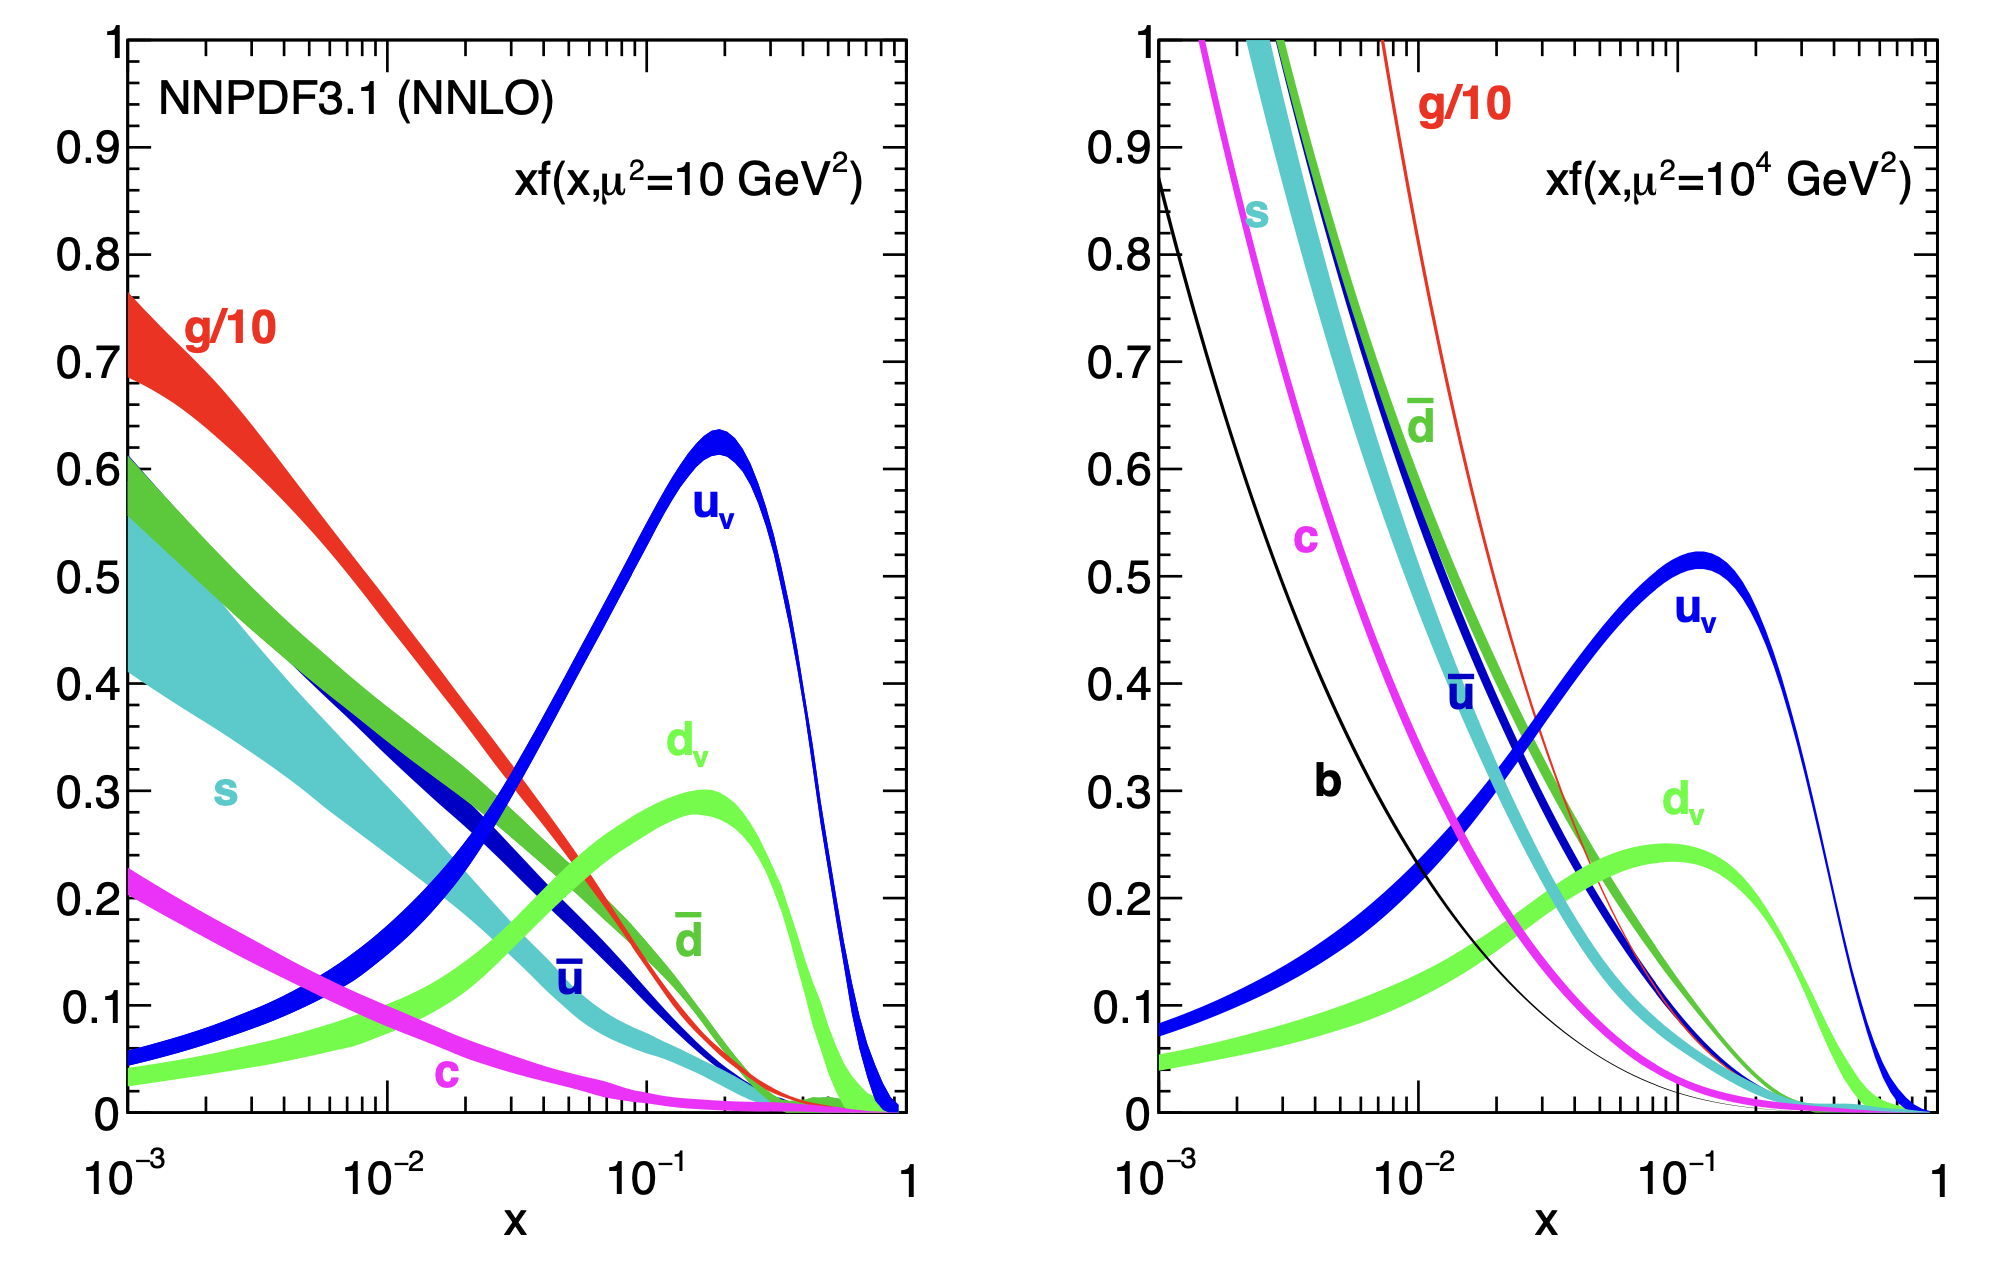
\includegraphics[width=0.95\textwidth]{protonPDFs}
\caption{Gluon and quark PDFs for the proton obtained in NNLO NNPDF3.1 analysis \cite{Ball_2017} at scale $\mu_F^2=10\,GeV^2$ (left) and $\mu_F^2=10^4\,GeV^2$ (right).}
\end{center}
\end{figure}

Gluon and sea quark distributions grow at small $x$, in particular gluon dominates at small longitudinal momentum fraction. Differently to what typically observed in elementary scattering processes, cross sections in hadron colliders increase with the energy. Indeed, we need smaller $x$ in order to produce the same mass state and the cross section grows due to the behavior of PDFs at small $x$.\\
For example, the Higgs production ($m_H\simeq 125\,GeV$) in a collision at $14\,TeV$ is dominated by gluons because, from kinematical considerations, the needed momentum fraction is $x\simeq 10^{-2}$. For this reason, the interaction between two gluons through a quark loop in order to produce the Higgs boson is the main channel for the production of this scalar particle. This process is known as the \textit{gluon gluon fusion} (ggF).\\

After the hard collision, the QCD products undergo a \textit{jet fragmentation process} due to the confinement property of strong interactions. Indeed, the signals in the detector are hadrons with high transverse momentum forming jets.\\
Firstly, soft radiations are emitted from final states of the hard scattering process. The probability of no gluon emissions above some transverse momentum is encoded in the Sudakov form factor which is used to generate the gluon distribution by Monte Carlo (MC) methods. In order to complete a real description of an event simulation, we have to include the hadronisation. Only a color-neutral collection of partons can be observed as an isolate system, then the MC event generators should implement this process. Currently, the most used implementations are based on string \cite{Andersson:1983ia} or cluster \cite{Chahal:2022rid} hadronisation models.\\
\newpage

The parton level cross section $\hat \sigma$ describes the hard scattering and is related to the fundamental interactions between elementary fields. This prediction can be calculated perturbatively because of the asymptotic freedom of QCD. The cross section is related to the squared matrix element,
\begin{align*}
	\hat \sigma(f_1 f_2 \rightarrow X)=\frac{\mathcal{S}}{2 \hat s} \int \dd \Pi_n \, \delta^{(4)}\left(\text{total momentum}\right) \left| \mathcal{A}(f_1 f_2 \rightarrow X)\right|^2,
\end{align*}
where $\mathcal{S}$ is a symmetry factor related to the identical particles in the final state and $\hat s$ is the center of mass energy for the parton process. We have to integrate over the Lorentz invariant phase space measure for the $n$ outgoing particles which are in the set $X$ and have momenta $q_i$,
$$
	\int \dd \Pi_n = \prod_i \int \frac{\dd^3 q_i}{2E_i (2\pi)^3}.
$$
The scattering amplitude $\mathcal{A}(f_1 f_2 \rightarrow X)$ is the fundamental ingredient which describes the interaction between the elementary particles. It represents a bridge between the QFT model and the phenomenology. In order to compute the amplitude, according to the traditional approach we should start from the Lagrangian, extract the Feynman rules for propagators and interaction vertices, compute all the allowed Feynman diagrams and sum together. The number of diagrams quickly increases with the number of external asymptotic states and with the number of loops. Furthermore, in squaring the amplitude, we have to compute quantum interferences between Feynman diagrams and this increases the complexity of the calculation.\\
Firstly, we can fix the polarization of the asymptotic states, namely the helicity for massless particles. The complexity is reduced because different helicity configurations do not interfere in the squared amplitude. Then we have to compute only a sum of squared helicity amplitudes,
\begin{align*}
	\left| \mathcal{A}(a+\dots \rightarrow b+\dots)\right|^2= \sum_{h_a, h_b, \dots} | \mathcal{A}(a^{h_a} +\dots \rightarrow b^{h_b} +\dots)|^2.
\end{align*}
Surprising structures of helicity amplitudes were found indeed they are simpler than the expectation from a sum of many Feynman diagrams. The complexity of helicity amplitudes depends on how much they violate the helicity conservation. The simplest structures are observed in the subset of not-vanishing helicity amplitudes which describe the processes with the maximal helicity violation, known as MHV amplitudes. In 1986, Parke and Taylor \cite{Parke:1986gb} predicted the structure of MHV amplitudes in gauge theories for an arbitrary number of gluons in terms of rational functions of kinematic invariants.\\
Moreover, the unitarity of the theory shows a connection between the discontinuity of loop amplitudes and on-shell amplitudes with lower levels of precision.
Modern techniques have been developed in order to compute one-loop and two-loop amplitudes using generalisations of the unitarity approach. One of the main reasons of the complexity of traditional computations is related to gauge redundancy. Feynman diagrams are not individually invariants differently to the result, then strong cancellations arise only when we sum together all the contributions. On-shell methods use tree-level amplitude as the building blocks for predictions of higher precision level, then they fully exploit the gauge invariance of the theory.\\

The cross section for the Higgs boson ggF production is currently known at next-to-next-to-next leading order ($\text{N}^3\text{LO}$) in QCD corrections \cite{Anastasiou_2015}. NNLO is the current level of precision of QCD corrections for the Higgs production in association with a jet \cite{Boughezal_2015}. The complexity of the computation increases with additional jets indeed for the Higgs production with two jets only NLO QCD corrections was computed \cite{an_Deurzen_2013}. These predictions are calculated in the Higgs Effective Field Theory (HEFT) in which the dominant contribution to ggF, the top-quark loop, is integrated out in the limit of infinite top mass $m_t$. This method reduces the number of loops we have to compute by one, but it is necessary a good control of the validity of this approximation. NLO predictions with the full top-mass effects are computed for the Higgs+jet production \cite{Harlander_2012, Jones_2018}. HEFT seems to works because the Higgs mass is below $2m_t$, which is the case of phenomenological interest. However, the quality of the heavy-top limit is limited by effects on Higgs' transverse momentum $p_{t,H}$: HEFT is a good approximation for $p_{t,H}<200 GeV$ as one can see in the Figure [\ref{fig:pt}]. 
\begin{figure}[H]
\begin{center}
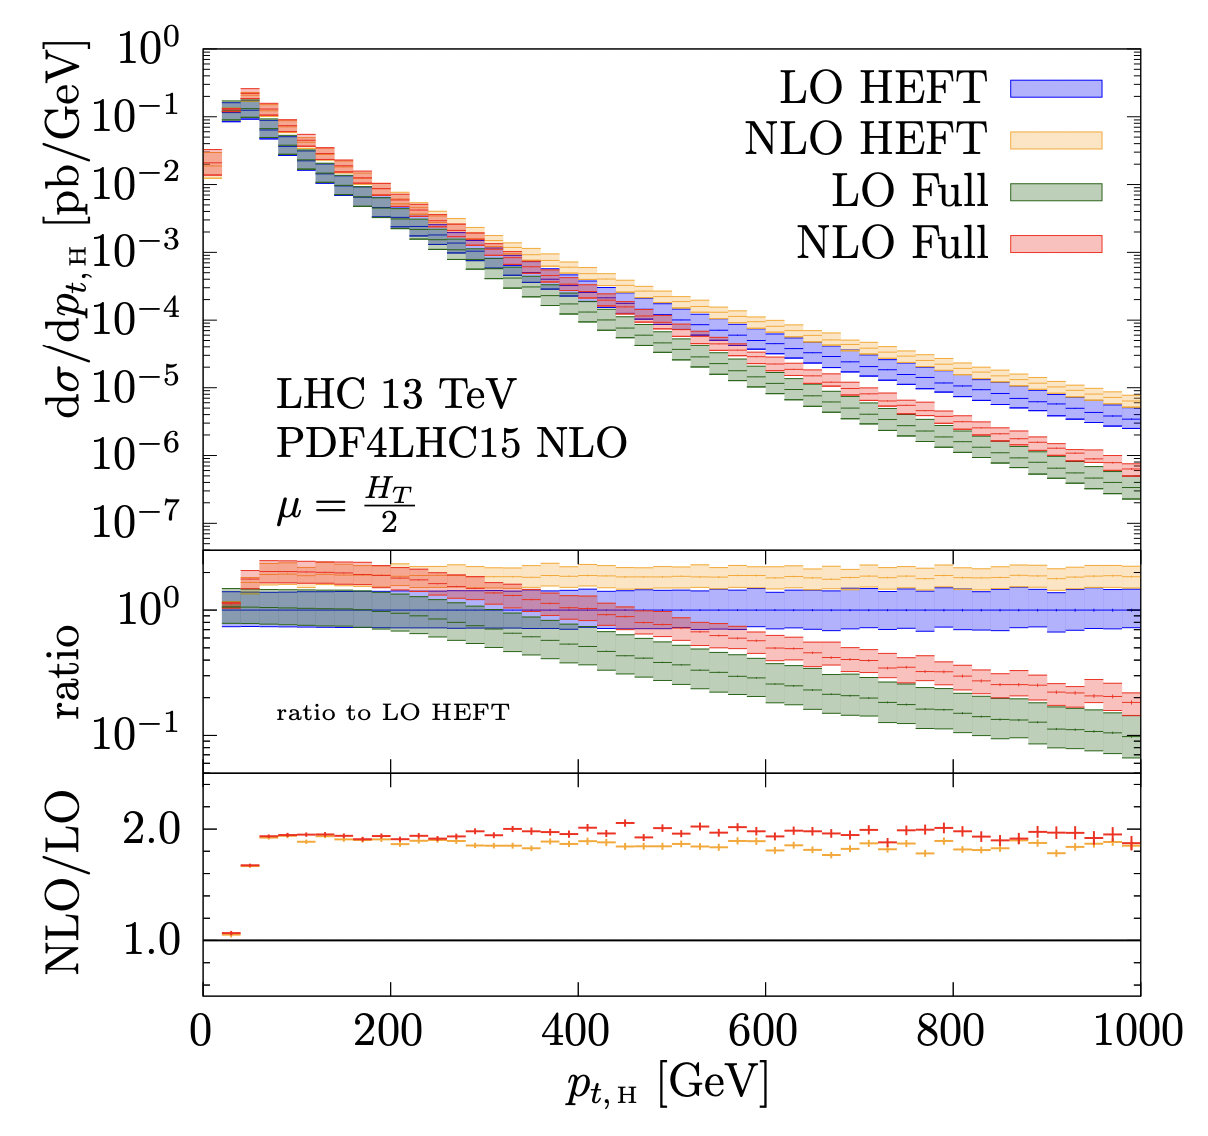
\includegraphics[width=0.6\textwidth]{Higgspt}
\caption{Higgs boson transverse momentum spectrum in QCD LO and QCD NLO for the Higgs+jet production. Comparison between the HEFT predictions and the results with the full top-mass dependence. For $p_t<200 GeV$ we observe a good agreement between the two approaches. \cite{Jones_2018}}
\label{fig:pt}
\end{center}
\end{figure}

In order to improve the level of precision for Higgs plus two jets, QCD two-loop virtual corrections represent a fundamental ingredient in NNLO computations. The desired two-loop amplitude $\mathcal{A}(gg\rightarrow Hgg)$ is not currently known in the HEFT. In an interesting version of the effective field theory, we can decompose the Higgs into two scalar fields $\phi$ and $\phi^\dagger$ whose interactions with gluons are endowed with self-dual properties. On-shell $\phi$ plus gluon amplitudes show simpler structures, in particular the MHV tree amplitude has the same form of Parke-Taylor formula.\\

In Chapter [\ref{onshellamp}], we review the spinor helicity formalism and some on-shell methods at tree and loop level. Led by the analogy between $\phi$+gluon and pure QCD MHV amplitudes, Chapter [\ref{secYM}] is devoted to the study of known one-loop and two-loop amplitudes in the all-plus sector of Yang-Mills. This represents an interesting background to learn the generalised unitarity methods in four dimensions and cuts in generic dimensions.\\
In the next chapter, we introduce the self-dual Higgs theory and we will review some useful tree and one-loop amplitudes which describe the coupling between the self-dual Higgs ($\phi$) and gluons. Also for the study of these amplitudes we implement some on-shell techniques discussed in Chapter [\ref{onshellamp}].\\
In Chapter [\ref{ch:cuts}], we compute the discontinuities of the two-loop amplitude which involves the self-dual Higgs field ($\phi$) and four gluons with positive helicity. The cut-constructible part of this amplitude represents the original result of this project.\\
In the first appendix we report the notations and the expressions for the one-loop scalar integrals.\\
In App. [\ref{appC}], we describe the computation of quadruple cuts, a generalised unitarity method applied to investigate the box contributions in the amplitude.\\
App. [\ref{phi+3g}] is devoted to the computation of the discontinuities for the amplitude at lower multiplicity considering the self-dual Higgs and only three gluons. These could be useful as a preliminary introduction for the cut computations before studying the more challenging case in Chapter [\ref{ch:cuts}]. The computation is necessary in order to check the collinear limit of the $\phi$ plus four gluon amplitude.


\chapter{On-shell techniques}	\label{onshellamp}

\section{Color decompositions in QCD}
\subsection{QCD Lagrangian and Feynman rules}
Quantum chromodynamics (QCD) is a gauge theory based on the non-abelian group $SU(N_c)$. This model describes the strong interaction between gluons and fermions. The gauge group of QCD is $SU(3)$, but we can consider a generic number of possible colors $N_c$. In addition to the utility in having an explicit dependence on $N_c$, the limit in which $N_c$ goes to infinity is sometimes useful.\\
The dynamics is described by the Lagrangian density:
$$
	\mathcal{L}_{QCD}=-\frac{1}{4} G^{a}_{\mu\nu} G^{a\mu\nu}+\sum_{f=1}^{n_f} \bar \psi_f^{i} \left(i\gamma^\mu D_\mu^{i j}-m_f \delta^{i j}\right)\psi_f^j.
$$
The first contribution is described by the gluon field tensor which can be written in terms of the gluon field $A_\mu^a$:
$$
	G_{\mu\nu}^a=\partial_\mu A_\nu^a-\partial_\nu A_\mu^a+g_s f^{abc} A_{\mu}^b A_\nu^c.
$$
The index $f$ deals with the possible flavours of quarks described by the field $\psi_f^i$ which transforms into the fundamental representation of $SU(N_c)$. Thus, in the Dirac term we used the covariant derivative in the fundamental representation:
$$
	(D_\mu)_{ij}=\delta_{ij}\partial_\mu-\frac{ig_s}{\sqrt2} T^a_{ij} A^a_{ij}.
$$
The generators $T^a_{ij}$ are Hermitian traceless $N\cross N$ matrices which carry quark indeces $i,j=1,\dots,N_c$ and a gluon index $a=1,\dots, N_c^2-1$. They obey the commutation relation
$$
	[T^a,T^b]=i\sqrt{2}f^{abc}T^c
$$
with the gauge group structure constants $f^{abc}$. The normalisation is chosen in order to avoid a proliferation of factors $\sqrt{2}$ in the sub-amplitudes. We select a diagonal basis for the generators such that
$$
	\text{tr}\left(T^a T^b\right)=\delta^{ab}.
$$
In the QCD case, explicit expressions for the $SU(N_c)$ generators can be written in terms of Gell-Mann matrices.\\
In order to extract the Feynman rules, we need to insert a gauge fixing term
$$
	\mathcal{L}_{GF}=-\frac{1}{2\xi} (\partial^\mu A_\mu^a)^2
$$
Studying the kinetic term of the Lagrangian, we can deduce the propagators for gluons and quarks.
\begin{align*}
	&\feynmandiagram [inline=(b.base), horizontal= a to b]
	{
		a [particle=\(a\mu\)] -- [gluon, momentum=\(k\)] b  [particle=\(b\nu\)],
	}; = \frac{\delta^{ab}}{k^2+i0^+}\left(\eta_{\mu\nu}+(\xi-1)\frac{k_\mu k_\nu}{k^2}\right)\\
	&\feynmandiagram [inline=(b.base), horizontal= a to b]
	{
		a [particle=\(i\)] -- [fermion, momentum=\(k\)] b  [particle=\(j\)],
	}; = \delta_{ij}\frac{\slashed k-m}{k^2-m^2+i0^+}
\end{align*}
We will specialise to the Feynman guage $\xi=1$ in which we have a simplification of the gluon propagator. 
On the other hand, the vertices are defined from the interaction terms.
\begin{align*}
	\feynmandiagram [inline=(b.base), horizontal= a to c]
	{
		a [particle=\(a\mu\)]-- [gluon, rmomentum'=\(p\)] b -- [gluon, momentum=\(q\)] c [particle=\(b\nu\)];
		b -- [gluon, momentum=\(r\)] d [particle=\(c\rho\)];
	}; = &g_s f^{abc} \left[(q-r)_\mu \eta_{\nu\rho}+(r-p)_\nu \eta_{\rho\mu}+(p-q)_\rho \eta_{\mu\nu}\right]\\[-20pt]
	\feynmandiagram [scale=0.8, inline=(b.base),horizontal= a to c, vertical= a to d]
	{
		a [particle=\(a\mu\)]-- [gluon] b -- [gluon] c [particle=\(c\rho\)],
		d [particle=\(d\sigma\)]-- [gluon] b -- [gluon] e [particle=\(b\nu\)],
	}; 
	=
	&\begin{aligned}
	&\\
	&\\[8pt]
	&-ig_s^2 \left[f^{abe}f^{cde}(\eta_{\mu\rho}\eta_{\nu\sigma}-\eta_{\mu\sigma}\eta_{\nu\rho})\right.\\
	&\left. +f^{ace}f^{dbe}(\eta_{\mu\sigma}\eta_{\rho\nu}-\eta_{\mu\nu}\eta_{\rho\sigma})\right.\\
	&\left. +f^{ade}f^{bce}(\eta_{\mu\nu}\eta_{\sigma\rho}-\eta_{\mu\rho}\eta_{\sigma\nu})\right]\\
	\end{aligned}\\
	\feynmandiagram [scale=0.87,baseline=(d.base), horizontal=d to b] {
a [particle=\(i\)]-- [fermion] b -- [fermion] c [particle=\(j\)],
b -- [gluon] d [particle=\(a\mu\)], };
= & \frac{i g_{s}}{\sqrt2} \gamma^{\mu} (T^a)_{ij}
\end{align*}
From the Fadeev-Popov approach, we know that the Lagrangian is not complete if we do not add ghosts. However, their contributions play no rule at tree-level and we will construct loop amplitudes using unitarity methods considering only physical external states which do not include ghost. 

\subsection{Counting diagrams}
In order to understand the complexity of perturbative computations when the number of legs increases, we can consider the pure gluon sector of QCD. For any diagram in the Yang-Mills theory we assign a monomial $G=g^\alpha v^\beta$, where $\alpha$ corresponds to the number of inner and external legs, while $\beta$ is the number of three-point vertices. Starting from a diagram with $n$ gluons, we can construct the contributions for the amplitude with $(n+1)$ gluon acting with differential operators on the monomials. \cite{Caravaglios_1999}
\begin{align*}
	\feynmandiagram [inline=(b.base), horizontal= a to b]
	{
		a -- [gluon] b;
	}; \mapsto
	\feynmandiagram [inline=(b.base), horizontal= a to c]
	{
		a -- [gluon] b -- [gluon] c;
		b -- [gluon] d;
	};
	\hspace{0.5cm} \boxed{\leftrightarrow} \hspace{0.5cm}
	& g \xmapsto{g^3 v \partial_g} g^3v\\
	\feynmandiagram [inline=(b.base), horizontal= a to c]
	{
		a -- [gluon,] b -- [gluon] c;
		b -- [gluon] d;
	}; \mapsto
	\feynmandiagram [scale=0.8, inline=(b.base),horizontal= a to c, vertical= a to d]
	{
		a -- [gluon] b -- [gluon] c,
		d -- [gluon] b -- [gluon] e,
	};
	\hspace{0.5cm} \boxed{\leftrightarrow} \hspace{0.5cm}
	& gv^3 \xmapsto{g \partial_v} g^4
\end{align*}
Thus we construct the monomial associated to $(n+1)$ gluons through the following differential operator:
$$
	G_{n+1}=\left(g^3 v \frac{\partial}{\partial g}+g\frac{\partial}{\partial v}\right) G_n.
$$
The number of diagrams for a tree-level amplitude with $n$ external gluons is obtained setting $g$ and $v$:
$
	N(G_n)=G_n(g=1,v=1).
$
Using this simple trick, we can count the number of diagrams for tree-level amplitudes involving only gluons in order to observe the rapid growth of complexity \cite{Badger:2016uuq}.
\begin{table}[h!]
\centering
 \begin{tabular}{||c c c c c c c c||} 
 \hline
 $N(G_3)$ & $N(G_4)$ & $N(G_5)$ & $N(G_6)$ & $N(G_7)$ & $\dots$ & $N(G_{10})$ &\\ [0.5ex] 
 \hline\hline
 $1$ & $4$ & $25$ & $220$ & $2485$ & \dots & $> 10^7$ &\\ 
 \hline
 \end{tabular}
\end{table}
\\This counting shows the necessity of reorganize the amplitudes in order to reduce the rapid combinatorial growth due to the $SU(N_c)$ color structure.

\subsection{Color factors and partial amplitudes}
Feynman rules show a structure in which we can recognise a color contribution described by the structure constants $f^{abc}$ or the matrices $T^a$ and a kinematical term. The basic idea \cite{Dixon:1996wi} consists in splitting the computation of QCD amplitudes into two parts: colour and kinematics contributions. Then we have to use a basis for colour factors: a possible choice is the reorganisation of QCD dofs in order to eliminate $f^{abc}$ in the Feynman rules in favor of the generators $T^a$.\\
With our conventions, the structure constants can be given by
\begin{align}
	f^{abc}=-\frac{i}{\sqrt{2}}\text{tr}\left([T^a,T^b]T^c \right).	\label{ftoT}
\end{align}
Pictorially, this relation can be described keeping in mind the color structure of Feynman rules.
\begin{equation*}
	 \feynmandiagram [inline=(v.base), vertical=i1 to v] 
	 { i1 -- [gluon] v -- [gluon] i2, v -- [gluon] i3,
	 };
	 =
	 \feynmandiagram [scale=0.7, baseline=-1.5cm, vertical=i1 to v1] 
	 { i1 -- [gluon] v1,
	 v2 -- [gluon] i2, 
	 v3 -- [gluon] i3,
	 v1 -- [fermion, out=180, in=120] v2 -- [fermion, out=-60, in=-120] v3 -- [fermion, out=60, in=0] v1, 
	 };
	 -
	 \feynmandiagram [scale=0.7, baseline=-1.5cm, vertical=i1 to v1] 
	 { i1 -- [gluon] v1,
	 v2 -- [gluon] i2, 
	 v3 -- [gluon] i3,
	 v1 -- [anti fermion, out=180, in=120] v2 -- [anti fermion, out=-60, in=-120] v3 -- [anti fermion, out=60, in=0] v1, 
	 };
\end{equation*}
Another important relation is the Fierz identity for $SU(N_c)$ matrices,
\begin{align}
	(T^a)_{i_1}^{j_1}(T^a)_{i_2}^{j_2}=\delta_{i_1}^{j_2}\delta_{i_2}^{j_1}-\frac{1}{N_c}\delta_{i_1}^{j_1}\delta_{i_2}^{j_2}	\label{FierzSU}
\end{align}
which corresponds to the completeness relation for the generators \cite{Henn:2014yza}. In addition, the last contribution guarantees the traceless condition.\\ %This identity is illustrated graphically with the following 't Hooft representation
%\begin{equation*}
%	 \feynmandiagram [inline=(a.base), horizontal=a to b] 
%	 { i1 -- [fermion] a -- [fermion] i2, a -- [gluon] b, 
%	 f1 -- [fermion] b -- [fermion] f2,
%	 };
%	 =
%\end{equation*}
It is sometimes convenient to consider also the $U(N_c)=SU(N_c)\cross U(1)$ gauge group. The additional generator is proportional to the identity,
$$
	(T^{a_{U(1)}})_i^j=\frac{1}{\sqrt N_c} \delta_i^j.
$$
The normalisation is chosen so that the $U(N_c)$ Fierz identity becomes
\begin{align}
	(T^c)_{i_1}^{j_2} (T^c)_{i_3}^{j_4}=\delta_{i_1}^{j_4}\delta_{i_3}^{j_2}.	\label{FierzU}
\end{align}
The $U(1)$ generator can be associated to a photon. It is colorless and presents a vanishing structure constants $f^{a_{U(1)}bc}=0$ for all $b,c$. Therefore, we do not observe any coupling between photons and gluons, while quarks carry charge under this abelian generator. In tree-level amplitudes with only gluons or at most a $q\bar q$ pair in the set of asymptotic states, the photon does not play any rule and, for this reason, we can directly simplify the computation using the identity (\ref{FierzU}) instead of (\ref{FierzSU}).\\
\subsubsection{Structure of tree gluon amplitudes}
We want to replace systematically in every Feynman diagram all the factors $f^{abc}$ in terms of the generators $T^a$. For example, we can compute the color structure of the four-gluon tree amplitude in the three channels:
$$
	c_s=f^{abe}f^{ecd}, \hspace{1cm}c_t=f^{ace}f^{edb}, \hspace{1cm}c_u=f^{ade}f^{ebc},
$$
where $a,b$ are the color indices of inner gluons and $c,d$ are associated to the out states.\\
Using equations (\ref{ftoT}, \ref{FierzU}), we can simplify the product of two structure constants,
\begin{align*}
	f^{abe}f^{ecd}&=-\frac{1}{2}\text{tr}\left( [T^a,T^b]T^e\right)\text{tr}\left([T^c,T^d]T^e\right)=-\frac{1}{2}\text{tr}\left([T^a,T^b][T^c,T^d]\right).
\end{align*}
Then we can write the four gluon amplitude as \cite{2014}
$$
	\mathcal{A}^{tree}(1,2,3,4)=g^2\left[A^{tree}(1,2,3,4)\text{tr}(T^{a_1}T^{a_2}T^{a_3}T^{a_4})+\text{perms of }(234)\right]
$$
where $A^{tree}(1,2,3,4)$ is known as a color-ordered partial amplitude.\\
We can generalise for an arbitrary number of gluons, then the colour decomposition for a gluon amplitude at tree-level is \cite{Mangano:1988kk}
\begin{align}
	\mathcal{A}^{tree}(1,2,\dots,n)=g^{n-2} \sum_{\sigma\in S_n/\mathbb{Z}_{n}} \text{tr}\left(T^{a_{\sigma_1}}\dots T^{a_{\sigma_n}}\right) A^{tree}(\sigma(1),\sigma(2),\dots,\sigma(n))	\label{trbdectree}
\end{align}
where the sum is over all the possible non-cyclic permutations of gluons.\\
Partial amplitudes show interesting relations:
\begin{enumerate}
	\item they are cyclically invariant, then we can fix the position of a gluon in the colour decomposition
	$$
		\mathcal{A}^{tree}(1,2,\dots,n)=g^{n-2} \sum_{\sigma\in S_{n-1}} \text{tr}\left(T^{a_{\sigma(1)}}\dots T^{a_{\sigma(n)}}\right) A^{tree}(1,\sigma(2),\dots,\sigma(n));
	$$
	\item they satisfy a reflection identity
	$
		A^{tree}(n,n-1,\dots,2,1)=(-)^n A^{tree}(1,2,\dots,n);
	$
	\item if we insert the $U(1)$ generator the amplitude must vanish and this yields to a linear combination known as photon decoupling identity,
	$$
		\sum_{\sigma\in \mathbb{Z}_{n-1}} A^{tree}(1,\sigma(2),\dots,\sigma(n))=0.
	$$
\end{enumerate}
The last two relations are included in a more general equation found by Kleiss and Kuijf \cite{Kleiss:1988ne}.\\
Partial amplitudes reduce the complexity, indeed we can observe a polynomial growth of necessary independent graphs for the computation of amplitudes with a different number $n$ of legs \cite{Badger:2016uuq}.
\begin{table}[H]
\centering
 \begin{tabular}{|| c | c c c c c||} 
 \hline
 $n$ & $3$ & $4$ & $5$ & $6$ & $7$ \\ [0.5ex] 
 \hline\hline
 $\mathcal{A}_n$ & $1$ &$4$ &$25$ & $220$ & $2485$ \\ 
 \hline\hline
  $A_n$ & $1$ &$3$ &$10$ & $38$ & $154$ \\ 
 \hline
 \end{tabular}
 \caption{\label{tab:FCounting}Number of needed graphs for the amplitude $\mathcal{A}_n$ and the partial one $A_n$ in function of the number $n$ of external gluons.}
\end{table}
\subsubsection{Tree amplitudes with gluons and a quark-antiquark pair}
Let us consider the scattering $q\bar{q}\rightarrow gg$. At tree-level, the amplitude is the sum of three diagrams.
\begin{align*}
\feynmandiagram [small,horizontal=a to b, inline=(a.base)] {
i1 [] -- [fermion] a -- [fermion] i2 [],
a -- [gluon] b,
f1 [] -- [gluon] b -- [gluon] f2 [],
};
\hspace{0.3cm}+\hspace{0.3cm}
\begin{aligned}
\feynmandiagram[small, vertical'=a to b]{
        i1 -- [gluon] a []
            -- [fermion] f1 [],
        a -- [anti fermion] b [],
        i2 -- [gluon ] b
            -- [anti fermion] f2
    }; 
    \end{aligned}
    \hspace{0.3cm}+\hspace{0.3cm}
     \begin{aligned}
     \begin{tikzpicture}
     \begin{feynman}
      \diagram [small, vertical=a to b] {
      i1 []
      -- [anti fermion] a
      -- [draw=none] f1 [],
      a -- [anti fermion] b,
      i2 []
      -- [fermion] b
      -- [draw=none] f2 [],
      };
      \diagram* {
          (b) -- [gluon] (f1),
          (a) -- [gluon] (f2),
      };
      \end{feynman}
      \end{tikzpicture}
      \end{aligned}
\end{align*}
For the first diagram, the colour factor can be reduced using the relation (\ref{ftoT}),
$$
	i\sqrt{2}f^{a_3a_4b}T^b=T^{a_3}T^{a_4}-T^{a_4}T^{a_3}.
$$
Thus the amplitude can be written in the following form,
$$
	\mathcal{A}^{tree}(1_{\bar q},2_q,3_g,4_g)=g^2\left(A^{tree}(1_{\bar q},2_q,3_g,4_g)T^{a_3}T^{a_4}+A(1_{\bar q},2_q,4_g,3_g)T^{a_4}T^{a_3}\right).
$$
One can demonstrate the following decomposition which generalises the expansion of the amplitude for a quark pair and an arbitrary set of gluons \cite{Mangano_1991},
$$
	\mathcal{A}^{tree}(1_{\bar q},2_q,3_g,\dots,n_g)=g^{n-2}\sum_{\sigma\in S_{n-2}}\left(T^{a_{\sigma_3}}\dots T^{a_{\sigma_n}}\right)_{i_1}^{j_2}A^{tree}(1_{\bar q},2_q,\sigma(3)_g,\dots,\sigma(n)_g).
$$
In conclusion, we can apply this reorganisation also at the loop level \cite{Bern:1990ux}. In contrast to what observed at tree level, loop amplitudes show a colour structure that does not only contain single traces. We will specify the colour decompositions in Chapter [\ref{secYM}].
\section{Spinor-helicity formalism}
In this section we will show that the kinematics of massless particle scattering in the Minkovski space $SO(1,3)$ can be described by two copies of $SU(2)$ Weyl spinors. The formalism we will review provides more compact expressions for scattering amplitudes.
\subsection{Massless particles} 
For massless particles, the projection of the spin onto the axis of the three-momentum is a conserved quantity known as helicity
$$
	h=\frac{\mathbf{p}\cdot \mathbf{S}}{|\mathbf{p}|}.
$$
We introduce the spinor-helicity language to describe efficiently on-shell scattering amplitudes. As a starting point, using Weyl basis, we can write
$$
	\slashed p =\gamma^\mu p_\mu=\begin{pmatrix}
		0 & p_{\alpha \dot\alpha } \\
		p^{\dot \alpha \alpha} & 0
	\end{pmatrix}
$$
where we introduced two objects with spinor indices. Explicitly we have
$$
	p^{\dot\alpha \alpha}=\bar \sigma^{\dot\alpha \alpha}_\mu p^\mu=
	\begin{pmatrix}
		p^{+} & \bar p_\perp \\
		p_\perp & p^{-}
	\end{pmatrix}, \hspace{0.7cm} p_{\alpha \dot\alpha}=\sigma_{\alpha \dot\alpha}^\mu p_\mu=
	\begin{pmatrix}
		-p^{-} & p_\perp \\
		\bar p_\perp & -p^{+}
	\end{pmatrix}
$$
where $\bar \sigma^{\dot\alpha \alpha}_\mu=(\mathbb{1},\sigma)$ and we introduce the light-cone coordinates $p^{\pm}=p^0\pm p^3$, $p_\perp=p^1+ip^2$.\\
In Weyl basis, Dirac equations $\slashed p u(p)=\slashed p v(p)=0$ can be converted into
\begin{align}
	p^{\dot \alpha \alpha} \lambda_{\alpha}=0, \hspace{0.5cm} p_{\alpha \dot\alpha} \tilde \lambda^{\dot \alpha}=0
	\label{Direq}
\end{align}
where $(\lambda, \tilde\lambda)$ is a pair of Weyl spinors respectively in the $(1/2,0)$ and $(0,1/2)$ representations of Lorentz group. They represent the building blocks for the solutions with defined helicity,
$$
	|p\rangle :=u_+(p)=v_-(p)=\begin{pmatrix}
		\lambda_\alpha\\
		0
	\end{pmatrix}, \hspace{0.5cm}
	|p] := u_-(p)=v_+(p)=\begin{pmatrix}
		0 \\
		\tilde \lambda^{\dot\alpha}
	\end{pmatrix}.
$$
Spinor indices can be raised and lowered with the Levi-Civita symbol $\epsilon$,
$$
	\lambda^\alpha:= \epsilon^{\alpha\beta} \lambda_\beta, \hspace{0.5cm} \tilde \lambda_{\dot\alpha}:= \epsilon_{\dot\alpha\dot\beta} \tilde\lambda^{\dot \beta},
$$
and using these objects it will be useful to define
$$
	\langle p| :=\begin{pmatrix}
		\lambda^\alpha & 0
	\end{pmatrix}, \hspace{0.5cm}
	[ p| :=\begin{pmatrix}
		\tilde\lambda_{\dot\alpha} & 0
	\end{pmatrix}.
$$
Using the properties of Pauli matrices, it is easy to show that
$$
	p_i^{\dot \alpha \alpha} p_j^{\dot \beta \beta} \epsilon_{\alpha\beta} \epsilon_{\dot \alpha \dot \beta}=2 p_i\cdot p_j.
$$
Using these property we observe that
$$
	0=p_i^2=\frac{1}{2}p_i^{\dot \alpha \alpha} p_i^{\dot \beta \beta} \epsilon_{\alpha\beta} \epsilon_{\dot \alpha \dot \beta}=\det\left(p_i^{\dot \alpha\alpha}\right),
$$
therefore we can decompose $p^{\dot\alpha \alpha}$ using only a pair $(\lambda,\tilde \lambda)$ which parametrizes a $2\cross2$ matrix with rank one. We can fix the normalisation of Weyl spinors imposing
$$
	p_i^{\dot \alpha \alpha}=\tilde \lambda_i^{\dot\alpha}\lambda_i^\alpha.
$$
Solving the equations (\ref{Direq}) with the previous condition, we obtain the explicit expressions
$$
	\lambda^\alpha=\frac{1}{\sqrt{p^+}}\begin{pmatrix}
		p^+ \\
		p_\perp
	\end{pmatrix},
	\hspace{0.5cm}
	\lambda^\alpha=\frac{1}{\sqrt{p^+}}\begin{pmatrix}
		p^+ \\
		\bar p_\perp
	\end{pmatrix}.
$$
We summarise some important identities for $SU(2)$ spinors and for their inner products.
\begin{enumerate}
	\item Angle and square brackets define the basic spinor invariants which are \textbf{antisymmetric}.
	\begin{align*}
		\langle ij\rangle&:= \lambda_i^\alpha \lambda_{j\alpha}=\epsilon_{\alpha\beta} \lambda_i^\alpha \lambda_j^\beta=-\epsilon_{\beta\alpha}\lambda_j^\beta \lambda_i^\alpha =-\langle ji \rangle\\
		[ij]&:= \tilde\lambda_{i\dot\alpha}\tilde\lambda_j^{\dot\alpha}=\epsilon_{\dot\beta\dot\alpha}\tilde\lambda_{i}^{\dot\beta}\tilde \lambda_{j}^{\dot\alpha}=-[ji]
	\end{align*}
	\item The \textbf{projection operator} is
	$$
		| i \rangle[ i |= \frac{1+\gamma_5}{2}\slashed p_i, \hspace{0.5cm} |i]\langle i|=\frac{1-\gamma_5}{2}\slashed p_i,
	$$
	and we can write 
	$
		\slashed p=|i\rangle[i|+|i]\langle i|.
	$
	We will often use the following relations in order to write traces in terms of spinor products and viceversa,
	\begin{align*}
		\langle z abc\dots xy z]=\langle z a \rangle [a b] \langle b c\rangle \dots \langle x y \rangle [y z]&= \tr \left(|a\rangle [a||b]\langle b| \dots |y \rangle[y||z]\langle z|\right)\\
		&=\tr\left(\frac{1+\gamma_5}{2}\slashed a \slashed b \dots \slashed y \slashed z\right)=:\tr_+(ab\dots yz)\\
		[z abc\dots xy z\rangle=[z a]\langle ab \rangle [bc] \dots [xy]\langle y z\rangle&=\tr\left(\frac{1-\gamma_5}{2}\slashed a \slashed b \dots \slashed y \slashed z\right)=:\tr_-(ab\dots yz).
	\end{align*}
	\item \textbf{Mandelstam invariants} can be written in terms of spinor products,
	$$
		s_{ij}:=(p_i+p_j)^2=2p_i\cdot p_j=p_i^{\alpha\dot\alpha}p_{j\alpha\dot\alpha}=\langle ij \rangle[ij].
	$$
	Viceversa we have
	$$
		\langle ij \rangle= e^{i \theta_{ij}} \sqrt{|s_{ij}|}, \hspace{0.5cm} [ij]=-e^{-i\theta_{ij}}\sqrt{|s_{ij}|}
	$$
	where $\theta_{ij}$ is a phase that can be written in terms of the components of $p_i^\mu$ and $p_j^\mu$ \cite{Henn:2014yza}.\\
	The on-shell condition $s_i:=p_i^2=0$ is manifest from the antisymmetry.
	\item Although this formalism naturally imposes the on-shell property, there are still redundancies. The condition for the \textbf{momentum conservation} imposes a relation between the spinor products,
	$$
		\sum_i p_i^\mu=0 \iff \sum_i \langle a i \rangle [ib]=0
	$$
	for arbitrary spinors $\lambda_a, \tilde\lambda_b$.\\
	We will study a formalism in which the momentum conservation will be automatically satisfied [\ref{momtw}]. 
	\item Another important relation known as \textbf{Schouten identity} comes from a basic observation of linear algebra. Any Weyl spinor can be decomposed into a basis of two others:
	\begin{align}
		\lambda_k^{\alpha}=c_i \lambda_i^\alpha+c_j \lambda_j^\alpha.	\label{Schdec}
	\end{align}
	The previous relation can be contracted with $\lambda_{i\alpha}$  or $\lambda_{j\alpha}$. Then we obtain two equations which can be solved for the variables $c_i,c_j$. Then from the relation (\ref{Schdec}) we immediately obtain the desired identity,
	\begin{align}
		|k\rangle\langle ij \rangle+|i\rangle \langle jk \rangle+|j\rangle \langle ki \rangle =0.	\label{schouten}
	\end{align}
	\item The \textbf{Gordon identity}
	\begin{align}
		\frac{1}{2}\langle i|\gamma^\mu|i]=p_i^\mu		\label{Gordon}
	\end{align}
	can be immediately shown using the property of Pauli matrices
	$$
		A=\frac{1}{2}\text{tr}\left(\sigma^\mu A\right)\bar{\sigma}_\mu,
	$$
	valid for an arbitrary complex $2\cross2$ matrix $A$.
	\item Considering an arbitrary four-vector $q^\mu$ the following contractions give the same result,
	$$
		[i|\slashed q |j \rangle=\tilde\lambda_{i\dot\alpha} q^{\dot\alpha \alpha} \lambda_{j\alpha}, \hspace{0.5cm} \langle j|\slashed q|i]=\lambda_{j}^\alpha q_{\alpha\dot\alpha} \tilde \lambda_{i}^{\dot\alpha}.
	$$
	This observation implies the \textbf{charge conjugation of currents},
	$$
		[i|\gamma^\mu|j\rangle=\langle j|\gamma^\mu|i].
	$$
	\item The \textbf{Fierz rearrangement} formula is
	\begin{align}
		\langle i |\gamma^\mu|j]\langle k|\gamma_\mu |m]=-2\langle ik \rangle[jm].
	\end{align}
	Indeed we can make explicit the sums with spinor indices and use properties of Pauli matrices,
	\begin{align*}
		\langle i |\gamma^\mu|j]\langle k|\gamma^\mu |m]&=\lambda_{i}^\alpha \sigma_{\alpha \dot \alpha}^{\mu}\tilde\lambda_{j}^{ \dot \alpha}\lambda_{k}^\beta \sigma^\nu_{\beta \dot \beta}\tilde\lambda_{m}^{ \dot \beta} \eta_{\mu\nu}=\lambda_{i}^\alpha \tilde\lambda_{j}^{ \dot \alpha}\lambda_{k}^\beta \tilde\lambda_{m}^{ \dot \beta} \sigma_{\alpha \dot \alpha}^{\mu}\eta_{\mu\nu} \sigma^\nu_{\beta \dot \beta}\\
		&=\lambda_{i}^\alpha \tilde\lambda_{j}^{ \dot \alpha}\lambda_{k}^\beta \tilde\lambda_{m}^{ \dot \beta} 2 \epsilon_{\dot\alpha\dot\beta} \epsilon_{\alpha\beta}=-2\left(\epsilon_{\alpha\beta}\lambda_{i}^\alpha\lambda_{k}^\beta\right)\left(\epsilon_{\dot\beta\dot\alpha} \tilde\lambda_{j}^{ \dot \alpha}\tilde\lambda_{m}^{ \dot \beta}\right)=-2\langle ik \rangle[jm].
	\end{align*}
\end{enumerate}
We can also describe the polarisation vectors $\epsilon_h^\mu$ for massless gauge boson with momentum $p^\mu$ and helicity $h=\pm1$ if we choose a physical gauge (the light-like axial gauge). These vectors will depend on an auxiliary light-like reference vector $n$ which arbitrariness reflects gauge invariance. The explicit solution follows from
$$
	\begin{cases}
		\epsilon_h\cdot p=0,\\
		\epsilon_h\cdot n=0,\\
		\epsilon_h\cdot \epsilon_h=0,\\
		\epsilon_h\cdot \epsilon_{-h}=-1.
	\end{cases}
$$
We can decompose the polarisation vector in an appropriate basis which contains the vectors $p^\mu, n^\mu$ and two additional directions that spans the orthogonal subspace,
$$
	\epsilon^\mu_h(p,n)=a_h p^\mu+b_h n^\mu+\frac{c_h}{2} \langle p \gamma^\mu n]+\frac{d_h}{2}\langle n\gamma^\mu p].
$$
Inserting the previous expansion in the system of equations, we obtain with the help of Fierz identities the following conditions:
$$
	\begin{cases}
		b_h=0,\\
		a_h=0,\\
		c_{h}d_{h}=0,\\
		\frac{1}{2}\langle pn\rangle[np]\left(c_{h}d_{-h}+c_{-h}d_{h}\right)=-1.
	\end{cases}
$$
An allowed solution is
\begin{align}
	\epsilon_+^{\mu}(p,n)=-\frac{\langle n\gamma^\mu p]}{\sqrt{2}\langle np \rangle},\hspace{0.5cm}\epsilon_-^{\mu}(p,n)=\frac{\langle p\gamma^\mu n]}{\sqrt2 [pn]}.	\label{solepsilon}
\end{align}
\iffalse
\subsection{Massive case}
We will focus on the use of spinor helicity formalism for massless particles, but we can generalize this language to treat the properties of massive particles. For massive particles helicity is not a Lorentz-invariant object, but it is only defined with respect to the direction $n^\mu$ which breaks Lorentz-invariance. A possible approach is to find directly the eigenvectors of the momentum matrix $p_{\alpha\dot\alpha}$ to obtain the solutions for the massive Dirac equation. Alternatively, we can decompose the time-like momentum $p_i$ into two light-like directions: a null reference $q_i$ and the vector $$(p_i^b)^\mu=p-\frac{n^2}{2p\cdot n} n^\mu.$$
If $m\not=0$ the determinant of the momentum matrix does not vanish, therefore it has the maximum rank. Then we have to use two pairs of Weyl spinors to describe completely $p_{\alpha\dot\alpha}$. Precisely, we can use the following decomposition:
\begin{align*}
	p_i^{\dot\alpha \alpha}&=\bar \sigma_{\mu}^{\dot\alpha\alpha}p^\mu=\bar \sigma_{\mu}^{\dot\alpha\alpha}\left((p^b_i)^\mu+\frac{m^2}{2 n\cdot p}n^\mu\right)\\
	&=(\bar\sigma\cdot p^b_i)^{\dot\alpha\alpha}+\frac{m^2}{2p\cdot n}(\bar\sigma\cdot n)^{\dot\alpha\alpha}\\
	&=\tilde \lambda_{p^b_i}^{\dot\alpha}\lambda_{p^b_i}^{\alpha}+\frac{m^2}{2p\cdot n}\tilde \lambda_{n}^{\dot\alpha}\lambda_{n}^{\alpha}=:\tilde\lambda_{iI}^{\dot\alpha} \lambda_i^{\alpha I}.
\end{align*}
We can use an additional index $I=1,2$ to write the sum over a spinor basis which is defined by a double copy of spinor pairs. Details about the spinor-helicity formalism for all masses and spins can be found in \cite{Arkani-Hamed:2017jhn}.
\fi
\section{Momentum twistors} \label{momtw}
The spinor-helicity solves the on-shell constraints but we still have some redundancies. First of all, spinors must satisfy the momentum conservation:
\begin{align}
	\sum_i \lambda_i^a \tilde \lambda_i^{\dot a}=0.	\label{momcons}
\end{align}
In addition, starting from $6$ points, we observe other constraints in four dimension, indeed only four vectors are independent. For example in the case of six particle, we need to satisfy the Gram determinant condition,
$$
	\text{Gram}(p_1,p_2,p_3, p_4, p_5)=0,
$$
which gives a complicated polynomial relation.\\
The constraints reduce the number of independent variables to $3n-10$ for an amplitude with $n$ particles. This is exactly the number of dofs for an amplitude invariant under Poincarr\'e transformations with on-shell legs. Then all the conditions we have to impose are on-shellness, momentum conservation and Gram determinants. We want to construct a system of variables in which all the constraints are trivially satisfied.\\

The momenta $p_i^\mu$ can be used to construct graphically a figure with a closed contour due to the momentum conservation. We can use the colour ordering to select a specific polygon. We can decide to describe the kinematics using coordinates from the dual-space:
\begin{align*}
	&y_i^{\dot aa}-y_{i+1}^{\dot a a}=p_i^{\dot a a},\\
	&y_i^{\dot aa}-y_j^{\dot aa}=p_i^{\dot aa}+p_{i+1}^{\dot aa}+\dots + p_{j-1}^{\dot aa}.
\end{align*}
While the momenta $p_i$ are the sides, the variables $y_i$ correspond to vertices of the polygon. Dual coordinates make the momentum conservation manifest,
$$
	p_1+p_2+\dots+p_n=(y_1-y_2)+(y_2-y_3)+\dots+(y_n-y_1)=0.
$$
Using these coordinates and Dirac equation for massless particles, we can observe the so-called incident relation:
\begin{align}
	\lambda_i^{\alpha}(y_i)_{\alpha\dot\alpha}=\lambda_i^{\alpha}(y_{i+1})_{\alpha\dot\alpha}=:(\mu_i)_{\dot\alpha}.
	\label{incidentrel}
\end{align}
This define a new variable $\mu_i$ that we can use to describe the kinematics of the scattering process. More precisely, we can consider the set $Z_{iA}=(\lambda_{i\alpha},\mu_i^{\dot\alpha})$ as an alternative parametrisation compared with the use of four-momenta or spinor-helicity components $(\lambda_i,\tilde\lambda_i)$. $Z_i$ are called momentum twistors and their geometrical structure is described for example in \cite{2014}.\\
Any line based on the dual-space and defined by the points $y_i$ and $y_{i+1}$ corresponds to a point $Z_i$ in the twistor space. Viceversa, $y_i$ can be determined knowing $Z_i$ and $Z_{i+1}$, then for any line in the twistor space we observe a point in the manifold parametrised by the dual coordinates. Indeed we can show that
$$
	(y_{i})_{\alpha\dot\alpha}=\frac{\lambda_{i\alpha}\mu_{i-1,\dot\alpha}-\lambda_{i-1,\alpha}\mu_{i,\dot\alpha}}{\langle i-1|i \rangle}.
$$
Momentum twistors solve automatically the three types of constraints: on-shell conditions, momentum conservation and Gram determinants.\\
%We can describe the spinor $\tilde \lambda_i$ in terms of momentum twistor variables. The starting point is
%\begin{align*}
%	&\langle i | i-1 \rangle \langle i+1 | p_i= \langle i| i-1 \rangle \langle i+1 |(y_{i+1}-y_i)\\
%	&\langle i | i-1 \rangle \langle i+1 | i \rangle [i|=\langle i| i-1 \rangle \langle i+1 |y_{i+1}-\langle i| i-1 \rangle \langle i+1 |y_i
%\end{align*}
%and we can apply Schouten identity in the last addend,
%\begin{align*}
%	&\langle i | i-1 \rangle \langle i+1 | i \rangle [i|=\langle i| i-1 \rangle \langle i+1 |y_{i+1}+\langle i+1|i\rangle\langle i-1|y_i+\langle i-1|i+1\rangle \langle i| y_i\\
%	&\langle i-1 | i \rangle \langle i | i+1 \rangle [i|=\langle i | i-1 \rangle[\mu_{i+1}|+\langle i+1|i\rangle[\mu_{i-1}|+\langle i-1|i+1\rangle[\mu_i|\\
%	&\tilde\lambda_i=\frac{\langle i+1|i\rangle\mu_{i-1}+\langle i-1|i+1\rangle\mu_i+\langle i | i-1 \rangle\mu_{i+1}}{\langle i-1 | i \rangle \langle i | i+1 \rangle}.	\numthis \label{tildelambda}
%\end{align*}
In order to obtain a map between the spinor-helicity formalism and momentum twistors, we can write $\tilde \lambda_i$ in terms of $Z$. Using the incident relation (\ref{incidentrel}) and Schouten identity (\ref{schouten}), we can prove the relation
$$
	\tilde\lambda_i=\frac{\langle i+1|i\rangle\mu_{i-1}+\langle i-1|i+1\rangle\mu_i+\langle i | i-1 \rangle\mu_{i+1}}{\langle i-1 | i \rangle \langle i | i+1 \rangle}.
$$
Using the previous relation, we can directly prove the constraint (\ref{momcons}).
%In a compact form, the spinors $\tilde\lambda_i$ can be extracted from the dual twinstor,
%$$
%	W_i^A=(\tilde \mu_{i\alpha},\tilde \lambda^{\dot\alpha}_i)=\frac{\epsilon^{ABCD}Z_{i-1,B}Z_{i,C}Z_{i+1,D}}{\langle i-1|i\rangle\langle i|i+1\rangle}
%$$
Amplitudes can be parametrized using the holomorphic spinor products and momentum twistor 4-brackets:
\begin{align*}
	\langle ijkm \rangle= \epsilon^{ABCD}Z_{iA}Z_{jB}Z_{kC}Z_{mD}.
\end{align*}
In conclusion, a $n$-point massless amplitude can be described by $n$ momentum twistors. Any $4\cross n$ matrix for $Z$ will generate $n$ momenta such that all the constraints in four dimension are trivial. This matrix is parametrised by $(3n-10)$ variables $x_i$, but the choice is not unique. We used the following invertible parametrisation for the matrix.
\begin{align}
	Z=\begin{pmatrix}
		1 & 0 & \frac{1}{x_1} & \frac{1}{x_1}+\frac{1}{x_1x_2} & \frac{1}{x_1}+\frac{1}{x_1x_2}+\frac{1}{x_1x_2x_3}&  \dots&\frac{1}{x_1}+\dots+\frac{1}{x_1x_2\dots x_{n-3}} &\frac{1}{x_1}+\dots+\frac{1}{x_1x_2\dots x_{n-2}} \\
		0 & 1 & 1 & 1 & 1 &\dots& 1 &1\\
		0 & 0 & \frac{x_{n-1}}{x_{2}} & x_{n} & x_{n+1}& \dots  & x_{2n-6} & 1\\
		0 & 0 & 1 & 1 & x_{2n-5} & \dots  & x_{3n-11} & 1-\frac{x_{3n-10}}{x_{n-1}}
	\end{pmatrix}
	\label{momparamet}
\end{align}
A practical advantage of this choice is that the Gram determinant of four momenta becomes a perfect square in the momentum twistor variables. For example, if we consider a five-point amplitude, using (\ref{momparamet}) we have
\begin{align*}
	\text{Gram}(p_1,p_2,p_3, p_4)&=\left[\frac{x_1\left(x_2(1+2 x_3)x_4-(1+x_3)x_4(x_4-x_5)+x_2^2x_3(-1+x_5)\right)}{x_2}\right]^2\\
	&\equiv\left[\text{tr}(\gamma_5 \slashed p_1 \slashed p_2 \slashed p_3 \slashed p_4)\right]^2=: (\text{tr}_5)^2.
\end{align*}
The momentum twistor variables $\{x_1,\dots,x_5\}$ are equivalent to the set $\{s_{12},s_{23},s_{34},s_{45},s_{51},\tr_5\}$. Using the choice (\ref{momparamet}) we have rational maps which connect the two system of variables which describe the kinematical dependence of the amplitude for five massless particles.
\subsection{One off-shell leg}
The principal aim of this project is to study an amplitude involving four massless particles and a massive field. For this reason, we want to extend the formalism of momentum twistors for an amplitude with one off-shell external leg.\\
We can consider the massive leg with momentum $p_5$ as an off-shell particle which decays into two massless states.
\begin{center}
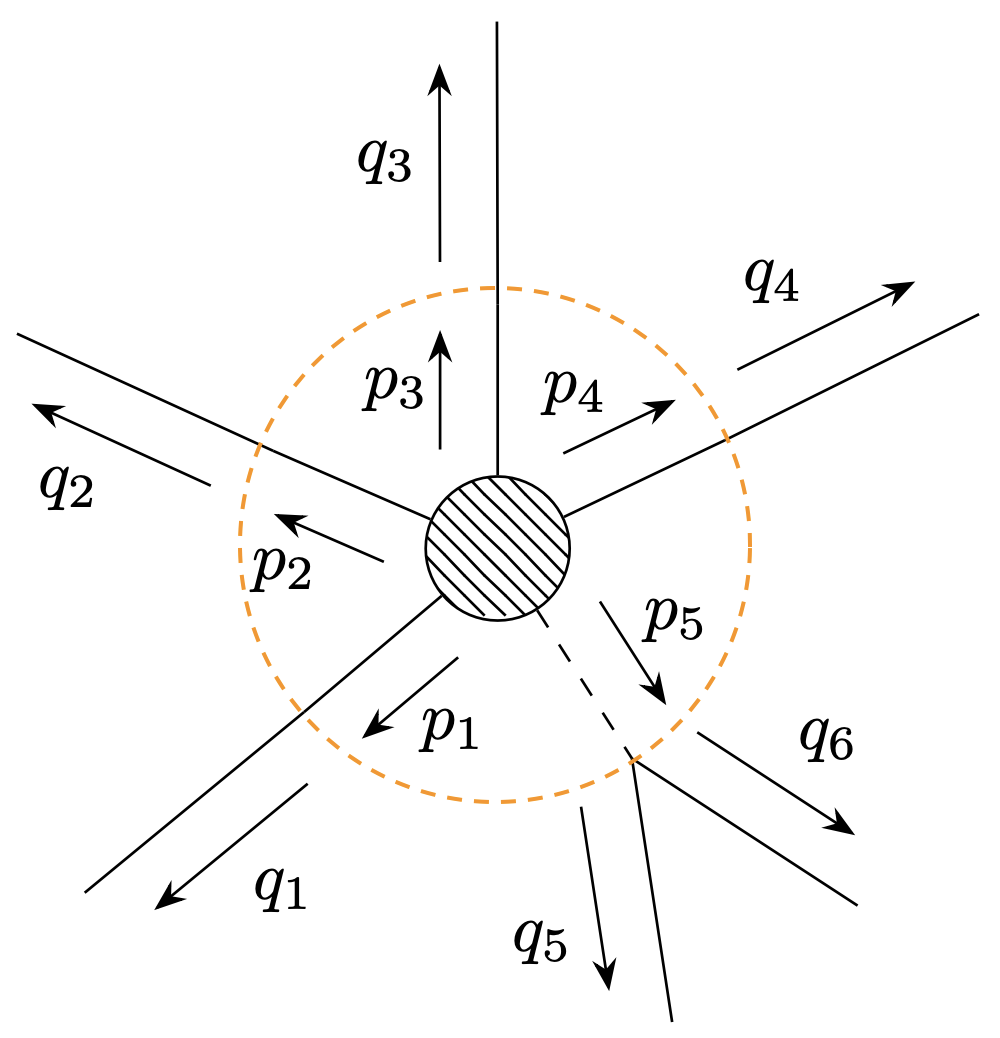
\includegraphics[width=0.40\textwidth]{massiveZ}
\end{center}
We can generate $q^\mu$ using momentum twistors for a $6$-point massless amplitude. The idea is to reconstruct $p_5^\mu$ in terms of twistor variables using the condition $p_5=q_5+q_6$.\\
Before doing it,  we need to carefully organise the degrees of freedom. Indeed an amplitude with six asymptotic massless states requires $3\cdot 6-10=8$ independent variables. On the other hand, an amplitude with five particles and one mass parameter presents $3\cdot5-10+1=6$ variables. In order to match the number of dofs, we can impose additional constraints. For example, we required that the complex momentum $q_6$ is collinear to $q_2$, i.e.
$$
	[q_2q_6]=0\hspace{0.35cm}\text{and}\hspace{0.35cm}\langle q_2q_6\rangle=0.
$$
We obtain a parametrisation for the momentum twistors. In terms of the new variables, we can express the standard kinematical variables which describe a five-point amplitude with an external mass,
\begin{align*}
	&s_{12}=x_1,\\
	&s_{23}=x_{1}x_4,\\
	&s_{34}=x_1\left(\frac{(1+x_3)x_4}{x_2}-x_3(1+x_4(-1+x_5))\right),\\
	&s_{45}=x_1x_6,\\
	&s_{51}=x_1x_3(x_2-x_4x_5),\\
	&s_{5}\equiv(p_5)^2=\frac{x_1x_3(x_2-x_4)\left(x_4(x_5-1)+x_6\right)}{x_4},\\
	&\text{tr}_5=\frac{x_1^2}{x_2}\left[x_2^2x_3(1+x_4(x_5-1))+(x_3+1)x_4(x_4-x_6)+x_2(x_4(x_3(x_5-3)-1)+x_3x_6)\right],
\end{align*}
and inversely we can express $x_i$ in terms of $\{s_{ij},s_{5},\text{tr}_5\}$ as explicitly described in \cite{Badger:2021ega}.\\
In conclusion, the five-point amplitude with a massive particle $5$ will be decompose as follows,
$$
	A(1,2,3,4,5)=h \cdot f(s_{ij},s_{5},\text{tr}_5),
$$
where $h$ is the helicity factor which encodes the phase information of the amplitude. If we use momentum twistors during a computation, we have to isolate the factor $h$ before the last passage in which we change the variables from $\{x_i\}$ to $\{s_{ij},s_{5},\text{tr}_5\}$ in order to avoid losing information.
\section{Tree-level recursion relations}
Tree-level amplitudes can be computed in principle summing all the possible diagrams constructed with Feynman rules. Unfortunately, we already observed that the complexity significantly increases with the number of asymptotic states. Nevertheless it, the result is often much simpler than the intermediate steps. For example, in the case of two negative gluons and an arbitrary number of bosons with a negative helicity, QCD amplitudes are encoded by the Parke-Taylor formula \cite{Parke:1986gb},
\begin{align}
	A^{tree}(1^+,\dots, (i-1)^+,i^-,(i+1)^+,\dots(j-1)^+,j^-,(j+1)^+,\dots, n^+)=\frac{\langle ij \rangle^4}{\langle 12 \rangle \langle 23 \rangle\dots \langle n-1|n\rangle\langle n1 \rangle},	\label{PT}
\end{align}
although the number of diagrams which contribute increases with the legs.\\
In this section, we discuss techniques to overcome the complexity of computations with Feynman graphs. Firstly, we will review an approach based on a off-shell current to construct gluon amplitudes. In the second part of the section, we will review recursion relations which use on-shell amplitudes as building blocks. %For this reason, these on-shell relations overcome the complexity due to the gauge redundancy of Feynman diagrams.
\subsection{Off-shell recursion relations}
We introduce the off-shell current $J^\mu$ which represents the sum of colour-ordered $(n+1)$-point Feynman graphs with a single off-shell leg $\mu$ and $n$ on-shell states. The amplitude will be
$$
	A_{n+1}=J^\mu(1,2,\dots,n) \epsilon_\mu(n+1).
$$
$J^\mu$ is called Berends-Giele current and it satisfies conditions which come from the property of the amplitude. It is conserved, i.e. $J\cdot (p_1+\dots p_n)=0$, and it satisfies the reflection and the photon decoupling identities,
\begin{align*}
		&J^\mu(n,n-1,\dots,2,1)=(-)^{n+1} J^\mu(1,2,\dots,n),\\
		&J^\mu(1,2,3,\dots,n)+J^\mu(2,1,3,\dots,n)+\dots + J^\mu(2,3,\dots,n,1)=0.
\end{align*}
We can construct $J^\mu$ recursively attaching the off-shell leg with other gluons using three-point and four-point vertices and contracting those legs with similar currents with fewer legs. We can describe pictorially the relation with the following picture \cite{Berends:1987me}.
\begin{align*}
	J^\mu(1,\dots,n)
	&=\sum_{k=1}^{n-1} \begin{aligned}
	\feynmandiagram [small, layered layout, horizontal=a to b] {
	a [particle=\(\mu\)] -- [gluon] b [blob] -- [gluon] f1 [blob, label={15:\hspace{0.1cm}\(\bullet\)}], b -- [gluon] c [blob, label={-15:\hspace{0.1cm}\(\bullet\)}],
	f1 -- [gluon] f11 [particle=\(1\)],
	f1 -- [gluon] f12 [particle=\(k\)],
	c -- [gluon] c1 [particle=\(k+1\)],
	c -- [gluon] c2 [particle=\(n\)], 
	}	;
	\end{aligned}
	+\sum_{k=1}^{n-2} \sum_{l=k+1}^{n-1}
	\begin{aligned}
	\feynmandiagram [small, layered layout, horizontal=a to b] {
	a [particle=\(\mu\)] -- [gluon] b [blob] -- [gluon] f1 [blob, label={15:\hspace{0.1cm}\(\bullet\)}], b -- [gluon] d [blob, label={-15:\hspace{0.1cm}\(\bullet\)}], b -- [gluon] c [blob, label={0:\hspace{0.1cm}\(\bullet\)}],
	f1 -- [gluon] f11 [particle=\(1\)],
	f1 -- [gluon] f12 [particle=\(k\)],
	c -- [gluon] c1 [particle=\(k+1\)],
	c -- [gluon] c2 [particle=\(l\)],
	d -- [gluon] d1 [particle=\(l+1\)],
	d -- [gluon] d2 [particle=\(n\)] 
	}	;
	\end{aligned}
\end{align*}
The starting point of the recursion is $J^\mu(i^{\pm})=\epsilon^\mu_{\pm}(p_i, q_i)$.\\The first non-trivial current is 
$$
	J^\mu(1,2)=\begin{aligned}
	\feynmandiagram [small, layered layout, horizontal=a to b] {
	a [particle=\(\mu\)] -- [gluon] b [blob] -- [gluon] f1 [blob], b -- [gluon] c [blob],
	f1 -- [gluon] f11 [particle=\(1\)],
	c -- [gluon] c2 [particle=\(2\)], 
	}	;
	\end{aligned}=J(1)\cdot J(2) (p_1-p_2)^\mu+2 J^\mu(2) p_2 \cdot J(1)-2 J^\mu(1) p_1\cdot J(2).
$$
Using Berends-Giele recursion relations, we can check that
$$
	A_n(1^+,2^+,\dots,(n-1)^+,n^\pm)=0
$$
for increasingly numbers of gluons. Changing the polarisation, we can also verify (\ref{PT}) for some values of $n$. In conclusion, Berends-Giele recursion relations provide an efficient method to generate numerically the amplitudes. This approach can be easily implemented using a software for symbolic manipulations and storing the results from currents with fewer legs in order to perform fast calculations.
\subsection{On-shell recursion relations}
We describe interesting relations in order to construct amplitudes using on-shell blocks as the ingredients of the recursion process \cite{Britto:2004ap}. Britto, Cachazo, Feng and Witten (BCFW) found a simple argument based on complex analysis to show the presence of these recursion relations \cite{Britto:2005fq}. This bootstrap approach does not require references to a Lagrangian or to Feynman rules: we only need to know on-shell tree-level amplitude at the lowest multiplicity.\\
The amplitude $A_n$ is a complex number which depends on the momenta $p_i$ of external particles and their properties, like the helicity. We can consider the amplitude as an analytic function of its complex momenta. Indeed we can consider the analytical continuation $A_n(z,p_i)$ where $z$ represents a complex shift and we introduce
$$
	A_n(\hat p_i(z))=A_n(z,p_i).
$$
The continuation is characterised by a complex shift of the momenta which is linear in $z$. It preserves on-shellness and momentum conservation:
$$
	(\hat p_i)^2=0 \hspace{0.5cm}\sum_i \hat p_i=0.
$$
We use Cauchy's theorem to describe the amplitude $A_n(z=0)$ in terms of its poles in the complex $z$ plane. If $A_n(z)$ vanishes when $z$ goes to infinity, we can consider the integral around a path $C$ which envelops all the singularities,
\begin{align*}
	&0=\frac{1}{2\pi i}\oint_C \dd z\frac{A_n(z)}{z}=\sum_i \text{Res}_{z=z_i}\left[\frac{A_n(z)}{z}\right]+A(0),\\
	&A_n(0)=-\sum_i\text{Res}_{z=z_i}\left[\frac{A_n(z)}{z}\right]. \numthis\label{Cauchy}
\end{align*}
\columnratio{0.7}
\begin{paracol}{2}
We consider a shift for momenta of two adjacent particles,
\begin{align*}
	&\hat p_1(z)=p_1+z\eta,\\
	&\hat p_2(z)=p_2-z\eta,\\
	&\hat p_i(z)=p_i \text{ for } i=3,\dots, n.
\end{align*}
The direction $\eta$ can be fixed in order to satisfy the on-shell condition $(p_1')^2=(p_2')^2=0$. A possible solution is $\eta^\mu=\tfrac{1}{2}\langle 1 \gamma^\mu 2]$.
\switchcolumn
\vspace{-0.2cm}
\begin{tikzpicture}[baseline=(current bounding box.center)]
  \begin{feynman}
    \diagram [horizontal=w1 to d] {
           b [blob] -- [momentum'=\(p_{k+1}\)] a [particle=\(k+1\)], 
           b -- [momentum=\(p_{1}\), , momentum'=\(z \eta\)] w1 [particle=\(\hat 1\)],
      b -- [momentum=\(p_k\)] w2 [particle=\(k\)],
      b -- [momentum'=\(p_2\),rmomentum=\(z\eta\)] d [ particle=\(\hat 2\)],
    };
  \end{feynman}
\end{tikzpicture}
\end{paracol}
The singularities of a tree-level amplitude are present when $\hat P_{2,k}^2:=(\hat p_2+\hat p_3+\dots+\hat p_k)^2$ goes to zero. Since
$$
	\hat P_{2,k}^2=P_{2,k}^2-2z \eta \cdot P_{2,k}=-\frac{P_{2,k}^2}{z_k}\left(z-z_k\right) \text{ with } z_k=\frac{P_{2,k}^2}{\langle 1 \slashed P_{2,k} 2]},
$$
we observe only simple poles in $A(z)$. Then, from the computation of the residues in (\ref{Cauchy}), we have a factorization of the shifted amplitude into two on-shell parts at lower multiplicity.
\begin{align*}
	A_n=A_n(0)=\sum_{k=3}^{n-1} \sum_{h} \left[\begin{aligned}
	\feynmandiagram [small, layered layout, horizontal=b to a] {
	a  -- [rmomentum=\(\hat P_{2,k}^{+h}\)] b [blob, label={-177:\(\cdot\)},label={177:\(\cdot\)},label={180:\hspace{-0.1cm}\(\cdot\,\)}] -- f1 [particle=\(k+1\)], b -- f2 [particle=\(\hat 1\)],
	}	;
	\end{aligned}\right]_{z=z_k} \frac{1}{P^2_{2,k}}
	\left[\begin{aligned}
	\feynmandiagram [small, layered layout, horizontal=a to b] {
	a  -- [rmomentum=\(-\hat P_{2,k}^{-h}\)] b [blob, label={-3:\(\cdot\)},label={3:\(\cdot\)},label={0:\(\,\cdot\)}] -- f1 [particle=\(\hat 2\)], b -- f2 [particle=\(k\)],
	}	;
	\end{aligned}\right]_{z=z_k}
\end{align*}
\iffalse
It can be decomposed as follow,
$$
	\eta^\mu= a_1 p_1^\mu+ a_2 p_2^\mu + \frac{a_3}{2} \langle 1 \gamma^\mu ] +\frac{a_4}{2} \langle 2 \gamma^\mu 1].
$$
We can fix the coefficients $a_1$ requiring the on-shell condition $(p_1')^2=(p_2')^2=0$. We obtain two possible solutions,
$$
	\eta^\mu=\langle 1 \gamma^\mu 2] \text{ or } \eta^\mu=\langle 2 \gamma^\mu 2].
$$
We can decompose massless momenta $\hat p_i$ in terms of spinors $(\hat \lambda, \hat {\tilde \lambda})$. If we consider the first solution for $\eta^\mu$, we have the following explicit representation of the shift in terms of spinors:
\begin{align*}
	\begin{cases}
		|\hat 1 \rangle = |1\rangle\\
		|\hat 1 ]=|1]+z|2]
	\end{cases}
	\hspace{0.3cm}
	\begin{cases}
		|\hat 2 \rangle = |1\rangle-z |1\rangle\\
		|\hat 2 ]=|2]
	\end{cases}
\end{align*}
\fi
\section{One-loop methods}
We need to include loop corrections in the theoretical prediction which shows the quantum effects of the theory. 
In general, loop amplitudes contain divergences, then we must regulate the integrals. We use dimensional regularisation, in which we set $d=4-2\epsilon$, and we express the divergences as power of $1/\epsilon$. We can have two types of poles with different nature.
\begin{enumerate}
	\item The ultraviolet (UV) divergences are related to regions of large loop momentum and they must be removed renormalising the theory.
	\item There are two possible infrared (IR) poles: the soft divergences emerge when the components of a loop momentum $k$ become small, while the collinear poles occur when $k$ is collinear to an on-shell external massless particle. These divergences, which are present at the amplitude level, cancel out when we compute observables. This occurs when we combine virtual corrections with real emission whose phase-space integral develops singularities. The exact cancellation of IR poles is guaranteed by Kinoshita-Lee-Nauenberg theorem \cite{Kinoshita:1962ur,Lee:1964is}.
\end{enumerate}
The deepest pole for a gauge theory $L$-loop amplitude is $1/\epsilon^{2L}$ which comes from the IR soft and collinear region.
For a generic $\ell$-loop amplitude, we can split the contributions into algebraic and analytical elements,
\begin{align*}
	\mathcal{A}^{\ell L}(\{p\},\epsilon)=\sum_i c_i(\{p\},\epsilon) \mathcal{I}_i(\{p\},\epsilon),
\end{align*}
with the loop integrals
$$
	\mathcal{I}_i(\{p\},\epsilon)=\int \prod_{i=1}^\ell \frac{\dd^d k_i}{(2\pi)^d}\frac{\mathcal{N}(\{k\},\{p\},\epsilon)}{\prod_j^I \left[(k_j-\alpha_j)^2-m_j^2+i\varepsilon\right]},
$$
where $\{k\}$ is the set of loop momenta, $\alpha_i$ are the momenta attached to the loop and the structure of the denominator depends on the topology of the diagram.
\subsection{Unitarity cuts}
Loop amplitudes show in general branch cuts and the discontinuities can be computed using Cutkosky rules. The analytic structure of scattering amplitudes is closely related to the unitarity of $S$ matrix, 
\begin{align*}
	S^\dagger S=\mathbb{1}.
\end{align*}
We can decompose the matrix $S=\mathbb{1}+iT$, where $T$ captures the interacting part of the process,
\begin{align*}
	i(T^\dagger-T)=T^\dagger T.
\end{align*}
We consider the matrix element between two generic initial and final states $|i\rangle, |j\rangle$. On the left-hand side, we insert the completeness relation for the Fock space and we obtain
\begin{align}
	i\langle i|(T-T^\dagger)|f\rangle=\SumInt_k \langle i|T^\dagger|k\rangle\langle k|T|f\rangle.	\label{unit:interm}
\end{align}
Keeping in mind that a scattering amplitude $\mathcal{A}(i\rightarrow f)$ is the matrix element $\langle i |T| j \rangle$, we rewrite (\ref{unit:interm}),
\begin{align*}
	\text{Disc}\left(\mathcal{A}(i\rightarrow f)\right)=&\SumInt_k \mathcal{A}(i\rightarrow k) \mathcal{A}(k\rightarrow f)\\
	=&\int \dd \Phi_2 \mathcal{A}(i\rightarrow \{k_1,k_2\}) \mathcal{A}(\{k_1,k_2\}\rightarrow f)+\\
	&\int \dd \Phi_3 \mathcal{A}(i\rightarrow \{k_1,k_2,k_3\}) \mathcal{A}(\{k_1,k_2,k_3\}\rightarrow f)+\dots
\end{align*}
where $\dd\Phi_n$ is the $n$-body phase space.\\
Expanding perturbatively the previous relation, we find the following useful relations.
\begin{enumerate}
	\item The discontinuity of a tree level amplitude is zero: the leading contribution is a rational function in the momenta.
	\item For a one-loop amplitude, the discontinuity is related to double cuts,
	$$
		\text{Disc}\left(\mathcal{A}^{1L}(i\rightarrow f)\right)=\int \dd\Phi_2 \mathcal{A}^{tree}(i\rightarrow \{k_1,k_2\}) \mathcal{A}^{tree}(\{k_1,k_2\}\rightarrow f).
	$$
	\item In this project, we will focus on the discontinuities of a two-loop amplitude. We can compute them using double cuts and three-particle cuts.
	\begin{eqnarray}
\text{\Large Disc}\left(
\tikzfeynmanset{ my2blob/.style={ shape=circle, typeset=$\bigcirc\bigcirc$,
draw=black, } }
\begin{tikzpicture}[baseline=(current bounding box.center)]
  \begin{feynman}
    \diagram [large, horizontal=b to c] {
           b [my2blob,label={170:\(\bullet\)},label={190:\(\bullet\)},label={180:\(\hspace{-0.55cm}\bullet\)},label={10:\(\bullet\)}, label={-10:\(\bullet\)},label={0:\(\hspace{0.04cm}\bullet\)},label={180:\hspace{-1.7cm}\large i},label={0:\hspace{0.65cm}\large f}] -- [white] a, %uso solo per distanziare i due blob, ma essendo bianchi verranno ricoperti
      b -- [] w1,
      d1 [] -- [] b,
      b -- [white] w2,
      b -- [] d [],
      b -- [white] w3,
      b -- [white] d4 [],
      b -- [] w4,
    };
  \end{feynman}
\end{tikzpicture}
\right) =\bigint \dd\Phi_2 \left(
\tikzfeynmanset{ myblob/.style={ shape=circle, typeset=$\circ$,
draw=black, } }
\tikzfeynmanset{ my3blob/.style={ shape=circle, blob,
draw=black, } }
\begin{tikzpicture}[baseline=(current bounding box.center)]
  \begin{feynman}
    \diagram [large, horizontal=b to c,small] {
           b [blob,label={180:\hspace{-0.7cm}\large i}] --  [white] db -- [white] c [myblob, label={0:\hspace{0.1cm}\large f}], %uso solo per distanziare i due blob, ma essendo bianchi verranno ricoperti
      b -- [white] ds -- [white] c,
      a [] -- [] b
        -- [half left, out=60, in=120] c
        -- [ half left, in=120, out=60] b ,
      d1 [] -- [] b,
      c -- [] d [],
      c -- [] d4 [],
    };

    %% Find the midpoint, which is halfway between b and c.
    \coordinate (midpoint) at ($(b)!0.5!(c)$);
    %% Draw a line starting 2 units above the midpoint, and ending 2 units below
    %% the midpoint.
    \draw [dashed] ($(midpoint) + (0, 1)$) -- ($(midpoint) + (0, -1)$);
  \end{feynman}
\end{tikzpicture}
+
\begin{tikzpicture}[baseline=(current bounding box.center)]
  \begin{feynman}
    \diagram [large, horizontal=b to c, small] {
           b [myblob,label={180:\hspace{-0.7cm}\large i}] --  [white] db -- [white] c [blob, label={0:\hspace{0.1cm}\large f}], %uso solo per distanziare i due blob, ma essendo bianchi verranno ricoperti
      b -- [white] ds -- [white] c,
      a [] -- [] b
        -- [half left, out=60, in=120] c
        -- [ half left, in=120, out=60] b ,
      d1 [] -- [] b,
      c -- [] d [],
      c -- [] d4 [],
    };

    %% Find the midpoint, which is halfway between b and c.
    \coordinate (midpoint) at ($(b)!0.5!(c)$);
    %% Draw a line starting 2 units above the midpoint, and ending 2 units below
    %% the midpoint.
    \draw [dashed] ($(midpoint) + (0, 1.0)$) -- ($(midpoint) + (0, -1.0)$);
  \end{feynman}
\end{tikzpicture}
\right)+ \nonumber \\
\tikzfeynmanset{ myblob/.style={ shape=circle, typeset=$\circ$,
draw=black, } }
+\bigint \dd \Phi_3 \left(
\begin{tikzpicture}[baseline=(current bounding box.center)]
  \begin{feynman}
    \diagram [large, horizontal=b to c,small] {
           b [blob,label={180:\hspace{-0.7cm}\large i}] --  [white] db -- [white] c [blob,label={0:\hspace{0.1cm}\large f}], %uso solo per distanziare i due blob, ma essendo bianchi verranno ricoperti
      b -- [white] ds -- [white] c,
      a [] -- [] b
        -- [half left, out=60, in=120] c
        -- [ half left, in=120, out=60] b ,
       b -- [] c,
      d1 [] -- [] b,
      c -- [] d [],
      c -- [] d4 [],
    };

    %% Find the midpoint, which is halfway between b and c.
    \coordinate (midpoint) at ($(b)!0.5!(c)$);
    %% Draw a line starting 2 units above the midpoint, and ending 2 units below
    %% the midpoint.
    \draw [dashed] ($(midpoint) + (0, 1.0)$) -- ($(midpoint) + (0, -1.0)$);
  \end{feynman}
\end{tikzpicture}
\right) \hspace{1cm}	\label{discamp}
\end{eqnarray}
\end{enumerate}
The unitarity approach shows how the discontinuity of an amplitude is related to on-shell results at lower number of loops. Precisely, the discontinuities are obtained considering the product of amplitudes obtained imposing on-shell constraint for some inner particles whose legs are called \textit{cut propagators}. 
\subsubsection{Unitarity cuts for one-loop amplitude}
In this section, let us focus on one-loop Feynman integrals.
Using Passarino-Veltman reduction, any tensor integral can be decomposed in a sum of scalar ones. For example, in the case of a four point one-loop amplitude, we have
$$
	\mathcal{A}^{1L}=\sum_i d_i \mathcal{I}_{4,i}^D+\sum_i c_i \mathcal{I}_{3,i}^D+\sum_i b_i \mathcal{I}_{2,i}^D
$$
where the summations are assumed over all possible configurations of boxes $\mathcal{I}_{4}^D$, triangles $\mathcal{I}_{3}^D$ and bubbles $\mathcal{I}_{2}^D$. The scalar integrals are a basis for the amplitude and for this reason are called Master Integrals (MIs) for this one-loop four-point process. We do not consider tadpoles because we study only loop corrections involving massless inner legs and these integrals vanish.\\

The integrals show divergences, then in general the coefficients at $\mathcal{O}(\epsilon^0)$ are not sufficient to capture all the contributions for the amplitude. Expanding the coefficients, we obtain an alternative decomposition of the amplitude,
\begin{align}
	\mathcal{A}^{1L}=\sum_i d^{(0)}_i \mathcal{I}_{4,i}^D+\sum_i c^{(0)}_i \mathcal{I}_{3,i}^D+\sum_i b^{(0)}_i \mathcal{I}_{2,i}^D+\mathcal{R}.	\label{dec1L}
\end{align}
Using cuts in four dimension we can extract $d^{(0)}_i,c^{(0)}_i$ and $b^{(0)}_i$ while the rational piece $\mathcal{R}$ does not contribute to the discontinuity. Contributions obtained using unitarity cuts are known as \textit{cut-constructible} pieces. Since only four momenta are independent in four dimensions, the decomposition (\ref{dec1L}) is valid for one-loop amplitudes with an arbitrary number of external legs.
\subsubsection{Simple example of double cuts}
Let us consider two-particle cuts of the four gluon amplitude $\mathcal{A}^{1L}(1^-,2^-,3^+,4^+)$.
Considering the cut in $s_{12}$ channel, 
$$
	\text{Disc}_{s_{12}}\left[\mathcal{A}^{1L}(1^-,2^-,3^+,4^+)\right]=\int \dd \Phi_2 \sum_{h_1,h_2} \mathcal{A}^{tree}(1^-,2^-,\ell_1^{h_1},(-\ell_2)^{h_2}) \mathcal{A}^{tree}(3^+,4^+,(-\ell_1)^{h_1},\ell_2^{h_2})
$$
where the two-particle phase space is $\dd\Phi_2=\dd \ell_1^2 \dd^4 \ell_2 \delta^{(+)}(\ell_1^2)\delta^{(+)}(\ell_2^2) \delta^{(4)}(\ell_1-\ell_2-p_1-p_2)$.\\
The only non-trivial contribution is obtained considering gluons in the loop because we must consider $h_1=h_2=+1$ in order to have a non-vanishing tree amplitude $\mathcal{A}^{tree}(1^-,2^-,\ell_1^{h_1},(-\ell_2)^{h_2})$. Fermion or scalar loops do not contribute to the discontinuity in this channel.\\
Before computing the kinematical contributions, let us consider the color factor for this one-loop amplitude. The fusion of the tree-level amplitudes appearing on the two opposite sides of the cut can be done in two different ways. Using (\ref{trbdectree}) and identities for $U(N_C)$ matrices, we should consider two possible products:
\begin{align}
	&\sum_{b,c} \tr(T^{a_1}T^{a_2}T^b T^c) \tr(T^b T^c T^{a_3} T^{a_4})=\tr (T^{a_1}T^{a_2}) \tr(T^{a_3}T^{a_4}),	\label{miservee}\\
	&\sum_{b,c} \tr(T^{a_1}T^{a_2}T^b T^c) \tr(T^c T^b T^{a_3} T^{a_4})=\tr(T^{a_1}T^{a_2}T^{a_3}T^{a_4}).	\label{miserveora}
\end{align}
Firstly, we observe that contributions proportional to double trace (\ref{miservee}) appear at loop level. The kinematical factors associated to these new color structures are called subleading partial amplitudes. They can be entirely determinated by the leading contributions which are proportional to single traces \cite{Bern:1990ux}, for this reason we focus on the contribution (\ref{miserveora}).\\
The discontinuity of the leading color partial amplitude becomes 
\begin{align*}
	\text{Disc}_{s_{12}}\left[A^{1L}(1^-,2^-,3^+,4^+)\right]=\int \dd \Phi_2 \sum_{h_1,h_2} A^{tree}(1^-,2^-,\ell_1^{h_1},(-\ell_2)^{h_2}) A^{tree}(\ell_2^{h_2},(-\ell_1)^{h_1},3^+,4^+).
\end{align*}
\begin{equation*} 
\text{Disc}_{s_{12}}\left[A^{1L}(1^-,2^-,3^+,4^+)\right]=\int \dd \Phi_2
\begin{aligned}	
\tikzfeynmanset{ myblob/.style={ shape=circle, typeset=$\bigcirc$,
draw=black, } }
\begin{tikzpicture}
  \begin{feynman}
    \diagram [small, horizontal=b to c] {
      b [blob, label={[orange]90:\(+\)}, label={[purple]-90:\(+\)}] --  [white] db -- [white] c [blob, label={[orange]90:\(-\)}, label={[purple]-90:\(-\)}], %uso solo per distanziare i due blob, ma essendo bianchi verranno ricoperti
      b -- [white] ds -- [white] c,
      a [particle=\(2^-\)] -- [gluon] b
        -- [gluon, orange, half left, out=60, in=120, momentum={[black]\(\ell_1\)}] c
        -- [gluon, purple, half left, in=120, out=60, momentum={[black]\(\ell_2\)}] b ,
      d1 [particle=\(1^-\)] -- [gluon] b,
      c -- [gluon] d3 [particle=\(3^+\)],
      c -- [gluon] d2 [particle=\(4^+\)],
    };

    %% Find the midpoint, which is halfway between b and c.
    \coordinate (midpoint) at ($(b)!0.5!(c)$);
    %% Draw a line starting 2 units above the midpoint, and ending 2 units below
    %% the midpoint.
    \draw [dashed] ($(midpoint) + (0, 1.2)$) -- ($(midpoint) + (0, -1.2)$);
  \end{feynman}
\end{tikzpicture}
\end{aligned}
 \end{equation*}
Using Parke-Taylor formula (\ref{PT}) and considering the analytic continuation of the spinors
\begin{align}
\begin{cases}
|-\ell_i\rangle=-|\ell_i\rangle\\
|-\ell_i]=+|\ell_i]
\end{cases}	\label{analcont_spinors}
\end{align}
which guarantees the relation $\langle (-\ell) | \gamma^\mu | (-\ell)]=-\ell^\mu=-\langle \ell |\gamma^\mu | \ell]$, we obtain
\begin{align*}
	\text{Disc}_{s_{12}}\left[A^{1L}(1^-,2^-,3^+,4^+)\right]=\int \dd \Phi_2 \frac{\langle 12 \rangle^3}{\langle 34 \rangle} \frac{\langle \ell_1 \ell_2 \rangle^2}{\langle 2 \ell_1 \rangle \langle \ell_2 1 \rangle \langle \ell_1 3 \rangle \langle 4 \ell_2 \rangle}.
\end{align*}
We can reconstruct propagators like $(\ell_1+p_4)^2=\langle 4\ell_1 4]$ at denominator inserting squared products,
\begin{align*}
	\text{Disc}_{s_{12}}\left[A^{1L}(1^-,2^-,3^+,4^+)\right]=\int \dd \Phi_2 \frac{\langle 12 \rangle^3}{\langle 34 \rangle} \frac{[4\ell_2\ell_1 3 ][1 \ell_2 \ell_1 2]}{\langle 1 \ell_2 1] \langle 2 \ell_1 2]  \langle 3 \ell_1 3] \langle 4 \ell_2 4]}.
\end{align*}
Using simple spinor algebra,
$$
	[4 \ell_2 \ell_1 3]=[4 \ell_2 (\ell_2+p_3+p_4) 3]= [4 \ell_2 4\rangle [43], \hspace{0.5cm} [1 \ell_2 \ell_1 2]=[1 (\ell_1+p_{1}+p_2)\ell_1 2]=[12]\langle 2 \ell_2 2 ],
$$
we immediately reduce the number of propagators and recognise the scalar contribution,
\begin{align*}
	&\text{Disc}_{s_{12}}\left[A^{1L}(1^-,2^-,3^+,4^+)\right]=\frac{\langle 12 \rangle^3}{\langle 23 \rangle \langle 34 \rangle \langle 41 \rangle} \int \dd\Phi_2 \,s_{12}s_{14} \,\frac{1}{(\ell_1-p_3)^2(\ell_1+p_2)^2}\\
	&\text{Disc}_{s_{12}}\left[\tikzfeynmanset{ my2blob/.style={ shape=circle, typeset=\bigcirc,
draw=black, } }
\begin{tikzpicture}[baseline=(current bounding box.center)]
  \begin{feynman}
    \diagram [small, horizontal=w2 to w1] {
           b [my2blob] -- [gluon] a [particle=\(1^-\)], 
           b -- [gluon] w1 [particle=\(3^+\)],
           b -- [gluon] w2 [particle=\(2^-\)],
      b -- [gluon] d [ particle=\(4^+\)],
    };
  \end{feynman}
\end{tikzpicture}\right]=\tikzfeynmanset{ my2blob/.style={ shape=circle, typeset=tree,
draw=black, } }
\begin{tikzpicture}[baseline=(current bounding box.center)]
  \begin{feynman}
    \diagram [small, horizontal=w2 to w1] {
           b [my2blob] -- [gluon] a [particle=\(1^-\)], 
           b -- [gluon] w1 [particle=\(3^+\)],
           b -- [gluon] w2 [particle=\(2^-\)],
      b -- [gluon] d [ particle=\(4^+\)],
    };
  \end{feynman}
\end{tikzpicture} \int \dd\Phi_2 \,s_{12}s_{14} \,
	 \begin{tikzpicture}[baseline=(current bounding box.center)]
 	 \begin{feynman}
    		\diagram [small, horizontal=c to d] {
      			a -- [rmomentum'={\tiny\(\ell_1\)}] b
        			-- [rmomentum'={\tiny\(\ell_1+p_2\)}] c
        			-- [rmomentum'={\tiny\(\ell_2\)}] d -- [rmomentum'={\tiny\(\ell_1-p_3\)}] a,
			d3  [particle=\(2\)]-- [] b,
      			d1 [particle=\(3\)]-- [] a,
      			d4 [particle=\(1\)]-- [] c,
      			d -- [] s [particle=\(4\)],
   		 };
    		\coordinate (midpoint) at ($(c)!0.5!(d)$);
   		\draw [dashed] ($(midpoint) + (0, -0.8)$) -- ($(midpoint) + (0, 1.8)$);
  	\end{feynman}
	\end{tikzpicture}
\end{align*}
Then we have written the double cut in terms of discontinuity of scalar integrals. In this channel, we only observe the four-point contribution and we extract the box coefficient in the expansion (\ref{dec1L}).\\
Some triangles and boxes which present a discontinuity in $s_{12}$ have a vanishing coefficient in the decomposition, but in order to extract the full cut-constructible part we must consider the two-particle cut in $s_{14}$. In this channel all the particles (gluons, fermions and scalars) can propagate. In $\mathcal{N}=4$ SYM, we have fermions in adjoint representation with $4$ possible flavors and $6$ real scalars and in this case the double cut computation shows a simple result. Indeed the number of flavors plays a fundamental role in order to show that \cite{Henn:2014yza}
\begin{align*}
	\text{Disc}_{s_{14}}\left[A^{1L}(1^-,2^-,3^+,4^+)\right]=A^{tree}(1^-,2^-,3^+,4^+)\, s_{14}s_{12} \,\text{Disc}_{s_{14}}[\mathcal{I}_4].
\end{align*}
These two double cuts demonstrate that the one-loop amplitude corresponds to a single contribution proportional to the four-point integral,
$$
	A^{1L}(1^-,2^-,3^+,4^+)=A^{tree}(1^-,2^-,3^+,4^+)\, s_{14}s_{12} \mathcal{I}_4 +\mathcal{R}.
$$
One can show that $\mathcal{R}$ vanishes: SUSY ensures cuts in four dimensions are sufficient.\\
We studied a precise helicity configuration for the four-point amplitude, but in general $\mathcal{N}=4$ one-loop $n$-point amplitudes contain only scalar boxes without any triangles or bubbles \cite{Bern_1994}.
\subsection{Generalised unitarity methods}
The double cuts allow us to extract the discontinuity of the one-loop amplitude in terms of boxes, triangles and bubbles. We can impose additional on-shell constraints in order to isolate some contributions. This approach is called \textit{generalised unitarity} because we loose the connection with the $S$-matrix properties.\\
The quadruple cuts represent the easiest example in four dimension indeed imposing four on-shell we completely fix the integration space,
$$
	\int \dd^{4-2\epsilon} \ell \frac{1}{\prod_{i=1}^4 \ell_i^2} \rightarrow \int \dd^4 \ell \prod_{i=1}^4 \delta^{(+)} (\ell_i^2).
$$
Thus the solutions of loop momentum on the quadruple cut is described by a discrete set. We have to evaluate trees on the solutions in order to extract the box coefficients. Due to its simplicity, we will apply quadruple cuts in App. [\ref{appC}] in order to investigate the box contributions for a two-loop amplitude in the self-dual Higgs theory.\\
If we impose only three on-shell conditions, an integration remains and the loop momentum can be parametrised by one parameter. Using the triple cuts, we are sensible to boxes and three-point integrals while bubbles vanish in this cut.
\subsection{Irreducible scalar products}	\label{sec:ISPs}
Let us consider a four point integral,
$$
	I_4=\int \frac{\dd^{d}k}{(2\pi)^{d}} \frac{\mathcal{N}_4(k,\{p\})}{D_0 D_1 D_2 D_3},
$$
where $D_i$ represent the four propagators. Due to the momentum conservation, only three momenta $p_i$ are independent. Then we can decompose the loop momenta in a basis with three external momenta ($p_1,p_2,p_3$) and the orthogonal vector $\omega^\mu \propto \epsilon^{\mu\nu\rho\sigma} p_{1\mu}p_{2\nu} p_{3\rho}$,
$$
	k^\mu=\sum_{i=1}^3 a_i p_i^\mu + a_4 \omega^\mu.
$$
On the quadruple cut, $k\cdot p_i$ is constant and for this reason is called reducible scalar product. From the on-shell constraint, we also have
$$
	k^2=\sum_{ij} a_i a_j (p_i \cdot p_j)+\frac{(k\cdot \omega)^2}{\omega^2}=0.
$$
This shows that also $(k\cdot \omega)^2$ is a constant. Since the numerator of the integrand is a linear combination of all the possible scalar products, in four dimensions we have
$$
	\frac{\mathcal{N}_4(k,\{p\})}{D_0D_1D_2D_3}=\frac{\Delta^{box}}{D_0D_1D_2D_3}+\text{sub-topologies},
$$
where the irreducible numerator is a linear combination of the irreducible scalar products (ISPs),
$$
	\Delta^{box}=d_1+d_2(k\cdot \omega).
$$
If we consider a $(4-2\epsilon)$-dimensional integrand, we have to introduce the extra-dimensional part of the loop momentum,
$$
	k^\mu=\bar k^\mu+ k^{\mu}_{[-2\epsilon]}.
$$
The integrand parametrisation presents terms which emerge from the additional scalar contribution $\mu^2=-k^2_{[-2\epsilon]}$. Since in a gauge theory the maximal rank of a box is four, we deduce the general irreducible decomposition of the numerator,
\begin{align}
	\Delta^{box[d]}=d_1+d_2(k\cdot \omega)+d_3 \mu^2+d_4 \mu^2(\bar k \cdot \omega)+d_5 \mu^4.	\label{decnow}
\end{align}
The set of ISPs is not unique. Indeed from the on-shell constraint $(\bar k\cdot \omega)^2-\mu^2=\text{const.}$, we can decide to substitute $\mu^2$ in terms of $(\bar k\cdot \omega)^2$. However, the decomposition (\ref{decnow}) is preferred in order to make the four dimensional limit manifest.\\

We can generalise the decomposition for three-point and two-point integrands. For example, we consider a three point-integral which has only two independent external momenta. We can introduce two vectors $\omega_1, \omega_2$ which span the orthogonal space and are perpendicular to each other. Then we decompose the loop momentum as follows,
\begin{align*}
	k^\mu= a_1 p_1^\mu + a_2 p_2^\mu+ a_3 \omega_1^\mu + a_4 \omega_2^\mu.
\end{align*}
The on-shell condition $k^2=0$ shows a relation between the scalar products, 
\begin{align*}
	\frac{(k\cdot \omega_1)^2}{\omega_1^2}+\frac{(k\cdot \omega_2)^2}{\omega_2^2}=-\sum_{i=1}^2 a_ia_j (p_i\cdot p_j)=\text{const}.
\end{align*}
For this reason, starting from all the possible products with rank three at most, we reduce the decomposition in terms of the following ISPs,
\begin{align*}
	\Delta^{tr}=&c_1+c_2(k\cdot \omega_1)+c_3 (k\cdot \omega_2) + c_4 \left((k\cdot \omega_1)^2-\frac{\omega_1^2}{\omega_2^2}(k\cdot \omega_2)^2\right)\\
	&+c_5 (k\cdot \omega_1)(k\cdot \omega_2)+c_6 (k\cdot \omega_1)^3+c_7 (k\cdot \omega_1)^2(k\cdot \omega_2).
\end{align*}
After the integration, the only non-vanishing contribution is the scalar integral proportional to $c_1$. For this reason, the other terms represent spurious contributions which are present only at the integrand level.\\

A simple generalisation can be implemented for bubbles and in the case of generic dimensions including $\mu^2$ contributions.

\chapter{All-plus sector in Yang-Mills theory} \label{secYM}
\section{One-loop level}
For the computation of the discontinuities of the two-loop amplitude for a self-dual Higgs boson and four gluons, we will need to know the one-loop all-plus helicity amplitude in pure QCD. 
\subsection{Color decomposition}
We introduce the color decomposition for a one-loop amplitude with $SU(N_C)$ gauge group,
$$
	\mathcal{A}^{1L}(1,2,\dots,n)=g^n c_\Gamma \sum_{c=1}^{\lfloor n/2 \rfloor+1} \sum_{\sigma\in S_n/C_n} Gr_{n;c}(\sigma) A^{1L}_{n,c}\left(\sigma(1,2,\dots,n)\right)
$$
where $\lfloor x \rfloor$ is the largest integer less than or equal to $x$. $S_n$ and $C_n$ are the symmetric and cyclic groups of $n$ elements. Furthermore, we organised the trace-based color decompositions inserting in the definition the standard loop factor
\begin{align}
	c_\Gamma\coloneqq \frac{1}{(4\pi)^{2-\epsilon}} \frac{\Gamma(1+\epsilon)\Gamma^2(1-\epsilon)}{\Gamma(1-2\epsilon)}=\frac{1}{(4\pi)^2}+\mathcal{O}(\epsilon).	\label{defcg}
\end{align}
The leading color structure is
$
	Gr_{n,1}(\mathbb{1})=N_C \tr(T^{a_1}\dots T^{a_n}),
$
where $N_C$ can be interpreted as the trace of the identity $\mathbb{1}_{N_C}$. The sub-leading terms contain double traces,
$
	Gr_{n,c}(\mathbb{1})=\tr(T^{a_1}\dots T^{a_{c-1}})\tr(T^{a_c}\dots T^{a_n})
$.\\

We will focus on the partial amplitude which capture the kinematical dependence of the leading color term,
$
	A_{n,1}^{1L}(1,2,\dots,n),
$
whose notation will be $A^{1L}(1,2,\dots,n)$ for simplicity. We are interested only in this contribution beacuse the subleading partial amplitudes are completely determined by the leading ones using the relation \cite{Bern:1990ux}
\begin{align*}
	A^{1L}_{n,c}(1,2,\dots, c ,c+1,\dots, n)=\sum_{\sigma\in COP\{\alpha\}\{\beta\}}A^{1L}_{n,1}(\sigma(1,2,\dots, c ,c+1,\dots, n)),
\end{align*}
where we introduced the cyclic ordered permutation (COP) of two sets. It represents the shuffle of the two sets without changing the relative order between the elements of $\{\alpha\}=\{1,2,\dots,c\}$ and similarly for $\{\beta\}=\{c+1,\dots,n\}$.\\

This color decomposition is string-inspired. Indeed $\ell$-loop amplitudes can be seen as open string interaction in the infinite tension limit. The decomposition naturally emerges understanding string perturbation theory as a topological expansion \cite{Blumenhagen:2013fgp}. Open string amplitudes are constructed introducing vertex operators on the boundaries of the world-sheet, which is an annulus at one-loop level. The boundary states have additional degrees of freedom encoded by Chan-Paton factors which realize non-abelian algebras. Two adjacent boundary operators share an index and, if we sum over all the possible index values, we obtain the traces of the color decomposition,
\begin{align*}
	T^{1}_{a_1a_2} T^2_{a_2a_3} \dots T^n_{a_n a_1}=\tr(T^1T^2\dots T^n).
\end{align*}
Hence each boundary produces one trace, then for an annulus we observe double traces. Also the leading color can be interpreted as a double trace since $N_C=\tr(\mathbb{1})$ is the result from a boundary without open string insertions.\\

The one-loop gluon amplitude with maximally helicity violation was conjectured requiring the correct behavior in the collinear limit \cite{Bern_1994},
\begin{align}
	A^{1L}_{n,1}(1^+,2^+,\dots,n^+)=\frac{1}{3}\sum_{1\leq k_1<k_2<k_3<k_4\leq n}\frac{\langle k_1k_2k_3k_4k_1]}{\langle 12 \rangle \langle 23 \rangle \dots \langle n1 \rangle}+\mathcal{O}(\epsilon).	\label{1LQCD}
\end{align}
In $\mathcal{N}=4$ super Yang-Mills, all-plus amplitudes vanishes at all order in perturbation theory as a consequence of SUSY Ward Identity \cite{2014}. This implies a relation between loop contributions from gluons, scalars and fermions in a massless adjoint representation,
\begin{align}
	A^{1L}_{scalar}(1^+,2^+,\dots,n^+)=-A^{1L}_{fermion}(1^+,2^+,\dots,n^+)=A^{1L}_{gluon}(1^+,2^+,\dots,n^+)
		\label{susyrel}
\end{align}
where the subscript denotes the particle circulating in the loop of the gluon amplitude. In the pure QCD case obviously only the gluon loop contribution is present.\\
Bern, Dixon, Dunbar, Kosower conjectured a relation between QCD all-plus amplitudes and MHV $\mathcal{N}=4$ ones known as dimension-shift formula  \cite{1997}. They proved it up to the six-point amplitude by an explicit computation of both amplitudes at all orders in $\epsilon$ using cuts in generic dimensions. The complete proof was found recently in \cite{Britto:2021tez}.\\

However we focus on QCD amplitudes and we recalculate these rational objects at low multiplicity and compare it with the formula for a generic number of gluons (\ref{1LQCD}).

\subsection{Four gluon amplitude}
One-loop amplitudes are rational when gluons are in the all-plus configuration. There are no discontinuities because every cuts vanish in four dimensions. In order to extract the missing information from $d$-dimensional integrands, we need trees in generic dimension depending on the loop order. At one-loop we only need an extra variable $\mu^2$ which capture the norm of the $(-2\epsilon)$-dimensional component of the loop momentum. Then, we can work in an embedding space with dimension $5$\footnote{In order to include fermions, we shoud consider even dimensions. Six-dimensional trees are sufficient to study one-loop and two-loop amplitudes.}, but we have to develop spinor-helicity in high dimension.\\

For one-loop amplitude we have an alternative approach. We can use cuts in generic dimensions to extract the amplitude treating the extra-dimensional part of the loop momentum $\mu^2$ as a mass-like parameter. Using (\ref{susyrel}), we can extract the gluon contribution considering scalars circulating in the loop. Then we can compute the following double cut in which the trees describe interactions between gluons and massive scalars.
\begin{equation}
c_\Gamma A(1^+,2^+,3^+,4^+)|_{s_{12}\text{-cut}}=\int \dd \Phi_2\,
\begin{aligned}
\tikzfeynmanset{ myblob/.style={ shape=circle, typeset=$\bigcirc$,
draw=black, } }
\begin{tikzpicture}
  \begin{feynman}
    \diagram [horizontal=b to c] {
      b [blob] --  [white] db -- [white] c [blob], %uso solo per distanziare i due blob, ma essendo bianchi verranno ricoperti
      b -- [white] ds -- [white] c,
      a [particle=\(4^+\)] -- [gluon] b
        -- [scalar, half left, out=60, in=120, momentum=\(\ell_1\)] c
        -- [scalar, half left, in=120, out=60, momentum=\(\ell_2\)] b ,
      d1 [particle=\(3^+\)] -- [gluon] b,
      c -- [gluon] d3 [particle=\(1^+\)],
      c -- [gluon] d2 [particle=\(2^+\)],
    };

    %% Find the midpoint, which is halfway between b and c.
    \coordinate (midpoint) at ($(b)!0.5!(c)$);
    %% Draw a line starting 2 units above the midpoint, and ending 2 units below
    %% the midpoint.
    \draw [dashed] ($(midpoint) + (0, 2)$) -- ($(midpoint) + (0, -2)$);
  \end{feynman}
\end{tikzpicture}
\end{aligned} \label{ddimcut}
 \end{equation}
We need the tree level amplitude with two gluons and two scalars, $A^{tree}(1^+,2_s, 3_{s},4^+)$. We compute it using a generalisation of BCFW recursion relation in the case of massime inner propagators \cite{Badger_2005}. We realize the complex shift,
\begin{align*}
	\begin{cases}
		\hat p_1(z)=p_1-z\eta,\\
		\hat p_4(z)=p_4+z\eta,
	\end{cases}\,
	\begin{cases}
		| \hat 1 ] = | 1] - z | 4 ],\\
		| \hat 4 \rangle = | 4 \rangle + z | 4 \rangle.
	\end{cases}
	\label{shiftscalar}
\end{align*}
Then the amplitude is constructed by the relation
\begin{align}
	A^{tree}(1^+,2_s, 3_{s},4^+)=A^{tree}(\hat 1^+,2_s,(-\hat P_{34})_s) \frac{1}{P_{34}^2-\mu^2} A^{tree}({(\hat P_{34})}_s,3_{s}, 4^+).	\label{BCFW1ll4}
\end{align}
where $P_{34}\equiv p_3+p_4$ is the momentum of the inner scalar. The three-point amplitude is
$$
		A^{tree}(\hat 1^+,2_s,(-\hat P_{34})_s)= \frac{\langle q |\ell_1 |p]}{\langle qp \rangle }, \text{ where $q$ is a reference vector.}		
$$
These building blocks in (\ref{BCFW1ll4}) are evaluated at the point in which $\hat P(z)$ goes on-shell, i.e. $\hat P^2=\mu^2$,
$$z=\frac{P_{34}^2-\mu^2}{\langle 4 |P_{34}|1]}.$$
Using simple spinor algebra, we obtain the desired four point amplitude,
\begin{align}
	A^{tree}(1^+,2_s,3_{ s}, 4^+)=\frac{\mu^2 [14]}{\langle 14 \rangle [(p_1+p_2)^2-\mu^2]}.	\label{need}
\end{align}
Finally we can proceed with the computation of the double cut (\ref{ddimcut}),
\begin{align*}
	c_\Gamma A(1^+,2^+,3^+,4^+)|_{s_{12}\text{-cut}}&=\int \frac{\dd^{4-2\epsilon}\ell_1}{(2\pi)^{4-2\epsilon}} A^{tree}(-\ell_1,1^+,2^+,\ell_2) A^{tree}(-\ell_2,3^+,4^+,\ell_1)\\
	&=\int  \frac{\dd ^4 \bar{\ell_1}}{(2\pi)^4} \frac{\dd^{-2\epsilon}\mu}{(2\pi)^{-2\epsilon}} A^{tree}(-\ell_1,1^+,2^+,\ell_2) A^{tree}(-\ell_2,3^+,4^+,\ell_1),
\end{align*}
where we split the loop momentum into two vectors which capture the four-dimensional part $\bar {\ell_1}^\nu$ and the extra-dimensional components $\mu^\nu$. Inserting (\ref{need}), we obtain
\begin{align*}
	c_\Gamma A(1^+,2^+,3^+,4^+)|_{s_{12}\text{-cut}}=\frac{2 s_{12}s_{23}}{\langle 12 \rangle \langle 23 \rangle \langle 34 \rangle \langle 41 \rangle } \frac{1}{(4\pi)^{2-\epsilon}} I_4^{[d=4-2\epsilon]}[\mu^4]|_{s_{12}\text{-cut}}
\end{align*}
where we identify the scalar box integral with an additional $\mu^4$ at numerator,
$$
	I_4^{[d]}[\mu^4]=(4\pi)^{d/2}\int \frac{\dd ^4 \bar{ \ell_1}}{(2\pi)^4} \frac{\dd^{-2\epsilon}\mu}{(2\pi)^{-2\epsilon}} \frac{\mu^4}{[\bar \ell_1^2-\mu^2][(\bar \ell_1-p_1)^2-\mu^2][(\bar \ell_1-p_1-p_2)^2-\mu^2][(\bar \ell_1+p_4)^2-\mu^2]}.
$$
This integral can be related to an higher-dimensional one without insertions at numerator\footnote{The relation can be shown using polar coordinates for the extra-dimensional part. The numerator $\mu^{2r}$ acts increasing the power of $\mu^2$ which comes from the jacobian of polar coordinates and can be reinterpreted as the jacobian of a measure in higher dimension. For an explicit proof, see the appendix in \cite{Bern_1996}.},
\begin{align}
	I^{[d=4-2\epsilon]}_n[\mu^{2r}]=-\epsilon(1-\epsilon)\dots (r-1-\epsilon)I_n^{[d=4+2r-2\epsilon]}[1].	\label{dim-shift}
\end{align}
Since a similar computation in $s_{14}$ channel does not show new contributions, we are able to reconstruct the complete analytic form of the four-gluon one-loop amplitude at all-order in $\epsilon$,
$$
	A^{1L}(1^+,2^+,3^+,4^+)=\frac{-2 s_{12}s_{23}}{\langle 12 \rangle \langle 23 \rangle \langle 34 \rangle \langle 41 \rangle} \epsilon(1-\epsilon) \frac{\Gamma(1+\epsilon)\Gamma^2(1-\epsilon)}{\Gamma(1-2\epsilon)} I_4^{[d=8-2\epsilon]}.
$$
We will use the amplitude at $\mathcal{O}(\epsilon)$, then we need to know the divergence of the scalar integral,
$$
	I_4^{[d=8-2\epsilon]}=\frac{1}{6\epsilon} +\mathcal{O}(1).
$$
In conclusion, we obtain
\begin{align}
	A^{1L}(1^+,2^+,3^+,4^+)=\frac{1}{3} \frac{-s_{12}s_{23}}{\langle 12 \rangle \langle 23 \rangle \langle 34 \rangle \langle 41 \rangle}+\mathcal{O}(\epsilon)=\frac{1}{3} \frac{\langle 12341]}{\langle 12 \rangle \langle 23 \rangle \langle 34 \rangle \langle 41 \rangle}+\mathcal{O}(\epsilon)
\end{align}
which is consistent with (\ref{1LQCD}).
\subsection{Five gluon amplitude}
In order to compute the five gluon amplitude at one-loop level using the effective mass interpretation, we need to know the amplitude $A^{tree}(1^+,2^+,3^+,4_s,5_{\bar s})$. We computed it  implementing a complex shift for gluon momenta $p_1$ and $p_2$. In this case we have two contributions: the complex amplitude shows two poles respectively related to a scalar propagator in $s_{\hat 1 5}$ channel and a propagation of a massless gluon in $s_{\hat 23}$ channel. Then, the recursion relation is
\begin{align*}
	A^{tree}(1^+,2^+,3^+,4_s,5_{ s})=&A^{tree}(\hat 1^+,(\hat P_{15})_s, 5_{ s})\frac{1}{P_{15}^2-\mu^2} A^{tree}(\hat 2, 3, 4_s,  (-\hat P_{15})_s)+\\
	&A^{tree}(\hat 1, 5_s, 4_s, (\hat P_{23})^+)\frac{1}{P_{23}^2} A^{tree}(\hat 2^+, 3^+, (-\hat P_{23})^-).
\end{align*}
The second addend vanishes indeed the three-point anti-MHV amplitude is proportional to
$$
	[\hat 2 3]=[23]+\frac{P_{23}^2}{\langle 2 P_{23} 1]}[13]=0.
$$
Using simple spinor algebra, we can compute the only non-trivial contribution and we obtain 
\begin{align}
	A^{tree}(1^+,2^+,3^+,4_s,5_{ s})=\frac{\mu^2 \sum_{j=1}^2 [3j]\langle j 5 1]}{\langle 12 \rangle \langle 23 \rangle \langle 1 5 1]\langle 4 3 4]}.	\label{ampsca5}
\end{align}
Knowing the needed trees with scalars (\ref{need}, \ref{ampsca5}), we can compute the double cuts for $A^{1L}(1^+,2^+,\dots,5^+)$. For example, in $s_{12}$ we have to reduce the following product,
\begin{eqnarray*}
	c_\Gamma A(1^+,2^+,3^+,4^+,5^+)|_{s_{12}\text{-cut}}&=&\int \dd \Phi_2\,
\begin{aligned}
\tikzfeynmanset{ myblob/.style={ shape=circle, typeset=$\bigcirc$,
draw=black, } }
\begin{tikzpicture}
  \begin{feynman}
    \diagram [horizontal=b to c] {
      b [blob] --  [white] db -- [white] c [blob], %uso solo per distanziare i due blob, ma essendo bianchi verranno ricoperti
      b -- [white] ds -- [white] c,
      a2 [particle=\(5^+\)] -- [gluon] b,
      a [particle=\(4^+\)] -- [gluon] b
        -- [scalar, half left, out=60, in=120, momentum=\(\ell_1\)] c
        -- [scalar, half left, in=120, out=60, momentum=\(\ell_2\)] b ,
      d1 [particle=\(3^+\)] -- [gluon] b,
      c -- [gluon] d3 [particle=\(1^+\)],
      c -- [gluon] d2 [particle=\(2^+\)],
    };

    %% Find the midpoint, which is halfway between b and c.
    \coordinate (midpoint) at ($(b)!0.5!(c)$);
    %% Draw a line starting 2 units above the midpoint, and ending 2 units below
    %% the midpoint.
    \draw [dashed] ($(midpoint) + (0, 1.5)$) -- ($(midpoint) + (0, -1.5)$);
  \end{feynman}
\end{tikzpicture}
\end{aligned}\\
&=&\frac{2[12]}{\langle 12 \rangle \langle 34 \rangle \langle 45 \rangle} [5 (\slashed p_3+\slashed p_4) \int \frac{\dd^{4-2\epsilon} \ell_2}{(2\pi)^{4-2\epsilon}} \frac{\mu^4 \bar \ell_2^\mu}{D_1 D_3 D_4}\gamma_\mu 3],
\end{eqnarray*}
where we adopt the following notation for the propagators,
\begin{align*}
	D_1&=[(\ell_2+p_2)^2-\mu^2],\\
	D_2&=\ell_2^2-\mu^2=0,\\
	D_3&=[(\ell_2-p_3)^2-\mu^2],\\
	D_4&=[(\ell_2-p_{34})-\mu^2],\\
	D_5&=[(\ell_2+p_{12})-\mu^2]=\ell_1^2-\mu^2=0.
\end{align*}
We need to reduce the integrand which represents a pentagon with two cut propagators. We can work at the integrand level and we rewrite the loop momentum at numerator in a basis of the four-dimensional space,
$$
	\bar \ell_2=\sum_{i=1}^{4} c_i p_i.
$$
The coefficient $c_i$ can be written in terms of the propagators, thus we write the tensor five-point integral in terms of a scalar pentagon and sub-topologies. The computation can be simplified using the on-shell conditions for the cut propagators $D_2$ and $D_5$ at numerator. The fundamental passage is to reduce the scalar five-point integrand. Indeed, we consider the constraint,
\begin{align*}
	&D_1-(\bar \ell_2^2+\mu^2)=0,\\
	&D_1-\bar \ell_2^\mu \sum_{i=1}^4 c_i(D_1,\dots,D_5) p_{i\mu}-\mu^2=0.
\end{align*}
If we divide the equation by the five propagators $D_i$, we can isolate the contribution which represent the integrand of the scalar pentagon
$$
	\frac{1}{D_1D_2D_3D_4D_5}\propto \frac{\mu^2}{D_1D_2D_3D_4D_5} + \text{sub-topologies.}
$$
This shows us that in four dimension, the five-point scalar integral can be written in terms of boxes. In our case of generic dimension, there is an additional contribution: the $\mu^2$-pentagon. With the help of Mathematica in order to implement automatically the reduction, we obtain 
$$
	c_\Gamma A(1^+,2^+,3^+,4^+,5^+)|_{s_{12}\text{-cut}}=\frac{1}{(4\pi)^{2-\epsilon}}\frac{-2\tr_5(1234)}{\langle 12 \rangle \langle 23 \rangle \langle 34 \rangle \langle 45 \rangle \langle 51 \rangle}I_5^{[d=4-2\epsilon]}[\mu^6]|_{s_{12}-cut}+\text{sub-topologies.}.
$$
We can use the dimension-shift formula (\ref{dim-shift}) in order to remove $\mu$-insertions in the integral. Computing the d-dimensional cuts in all the channels we obtained the complete amplitude as found in \cite{1997}\footnote{The amplitude corresponds to eq. 15 in the quoted paper except for a global factor because of a different normalization of partial amplitudes.},
\begin{align*}
	&A(1^+,2^+,3^+,4^+,5^+)=\frac{1}{\langle 12 \rangle \langle 23 \rangle \langle 34 \rangle \langle 41 \rangle} \epsilon (1-\epsilon)\frac{\Gamma(1+\epsilon)\Gamma^2(1-\epsilon)}{\Gamma(1-2\epsilon)} \left[(4-2\epsilon)\tr_5(1234)I_5^{[d=10-2\epsilon]}\right.\\
	&\hspace{0.5cm}\left.-s_{23}s_{34}I_4^{(1)[d=8-2\epsilon]}-s_{34}s_{45}I_4^{(2)[d=8-2\epsilon]}-s_{45}s_{51}I_4^{(3)[d=8-2\epsilon]}-s_{51}s_{12}I_4^{(4)[d=8-2\epsilon]}-s_{12}s_{23}I_4^{(5)[d=8-2\epsilon]}\right] 	\label{amp1l5g}
\end{align*}
where $I_4^{(i)}$ is the scalar box with at denominator the four propagators $D_j$ which are different to $D_i$.\\
An alternative approach \cite{Brandhuber_2005} is the computation of quadruple cuts with massive scalars in the loop. This generalised unitarity method in generic dimension allows us to extract the contribution from boxes and five-point integral at all-order in $\epsilon$ with an extremely simple computation.\\
From (\ref{amp1l5g}) we can extract the amplitude at $\mathcal{O}(\epsilon^0)$ using the UV limit of the scalar integral
$$
	I_5^{[d=10-2\epsilon]}=-\frac{1}{24\epsilon}+\mathcal{O}(1)
$$
and we checked the consistency with the formula (\ref{1LQCD}).\\
The six-gluon amplitude in the all-plus configuration can be computed using cuts in generic dimensions with a similar computation which does not show new mechanism or need different methods, indeed it is only computationally more complicated.
\section{Two-loop level}
Obviously we do not need the amplitudes at two-loop level in Yang-Mills for the computation of our amplitude. Despite it, a short review of the methods used in the pure QCD case should be useful in order to know some possible approaches for the two-loop computations.
\subsection{Color decomposition}
The color decomposition for a two-loop amplitude with $SU(N_C)$ gauge group is \cite{PhysRevD.101.016009,Dalgleish_2020}
\begin{align*}
	&\mathcal{A}^{2L}(1,2,\dots,n)=g^{n+2} c_\Gamma^2 \left[N_C^2 \sum_{\sigma \in S_n/C_n} \tr(T^{a_{\sigma(1)}}\dots T^{a_{\sigma(n)}})A^{2L}_{n,1}(\sigma(1),\dots,\sigma(n)) \right. \\
	&\hspace{0.1cm}\left. + N_C \sum_{r=3}^{\lfloor n/2 \rfloor +1} \sum_{\sigma \in S_n/P_{n:r}} \tr(T^{a_{\sigma(1)}}\dots T^{a_{\sigma(r-1)}})\tr(T^{a_{\sigma(r)}}\dots T^{a_{\sigma(n)}}) A^{2L}_{n,2}(\sigma(1)\dots \sigma(n))\right.\\
	&\hspace{0.1cm}\left. +\sum_{r=2}^{\lfloor n/2 \rfloor} \sum_{k=r}^{\lfloor (n-r)/2\rfloor} \sum_{\sigma \in S_n/P_{n:r,k}} \tr(T^{a_{\sigma(1)}}\dots T^{a_{\sigma(r)}}) \tr(T^{a_{\sigma(r+1)}}\dots T^{a_{\sigma(r+k)}}) \tr(T^{a_{\sigma(r+k+1)}}\dots T^{a_{\sigma(n)}}) A^{2L}_{n,3}(\sigma(1)\dots \sigma(n)) \right.\\
		&\hspace{0.1cm}\left.  +  \sum_{\sigma \in S_n/C_n} \tr(T^{a_{\sigma(1)}}\dots T^{a_{\sigma(n)}})A^{2L}_{n,1B}(\sigma(1),\dots,\sigma(n))  \right].
\end{align*}
We introduce the group $P_{n:r}$ whose elements permute the matrices without changing the result of the two traces. A similar effect is generated by $P_{n:r}$ which is the symmetry group of the product of the three traces with respectively $r$, $k$ and $n-k-r$ matrices.\\
We observe the presence of four classes of partial amplitudes: the leading color $A_{n,1}$, the sub-leading color double and triple trace amplitudes $A_{n,2}$ and $A_{n,3}$ and the sub-leading color single trace $A_{n,1B}$. Differently from the one-loop case, the relations between the leading and sub-leading color amplitudes does not fix completely all the sub-leading contributions which should be computed separately.\\

Once more the color decomposition can be understood by considering the two-loop amplitudes in this gauge theory as a limit of amplitudes for open strings \cite{PhysRevD.101.076001}. At this perturbative level, the world-sheet has genus 2 with some boundaries in which there are vertex operators associated to open string states. There are two possible surfaces:
\begin{enumerate}
	\item A disc with two punctures which has three boundaries. This topology brings out the contributions with the structure $N_C^2 \tr, N_C \tr^2, \tr^3$. Indeed if we consider $N_C$ as the trace of the identity, they represent all the possible organizations of $SU(N_C)$ matrices in three traces.
	\item We can also have a punctured torus with a single boundary. It generates the sub-leading color single trace contributions.
\end{enumerate}
The simplest two-loop amplitude in pure QCD describes the interaction between four gluons with positive helicity. This amplitude was computed in \cite{2000} using unitarity cuts in generic dimensions. The authors firstly considered the contributions from an internal scalar loop circulating around one of the two loops, then they used the results in order to extract the pure gluon amplitude.  They computed the leading color amplitude from planar integrals and the sub-leading contribution calculating also the non-planar part.\\
In the following section, we will analyze the reconstruction of the planar part for the five gluon amplitude in the all-plus sector of Yang-Mills.
\subsection{Five gluon amplitude: planar part}
The leading color contribution of the five gluon amplitude, $$\mathcal{A}^{2L}(1^+,2^+,3^+,4^+,5^+)|_{\text{leading color}}=g_s^7 N_C^2 \sum_{\sigma} \tr(T^{a_{\sigma(1)}}\dots T^{a_{\sigma(5)}})A^{2L}(\sigma(1^+,2^+,3^+,4^+,5^+)) ,$$ was firstly computed by investigating the coefficients of MIs through cuts in generic dimension \cite{2013}. The calculation of the planar MIs \cite{2016} allowed to find the analytical expression for the amplitude.
\subsubsection{Cuts in generic dimension}
At two-loop level, we have two independent loop momenta,
\begin{align}
	k_1=\bar k_1+k_1^{[-2\epsilon]},\hspace{0.5cm}k_2= \bar k_2+k_2^{[-2\epsilon]},
\end{align}
in which we separated the four-dimensional part from the extra-dimensional contribution. In addition to the ISPs constructed using the four-dimensional part of the loop momenta, i.e. $\bar k_i\cdot p_j$ and $\bar k_i \cdot \omega_j$, the amplitude can depend on the following ISPs,
$$
	\mu_{11}=-\left(k_1^{[-2\epsilon]}\cdot k_1^{[-2\epsilon]}\right), \hspace{0.5cm}\mu_{12}=-\left(k_1^{[-2\epsilon]}\cdot k_2^{[-2\epsilon]}\right) \hspace{0.5cm}\mu_{11}=-\left(k_2^{[-2\epsilon]}\cdot k_2^{[-2\epsilon]}\right).
$$
In order to embed these extra components $\mu_{ij}$, we need at least a six-dimensional space. Then, we have to consider a six-dimensional spinor-helicity formalism \cite{Cheung_2009} to describe momenta and polarization of vectors living in this space.\\
For each topology of two-loop diagrams, we can impose the on-shell constraints for the inner propagators finding the solutions for the loop momenta parametrised by a set of parameter $\tau_i$. For example, we can consider the so-called \textit{pentabox}.
$$
\begin{tikzpicture}
  \begin{feynman}
    \diagram [small, horizontal=b to c, vertical=c to g] {
      b [blob] -- [gluon] c [blob] -- [gluon] d [blob] -- [gluon] e [blob] -- [gluon] f [blob] -- [gluon] g [blob] -- [gluon] a [blob] -- [gluon] b,
      b -- [gluon] b1,
      a -- [gluon] a1,
      d -- [gluon] d1,
      e -- [gluon] e1,
      f -- [gluon]f1,
      c -- [gluon] g,
    };
  \end{feynman}
\end{tikzpicture}
$$
We can impose eight on-shell constraints and the solution can be parametrised in terms of three parameters $\tau_1, \tau_2, \tau_3$. We can insert this solution in the sum over the possible inner polarizations of the product of the seven six-dimensional trees.\\
On the other hand, a generic pentabox integral can be written in the following form,
$$
	I=\int \frac{\dd^d k_1}{(2\pi)^d} \frac{\dd^d k_2}{(2\pi)^d} \frac{\mathcal{N}}{D_1 \dots D_8}.
$$
The numerator $\mathcal{N}$ can be decomposed in a maximal irreducible contribution $\Delta$ and a linear combination of propagators,
$$
	\mathcal{N}=\Delta+\sum_{i=1}^8 \alpha_i D_i
$$
where $\Delta$ vanishes if $\mathcal{N}\in \text{Span}(D_1,\dots,D_8)$.\\
The irreducible numerator can be written in terms of ISPs with the help of algebraic geometry tools, in particular through the division over the Gr\"{o}bner basis \cite{Zhang_2012}. In \cite{2013}, the authors found the decomposition of the generic irreducible numerator and they inserted the solution of the eight on-shell constraints. This expression was compared with the result from the product of trees in order to find and solve a system of linear equations. This procedure fixed the coefficients of the ISPs and it was implemented for any planar topology with five external gluons.\\

This approach is extremely general and powerful. It is able to produce the complete contribution to the leading color partial amplitudes. However, it requires some knowledge of of algebraic geometry to overcome the computational complexity and it is necessary a use of spinor helicity formalism and trees in six dimensions.
\subsubsection{Cuts in four dimension and recursion relations}
An alternative approach for the computation of the five gluon amplitude appeared in \cite{Dunbar_2016}. The first part of the amplitude was computed using four-dimensional cuts, while the missing information was reconstructed using recursion relations at loop level.\\

The simplicity of the amplitude can be understood using unitarity methods in four dimensions, indeed in this case the tree amplitude vanishes in the all-plus sector. We computed the discontinuity of this two-loop amplitude using the unitarity approach. From (\ref{discamp}), we know that in principle three-particle cuts with tree sub-amplitudes can contribute to the discontinuity. However, these cuts vanish in the all-plus sector because of the vanishing behavior of trees with less than two negative gluons. Then, we have to compute only double cuts, in particular we have to study the following configurations.\\
\vspace{-0.2cm}
\noindent
\begin{tabularx}{\linewidth}{XX}
\begin{equation}  \tag{dcutYM A}
    \begin{aligned}	\label{YMA}
\tikzfeynmanset{ myblob/.style={ shape=circle, typeset=$\bigcirc$,
draw=black, } }
\begin{tikzpicture}
  \begin{feynman}
    \diagram [large, horizontal=b to c] {
      b [myblob] --  [white] db -- [white] c [blob], %uso solo per distanziare i due blob, ma essendo bianchi verranno ricoperti
      b -- [white] ds -- [white] c,
      a [particle=\(4^+\)] -- [gluon] b
        -- [gluon, half left, out=60, in=120, momentum=\(\ell_1\)] c
        -- [gluon, half left, in=120, out=60, momentum=\(\ell_2\)] b ,
      d1 [particle=\(1^+\)] -- [gluon] c,
      d3 [particle=\(5^+\)]-- [gluon] b,
      c -- [gluon] d [particle=\(2^+\)],
      c -- [gluon] d2 [particle=\(3^+\)],
    };

    %% Find the midpoint, which is halfway between b and c.
    \coordinate (midpoint) at ($(b)!0.5!(c)$);
    %% Draw a line starting 2 units above the midpoint, and ending 2 units below
    %% the midpoint.
    \draw [dashed] ($(midpoint) + (0, 1.7)$) -- ($(midpoint) + (0, -1.7)$);
  \end{feynman}
\end{tikzpicture}
\end{aligned}
\end{equation}
&
\vspace{-0.2cm}
\begin{equation} \tag{dcutYM B}
    \begin{aligned}	\label{YMB}
\tikzfeynmanset{ myblob/.style={ shape=circle, typeset=$\bigcirc$,
draw=black, } }
\begin{tikzpicture}
  \begin{feynman}
    \diagram [large, horizontal=b to c] {
      b [blob] --  [white] db -- [white] c [myblob], %uso solo per distanziare i due blob, ma essendo bianchi verranno ricoperti
      b -- [white] ds -- [white] c,
      a [particle=\(4^+\)] -- [gluon] b
        -- [gluon, half left, out=60, in=120, momentum=\(\ell_1\)] c
        -- [gluon, half left, in=120, out=60, momentum=\(\ell_2\)] b ,
      d1 [particle=\(1^+\)] -- [gluon] c,
      d3 [particle=\(5^+\)]-- [gluon] b,
      c -- [gluon] d [particle=\(2^+\)],
      c -- [gluon] d2 [particle=\(3^+\)],
    };

    %% Find the midpoint, which is halfway between b and c.
    \coordinate (midpoint) at ($(b)!0.5!(c)$);
    %% Draw a line starting 2 units above the midpoint, and ending 2 units below
    %% the midpoint.
    \draw [dashed] ($(midpoint) + (0, 1.7)$) -- ($(midpoint) + (0, -1.7)$);
  \end{feynman}
\end{tikzpicture}
\end{aligned}
\end{equation}
\end{tabularx}
The first one involves the one-loop sub-amplitude with four gluons in the all-plus configuration in order to have a non-vanishing tree on the right-hand side. Before the integration over the phase space of two particles, the cut presents the following structure,
$$
	A^{2L}_{int}|_{\text{dcutYM A}}=A^{1L}(4^+,5^+,(-\ell_2)^+,\ell_1^+)A^{tree}(1^+,2^+,3^+,(-\ell_1)^-,\ell_2^-),
$$
Explicitly, using (\ref{PT}) and (\ref{1LQCD}), we obtain
\begin{align*}
	A^{2L}_{int}|_{\text{dcutYM A}}&=\frac{1}{3}\frac{[45]^2}{\langle 12 \rangle \langle 23 \rangle} \frac{\langle \ell_1 \ell_2 \rangle}{\langle 3 \ell_1 \rangle \langle 1 \ell_2 \rangle} =-\frac{1}{3}\frac{[45]^2}{\langle 12 \rangle \langle 23 \rangle \langle 31 \rangle} \frac{\langle 13 \ell_1 \ell_2 1]}{\langle 3 \ell_1 3] \langle 1 \ell_2 1]},
\end{align*}
It can be reduced in terms of the integrands of scalar boxes, triangles and bubbles computing the trace. Indeed, we can evaluate the numerator using properties of Gamma matrices and momentum conservations,
\begin{align*}
	\langle 13 \ell_1 \ell_2 1]&\equiv \frac{1}{2}\tr(\slashed 1 \slashed 3 \slashed \ell_1 \slashed \ell_2)+\frac{1}{2}\tr_5(13\ell_1\ell_2)\\
	&=2(p_3 \cdot P_{45})(p_1 \cdot P_{45})-(p_1\cdot p_3)s_{45}-(p_3 \cdot P_{45}) (2p_1\cdot \ell_2)+(p_1\cdot P_{45})(2 p_1 \cdot \ell_2)+\frac{1}{2}\tr_5(13\ell_1\ell_2).
\end{align*}
As we will show in details during the new computation of the discontinuities for a two-loop amplitude in Section [\ref{sec:cutphi}], the contribution in $\tr_5$ vanishes after the integration. For this reason it represents a spurious term. Then, we obtain
\begin{align*}
	A^{2L}_{int}|_{\text{dcutYM A}}&=-\frac{1}{3}\frac{[45]^2}{\langle 12 \rangle \langle 23 \rangle \langle 31 \rangle}\left(\frac{-\frac{1}{2}s_{23}s_{12}}{(\ell_1-p_3)^2(\ell_2+p_1)^2} +\frac{\frac{1}{2}(s_{12}+s_{23})}{(\ell_1-p_3)^2}+\frac{\frac{1}{2}(s_{12}+s_{13})}{(\ell_2+p_1)^2}\right).
\end{align*}
After the phase space integration, we identify the addends with the scalar integrals with two cut propagators. For example, the first contribution presents two uncut propagators, then it corresponds to a one-mass box where $s_{45}$ is the external scale. The others have an uncut propagator and, for this reason and for their topologies, they come from triangles with two masses. We can summarise the scalar integrals found with their coefficients,\\
\begin{align*}
	\int \dd\Phi_2 A^{2L}_{int}|_{\text{dcutYM A}}=&\frac{1}{6}\frac{[45]^2[23][12]}{\langle 31 \rangle} I_4^{1m}(s_{12},s_{23};s_{45})|_{\text{dcutYM A}}+\\
	&+\frac{1}{6}\frac{[45]^2}{\langle 12 \rangle \langle 23 \rangle \langle 31 \rangle }(s_{13}+s_{23}) I_3^{2m}(s_{12},s_{45})|_{\text{dcutYM A}}+\\
	&+\frac{1}{6}\frac{[45]^2}{\langle 12 \rangle \langle 23 \rangle \langle 31 \rangle} (s_{12}+s_{23}) I_3^{2m}(s_{23},s_{45})|_{\text{dcutYM A}},
\end{align*}
where $I_4^{1m}(s,t;m)$ is the four-point integral with an external mass $m$ and $I_3^{2m}(m_1,m_2)$ is the two-mass triangle. These integrals are defined in App. [\ref{appB}].\\

We also computed the second cut (\ref{YMB}) which is more difficult than the previous one due to the presence of a one-loop sub-amplitude involving five gluons. The techniques used to reduce the double cut in terms of scalar integrals are the same that we will implement and discuss in details in Section [\ref{sec:sphi1_2ndsec}]. With the help of a symbolic calculator, we have reduced the second cut in terms of one-mass boxes and triangles with one or two external masses.\\

The coefficients that we found are consistent with the paper \cite{Dunbar_2016} in which the authors extracted the information with a slightly different approach. Dunbar et al. used generalised unitarity methods. Firstly, they computed the quadruple cuts finding the box contributions. After that, they imposed three on-shell constraints and subtracted the boxes and associated spurious contributions in order to be sensible only to triangles. The same approach was used in double cuts to show the absence of bubbles.\\

The rational part of the amplitude, which represents the missing information of the four-dimensional cuts, was computed using recursion relations. The authors constructed the desired amplitude from two contributions: the product of two one-loop amplitudes and the result from the four gluon two-loop amplitude multiplied by a tree-level vertex. The difficulty of this approach is encoded in the presence of possible double poles which were computed using axial gauge techniques \cite{Vaman_2008}.

\chapter{Self-dual Higgs model}
\section{The EFT Lagrangian}
In hadron colliders, the dominant channel for the Higgs boson production is described by the interaction between two gluons through a top quark loop, known as gluon-gluon fusion. In order to compute QCD corrections, we can integrate out the heavy top quark describing the interaction between the Higgs and gluons through an effective coupling. We can construct the effective Lagrangian density considering the possible gauge invariant operators,
$$
	\mathcal{L}_{eff}=\frac{C}{2}\tr(G^{\mu\nu}G_{\mu\nu})H+D \tr(G^\mu_\nu G^\nu_\rho G^\rho_\mu) H + \dots
$$
From a dimensional analysis, we observe that the ratio $D/C$ is suppressed with the inverse of the top mass squared. Hence we consider only the first addend which produces the following rule,
\begin{equation}
	\feynmandiagram [small, horizontal=a to t1, baseline=(a.base)] {
a [particle=\(H\)] -- [scalar] t1 [crossed dot]-- [gluon, momentum=\(p_1\)] t2, t3 -- [gluon, rmomentum=\(p_2\)] t1 
};
=-iC \left(p_1\cdot p_2\right)\epsilon^*(p_1)\cdot \epsilon^*(p_2).	\label{effrule}
\end{equation}
We can fix the coefficient $C$ working with the Standard Model in the top mass limit. We explicitly show the computation at $\mathcal{O}(\alpha_s)$ computing the one-loop diagrams for $H\rightarrow gg$. 
\begin{equation}
 \begin{aligned}
i \mathcal{A}(H\rightarrow gg)= \feynmandiagram [small, horizontal=a to t1, baseline=(a.base)] {
a [particle=\(H\)] -- [scalar] t1 []-- [fermion] t2 -- [fermion] t3 -- [fermion] t1 [label={0:\(\hspace{0.4cm} t\)}], t2 -- [gluon, momentum'=\(p_2\)] p1 [particle=\(b\nu\)],
t3 -- [gluon, momentum=\(p_1\)] p2 [particle=\(a\mu\)]
};
+
 \feynmandiagram [small, horizontal=a to t1, baseline=(a.base)] {
a [particle=\(H\)] -- [scalar] t1 []-- [anti fermion] t2 -- [anti fermion] t3 -- [anti fermion] t1 [label={0:\(\hspace{0.4cm} t\)}], t2 -- [gluon, momentum'=\(p_2\)] p1 [particle=\(b\nu\)],
t3 -- [gluon, momentum=\(p_1\)] p2 [particle=\(a\mu\)]
};
\end{aligned}
\end{equation}
Using the Feynman rules of SM Lagrangian, we have
\begin{align*}
	i\mathcal{A}(H\rightarrow gg)=&\frac{i m_t}{v}g^2 \epsilon_\mu^*(p_1) \epsilon_\nu^*(p_2) \tr(T^a T^b) \int \frac{\dd^d q}{(2\pi)^d}\left\{-\tr\left[\gamma^\mu \frac{i}{\slashed q-m_t}\gamma^\nu \frac{i}{\slashed q+\slashed p_2 -m_t}\frac{i}{\slashed q-\slashed p_1-m_t}\right]\right.\\
		&\left.-\tr\left[\gamma^\nu \frac{i}{\slashed q-m_t}\gamma^\mu \frac{i}{\slashed q+\slashed p_1-m_t}\frac{i}{\slashed q-\slashed p_2-m_t}\right]\right\}
\end{align*}
where $v$ is the Higgs vev and $m_t$ the mass of top quark.\\
Introducing two Feynman parameters and using Ward identity $p^\mu_i \epsilon_\mu(p_i)=0$ to simplify the numerator, we obtain 
\begin{align*}
	i\mathcal{A}(H\rightarrow gg)=-\frac{2g^2 m_t}{v} \delta^{ab} \int_0^1 \dd x_1 \int_0^{1-x_1} \dd x_2 \int \frac{\dd^d q}{(2\pi)^d} \frac{N_{\mu\nu}}{(q^2-m_t^2+x_1x_2 m_H^2)^3} \epsilon_\mu^*(p_1) \epsilon_\nu^*(p_2)
\end{align*}
with the numerator
$$
	N_{\mu\nu}=4 m_t \left[m_t^2+\left(x_1x_2-\frac{1}{2}\right)m_H^2+\frac{4-d}{d}q^2\right]
$$
where $m_H$ is the Higgs mass. We have to carefully set the limit $d\rightarrow 4$ indeed $N_{\mu\nu}$ presents an infinitesimal quantity which produces a finite contribution when we multiply it with the divergent tensor integral evaluated in dimensional regularisation.\\
Introducing the strong coupling $\alpha_s=\tfrac{g^2}{4\pi}$, the amplitude becomes 
\begin{align*}
i\mathcal{A}(H\rightarrow gg)=-\frac{i\alpha_s}{8\pi v}\delta^{ab} \epsilon_\mu^*(p_1) \epsilon_\nu^*(p_2) \int_0^1 \dd x_1 \int_0^{1-x_1} \dd x_2 \frac{4x_1 x_2 -1}{1-x_1x_2 \left(\frac{m_H}{m_t}\right)^2}m_H^2.
\end{align*}
In conclusion we take the limit top mass limit, hence in the Standard Model framework the color ordered stripped matrix element for the process $H\rightarrow gg$ is
\begin{align}
	iA(H\rightarrow gg)=-i \frac{\alpha_s}{6\pi v} \epsilon_\mu^*(p_1) \epsilon_\nu^*(p_2).
\end{align}
This result can be compared with (\ref{effrule}) in order to deduce the value of the effective coupling,
$$
	C=\frac{\alpha_s}{6\pi v}+\mathcal{O}(\alpha_s^2).
$$
The constant $C$ is currently known at $\mathcal{O}(\alpha_s^4)$ \cite{Chetyrkin:1997iv}.
\subsection{Self-dual Higgs $\phi$}
The MHV structure of Higgs+gluon amplitudes is best described by dividing the effective interaction into two terms. Firstly, we introduce a pseudo-scalar field $A$ and consider the Lagrangian density,
\begin{align*}
	\mathcal{L}^{\text{int}}_{H,A}=\frac{C}{2}\left[H\, \text{tr}\left( G_{\mu\nu}G^{\mu\nu}\right)+iA\,\text{tr}\left( G_{\mu\nu}*G^{\mu\nu}\right)\right].
\end{align*}
Introducing the complex field $\phi=H+iA$, we observe the following re-organisation,
\begin{align}
\mathcal{L}^{\text{int}}_{H,A}=C\left[\phi\, \text{tr}\left( G_{SD\mu\nu}G_{SD}^{\mu\nu}\right)+\phi^\dagger\, \text{tr}\left( G_{ASD\mu\nu}G_{ASD}^{\mu\nu}\right)\right]	\label{lagrangian}
\end{align}
where we introduced the self-dual and anti self-dual gluon field strength,
\begin{align*}
	G_{SD}^{\mu\nu}\equiv\frac{1}{2}(G^{\mu\nu}+*G^{\mu\nu}),\hspace{0.5cm}G_{ASD}^{\mu\nu}\equiv\frac{1}{2}(G^{\mu\nu}-*G^{\mu\nu}), \hspace{0.5cm} *G^{\mu\nu}\equiv \frac{i}{2}\epsilon^{\mu\nu\rho\sigma} G_{\rho\sigma}.
\end{align*}
Due to its interaction term, the $\phi$ field is called \text{self-dual Higgs}. The key idea is that due to the self-duality the amplitudes with these complex fields, $\phi$ and $\phi^\dagger$, show a simpler structure. Hence, Higgs amplitudes will be obtained as a sum of two contributions at any loop order in our perturbative expansion,
$$
	\mathcal{A}^{\ell L}(H; 1^{h_1}2^{h_2}\dots n^{h_n}) =\mathcal{A}^{\ell L}(\phi; 1^{h_1}2^{h_2}\dots n^{h_n}) +\mathcal{A}^{\ell L}(\phi^\dagger; 1^{h_1}2^{h_2}\dots n^{h_n}). 
$$
The amplitudes with $\phi$ and $\phi^\dagger$ are related by parity,
$$
	\mathcal{A}^{\ell L}(\phi; 1^{h_1}2^{h_2}\dots n^{h_n})=\left[\mathcal{A}^{\ell L}(\phi^\dagger; 1^{-h_1}2^{-h_2}\dots n^{-h_n})\right]_{\langle ij \rangle \leftrightarrow [ji]}.
$$
This re-organisation of the degrees of freedoms can be argued by embedding the interaction into an $\mathcal{N}=1$ supersymmetric effective Lagrangian \cite{Dixon_2004}.
\section{$\phi$+gluon tree amplitudes}
The self-dual Higgs is colorless, then the color decomposition for the $\phi$+gluon amplitudes is equivalent to the QCD case. We will explicitly extract the effective constant $C$ in order to simplify the expression of partial amplitudes. Then, for tree-level amplitudes which describe the interaction between $\phi$ and $n$ gluons, we use the trace based decomposition,
\begin{align*}
	\mathcal{A}^{tree}(\phi; 1^\pm, 2^\pm, \dots, n^\pm)=g^{n-2} C \sum_{\sigma\in S_n /\mathbb{Z}_n} \tr(T^{a_{\sigma_1}}T^{a_{\sigma_2}}\dots T^{a_{\sigma_n}}) A^{tree}(\phi;\sigma(1),\sigma(2),\dots, \sigma(3)).
\end{align*}
\subsection{Explicit computation of $\phi+2g$}
We start to study the interaction between two (off-shell) gluons and the self-dual Higgs,
\begin{align}
	\feynmandiagram [small, horizontal=a to t1, baseline=(a.base)] {
a [particle=\(\phi\)] -- [scalar] t1 -- [gluon, momentum=\(k_1\)] t2 [particle=\(a\mu\)], t3 [particle=\(b\nu\)]-- [gluon, rmomentum=\(k_2\)] t1 
};
=\eta_{\mu\nu} k_1\cdot k_2 -k_{1\nu} k_{2\mu}+i\epsilon_{\mu\nu\rho\sigma}k_1^\rho k_2^\sigma=: V_{\mu\nu}(k_1,k_2)	\label{vertex:phigg}
\end{align}
Let us consider the helicity amplitudes. In the all-plus sector, the interaction is described by
\begin{align*}
	V(\phi;1^+,2^+):=\epsilon_+^\mu(k_1) V_{\mu\nu}(k_1,k_2) \epsilon_+^\nu (k_2) = -(k_1 \cdot \epsilon_+(k_2))(k_2 \cdot \epsilon_+(k_1))\left[1-\frac{i\epsilon_{\mu\nu\rho\sigma} k_1^\rho k_2^\sigma \epsilon_+^\mu (k_1) \epsilon_+^\nu (k_2)}{(k_1 \cdot \epsilon_+(k_2))(k_2 \cdot \epsilon_+(k_1))}\right],
\end{align*}
where we used the property $\epsilon_+ (k_1) \cdot \epsilon_+ (k_2)=0$.\\
The term proportional to the Levi-Civita tensor,
\begin{align*}
	T_{++}:=&-\frac{i\epsilon_{\mu\nu\rho\sigma} k_1^\rho k_2^\sigma \epsilon_+^\mu (k_1) \epsilon_+^\nu (k_2)}{(k_1 \cdot \epsilon_+(k_2))(k_2 \cdot \epsilon_+(k_1))}=-\frac{1}{4}\frac{\tr(\gamma_5 \slashed 	\epsilon_+(k_1)\slashed \epsilon_+(k_2) \slashed k_1 \slashed k_2)}{(k_1\cdot \epsilon_+(k_2))(k_1\cdot \epsilon_+(k_2))},
\end{align*}
can be simplified writing $\epsilon_+$ in terms of spinor products (\ref{solepsilon}) and using the Fierz rearrangement. The result is $T_{++}=-1$ which yields to $V(\phi;1^+,2^+)=0$.\\The only difference in the computation of $V(\phi;1^-,2^-)$ is a sign in the contribution proportional to $\epsilon_{\mu\nu\rho\sigma}$, then the two non-trivial addends sum together producing a non-vanishing vertex
\begin{align}
	V(\phi;1^-,2^-)=-2(k_1\cdot \epsilon_-(k_2))(k_2 \cdot \epsilon_-(k_1)).	\label{phi2g}
\end{align}
By writing the polarization in terms of spinors, we obtain the non-vanishing amplitude with two gluons,
\begin{align}
	A^{tree}(\phi;1^-,2^-)=-\langle 12 \rangle^2.	\label{phi2g}
\end{align}
In the case of two gluons with opposite helicity, we can observe that the amplitude with a $\phi$ field vanishes for angle-momentum conservation. Alternatively, one can directly prove it by showing that
\begin{align*}
	V(\phi;1^+,2^-):=&\ \epsilon_+^\mu(k_1) V_{\mu\nu}(k_1,k_2) \epsilon_-^\nu (k_2)\\
	\propto&\  \langle n\gamma^\mu 1] \langle 2 \gamma_\mu n] \tfrac{1}{2} \langle 12 \rangle [21]-\langle n 2 1]\langle 21n]=0
\end{align*}
where we introduced the generic direction $n$ to describe the polarization vectors. Using Fierz identity, one immediately sees that $V(\phi;1^+,2^-)$ vanishes.
\subsection{Vanishing helicity amplitudes}
Using off-shell currents and Berends-Giele recursion relations, we can show that \cite{Dixon_2004}
\begin{align*}
	A^{tree}(\phi;1^\pm,2^+,3^+,\dots, n^+)=0.		\label{vanamp}
\end{align*}
In order to construct it recursively, we have to attach gluon currents with the possible interaction vertices with $\phi$. From the Lagrangian (\ref{lagrangian}),  we can extract the Feynman rules, then we have to consider vertices involving the $\phi$ field and $2$, $3$ or $4$ gluons. We will call these vertices $V_{\mu\nu}, V_{\mu\nu\rho}, V_{\mu\nu\rho\sigma}$ and Berends-Giele currents will be attached to them.
\begin{align*}
	A(\phi;1^\pm,2^+,\dots,n^+)&=\sum_{k=1}^{n-1}  \left[V_{\mu\nu} J^\mu(1^\pm,2^+,\dots k^+) J^\nu((k+1)^+,\dots n^+)\right]+\sum_{k=1}^{n-2} \sum_{l=k+1}^{n-1} \left[V_{\mu\nu\rho} J^\mu(1^\pm,2^+,\dots k^+) \right.\\
	&\left.J^\nu((k+1)^+,\dots l^+) J^\rho((l+1)^+,\dots n^+)\right] +\sum_{k=1}^{n-3} \sum_{l=k+1}^{n-2} \sum_{m=l+1}^{n-1} \left[V_{\mu\nu\rho\sigma} J^\mu(1^\pm,2^+,\dots k^+) \right.\\ &\left.J^\nu((k+1)^+,\dots l^+) J^\rho((l+1)^+,\dots m^+) J^\sigma((m+1)^+,\dots, n^+)\right]
\end{align*}
Using the explicit expression of the currents \cite{Dixon:1996wi,Berends:1987me}, one can prove the following relations,
\begin{align*}
	&J_+ \cdot J_+= J_+ \cdot J_-=0,\\
	&\epsilon_{\mu\nu\rho\sigma} J^\mu_- J^\nu_+ J^\rho_+=0,
\end{align*}
where
$$
	J^\mu_{+}\equiv J^\mu(1^+,2^+,\dots, a^+), \hspace{0.5cm} J^\mu_-\equiv J^\mu(1^-,2^+,\dots, b^+).
$$
Hence, the addends vanish if they contain the Levi-Civita tensor contracted to at least three-currents or the metric attached to two currents. We remain only with the contribution from the $\phi+2g$ vertex. Similarly to the case $\phi+2g$, using Fierz identity we can show that
$$
	V_{\mu\nu} J^\mu(1^\pm, 2^+, \dots, k^+)J^\nu((k+1)^+,\dots, n^+)=0.
$$
Then, the $\phi$+gluon amplitudes vanish at tree-level in the all-plus sector or if we consider a single gluon with a negative helicity.
\subsection{MHV amplitudes} \label{MHVsection}
The first set of non trivial amplitudes requires two gluons with negative helicity. The structure is identical to the Parke-Taylor formula (\ref{PT}),
\begin{align}
	A^{tree}(\phi;1^+,\dots, i^-,\dots, j^-, \dots, n^+)=\frac{\langle ij \rangle^4}{\langle 12 \rangle \langle 2 3\rangle \dots \langle (n-1)n\rangle\langle n 1 \rangle}.	\label{MHVphi}
\end{align}
The only difference with the pure QCD case is the presence of an additional colorless field which changes the momentum conservation law,
\begin{align*}
	\sum_{i=1}^n p_i^\mu=-p_\phi^\mu\not =0.
\end{align*}
We can prove (\ref{MHVphi}) using BCFW relations \cite{Berger:2006sh}. For simplicity, using the cyclic property of the partial amplitude, we can focus on $A^{tree}(\phi;1^-,2^+,\dots, j^-, \dots, n^+)$.
We can consider the shift of momenta $p_1$ and $p_n$ so that
\begin{align}
	\begin{cases}
		\hat p_1(z)=p_1-z\eta,\\
		\hat p_n(z)=p_n+z\eta,
	\end{cases}\,
	\begin{cases}
		| \hat 1 ] = | 1] - z | n ],\\
		| \hat n \rangle = | n \rangle + z | 1 \rangle.
	\end{cases}
	\label{shift}
\end{align}

Before applying the recursion relations, we have to verify the hypothesis about the large shift behavior of the amplitude. Firstly, a triple gluon vertex is proportional to $z$ in the large limit because it contains a momentum, while quartic vertices goes like constant due to the absence of momentum factors. In contrast to the pure QCD case, in this theory we have an effective vertex (\ref{vertex:phigg}) which contains terms with two momenta. The $z^2$-contributions of $V_{\mu\nu}(\hat p_1, \hat p_n)$ which come from $\eta_{\mu\nu}$ and $\epsilon_{\mu\nu\rho\sigma}$-terms clearly vanish, while the non-trivial one is the behavior of the second term. However, in the large shift limit $\hat p_1$ and $\hat p_n$ become proportional to each other since their sum $-p_\phi$ is order $z^0$. Then we can use the current conservation $$\hat p_n \cdot \hat J_1 \sim \hat p_1 \cdot \hat J_1=0$$ which holds also for complex momenta. This shows that in the effective theory the new vertices contain only $z$-contributions in the large shift limit, like the triple gluon interaction.\\
Then the most divergent graph is obtained by considering only cubic vertices, say $r$. We have to include $(r-1)$ propagators and we also attach the polarization vectors $\epsilon^-(\hat p_1)$ and $\epsilon^+(\hat p_n)$ which goes like $1/z$. In conclusion, we obtain the following behavior for the amplitude,
$$
	A(z)\sim \frac{z^{r+1}}{z^r} z^{-2}=\frac{1}{z}, \text{ for }z\rightarrow \infty.
$$
Then, there is no contributions from the residue at infinity, so BCFW relation should work. Firstly, we study the case of three gluons in which there is only the following contribution, 
\begin{align*}
	A(\phi;1^-,2^-,3^+)=A^{tree}(\phi;\hat 1^-, (\hat P_{2,3})^-)\frac{1}{P_{2,3}^2} A^{tree}(2^-,\hat 3^+, -(\hat P_{2,3})^+)
\end{align*}
This amplitude can be computed using (\ref{phi2g}) in order to check the MHV formula in the case of three gluons.\\
At higher multiplicity, we have again only one non-vanishing contribution. Indeed, on the right-hand side of the BCFW relation, we have to consider a sub-amplitude with only one gluon with negative helicity. For this reason, the only non-vanishing contribution comes from the triple gluon interaction.
\begin{align*}
	&A^{tree}(\phi;1^-,2^+,\dots, j^-,\dots, n^+)=\left[\begin{aligned}
	\feynmandiagram [small, horizontal=b to a] {
	a  -- [gluon, rmomentum=\(\hspace{0.2cm}\hat P_{n-1,n}^{+}\)] b [blob, label={180:\(\bullet\,\)}, label={90:\(\bullet\hspace{0.3cm}\)}] -- [gluon] f1 [particle=\((n-2)^+\)], b -- [gluon] f2 [particle=\(j-\)],
	b -- [gluon] pt3 [particle=\(\hat 1^-\)],
	b -- [scalar] pt [particle=\(\phi\)],
	}	;
	\end{aligned}\right] \frac{1}{P^2_{n-1,n}}
	\left[\begin{aligned}
	\feynmandiagram [small, layered layout, horizontal=a to b] {
	a  -- [gluon, rmomentum=\(-\hat P_{n-1,k}^{-}\)] b [blob] -- [gluon] f1 [particle=\(\hat n^+\)], b -- [gluon] f2 [particle=\((n-1)^+\)],
	}	;
	\end{aligned}\right]\\
	&\hspace{1cm}=A^{tree}(\phi; 1^-,2^+,\dots,j^-,(n-2)^+, (\hat P_{n-1,n})^+)\frac{1}{ P_{n-1,n}^2} A^{tree}((n-1)^+,\hat n^+,(-\hat P_{n-1,n})^-)\\
	&\hspace{1cm}=\frac{\langle 1j \rangle^4}{\langle \hat 12 \rangle \dots \langle (n-2)\hat P_{n-1,n} \rangle \langle \hat P_{n-1,n} \hat 1 \rangle}\frac{1}{s_{n-1,n}}\frac{[(n-1) \hat n]^3}{[\hat n (-\hat P_{n-1,n})][(-\hat P_{n-1,n}) (n-1)]}\\
	&\hspace{1cm}=\frac{\langle 1j \rangle ^4 [(n-1)n]^2}{\langle 12\rangle \dots \langle (n-3)(n-2)\rangle \langle (n-1) n \rangle \langle (n-2) P_{n-1,n} n] \langle 1 P_{n-1,n} (n-1)]}=\frac{\langle 1j \rangle^4}{\langle 12 \rangle \dots \langle (n-1)n \rangle \langle n1 \rangle}
\end{align*}
Hence, we reviewed the proof of the correctness for (\ref{MHVphi}) by induction using BCFW recursion relation.
\subsection{Anti-MHV amplitudes}
An other infinite set of amplitudes is the so-called anti-MHV tower characterised by all-minus gluons. The interaction between $\phi$ and gluons with negative helicity is related by parity with $\phi^\dagger$+gluon amplitudes in the all-plus configuration.\\
These amplitudes can be computed using off-shell Berends-Giele recursion relations. The difference with the $\phi+$gluon case is that the three-point vertex $V(\phi^\dagger;1^+,2^+)$ does not vanish due to an additional term in front of the Levi-Civita term. We can show that \cite{Dixon_2004}
\begin{align}
	A^{tree}(\phi^\dagger; 1^+,2^+,\dots, n^+)=\frac{s_\phi^2}{\langle 12 \rangle \langle 23 \rangle \dots \langle n1 \rangle},	\label{resnow}
\end{align}
where $s_\phi$ is the Higgs mass squared. Since the $\phi$ amplitude with positive gluons vanishes, the result (\ref{resnow}) represents also the all-plus Higgs amplitude.\\
Then, we can extract the $\phi$ amplitude in the all-minus sector,
\begin{align*}
	A^{tree}(\phi;1^-,2^-,\dots,n^-)=(-1)^n\frac{s_\phi^2}{[12][23]\dots [n1]}.
\end{align*}
We discussed only particular sets of tree-level amplitudes we will use later. However, it is possible to deduce amplitudes with different helicity configurations using recursion relations \cite{Dixon_2004}.

%%%%-----Non presente
\iffalse
We can organize the non-vanishing tree-level helicity amplitudes using the following plot.
\begin{figure}[H]
\begin{center}
  	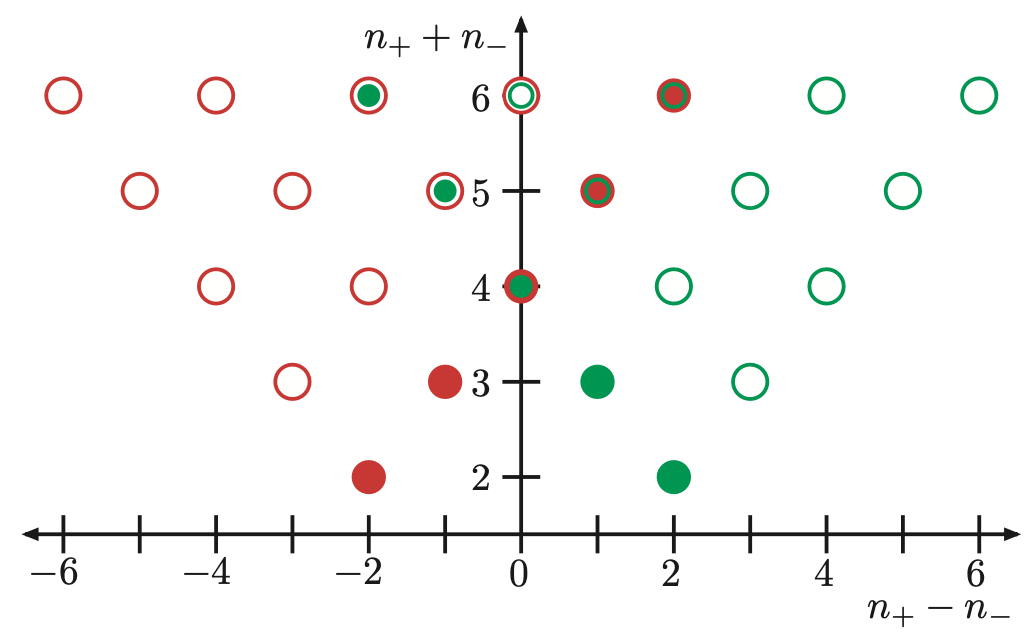
\includegraphics[width=0.4\textwidth]{MHVplot}
	\caption{Plot of number of gluons in terms of the difference in positive and negative helicity.}
\end{center}
\end{figure}
\fi
\iffalse
\begin{equation}
\begin{aligned}	
\tikzfeynmanset{ myblob/.style={ shape=circle, typeset=$nL$,
draw=black, } }
    \feynmandiagram [large, horizontal=b to c, baseline=(d.base)] {
      c -- [gluon] b [myblob, label={90:\(\text{\hspace{0.2cm}}\bullet\)}, label={70:\(\bullet\)}, label={30:\(\bullet\)}] -- [gluon] a,
      b -- [scalar] d [particle=\(H\)],
      f -- [gluon] b -- [white] e,
      g -- [gluon] b,
    };=
    \feynmandiagram [large, horizontal=b to c,  baseline=(d.base)] {
      c -- [gluon] b [myblob, label={90:\(\text{\hspace{0.2cm}}\bullet\)}, label={70:\(\bullet\)}, label={30:\(\bullet\)}] -- [gluon] a,
      b -- [scalar] d [particle=\(\phi\)],
      f -- [gluon] b -- [white] e,
      g -- [gluon] b,
    };+
    \feynmandiagram [large, horizontal=b to c,  baseline=(d.base)] {
      c -- [gluon] b [myblob, label={90:\(\text{\hspace{0.2cm}}\bullet\)}, label={70:\(\bullet\)}, label={30:\(\bullet\)}] -- [gluon] a,
      b -- [scalar] d [particle=\(\phi^\dagger\)],
      f -- [gluon] b -- [white] e,
      g -- [gluon] b,
    };
\end{aligned}
 \end{equation}
\begin{eqnarray*}
	\tikzfeynmanset{ my2blob/.style={ shape=circle, typeset=tree,
draw=black, } }
\begin{tikzpicture}[baseline=(current bounding box.center)]
  \begin{feynman}
    \diagram [horizontal=b to c] {
           b [my2blob] -- [gluon] a [particle=\(1^+\)], 
           b -- [gluon] w1 [particle=\(4^+\)],
      b  -- [scalar] d1 [particle=\(\phi\)],
      b -- [gluon] w2 [particle=\(2^+\)],
      b -- [gluon] d [ particle=\(3^+\)],
    };
  \end{feynman}
\end{tikzpicture}\scalebox{1.6}{$\stackrel{\text{on-shell}}{=}\,0$}
\end{eqnarray*}
\fi
%%%----Fine sezione
\section{One-loop all-plus $\phi$ amplitude}
We use the standard trace-based color decomposition with double traces at one-loop,
\begin{align}
	\mathcal{A}^{1L}(\phi;1,2,\dots,n)=g^nC\,c_\Gamma \sum_{c=1}^{\lfloor n/2 \rfloor+1} \sum_\sigma Gr_{n;c} A^{1L}_{n,c}\left(\phi;\sigma(1,2,\dots,n)\right).	\label{phidec1l}
\end{align}
where $\lfloor x \rfloor$ is the largest integer less than or equal to $x$ and $c_\Gamma$ is the standard loop factor. In the large $N_C$ limit the leading structure is
$$
	Gr_{n;1}(1)=N_C \Tr\left(T^{a_1}T^{a_2}\dots T^{a_n}\right),
$$
and we focus on the kinematical contribution attached to this color factor, $A^{1L}_{n,1}(\phi;1,\dots,n)$, which we will denote as $A^{1L}(\phi;1\dots, n)$.\\
The simplest one-loop partial amplitude describe the interaction between the $\phi$ field and all-plus gluons. The cut-constructible part is absent because any double cut requires the product of two trees and at least one of them vanishes due to (\ref{vanamp}). Then, this amplitude is purely rational. It was derived in \cite{Berger:2006sh} using recursion relations after an explicit computation in the case of two gluons,
\begin{align}
	A^{1L}(\phi;1^+,2^+,\dots n^+)=\frac{-2s_\phi^2}{\langle 12 \rangle \langle 23 \rangle \dots \langle n1 \rangle} =-2 A^{tree}(\phi^\dagger;1^+,2^+,\dots,n^+).	\label{1Lphi}
\end{align}
As already done for QCD amplitudes, we can separate the amplitude into contributions with different type of particles in the loop,
\begin{align}
	A^{1L}(\phi;1^+,2^+,\dots,n^+)=A^{1L[g]}+\frac{n_f}{N_C} A^{1L[f]}+\frac{n_s}{N_C} A^{1L[s]}=A^{1L[g-s]}+\left(\frac{d_s-2}{2}-\frac{n_f}{N_C}+\frac{n_s}{N_C}\right) A^{1L[s]}.
\end{align}
$A^{1L[g]}$ comes from gluon loops and the fermion contribution $A^{1L[f]}$ is opposite to the scalar one $A^{1L[s]}$. $A^{1L[g-s]}$ describes the difference between gluon and scalar effects.\\
Let us start considering the amplitude at the lowest multiplicity. The terms from fermion and scalar loops vanish and we have to compute only the gluon contribution,
\begin{align*}
	A^{1L}(\phi;1^+,2^+)=A^{1L[g]}=\left[
	\begin{aligned}
	\begin{tikzpicture}[scale=0.65,baseline=(current bounding box.center)]
 	 \begin{feynman}
    		\diagram [small, vertical=d to c] {
      			d2 [particle=\(\phi\)] -- [scalar] b -- [gluon] c
        			-- [gluon] d  -- [gluon] b,
      			d4 -- [gluon] c,
      			d -- [gluon] s ,
   		 };
  	\end{feynman}
	\end{tikzpicture}
	\end{aligned}+
	\begin{aligned}
	\begin{tikzpicture}[scale=0.65,baseline=(current bounding box.center)]
 	 \begin{feynman}
    		\diagram [small, horizontal=d2 to b] {
      			d2 [particle=\(\phi\)] -- [scalar] b -- [gluon, half right] c,
			c  -- [gluon, half right] b,
      			d4 -- [gluon] c,
      			c -- [gluon] s ,
   		 };
  	\end{feynman}
	\end{tikzpicture}
	\end{aligned}\right]=\frac{-2s_\phi^2}{\langle 12 \rangle \langle 21 \rangle}.
\end{align*}
The previous amplitude is the starting point of our recursion relation at one-loop level \cite{Bern_2005}. The computation is similar to the proof of MHV formula in section [\ref{MHVsection}]. We use the shift (\ref{shift}) and we observe that there is only a single contribution,
\begin{align*}
	A^{1L}(\phi;1^+,\dots,n^+)=A^{1L}(\phi;\hat 1^+,2^+,\dots, (n-1)^+, \hat P_{n-1,n}^+)\frac{1}{s_{n-1,n}} A^{tree}((n-1)^+,\hat n^+,(-\hat P_{n-1,n})^-),
\end{align*}
which shows the correctness of (\ref{1Lphi}).\\

Another rational set of one-loop $\phi$+gluon amplitudes is characterised by only one gluon with negative helicity \cite{Berger:2006sh}. The other $\phi$ amplitudes show discontinuities. For example we can see branch cuts studying the all-minus amplitude which was computed in \cite{Badger_2006}. 

\section{$\phi$ amplitudes with gluons and a quark-antiquark pair}
Another interesting set of amplitudes involves also a quark-antiquark pair. We will study pure QCD corrections to $\phi$+gluon amplitudes without considering quarks effects, but it is interesting to notice some properties if the theory has a couple of fermions.

These two partons do not interact directly with the self-dual Higgs. We have to consider at least an external gluon, indeed in the case of massless quarks $\mathcal{A}(\phi, 1_q, 2_{\bar q})$ vanishes due to angular momentum conservation.\\
At tree-level the $\phi$ amplitude with two quarks and all-plus gluons is zero,
\begin{align*}
	\mathcal{A}^{tree}(\phi,1_q^-, 2^+, \dots, j_{\bar q}^+,(j+1)^+, \dots, n^+)=0,
\end{align*}
and it is rational at one-loop \cite{Berger:2006sh}.

\chapter{Cut constructible pieces of the two-loop $\phi+4g^+$ amplitude}	\label{ch:cuts}
\section{Normalization of the color decomposition}
\iffalse
 we used the following color organization for one-loop amplitudes:
$$
	\mathcal{A}^{1L}(\phi;1,2,\dots,n)=g^nC\,c_\Gamma \sum_{c=1}^{\lfloor n/2 \rfloor+1} \sum_\sigma Gr_{n;c} A^{1L}_{n,c}\left(\phi;\sigma(1,2,\dots,n)\right).
$$
where $\lfloor x \rfloor$ is the largest integer less than or equal to $x$. The decomposition of the two-loop $\phi+$gluon amplitude 
will be
$$
	\mathcal{A}^{2L}(\phi,1,2,\dots,n)=g^{n+2} c_\Gamma^2 N_C \sum_{c=1}^{\lfloor n/2 \rfloor+1} \sum_\sigma Gr_{n;c} A^{2L}_{n,c}\left(\phi;\sigma(1,2,\dots,n)\right)
$$
Keeping in mind that
$$
	Gr_{n;1}(1)=N_C \Tr\left(T^{a_1}T^{a_2}\dots T^{a_n}\right),
$$
the unrenormalized amplitude
\fi
We consider the following decomposition of the two-loop $\phi+$gluon amplitude at leading color,
\begin{align}
	\mathcal{A}^{2L}(\phi,1,2,\dots,n)|_{\text{leading color}}=g^{n+2} c_\Gamma^2 N_C^2 C \sum_{\sigma\in S_n/C_n} \tr\left(T^{a_{\sigma(1)}}T^{a_{\sigma(2)}}\dots T^{a_{\sigma(n)}}\right)A^{2L}_{n,1}\left(\phi;\sigma(1,2,\dots,n)\right).	\label{Cgdec}
\end{align}
Due to the coupling between $\phi$ and gluons, we explicitly extracted the effective constant $C$ as already done at one-loop level (\ref{phidec1l}).\\
In this chapter, we will compute the cut-constructible pieces of $A^{2L}_{n,1}\left(\phi;1^+,2^+,3^+,4^+\right)$ which represent the main purpose of this project.
\section{Structure of the two-loop amplitude}
The unitarity condition of the S-matrix was expanded perturbatively in order to find the discontinuity of the two-loop amplitude (\ref{discamp}).\\
We observe the presence of double cuts in which we have to consider the product of two sub-amplitudes respectively at tree and one-loop level. In our case with one self-dual field, we can separate the double cuts into two sectors. In the first one, we will consider a tree-level YM vertex and a one-loop sub-amplitude involving $\phi$, while in the second sector we will study the contributions of double cuts with a pure gluon interaction at one-loop level and a tree $\phi$+gluon sub-amplitude. In order to obtain the discontinuity, we have to integrate over the two-particle phase-space
\begin{equation}
	\int \dd\Phi_2=\int \dd^4\ell_1 \dd^4\ell_2 \ \delta^{(+)}(\ell_1^2)\delta^{(+)}(\ell_1^2)\delta^{(4)}(\ell_2-\ell_1-P_a),	\label{phase-space}
\end{equation}
and we will describe this contributions in terms of scalar integrals.
In principle, at two-loop level we can also have contributions from three-particle cuts with tree-level sub-amplitudes. In the all-plus configuration, the three-particle cuts vanish, thanks to the behavior of tree-level amplitudes. We can consider the following helicity configuration of the three-particle cut in order to understand the absence of this contribution.
\begin{equation} 
\begin{aligned}	
\tikzfeynmanset{ myblob/.style={ shape=circle, typeset=$\bigcirc$,
draw=black, } }
\begin{tikzpicture}
  \begin{feynman}
    \diagram [horizontal=b to c] {
      b [blob,label={160:\(\bullet\)},label={180:\(\bullet\hspace{0.1cm}\)},label={200:\(\bullet\)},label={[red]85:\(\hspace{-0.2cm}-\)}, label={[violet]5:\(\hspace{-0.1cm}-\)}] --  [white] db -- [white] c [blob, label={-45:\(\bullet\)}, label={0:\(\hspace{0.1cm}\bullet\)}, label={-13:\(\hspace{0.04cm}\bullet\)},label={[red]90:\(+\)}, label={[violet]5:\(\hspace{-1.75cm}+\)}], %uso solo per distanziare i due blob, ma essendo bianchi verranno ricoperti
      b -- [white] ds -- [white] c,
      a [] -- [white] b
        -- [gluon, half left, out=60, in=120, red] c
        -- [gluon, half left, in=120, out=60] b ,
       b -- [gluon, violet] c,
      d1 [particle=\(+\)] -- [gluon] b,
      d3 [particle=\(+\)]-- [gluon] b,
      c -- [gluon] d4 [particle=\(+\)],
      c -- [gluon] d6 [particle=\(+\)],
      c -- [scalar] d [particle=\(\phi\)],
      c -- [white] d2 ,
    };

    %% Find the midpoint, which is halfway between b and c.
    \coordinate (midpoint) at ($(b)!0.5!(c)$);
    %% Draw a line starting 2 units above the midpoint, and ending 2 units below
    %% the midpoint.
    \draw [dashed] ($(midpoint) + (0, 2.1)$) -- ($(midpoint) + (0, -2.1)$);
  \end{feynman}
\end{tikzpicture}
\end{aligned}
\end{equation}
We have to consider at least two inner gluons with negative helicity to obtain a non-trivial result from the vertex which involves only gluons. This causes the vanishing behavior of the sub-amplitude with the self-dual Higgs, indeed $A^{tree}(\phi;+,+,\dots,+,\pm)=0$.\\
The absence of three-particle cuts shows that the reduction of the two-loop amplitude corresponds to a one-loop integral decomposition. Hence the discontinuities of the amplitude can be expressed in terms of scalar boxes, triangles and bubbles. The structure of the amplitude can be represented pictorially in the following way.
\begin{eqnarray*}
A^{2L}(\phi;1^+,2^+,3^+,4^+)\hspace{0.3cm}=&&\sum_i c_i\left[
\begin{tikzpicture}[scale=0.7,baseline=(current bounding box.center)]
  \begin{feynman}
  	\diagram [horizontal=b to d] {
      			a -- b
        			--  c
        			-- d --  a,
			d3  -- [] b,
			d2 -- [] b,
      			d1 -- [] a,
      			d4 -- [] c,
      			d -- [] s ,
   		 };
  \end{feynman}
\end{tikzpicture}\right]_i\\
&&\\
&&+\sum_i d_i \left[
\begin{tikzpicture}[scale=0.5,baseline=(current bounding box.center)]
 	 \begin{feynman}
    		\diagram [horizontal=s to d] {
      			d2 -- b -- c
        			-- d -- b,
      			d1 -- [] b,
			d3  -- [] c,
      			d4 -- [] c,
      			d -- [] s ,
   		 };
	\end{feynman}
\end{tikzpicture}
\right]_i+\sum_i d'_i \left[\begin{tikzpicture}[scale=0.65,baseline=(current bounding box.center)]
 	 \begin{feynman}
    		\diagram [vertical=c to d] {
      			d2 -- b --c
        			-- d --b,
      			d1 -- [] b,
			d3  -- [] b,
      			d4 -- [] c,
      			d -- [] s ,
   		 };
  	\end{feynman}
	\end{tikzpicture}\,\right]_i\\
	&&\\
&&+\sum_i e_i \left[\,
\begin{tikzpicture}[scale=0.7, transform shape, baseline=(current  bounding  box.center)]
     \begin{feynman}
    \vertex (x);
    \vertex[right=of x] (y);
    \vertex[above left=of x] (a);
    \vertex[below left=of x] (b);
    \vertex[above right=of y] (c);
    \vertex[below right=of y] (d);
    \vertex[right=of y] (e);
    \diagram*{
        (x) --[half left] (y),
        (x) --[half right] (y),
        (a) --(x),
        (x) -- (b),
        (y) --(c),
        (y) --(d),
        (y) -- (e),
    };
    \end{feynman}
    \end{tikzpicture}
\right]_i+\sum_i e'_i \left[
\begin{tikzpicture}[scale=0.7, transform shape, baseline=(current  bounding  box.center)]
     \begin{feynman}
    \vertex (x);
    \vertex[right=of x] (y);
    \path (x) ++ (180:1.5) node[vertex] (a);
    \path (y) ++ (-60:1.9) node[vertex] (b);
    \path (y) ++ (-30:1.9) node[vertex] (c);
    \path (y) ++ (30:1.9) node[vertex] (d);
    \path (y) ++ (60:1.9) node[vertex] (e);
    \diagram*{
        (x) --[half left] (y),
        (x) --[half right] (y),
        (a) --(x),
        (y.-60) -- (b),
        (y.-30) --(c),
        (y.30) --(d),
        (y.60) -- (e),
    };
    \end{feynman}
    \end{tikzpicture}
\right]_i\\
&&\\
&&+\big[(d=4-2\epsilon) \text{ finite contributions}\big] + \mathcal{O}(\epsilon)
\end{eqnarray*}
Besides contributions proportional to the scalar integrals, in the amplitude we also have an effect due to the dimensional regularisation which can produce a finite contribution without discontinuities.\\%The expectation is that also in our case of a two-loop amplitude with the simplest helicity configuration, this missing information from unitarity-based techniques is rational.\\
In this chapter, we will isolate the coefficients of scalar integrals, separating the discontinuities into two sectors with different perturbative levels of YM and self-dual Higgs sub-amplitudes.
\section{Double cuts with 1L $\phi$ amplitudes and tree YM amplitudes} \label{sec:cutphi}
In this section, we study the double cuts which factorize into the product of a one-loop $\phi+$gluon amplitude and a tree level gluon amplitude. Preliminarily, we have computed the quadruple cuts in order to isolate and extract the contributions proportional to the four-point integrals using simple calculations (see Appendix \ref{appC}). Computing the double cuts, we will find all the discontinuities of the amplitude. We will compare the box contributions obtained with the two independent computations in order to have a partial check for the correctness of double cuts.\\
We have to compute three different double cuts to capture the discontinuities in the three channels $s_\phi, s_{\phi1}, s_{34}$.\\
\vspace{-0.2cm}
\noindent
\begin{tabularx}{\linewidth}{XX}
\begin{equation}  \tag{dcut A}
    \begin{aligned}	\label{dcut A}
\tikzfeynmanset{ myblob/.style={ shape=circle, typeset=$\bigcirc$,
draw=black, } }
\begin{tikzpicture}
  \begin{feynman}
    \diagram [scale=0.95, large, horizontal=b to c] {
      b [blob] --  [white] db -- [white] c [myblob], %uso solo per distanziare i due blob, ma essendo bianchi verranno ricoperti
      b -- [white] ds -- [white] c,
      a [particle=\(4^+\)] -- [gluon] b
        -- [gluon, half left, out=60, in=120, momentum=\(\ell_1\)] c
        -- [gluon, half left, in=120, out=60, momentum=\(\ell_2\)] b ,
      d1 [particle=\(1^+\)] -- [gluon] b,
      d2 [particle=\(3^+\)] -- [gluon] b,
      d3 [particle=\(2^+\)]-- [gluon] b,
      c -- [scalar] d [particle=\(\phi\)],
    };

    %% Find the midpoint, which is halfway between b and c.
    \coordinate (midpoint) at ($(b)!0.5!(c)$);
    %% Draw a line starting 2 units above the midpoint, and ending 2 units below
    %% the midpoint.
    \draw [dashed] ($(midpoint) + (0, 2.2)$) -- ($(midpoint) + (0, -2.2)$);
  \end{feynman}
\end{tikzpicture}
\end{aligned}
\end{equation}
&
\vspace{-0.2cm}
\begin{equation} \tag{dcut B}
    \begin{aligned}	\label{dcut B}
\tikzfeynmanset{ myblob/.style={ shape=circle, typeset=$\bigcirc$,
draw=black, } }
\begin{tikzpicture}
  \begin{feynman}
    \diagram [large, horizontal=b to c] {
      b [blob] --  [white] db -- [white] c [myblob], %uso solo per distanziare i due blob, ma essendo bianchi verranno ricoperti
      b -- [white] ds -- [white] c,
      a [particle=\(4^+\)] -- [gluon] b
        -- [gluon, half left, out=60, in=120, momentum=\(\ell_1\)] c
        -- [gluon, half left, in=120, out=60, momentum=\(\ell_2\)] b ,
      d1 [particle=\(2^+\)] -- [gluon] b,
      d3 [particle=\(3^+\)]-- [gluon] b,
      c -- [scalar] d [particle=\(\phi\)],
      c -- [gluon] d2 [particle=\(1^+\)],
    };

    %% Find the midpoint, which is halfway between b and c.
    \coordinate (midpoint) at ($(b)!0.5!(c)$);
    %% Draw a line starting 2 units above the midpoint, and ending 2 units below
    %% the midpoint.
    \draw [dashed] ($(midpoint) + (0, 2.1)$) -- ($(midpoint) + (0, -2.1)$);
  \end{feynman}
\end{tikzpicture}
\end{aligned}
\end{equation}
\end{tabularx}

\vspace{-2.1cm}
\newcolumntype{b}{>{\hsize=2.3\hsize}X}
\newcolumntype{s}{>{\hsize=.45\hsize}X}
\begin{tabularx}{\textwidth}{sbs}
&
 \begin{equation} \tag{dcut C}
\text{\hspace{1.1cm}}\,\,
\begin{aligned}	\label{dcut C}
\tikzfeynmanset{ myblob/.style={ shape=circle, typeset=$\bigcirc$,
draw=black, } }
\begin{tikzpicture}
  \begin{feynman}
    \diagram [scale=1, transform shape, large, horizontal=b to c] {
      b [blob] --  [white] db -- [white] c [myblob], %uso solo per distanziare i due blob, ma essendo bianchi verranno ricoperti
      b -- [white] ds -- [white] c,
      a [particle=\(4^+\)] -- [gluon] b
        -- [gluon, half left, out=60, in=120, momentum=\(\ell_1\)] c
        -- [gluon, half left, in=120, out=60, momentum=\(\ell_2\)] b ,
      d1 [particle=\(3^+\)] -- [gluon] b,
      c -- [scalar] d [particle=\(\phi\)],
      c -- [gluon] d3 [particle=\(1^+\)],
      c -- [gluon] d2 [particle=\(2^+\)],
    };

    %% Find the midpoint, which is halfway between b and c.
    \coordinate (midpoint) at ($(b)!0.5!(c)$);
    %% Draw a line starting 2 units above the midpoint, and ending 2 units below
    %% the midpoint.
    \draw [dashed] ($(midpoint) + (0, 1.5)$) -- ($(midpoint) + (0, -1.5)$);
  \end{feynman}
\end{tikzpicture}
\end{aligned}
 \end{equation} &
 \end{tabularx}
Due to the colorless of the self-dual Higgs, we are also interested in configurations obtained through a cyclic permutation of gluons. The last possible channel with a different structure is characterised by a single external gluon (for example, the fourth gluon) on the left-hand side and it does not contribute to the discontinuities of the amplitude (indeed $s_4$ vanishes).\\
We have considered only gluons circulating in the loop since we want to extract two-loop QCD corrections. Furthermore, the other possible particles in our model, the complex scalars $\phi$ and $\phi^\dagger$, can be coupled in a diagram only through an effective vertex with coupling $C$. Considering $C$ and $g$ as independent parameters, the double cuts with inner scalar legs will be associated to a different amplitude in comparison with (\ref{Cgdec}) which is proportional to $Cg^{n+2}$.\\%\footnote{Since in the SM the effective interaction implies a quark loop, double cuts of a gluon and a scalar field have the same perturbative order of our amplitude if we consider tree-level sub-amplitudes.  These scalar contributions should be useful for the renormalisation of the Wilson coefficient, but they affect a different type of amplitude. For this reason, we focus on the double cuts with only inner gluon propagators because they represent the full contribution for the discontinuities of (\ref{Cgdec}).}\\

In each double cut, we will reduce the product of the sub-amplitudes in terms of scalar integrals considering the possible helicity configuration of the inner gluons. With these computations, we will extract the coefficients of boxes, triangles and bubbles which characterised the discontinuities of the two-loop amplitude in this sector with a one-loop $\phi$+gluon sub-amplitude.
\subsection{Double cut in $s_{\phi}$ channel}
Let us study the double cut represented by the diagram (\ref{dcut A}). In order to evaluate the double cut, we have to compute the following object,
\begin{align*}
	A^{2L}_{int}|_{\text{dcut A}}&=\sum_{\lambda_1=\pm}\sum_{\lambda_2=\pm}A^{tree}(1^+,2^+,3^+,4^+,\ell_1^{\lambda_1},(-\ell_2)^{\lambda_2})A^{1L}(\phi;\ell_2^{-\lambda_2},(-\ell_1)^{-\lambda_1})\\
	&=A^{tree}(1^+,2^+,3^+,4^+,\ell_1^{-},(-\ell_2)^{-})A^{1L}(\phi;\ell_2^{+},(-\ell_1)^{+})\\
	&=A^{1L}(\phi;1^+,2^+,3^+,4^+)\frac{\langle \ell_1\ell_2\rangle \langle 41 \rangle}{\langle \ell_2 1\rangle \langle \ell_1 4\rangle}.
\end{align*}
We reconstruct the propagators at the denominator intending to write it in terms of scalar integrals,
\begin{align*}
	\frac{A^{2L}_{int}|_{\text{dcut A}}}{A^{1L}(\phi;1^+,2^+,3^+,4^+)}&=\frac{\langle \ell_1\ell_2\rangle \langle 41 \rangle}{\langle \ell_2 1\rangle \langle \ell_1 4\rangle}=\frac{-\frac{1}{2}\tr(\slashed{p}_1\slashed{p}_4\slashed{\ell}_1\slashed{\ell}_2)-\frac{1}{2}\tr_5(p_1{p}_4{\ell}_1{\ell}_2)}{(\ell_2-p_1)^2(\ell_1+p_4)^2}.
\end{align*}
Let us focus our attention on the term with $\tr_5$,
\begin{align}
	\frac{\tr_5({p}_1{p}_4{\ell}_1{\ell}_2)}{(\ell_2-p_1)^2(\ell_1+p_4)^2}&=\frac{\tr_5({p}_1{p}_4{\ell}_1{P}_a)}{(\ell_1+P-p_1)^2(\ell_1+p_4)^2} \label{eq:dcuttr5}
\end{align}
where we introduce the momentum $P_a=p_1+p_2+p_3+p_4=-p_\phi$.\\
The unitarity procedure requires the integration over the phase-space (\ref{phase-space}). Then we can perform the substitution $\ell_1\rightarrow -\ell_1-p_4-P_a+p_1$ in the integrand (\ref{eq:dcuttr5}). Using the antisymmetry property of $\gamma_5$, we obtain
\begin{align*}
	\int \dd\Phi_2 \frac{\tr_5({p}_1{p}_4{\ell}_1{\ell}_2)}{(\ell_2-p_1)^2(\ell_1+p_4)^2}&= \int \dd\Phi_2  \frac{\tr_5({p}_1{p}_4(-{\ell}_1-p_4-P_a+p_1){P}_a)}{(-\ell_1-p_4)^2(-\ell_1-P_a+p_1)^2}\\
	&=\int \dd\Phi_2  \frac{-\tr_5({p}_1{p}_4{\ell}_1{P}_a)}{(\ell_1+p_4)^2(\ell_1+P_a-p_1)^2}=- \int \dd\Phi_2 \frac{\tr_5({p}_1{p}_4{\ell}_1{\ell}_2)}{(\ell_2-p_1)^2(\ell_1+p_4)^2}.
\end{align*}
This computation shows that the $\tr_5$ contribution represents a spurious term. We are left with the following contribution,
\begin{align*}
	\frac{A^{2L}_{int}|_{\text{dcut A}}}{A^{1L}(\phi;1^+,2^+,3^+,4^+)}
	%&=\frac{-\frac{1}{2}\tr(\slashed{p}_1\slashed{p}_4\slashed{\ell}_1\slashed{\ell}_2)}{(\ell_2-p_1)^2(\ell_1+p_4)^2}+\text{s.t.}=\frac{-\frac{1}{2}\tr(\slashed{p}_1\slashed{p}_4\slashed{\ell}_1\slashed{P}_a)}{(\ell_2-p_1)^2(\ell_1+p_4)^2}+\text{s.t.}=\\
%	&=-\frac{2(p_1\cdot p_4)(\ell_1\cdot P_a)-2(p_1\cdot \ell_1)(p_4 \cdot P_a)+2(p_4\cdot \ell_1)(p_1 \cdot P_a)}{(\ell_2-p_1)^2(\ell_1+p_4)^2}+\text{s.t.}\\
%	&=-\frac{(p_1\cdot p_4)(\ell_2^2-P_a^2)-2(p_1\cdot \ell_2-p_1\cdot P_a)(p_4 \cdot P_a)+2(p_4\cdot \ell_1)(p_1 \cdot P_a)}{(\ell_2-p_1)^2(\ell_1+p_4)^2}+\text{s.t.}\\
	&=\frac{(p_1\cdot p_4)P_a^2-2(p_1\cdot P_a)(p_4\cdot P_a)}{(\ell_2-p_1)^2(\ell_1+p_4)^2}-\frac{p_4\cdot P_a}{(\ell_1+p_4)^2}-\frac{p_1\cdot P_a}{(\ell_2-p_1)^2}+\text{s.t.}
\end{align*}
where $"\text{s.t.}"$ implies the presence of spurious terms which vanish after the phase-space integration.\newpage
We represent the result diagrammatically
\begin{eqnarray*}	
&&\tikzfeynmanset{ myblob/.style={ shape=circle, typeset=$\bigcirc$,
draw=black, } }
\begin{tikzpicture}[baseline=(current bounding box.center)]
  \begin{feynman}
    \diagram [baseline=(b.base),horizontal=b to c] {
      b [blob] --  [white] db -- [white] c [myblob], %uso solo per distanziare i due blob, ma essendo bianchi verranno ricoperti
      b -- [white] ds -- [white] c,
      a [particle=\(2^+\)] -- [gluon] b
        -- [gluon, half left, out=60, in=120, momentum=\(\ell_1\)] c
        -- [gluon, half left, in=120, out=60, momentum=\(\ell_2\)] b ,
      d1 [particle=\(3^+\)] -- [gluon] b,
      d2 [particle=\(1^+\)] -- [gluon] b,
      d3 [particle=\(4^+\)]-- [gluon] b,
      c -- [scalar] d [particle=\(\phi\)],
    };

    %% Find the midpoint, which is halfway between b and c.
    \coordinate (midpoint) at ($(b)!0.5!(c)$);
    %% Draw a line starting 2 units above the midpoint, and ending 2 units below
    %% the midpoint.
    \draw [dashed] ($(midpoint) + (0, 1.5)$) -- ($(midpoint) + (0, -1.5)$);
  \end{feynman}
\end{tikzpicture}
\rightarrow C^A_4	\left[
         \begin{tikzpicture}[baseline=(current bounding box.center)]
 	 \begin{feynman}
    		\diagram [horizontal=b to d] {
      			a -- [momentum={\tiny\(\ell_2-p_1\)}] b
        			-- [momentum={\tiny\(\ell_1+p_4\)}] c
        			-- [momentum={\tiny\(\ell_1\)}] d -- [momentum={\tiny\(\ell_2\)}] a,
			d3  [particle=\(3\)]-- [] b,
			d2 [particle=\(2\)]-- [] b,
      			d1 [particle=\(1\)]-- [] a,
      			d4 [particle=\(4\)]-- [] c,
      			d -- [] s [particle=\(\phi\)],
   		 };
    		\coordinate (midpoint) at ($(b)!0.75!(d)$);
   		\draw [dashed] ($(midpoint) + (0, 1.5)$) -- ($(midpoint) + (0, -1.5)$);
  	\end{feynman}
	\end{tikzpicture}
	\right]+\\
	&&\hspace{2.5cm}
	+ C^A_{3,1} \left[
	\begin{tikzpicture}[baseline=(current bounding box.center)]
 	 \begin{feynman}
    		\diagram [vertical=c to d] {
      			d2 [particle=\(4\)]-- b -- [momentum={\tiny\(\ell_1\)}] c
        			-- [momentum={\tiny\(\ell_2\)}] d -- [momentum={[label distance=-3.5pt]\tiny\(\ell_2-p_1\)}] b,
      			d1 [particle=\(3\)]-- [] b,
			d3  [particle=\(2\)]-- [] b,
      			d4 [particle=\(\phi\)]-- [] c,
      			d -- [] s [particle=\(1\)],
   		 };
    		\coordinate (midpoint) at ($(b)!0.5!(d)$);
		\coordinate (midpoint2) at ($(c)!0.5!(d)$);
   		\draw [dashed] ($(midpoint2) + (1, -0.25)$) to[out=180, in=-90] ($(midpoint) + (-0.25, 1.75)$);
  	\end{feynman}
	\end{tikzpicture}	\right]
	+ C^A_{3,2} \left[
	\begin{tikzpicture}[baseline=(current bounding box.center)]
 	 \begin{feynman}
    		\diagram [vertical=c to d] {
      			d2 [particle=\(3\)]-- b -- [momentum={[label distance=-3.5pt]\tiny\(\ell_1+p_4\)}] c
        			-- [momentum={\tiny\(\ell_1\)}] d -- [momentum={\tiny\(\ell_2\)}] b,
      			d1 [particle=\(2\)]-- [] b,
			d3  [particle=\(1\)]-- [] b,
      			d4 [particle=\(4\)]-- [] c,
      			d -- [] s [particle=\(\phi\)],
   		 };
    		\coordinate (midpoint) at ($(b)!0.5!(d)$);
		\coordinate (midpoint2) at ($(c)!0.5!(d)$);
   		\draw [dashed] ($(midpoint2) + (1, 0.25)$) to[out=180, in=90] ($(midpoint) + (-0.25, -1.15)$);
  	\end{feynman}
	\end{tikzpicture}\right]
 \end{eqnarray*}
 where the coefficients in front of scalar integrals are
 \begin{align*}
 	C^A_4&\coloneqq A^{1L}(\phi;1^+,2^+,3^+,4^+)\left[(p_1\cdot p_4) P_a^2-2(p_1\cdot P) (p_4 \cdot P_a)\right]\\
	&=\frac{1}{2}A^{1L}(\phi;1^+,2^+,3^+,4^+)\left[s_{14}s_{\phi}-(s_{1\phi}-s_{\phi})(s_{\phi4}-s_\phi)\right]\\
	C^A_{3,1}&\coloneqq A^{1L}(\phi;1^+,2^+,3^+,4^+)\left[-p_1\cdot P_a\right]=\frac{1}{2}(s_{\phi1}-s_\phi)A^{1L}(\phi;1^+,2^+,3^+,4^+)\\
	C^A_{3,2}&\coloneqq A^{1L}(\phi;1^+,2^+,3^+,4^+)\left[-p_4\cdot P_a\right]=\frac{1}{2}(s_{4\phi}-s_\phi)A^{1L}(\phi;1^+,2^+,3^+,4^+).
 \end{align*}
 In a more compact form, we have
 \begin{align*}
 	A^{2L}|_{\text{dcut A}}\equiv\int \dd \Phi_2 \ A^{2L}_{int}|_{\text{dcut A}}=&C^A_4 \left.I_4^{2me}(s_{\phi4},s_{1\phi};m_1^2=s_{23},m_2^2=s_\phi)\right|_{s_{\phi}\text{-cut}}\\
	&+C^A_{3,1}I_3^{2m}(s_{1\phi},s_\phi)|_{s_{\phi}\text{-cut}}+C^A_{3,2}I_3^{2m}(s_{\phi4},s_\phi)|_{s_{\phi}\text{-cut}}
 \end{align*}
where we have introduced the easy two-mass box and the three-point integral with two massive vertices whose expressions can be found in App. [\ref{appB}].\\
 %$$
 %	I_3^{2m}(m_1^2,m_2^2)=\frac{1}{\epsilon^2}\frac{\left(-m_1^2\right)^{-\epsilon}-\left(-m_2^2\right)^{-\epsilon}}{(-m_1^2)-(-m_2^2)}.
 %$$
% As expected from quadruple cuts, we did not find in the $s_\phi$ channel a contribution proportional to the hard two-mass box and we can check the correctness of the coefficient in front of the easy two-mass four-point integral using the property $P_a=-p_{\phi}$:
%\begin{align*}
%	C^A_4&=A^{1L}(\phi;1^+,2^+,3^+,4^+)\left[(p_1\cdot p_4) P^2-2(p_1\cdot P) (p_4 \cdot P)\right]\\
%	&=A^{1L}(\phi;1^+,2^+,3^+,4^+)\left[\frac{1}{2}s_{14}s_\phi-2(p_1\cdot p_\phi)(p_4 \cdot p_\phi)\right]\\
%	&=\frac{1}{2}A^{1L}(\phi;1^+,2^+,3^+,4^+)\left[s_{14}s_{\phi}-(s_{1\phi}-s_{\phi})(s_{\phi4}-s_\phi)\right]=d_1^{(2me)}.
%\end{align*}
The coefficient $C^A_4$ is consistent with the result from quadruple cuts (\ref{eq:2meboxcoef}).
Investigating the amplitude using the double cut, we were able to extract more information: we obtained the coefficients of three-point two-mass integrals and the absence of other triangles or bubbles.
\subsection{Double cut in $s_{\phi1}$ channel}	\label{sec:dcutB}
The next double cut concerns the $s_{\phi1}$ channel (\ref{dcut B}).
The discontinuities along this channel are related to the phase-space integration of the following quantity.
\begin{align*}
	A^{2L}_{int}|_{\text{dcut B}}&=\sum_{\lambda_1=\pm}\sum_{\lambda_2=\pm}A^{tree}(2^+,3^+,4^+,\ell_1^{\lambda_1},(-\ell_2)^{\lambda_2})A^{1L}(\phi;1^+,\ell_2^{-\lambda_2},(-\ell_1)^{-\lambda_1})\\
	&=A^{tree}(2^+,3^+,4^+,\ell_1^{-},(-\ell_2)^{-})A^{1L}(\phi;1^+,\ell_2^{+},(-\ell_1)^{+})\\
	&=\frac{-2m_H^4}{\langle 23 \rangle\langle 34 \rangle}\frac{\langle \ell_1\ell_2 \rangle^2}{\langle 1 \ell_1 \rangle \langle 1 \ell_2 \rangle \langle 2 \ell_2 \rangle\langle 4 \ell_1 \rangle}
\end{align*}
In this step of the calculation, we find the Schouten identity very useful in reducing the complexity of the object.
%We can rewrite this property in the following way:
%$$
%	\frac{\langle \lambda a \rangle}{\langle \lambda b \rangle \langle \lambda c \rangle}=\frac{\langle ba \rangle}{\langle bc \rangle \langle \lambda b \rangle}+\frac{\langle ac \rangle}{\langle bc\rangle\langle \lambda c \rangle}
%$$
In our case we apply the substitution
\begin{align*}
	\frac{\langle\ell_1 \ell_2 \rangle}{\langle 1\ell_1 \rangle \langle 4\ell_1 \rangle}&=\frac{1}{\langle 14 \rangle}\left(\frac{\langle 1 \ell_2 \rangle}{\langle \ell_1 1\rangle}+\frac{\langle \ell_2 4 \rangle}{\langle \ell_1 4 \rangle}\right).
\end{align*}
and a similar expression holds for the reduction of spinors with $\ell_2$ at denominator. We obtain
\begin{align*}
	A^{2L}_{int}|_{\text{dcut B}}&=A^{1L}(\phi;1^+,2^+,3^+,4^+)(-1+\Sigma_1+\Sigma_2+\Sigma_3)
\end{align*}
where
\begin{align*}
	\Sigma_1\coloneqq\frac{\langle 1 \ell_1 \rangle \langle 4\ell_2 \rangle}{\langle \ell_2 1 \rangle \langle \ell_1 4 \rangle},\ \ \ \ \Sigma_2\coloneqq\frac{\langle \ell_1 2 \rangle \langle \ell_2 1 \rangle}{\langle \ell_2 2 \rangle \langle \ell_1 1 \rangle},\ \ \ \ \Sigma_3\coloneqq\frac{\langle \ell_1 2 \rangle \langle 4 \ell_2 \rangle}{\langle \ell_2 2 \rangle\langle \ell_1 4 \rangle}.
\end{align*}
We can easily simplify every addend reconstructing the propagators at the denominator. For example, let us focus on the term
$$
	 \Sigma_1=\frac{\langle 1 \ell_1 4] \langle 4 \ell_2 1]}{\langle 1 \ell_2 1]\langle 4 \ell_14]}=\frac{\tr_-\left({p}_1{\ell}_1{p}_4{\ell}_2\right)}{(\ell_2+p_1)^2(\ell_1+p_4)^2}.
$$
Avoiding terms which vanish after the integration, we obtain
\begin{align*}
	\Sigma_1&=1-\frac{\frac{1}{2}\tr\left(\slashed{p}_1\slashed{p}_4\slashed{\ell}_1\slashed{\ell}_2\right)}{(\ell_2+p_1)^2(\ell_1+p_4)^2}+\text{s.t.}=1-\frac{\frac{1}{2}\tr\left(\slashed{p}_1\slashed{p}_4\slashed{\ell}_1\slashed{P}_b\right)}{(\ell_2+p_1)^2(\ell_1+p_4)^2}+\text{s.t.}
\end{align*}
where in the last passage we introduced $P_b=p_2+p_3+p_4=-p_1-p_\phi$ and we used the on-shell condition $\ell_2^2=0$. 
Expanding the trace of four Gamma matrices, we have
$$
	\Sigma_1=1-\frac{2(p_1\cdot P_b)(p_4 \cdot P_b)-(p_1\cdotp_4)P_b^2}{(\ell_2+p_1)^2(\ell_1+p_4)^2}+\frac{p_4\cdot P_b}{(\ell_1+p_4)^2}-\frac{p_1\cdot P_b}{(\ell_2+p_1)^2}+\text{s.t.}.
$$
Similarly, one can compute the other two addends,
\begin{align*}
	\Sigma_2&=1-\frac{2(p_2\cdot P_b)(p_1 \cdot P_b)-(p_1\cdot p_2)P_b^2}{(\ell_2-p_2)^2(\ell_1-p_1)^2}-\frac{p_1\cdot P_b}{(\ell_1-p_1)^2}+\frac{p_2\cdot P_b}{(\ell_2-p_2)^2}+\text{s.t.},\\
	\Sigma_3&=-1-\frac{2(p_2\cdot P_b)(p_4 \cdot P_b)-(p_2\cdot p_4)P_b^2}{(\ell_2-p_2)^2(\ell_1+p_4)^2}-\frac{p_4\cdot P_b}{(\ell_1+p_4)^2}-\frac{p_2\cdot P_b}{(\ell_2-p_2)^2}+\text{s.t.}
\end{align*}
Summing the contributions, we find
\begin{align*}
	A^{2L}|_{\text{dcut B}}\int \dd \Phi_2 A^{2L}_{int}|_{\text{dcut B}}=&C^B_{4,1} I_4^{2me}(s_{\phi4},s_{1\phi};s_{23},s_\phi)|_{s_{\phi1}\text{-cut}}+C^B_{4,2} I_4^{2me}(s_{1\phi},s_{\phi2};s_{34},s_\phi)|_{s_{\phi1}\text{-cut}}+\\
	&C^B_{4,3} I_4^{1m}(s_{23},s_{34};s_{1\phi})|_{s_{\phi1}\text{-cut}}+2C^B_{3} I_3^{2m}(s_{1\phi},s_\phi)|_{s_{\phi1}\text{-cut}}	\numthis \label{eq:risdcB}
\end{align*}
with the coefficients
\begin{align*}
	C^B_{4,1}&\coloneqq \frac{1}{2}A^{1L}(\phi;1^+,2^+,3^+,4^+)\left[s_{14}s_{\phi}-(s_{1\phi}-s_\phi)(s_{4\phi}-s_{\phi})\right],\\
	C^B_{4,2}&\coloneqq \frac{1}{2}A^{1L}(\phi;1^+,2^+,3^+,4^+)\left[s_{12}s_{\phi}-(s_{1\phi}-s_\phi)(s_{2\phi}-s_{\phi})\right],\\
	C^B_{4,3}&\coloneqq -\frac{1}{2}s_{23}s_{34}A^{1L}(\phi;1^+,2^+,3^+,4^+),\\
	C^B_{3}&\coloneqq A^{1L}(\phi;1^+,2^+,3^+,4^+)\left[-p_1\cdot P_b\right]=\frac{1}{2}(s_{\phi1}-s_{\phi})A^{1L}(\phi;1^+,2^+,3^+,4^+).
\end{align*}
We have two easy boxes with only a different organization of legs. Indeed $\phi$ is unordered, therefore investigating the $s_{\phi1}$ channel we find two four-point contributions with different orders, but with the same relative positions between gluons.
\begin{eqnarray*}
	 I_4^{2me}(s_{\phi4},s_{1\phi};s_{23},s_\phi)|_{s_{\phi1}\text{-cut}}=
	 \begin{tikzpicture}[baseline=(current bounding box.center)]
 	 \begin{feynman}
    		\diagram [horizontal=b to d] {
      			a -- [momentum={\tiny\(\ell_2\)}] b
        			-- [momentum={\tiny\(\ell_1+p_4\)}] c
        			-- [momentum={\tiny\(\ell_1\)}] d -- [momentum={\tiny\(\ell_2+p_1\)}] a,
			d3  [particle=\(3\)]-- [] b,
			d2 [particle=\(2\)]-- [] b,
      			d1 [particle=\(1\)]-- [] a,
      			d4 [particle=\(4\)]-- [] c,
      			d -- [] s [particle=\(\phi\)],
   		 };
    		\coordinate (midpoint) at ($(b)!0.75!(d)$);
   		\draw [dashed] ($(midpoint) + (0.75, 1.35)$) -- ($(midpoint) + (-1.6, -1.3)$);
  	\end{feynman}
	\end{tikzpicture}
	\\
	I_4^{2me}(s_{1\phi},s_{\phi2};s_{34},s_\phi)|_{s_{\phi1}\text{-cut}}=
	 \begin{tikzpicture}[baseline=(current bounding box.center)]
 	 \begin{feynman}
    		\diagram [horizontal=b to d] {
      			a -- [momentum={\tiny\(\ell_2-p_2\)}] b
        			-- [momentum={\tiny\(\ell_1\)}] c
        			-- [momentum={\tiny\(\ell_1-p_1\)}] d -- [momentum={\tiny\(\ell_2\)}] a,
			d3  [particle=\(4\)]-- [] b,
			d2 [particle=\(3\)]-- [] b,
      			d1 [particle=\(2\)]-- [] a,
      			d4 [particle=\(1\)]-- [] c,
      			d -- [] s [particle=\(\phi\)],
   		 };
    		\coordinate (midpoint) at ($(b)!0.75!(d)$);
   		\draw [dashed] ($(midpoint) + (0.75, -1.3)$) -- ($(midpoint) + (-1.6, 1.2)$);
  	\end{feynman}
	\end{tikzpicture}
\end{eqnarray*}
The coefficients $C^B_{4,1}$ and $C^B_{4,2}$ are consistent with the results from quadruple cuts (\ref{eq:2meboxcoef}).\\
In this cut, we also observe the presence of a contribution proportional to the one-mass box
$$
	 I_4^{1m}(s_{23},s_{34};s_{1\phi})|_{s_{\phi1}\text{-cut}}=
	 \begin{tikzpicture}[baseline=(current bounding box.center)]
 	 \begin{feynman}
    		\diagram [horizontal=b to d] {
      			a -- [momentum={\tiny\(\ell_1\)}] b
        			-- [momentum={\tiny\(\ell_2\)}] c
        			-- [momentum={\tiny\(\ell_2-p_2\)}] d -- [momentum={\tiny\(\ell_1+p_4\)}] a,
			d3  [particle=\(1\)]-- [] b,
			d2 [particle=\(\phi\)]-- [] b,
      			d1 [particle=\(4\)]-- [] a,
      			d4 [particle=\(2\)]-- [] c,
      			d -- [] s [particle=\(3\)],
   		 };
    		\coordinate (midpoint) at ($(b)!0.25!(d)$);
   		\draw [dashed] ($(midpoint) + (0, -1.5)$) -- ($(midpoint) + (0, 1.5)$);
  	\end{feynman}
	\end{tikzpicture}
$$
which cannot be seen studying the double cut in the $s_\phi$ channel. The coefficient corresponds to the result (\ref{eq:d11m}) from the quadruple cut for the one-mass box.\\

From the double cuts we are able to extract information about triangles and bubbles. We observe that the only non-vanishing three-point contribution in this channel is $I_3^{2m}(s_{1\phi},s_\phi)$ which comes from the following two diagrams.
$$
	\begin{tikzpicture}[baseline=(current bounding box.center)]
 	 \begin{feynman}
    		\diagram [scale=0.9,vertical=c to d] {
      			d2 [particle=\(4\)]-- b -- [momentum={\tiny\(\ell_1\)}] c
        			-- [momentum={\tiny\(\ell_2+p_1\)}] d -- [momentum={\tiny\(\ell_2\)}] b,
      			d1 [particle=\(3\)]-- [] b,
			d3  [particle=\(2\)]-- [] b,
      			d4 [particle=\(\phi\)]-- [] c,
      			d -- [] s [particle=\(1\)],
   		 };
    		\coordinate (midpoint) at ($(b)!0.5!(d)$);
   		\draw [dashed] ($(midpoint) + (0, -1.25)$) to($(midpoint) + (0, 1.75)$);
  	\end{feynman}
	\end{tikzpicture}
	\hspace{1cm}
	\begin{tikzpicture}[baseline=(current bounding box.center)]
 	 \begin{feynman}
    		\diagram [scale=0.9,vertical=c to d] {
      			d2 [particle=\(4\)]-- b -- [momentum={\tiny\(\ell_1\)}] c
        			-- [momentum={\tiny\(\ell_1-p_1\)}] d -- [momentum={\tiny\(\ell_2\)}] b,
      			d1 [particle=\(3\)]-- [] b,
			d3  [particle=\(2\)]-- [] b,
      			d4 [particle=\(1\)]-- [] c,
      			d -- [] s [particle=\(\phi\)],
   		 };
    		\coordinate (midpoint) at ($(b)!0.5!(d)$);
   		\draw [dashed] ($(midpoint) + (0, -1.25)$) to($(midpoint) + (0, 1.75)$);
  	\end{feynman}
	\end{tikzpicture}
$$
These two equivalent contributions proportional to the three-point integral are related to the switch of the legs $\phi$ and $1$. Although the topology of these contributions is not the same, the scalar integrals can be mapped in each other through a simple change of variables: for this reason, we collect together the two objects.\\
Obviously the other triangle $I_3^{2m}(s_{4\phi},s_\phi)$, detected using the first double cut, cannot be obtained in the $s_{\phi1}$ channel. However, using the present double cut, we could expect other three-point contributions, for example in the intermediate steps we observe the presence of terms like the following which emerges in $\Sigma_1$,
\begin{eqnarray*}
	\frac{p_4\cdot P_b}{(\ell_1+p_4)^2} \rightarrow (p_4\cdot P_b)\left[
	\begin{tikzpicture}[baseline=(current bounding box.center)]
 	 \begin{feynman}
    		\diagram [scale=0.7,horizontal=s to d] {
      			d2 [particle=\(\phi\)]-- b -- [momentum={\tiny\(\ell_1\)}] c
        			-- [momentum={\tiny\(\ell_1-p_1\)}] d -- [momentum={\tiny\(\ell_2\)}] b,
      			d1 [particle=\(1\)]-- [] b,
			d3  [particle=\(2\)]-- [] c,
      			d4 [particle=\(3\)]-- [] c,
      			d -- [] s [particle=\(4\)],
   		 };
    		\coordinate (midpoint2) at ($(b)!0.5!(d)$);
		\coordinate (midpoint) at ($(c)!0.5!(d)$);
   		\draw [dashed] ($(midpoint2) + (1.5, -0.55)$) to[out=180, in=-90] ($(midpoint) + (-0.35, 1.65)$);
  	\end{feynman}
	\end{tikzpicture}\right].
\end{eqnarray*}
The same contribution with an opposite kinematical coefficient comes from $\Sigma_3$, so there is no contribution proportional to $I_3^{2m}(s_{23},s_{\phi1})$ in the amplitude. The same fact holds for the integral $I_{3}^{2m}(s_{34},s_{\phi1})$ which appears in intermediate steps, but vanishes in the sum. In conclusion we observe simplifications so that in the result (\ref{eq:risdcB}) three-point contributions with a $s_{\phi1}$ vertex are absent.\\
We end pointing out that in $s_{\phi1}$ channel the double cut does not show bubble contributions.
\subsection{Double cut in $s_{34}$ channel}
Using Schouten identity in the first step of the double cut in $s_{\phi1}$ channel, we were able to reduce the amplitude in terms of boxes, triangles and (absent) bubbles.\\
We want to use the same method for the double cut in $s_{34}$ channel (\ref{dcut C}).
We have to compute
\begin{align*}
	A^{2L}_{int}|_{\text{dcut C}}&=\sum_{\lambda_1=\pm}\sum_{\lambda_2=\pm}A^{tree}(3^+,4^+,\ell_1^{\lambda_1},(-\ell_2)^{\lambda_2})A^{1L}(\phi;1^+,2^+,\ell_2^{-\lambda_2},(-\ell_1)^{-\lambda_1})\\
	&=A^{tree}(3^+,4^+,\ell_1^{-},(-\ell_2)^{-})A^{1L}(\phi;1^+,2^+,\ell_2^{+},(-\ell_1)^{+})\\
	%&=\frac{-2m_H^4}{\langle 12 \rangle\langle 34 \rangle}\frac{\langle \ell_2 \ell_1 \rangle}{\langle \ell_2 3 \rangle  \langle \ell_2 2 \rangle}\frac{ \langle \ell_1\ell_2 \rangle}{\langle \ell_1 4 \rangle\langle \ell_1 1\rangle}\\
	%&=\frac{-2m_H^4}{\langle 12 \rangle\langle 23 \rangle\langle 34 \rangle\langle 41 \rangle}\left(\frac{\langle 2\ell_1 \rangle}{\langle \ell_2 2 \rangle}+\frac{\langle \ell_1 3 \rangle}{\langle \ell_2 3 \rangle}\right)\left(\frac{\langle 4 \ell_2 \rangle}{\langle \ell_1 4 \rangle}+\frac{\langle \ell_2 1 \rangle}{\langle \ell_1 1 \rangle}\right)\\
	&=A^{1L}(\phi;1^+,2^+,3^+,4^+)\left(\Sigma'_1+\Sigma'_2+\Sigma'_3+\Sigma'_4\right)
\end{align*}
where
\begin{align*}
	\Sigma'_1=\frac{\langle 2 \ell_1 \rangle\langle 4 \ell_2 \rangle}{\langle\ell_2 2\rangle\langle \ell_1 4 \rangle},\ \ \ \ \ \Sigma'_2=\frac{\langle 2 \ell_1 \rangle\ell_2 1 \rangle}{\langle\ell_2 2\rangle\langle \ell_1 1 \rangle},\\
	\Sigma'_3=\frac{\langle \ell_1 3 \rangle\langle 4 \ell_2 \rangle}{\langle\ell_2 3\rangle\langle \ell_1 4 \rangle}, \ \ \ \ \ 
	\Sigma'_4=\frac{\langle \ell_1 3 \rangle\langle \ell_2 1 \rangle}{\langle\ell_2 3\rangle\langle \ell_1 1 \rangle}.
\end{align*}
Reconstructing the propagators and using trace identities, we can expand $\Sigma'_i$,
\begin{align*}
	\Sigma'_1&=1-\frac{2(p_2\cdot P_c)(p_4\cdot P_c)-(p_2\cdot p_4)P_c^2}{(\ell_2+p_2)^2(\ell_1+p_4)^2}+\frac{p_4\cdot P_c}{(\ell_1+p_4)^2}-\frac{p_2\cdot P_c}{(\ell_2+p_2)^2}+\text{s.t.},\\
	\Sigma'_2&=-1-\frac{2(p_2\cdot P_c)(p_1\cdot P_c)-(p_1\cdot p_2)P_c^2}{(\ell_2+p_2)^2(\ell_1-p_1)^2}+\frac{p_1\cdot P_c}{(\ell_1-p_1)^2}+\frac{p_2\cdot P_c}{(\ell_2+p_2)^2}+\text{s.t.},\\
	\Sigma'_3&=-1-\frac{2p_3\cdot p_4}{(\ell_2-p_3)^2},\\
	\Sigma'_4&=1-\frac{2(p_1\cdot P_c)(p_3\cdot P_c)-(p_1\cdot p_3)P_c^2}{(\ell_2-p_3)^2(\ell_1-p_1)^2}-\frac{p_1\cdot P_c}{(\ell_1-p_1)^2}+\frac{p_3\cdot P_c}{(\ell_2-p_3)^2}+\text{s.t.},
\end{align*}
where we introduced $P_c=p_3+p_4=-p_\phi-p_1-p_2$.\\
$\Sigma'_1$ and $\Sigma'_4$ produce one-mass four-point contributions and triangles, while $\Sigma'_2$ shows the $s_{34}$-cut of an easy two-mass box $I_4^{2me}(s_{\phi1},s_{\phi2};s_{34},s_{\phi})$ in addition to three-point integrals with one uncut propagator.\\
The addend $\Sigma'_3$ brings out a different structure. For this reason, let us show the calculation explicitly to demonstrate the interesting simplification. After some simple spinor algebra, it yields
\begin{align*}
	\Sigma'_3&=-\frac{\langle 3 \ell_1 4]\langle 4 \ell_2 3]}{\langle 3 \ell_2 3]\langle 4 \ell_1 4]}%=\frac{\tr_-\left(\slashed{p}_3\slashed{\ell}_1\slashed{p}_4\slashed{\ell}_2\right)}{(\ell_2+p_3)^2(\ell_1+p_4)^2}=-1+\frac{\tr_-\left(\slashed{p}_3\slashed{p}_4\slashed{\ell}_1\slashed{\ell}_2\right)}{(\ell_2+p_3)^2(\ell_1+p_4)^2}\\
	%&=-1+\frac{\Tr_-\left(\slashed{p}_3\slashed{p}_4\slashed{\ell}_1\slashed{P}_c\right)}{(\ell_2+p_3)^2(\ell_1+p_4)^2}=-1+\frac{\frac{1}{2}\Tr\left(\slashed{p}_3\slashed{p}_4\slashed{\ell}_1\slashed{P}_c\right)}{(\ell_2+p_3)^2(\ell_1+p_4)^2}\\
	=-1+\frac{2(p_3\cdot P_c)(p_4\cdot P_c)-(p_{3}\cdot p_4)P_c^2}{(\ell_2+p_3)^2(\ell_1+p_4)^2}-\frac{p_4\cdot P_c}{(\ell_1+p_4)^2}+\frac{p_3\cdot P_c}{(\ell_2+p_3)^2}.
\end{align*}
Remembering that $P_c=p_3+p_4=\ell_2-\ell_1$, the second term vanishes and the other two triangular contributions sum together:
\begin{align*}
	\Sigma'_3&=-1-\frac{p_4\cdot p_3}{(\ell_2-P_c+p_4)^2}+\frac{p_3\cdot p_4}{(\ell_2+p_3)^2}=-1-\frac{p_4\cdot p_3}{(\ell_2-p_3)^2}+\frac{p_3\cdot p_4}{(\ell_2+p_3)^2}=-1-\frac{p_3\cdot p_4}{(\ell_2-p_3)^2}.
\end{align*}
Knowing the expression for $\Sigma'_i$, we can compute the resulting discontinuities in this channel:
\begin{align*}
	A^{2L}|_{\text{dcut C}}=\int\dd\Phi_2 \, A^{2L}_{int}|_{\text{dcut C}} = &C^C_{4,1}I_4^{1m}(s_{23},s_{34};s_{1\phi})|_{s_{34}\text{-cut}}+C^C_{4,2}I_4^{2me}(s_{1\phi},s_{\phi2};s_{34},s_{\phi})|_{s_{34}\text{-cut}}\\*
	&+C^C_{4,3}I_4^{1m}(s_{34},s_{41};s_{2\phi})|_{s_{34}\text{-cut}} 	\numthis \label{eq:doublecutcres}
\end{align*}
where 
\begin{align*}
	C^C_{4,1}&=A^{1L}(\phi;1^+,2^+,3^+,4^+)\left[(p_2\cdot p_4)P_c^2-2(p_2\cdot P_c)(p_4\cdot P_c) \right]\\
	&=-\frac{1}{2}s_{23}s_{34}A^{1L}(\phi;1^+,2^+,3^+,4^+),\\
	C^C_{4,2}&=A^{1L}(\phi;1^+,2^+,3^+,4^+)\left[(p_1\cdot p_2)P_c^2-2(p_2\cdot P_c)(p_1\cdot P_c))\right]\\
	&=\frac{1}{2}A^{1L}(\phi;1^+,2^+,3^+,4^+)\left[s_{12}s_\phi-(s_{1\phi}-s_{\phi})(s_{4\phi}-s_\phi)\right],\\
	C^C_{4,3}&=A^{1L}(\phi;1^+,2^+,3^+,4^+)\left[(p_3\cdot p_1)P_c^2-2(p_3\cdot P_c)(p_1\cdot P_c) \right]\\
	&=-\frac{1}{2}s_{34}s_{41}A^{1L}(\phi;1^+,2^+,3^+,4^+).
\end{align*}
These coefficients are consistent with the results from quadruple cut investigations.\\
Looking at the equation (\ref{eq:doublecutcres}), we observe a curious simplicity due to large cancellations in the sum $\Sigma'_1+\Sigma'_2+\Sigma'_3+\Sigma'_4$. We observe the absence of constant terms, which represent bubbles in a double cut computation. We also see that some three-point structures which emerge in the intermediate steps vanish in the final result.
\subsection{Summary of the results}
Computing the double cut in the $s_\phi$ channel, we found the following terms,
\begin{align*}
	\frac{1}{2}A^{1L}(\phi;1^+,2^+,3^+,4^+)\left[ \left(s_{14}s_\phi-(s_{1\phi}-s_\phi)(s_{\phi4}-s_\phi)\right)I_4^{2me}(s_{\phi4},s_{1\phi};s_{23},s_\phi)\right.\\
	\left.+(s_{\phi1}-s_{\phi})I_3^{2m}(s_{1\phi},s_{\phi})+(s_{4\phi}-s_{\phi})I_3^{2m}(s_{4\phi},s_{\phi})\right].
\end{align*}
By studying the second channel $s_{\phi1}$, we were able to investigate the following contributions for the two-loop amplitude,
\begin{align*}
	\frac{1}{2}A^{1L}(\phi;1^+,2^+,3^+,4^+)\left[\left(s_{14}s_\phi-(s_{1\phi}-s_\phi)(s_{4\phi}-s_\phi)\right)I_4^{2me}(s_{\phi4,s_{1\phi}};s_{23},s_{\phi})\right.\\
	\left.+\left(s_{12}s_\phi-(s_{1\phi}-s_\phi)(s_{2\phi}-s_\phi)\right)I_4^{2me}(s_{\phi2},s_{1\phi};s_{34},s_{\phi})\right.\\
	\left. -s_{23}s_{34} I_4^{1m}(s_{23},s_{34};s_{1\phi})+2(s_{\phi1}-s_\phi)I_3^{2m}(s_{1\phi},s_\phi)\right].
\end{align*}
While in the last double cut we obtained the following discontinuities written in terms of scalar integrals,
\begin{align*}
	\frac{1}{2}A^{1L}(\phi;1^+,2^+,3^+,4^+)\left[\left(s_{12}s_\phi-(s_{1\phi}-s_\phi)(s_{4\phi}-s_\phi)\right)I_4^{2me}(s_{1\phi},s_{\phi2};s_{34},s_\phi)\right.\\
	\left.-s_{23}s_{34}I_4^{1m}(s_{23},s_{34};s_{1\phi})-s_{34}s_{41}I_4^{1m}(s_{34},s_{41};s_{2\phi})\right].	\numthis \label{miserve}
\end{align*}
We checked the consistency of the box coefficients found in the double cuts with the results obtained using the quadruple cuts. We saw the absence of bubbles in every computation and the only non-vanishing three-point coefficients are observed in triangles with the $\phi$ field present alone in a vertex.
\subsection{IR structure}
We want to check the IR structure of the cut-constructible part of the amplitude that can be predicted in term of the one-loop result. We can already observe the presence of the IR universal poles by studying only the first sector of the cut-constructible pieces.\\ %Subtracting these poles, we will be able to express the finite remainder contribution in this sector.\\

We can summarise the discontinuities of the two-loop amplitude with a one-loop $\phi$+gluon sub-amplitude keeping in mind all the possible cyclic permutations of gluons. Computing the double cuts, we have already observed similar contributions connected by a $\mathbb{Z}_4$ transformation. For example, in the expression (\ref{miserve}), we observed two one-mass boxes which are connected by a cyclic permutation of gluons. If we consider the $s_{41}$ channel, we obtain the contribution proportional to $I_4^{1m}(s_{41},s_{12};s_{3\phi})$ in addition to the term $I_4^{1m}(s_{34},s_{41};s_{2\phi})$. Considering all the possible positions for the $\phi$ field, we can obtain all the four-point contributions with a single external mass and similar observations hold for the other topologies.\\
Then the unrenormalized cut-constructible part of the two-loop amplitude in this sector is 
\begin{align*}
A_{cc(I)}^{2L}=&\sum_{\sigma\in\mathbb{Z}_4}d_{\sigma(1)}^{2me}\left[
\begin{tikzpicture}[baseline=(current bounding box.center)]
 	 \begin{feynman}
    		\diagram [small,horizontal=b to d] {
      			a -- [] b
        			-- [] c
        			-- [] d -- [] a,
			d3  [particle=\(\sigma(3)\)]-- [] b,
			d2 [particle=\(\sigma(2)\)]-- [] b,
      			d1 [particle=\(\sigma(1)\)]-- [] a,
      			d4 [particle=\(\sigma(4)\)]-- [] c,
      			d -- [] s [particle=\(\phi\)],
   		 };
    		%\coordinate (midpoint) at ($(b)!0.75!(d)$);
   		%\draw [dashed] ($(midpoint) + (0.75, 1.35)$) -- ($(midpoint) + (-1.6, -1.3)$);
  	\end{feynman}
	\end{tikzpicture}	\right]+
	\sum_{\sigma\in\mathbb{Z}_4}d_{\sigma(1)}^{1m}\left[
\begin{tikzpicture}[baseline=(current bounding box.center)]
 	 \begin{feynman}
    		\diagram [small,horizontal=b to d] {
      			a -- [] b
        			-- [] c
        			-- [] d -- [] a,
			d3  [particle=\(\sigma(1)\)]-- [] b,
			d2 [particle=\(\,\,\phi\)]-- [] b,
      			d1 [particle=\(\sigma(4)\)]-- [] a,
      			d4 [particle=\(\sigma(2)\)]-- [] c,
      			d -- [] s [particle=\(\sigma(3)\)],
   		 };
    		%\coordinate (midpoint) at ($(b)!0.75!(d)$);
   		%\draw [dashed] ($(midpoint) + (0.75, 1.35)$) -- ($(midpoint) + (-1.6, -1.3)$);
  	\end{feynman}
	\end{tikzpicture}\right]+\\
	&\sum_{\sigma\in\mathbb{Z}_4}c_{\sigma(1)}^{2m}\left[\begin{tikzpicture}[baseline=(current bounding box.center)]
 	 \begin{feynman}
    		\diagram [small,vertical=c to d] {
      			d2 [particle=\(\sigma(2)\)]-- b -- [] c
        			-- [] d -- [] b,
      			d1 [particle=\(\sigma(3)\)]-- [] b,
			d3  [particle=\(\sigma(4)\)]-- [] b,
      			d4 [particle=\(\sigma(1)\)]-- [] c,
      			d -- [] s [particle=\(\phi\)],
   		 };
  	\end{feynman}
	\end{tikzpicture}\right]+\sum_{\sigma\in\mathbb{Z}_4}c_{\sigma(1)}^{2mr}\left[\begin{tikzpicture}[baseline=(current bounding box.center)]
 	 \begin{feynman}
    		\diagram [small,vertical=c to d] {
      			d2 [particle=\(\sigma(2)\)]-- b -- [] c
        			-- [] d -- [] b,
      			d1 [particle=\(\sigma(3)\)]-- [] b,
			d3  [particle=\(\sigma(4)\)]-- [] b,
      			d4 [particle=\(\phi\)]-- [] c,
      			d -- [] s [particle=\(\sigma(1)\)],
   		 };
  	\end{feynman}
	\end{tikzpicture}\right]
\end{align*}
where
\begin{align*}
	&d_{\sigma(1)}^{2me}=\frac{1}{2}A^{1L}(\phi;1^+,2^+,3^+,4^+)\left(s_{\sigma(1)\sigma(4)}s_\phi-(s_{\sigma(4)\phi}-s_\phi)(s_{\sigma(1)\phi}-s_\phi)\right)\\
	&d_{\sigma(1)}^{1m}=\frac{1}{2}A^{1L}(\phi;1^+,2^+,3^+,4^+)(-s_{\sigma(2)\sigma(3)}s_{\sigma(3)\sigma(4)})\\
	&c_{\sigma(1)}^{2m}=c_{\sigma(1)}^{2mr}=\frac{1}{2}A^{1L}(\phi;1^+,2^+,3^+,4^+)(s_{\phi\sigma(1)}-s_\phi).
\end{align*}
We can extract the poles in $\epsilon$ from the scalar integrals to check the universal infrared structure of the amplitude.
\begin{align*}
	\left[\frac{A_{cc(I)}^{2L}}{A^{1L}}\right]_{\text{poles}}=&\sum_{\sigma\in\mathbb{Z}_4} \left\{d_{\sigma(1)}^{2me} \left[I_4^{2me}(s_{\phi\sigma(4)},s_{\sigma(1)\phi};s_{\sigma(2)\sigma(3)},s_\phi)\right]_{IR}+d_{\sigma(1)}^{1m} \left[I_4^{1m}(s_{\sigma(2)\sigma(3)},s_{\sigma(3)\sigma(4)};s_{\sigma(1)\phi})\right]_{IR}\right.\\ &\left.
+	\left(c_{\sigma(1)}^{2m}+c_{\sigma(1)}^{2mr}\right)\left[I_3^{2m}(s_{\phi\sigma(1)},s_\phi)\right]_{IR}\right\}=-\sum_{i=1}^4\frac{1}{\epsilon^2}(-s_{i,i+1})^{-\epsilon} \numthis \label{IRdiv1}
%=&\sum_{\sigma\in\mathbb{Z}_4} \left\{-\frac{1}{\epsilon^2}\left[(-s_{\sigma(1)\phi})^{-\epsilon}+(-s_{\sigma(4)\phi})^{-\epsilon}-(-s_{\sigma(2)\sigma(3)})^{-\epsilon}-(-s_\phi)^{-\epsilon}\right]+\right.\\&
%\left. -\frac{1}{\epsilon^2}\left[(-s_{\sigma(2)\sigma(3)})^{-\epsilon}+(-s_{\sigma(3)\sigma(4)})^{-\epsilon}-(-s_{\sigma(1)\phi})^{-\epsilon}\right]+\right.\\
%&+\left.\frac{1}{\epsilon^2}\left[(-s_{\sigma(1)\phi})^{-\epsilon}-(-s_\phi)^{-\epsilon}\right]\right\}\\
%=&\sum_{\sigma\in\mathbb{Z}_4} \frac{1}{\epsilon^2}\left[{\color{orange}-(-s_{\sigma(4)\phi})^{-\epsilon}}-(-s_{\sigma(3)\sigma(4)})^{-\epsilon}{\color{orange}+(-s_{\sigma(1)\phi})^{-\epsilon}}\right]=-\sum_{i=1}^4\frac{1}{\epsilon^2}(-s_{i,i+1})^{-\epsilon}
\end{align*}
After the cancellation of all the poles which involve the self-dual Higgs, we remain with a divergent structure depending only by the Mandelstam variables associated to massless external legs. This is exactly the expectation from the universal IR structure of amplitudes, as we will see in Section [\ref{divpoles}].
%\\
%Subtracting the divergences, we can obtain the remainder part expressed in terms of weight-two functions,
%\begin{align*}
%	\left[A_{cc(I)}^{2L}\right]_{\text{finite}}=A^{1L}(\phi;1^+2^+3^+4^+)\sum_{\sigma\in \mathbb{Z}_4} \left[2\,\text{Li}_2\left(1-\frac{s_\phi}{s_{\sigma(1)\phi}}\right)+\text{Li}_2\left(1-\frac{s_{\sigma(2)\sigma(3)}}{s_{\sigma(1)\phi}}\right)\right.\\
%	\left. +\text{Li}_2\left(1-\frac{s_{\sigma(2)\sigma(3)}}{s_{\sigma(4)\phi}}\right)+\text{Li}_2\left(1-\frac{s_{\sigma(4)\phi}}{s_{\sigma(1)\sigma(2)}}\right)+\text{Li}_2\left(1-\frac{s_{\sigma(4)\phi}}{s_{\sigma(2)\sigma(3)}}\right)\right.\\ \left.-\text{Li}_2\left(1-\frac{s_\phi s_{\sigma(2)\sigma(3)}}{s_{\sigma(1)\phi} s_{\sigma(4)\phi}}\right)+ \frac{1}{2}\ln^2\left(\frac{s_{\sigma(1)\phi}}{s_{\sigma(4)\phi}}\right)+\frac{1}{2}\ln^2\left(\frac{s_{\sigma(1)\sigma(2)}}{s_{\sigma(2)\sigma(3)}}\right)+\frac{\pi^2}{6} \right].	\numthis
%\end{align*}
\section{Double cuts with tree $\phi$ amplitudes and 1L YM amplitudes}
The aim of this section is the computation of the double cuts which factorize in a product of a tree level $\phi+$gluon amplitude and a one-loop gluon amplitude. We will follow the same procedure as in the other sector. In App. [\ref{appC}] the quadruple cuts were computed and we proceed with the double cut computations.
As already observed in the first sector, we have to study three different channels.\\
\vspace{-0.2cm}
\noindent
\begin{tabularx}{\linewidth}{XX}
\begin{equation}  \tag{dcut D}
    \begin{aligned}	\label{dcut D}
\tikzfeynmanset{ myblob/.style={ shape=circle, typeset=$\bigcirc$,
draw=black, } }
\begin{tikzpicture}
  \begin{feynman}
    \diagram [scale=0.95, large, horizontal=b to c] {
      b [myblob] --  [white] db -- [white] c [blob], %uso solo per distanziare i due blob, ma essendo bianchi verranno ricoperti
      b -- [white] ds -- [white] c,
      a [particle=\(4^+\)] -- [gluon] b
        -- [gluon, half left, out=60, in=120, momentum=\(\ell_1\)] c
        -- [gluon, half left, in=120, out=60, momentum=\(\ell_2\)] b ,
      d1 [particle=\(1^+\)] -- [gluon] b,
      d2 [particle=\(3^+\)] -- [gluon] b,
      d3 [particle=\(2^+\)]-- [gluon] b,
      c -- [scalar] d [particle=\(\phi\)],
    };

    %% Find the midpoint, which is halfway between b and c.
    \coordinate (midpoint) at ($(b)!0.5!(c)$);
    %% Draw a line starting 2 units above the midpoint, and ending 2 units below
    %% the midpoint.
    \draw [dashed] ($(midpoint) + (0, 2.2)$) -- ($(midpoint) + (0, -2.2)$);
  \end{feynman}
\end{tikzpicture}
\end{aligned}
\end{equation}
&
\vspace{-0.4cm}
\begin{equation} \tag{dcut E}
    \begin{aligned}	\label{dcut E}
\tikzfeynmanset{ myblob/.style={ shape=circle, typeset=$\bigcirc$,
draw=black, } }
\begin{tikzpicture}
  \begin{feynman}
    \diagram [large, horizontal=b to c] {
      b [myblob] --  [white] db -- [white] c [blob], %uso solo per distanziare i due blob, ma essendo bianchi verranno ricoperti
      b -- [white] ds -- [white] c,
      a [particle=\(4^+\)] -- [gluon] b
        -- [gluon, half left, out=60, in=120, momentum=\(\ell_1\)] c
        -- [gluon, half left, in=120, out=60, momentum=\(\ell_2\)] b ,
      d1 [particle=\(2^+\)] -- [gluon] b,
      d3 [particle=\(3^+\)]-- [gluon] b,
      c -- [scalar] d [particle=\(\phi\)],
      c -- [gluon] d2 [particle=\(1^+\)],
    };

    %% Find the midpoint, which is halfway between b and c.
    \coordinate (midpoint) at ($(b)!0.5!(c)$);
    %% Draw a line starting 2 units above the midpoint, and ending 2 units below
    %% the midpoint.
    \draw [dashed] ($(midpoint) + (0, 2.1)$) -- ($(midpoint) + (0, -2.1)$);
  \end{feynman}
\end{tikzpicture}
\end{aligned}
\end{equation}
\end{tabularx}
\newcolumntype{b}{>{\hsize=2.3\hsize}X}
\newcolumntype{s}{>{\hsize=.45\hsize}X}
\begin{tabularx}{\textwidth}{sbs}
&
 \begin{equation} \tag{dcut F}
\text{\hspace{1.1cm}}\,\,
\begin{aligned}	\label{dcut F}
\tikzfeynmanset{ myblob/.style={ shape=circle, typeset=$\bigcirc$,
draw=black, } }
\begin{tikzpicture}
  \begin{feynman}
    \diagram [scale=1, transform shape, large, horizontal=b to c] {
      b [myblob] --  [white] db -- [white] c [blob], %uso solo per distanziare i due blob, ma essendo bianchi verranno ricoperti
      b -- [white] ds -- [white] c,
      a [particle=\(3^+\)] -- [gluon] b
        -- [gluon, half left, out=60, in=120, momentum=\(\ell_1\)] c
        -- [gluon, half left, in=120, out=60, momentum=\(\ell_2\)] b ,
      d1 [particle=\(4^+\)] -- [gluon] b,
      c -- [scalar] d [particle=\(\phi\)],
      c -- [gluon] d3 [particle=\(1^+\)],
      c -- [gluon] d2 [particle=\(2^+\)],
    };

    %% Find the midpoint, which is halfway between b and c.
    \coordinate (midpoint) at ($(b)!0.5!(c)$);
    %% Draw a line starting 2 units above the midpoint, and ending 2 units below
    %% the midpoint.
    \draw [dashed] ($(midpoint) + (0, 2)$) -- ($(midpoint) + (0, -2)$);
  \end{feynman}
\end{tikzpicture}
\end{aligned}
 \end{equation} &
 \end{tabularx}
\\We will need to use QCD partial amplitudes at one-loop level in the all-plus sector.
In (\ref{dcut F}) we will compute the product between the tree-level $\phi$+gluon and the one-loop four gluon amplitude which presents only one contribution
$$
	A^{1L}_{n,1}(\ell_1^+,(-\ell_2)^+,3^+,4^+)=\frac{1}{3}\frac{\langle 4 \ell_1 (-\ell_2)34]}{\langle \ell_1 (-\ell_2) \rangle \langle (-\ell_2) 3\rangle \langle 34 \rangle \langle \ell_1 4\rangle}.
$$
This double cut computation is simpler than the other two calculations. Indeed, if we consider (\ref{dcut E}) and (\ref{dcut D}), we have to study respectively five and fifteen contributions as one can see considering the expression (\ref{1LQCD}).\\
For simplicity, we will start to reduce the product of the two sub-amplitudes in $s_{34}$ channel in order to write it in terms of scalar integrals and capture the coefficient of the boxes, triangles and bubbles. Next, we will procede with the most complex double cuts.
\subsection{Double cut in $s_{34}$ channel}
In $s_{34}$ channel, we have to consider the product between a tree $\phi$+gluon vertex and a sub-amplitude involving four gluons. Explicitly, we have to reduce the following product
\begin{align*}
	A^{2L}_{int}|_{\text{dcut F}}&=A^{1L}(3^+,4^+,\ell_1^+,(-\ell_2)^+) A^{tree}(\phi;1^+,2^+,\ell_2^-,(-\ell_1)^-)\\
	&=\frac{1}{3}\frac{[\ell_1\ell_2][34]}{\langle \ell_1\ell_2 \rangle\langle 34 \rangle}\frac{\langle \ell_1 \ell_2 \rangle^4}{\langle 1 2 \rangle \langle 2 \ell_2 \rangle \langle \ell_2 \ell_1 \rangle \langle \ell_1 1 \rangle}
\end{align*}
where we used the analytic continuation of the spinors (\ref{analcont_spinors}).\\
Using the property
$$
	[\ell_1\ell_2]\langle \ell_2 \ell_1\rangle=2 \ell_1 \cdot \ell_2=-(\ell_2-\ell_1)^2=-(p_3+p_4)^2=-s_{34},
$$
we obtain
\begin{align}
	A^{2L}_{int}|_{\text{dcut F}}&=-\frac{1}{3}\frac{[34]^2}{\langle 12 \rangle}\frac{[1\ell_1\ell_2 2]}{\langle 2\ell_2 2]\langle 1 \ell_1 1]}.	\label{intstep34}
\end{align}
Neglecting spurious terms,
%\begin{align*}
%	\langle 21\ell_1\ell_2 2]&=\text{tr}_-\left(\slashed{p}_2\slashed{p}_1\slashed{\ell}_1\slashed{\ell}_2\right)=\frac{1}{2}\text{tr}\left(\slashed{p}_2\slashed{p}_1\slashed{\ell}_1\slashed{\ell}_2\right)+\text{s.t.}\\
%	&=-p_1\cdot p_2\, P_d^2+2(p_1\cdot P_d)(p_2\cdot P_d)-(2\ell_2\cdot p_2)(p_1 \cdot P_d)+(2 \ell_1 \cdot p_1)(p_2 \cdot %P_d)+\text{s.t.}
%\end{align*}
%Inserting it in the expression (\ref{intstep34}), 
we have
\begin{align*}
	A^{2L}_{int}|_{\text{dcut F}}=\frac{1}{3}\frac{[34]^2}{\langle 12 \rangle^2} \left[\frac{p_1\cdot p_2\, P_d^2-2(p_1\cdot P_d)(p_2\cdot P_d)}{(\ell_2+p_2)^2(\ell_1-p_1)^2}+\frac{p_1\cdot P_d}{(\ell_1-p_1)^2}+\frac{p_2\cdot P_d}{(\ell_2+p_2)^2}\right].
\end{align*}
After the phase-space integration, we obtain
\begin{align*}
	A^{2L}|_{\text{dcut F}}&=\int \dd\Phi_2\, A^{2L}|_{\text{dcut D}}\\&=C_4^F\,I_4^{2me}(s_{1\phi},s_{2\phi};s_{34},s_\phi)|_{s_{34}\text{-cut}}+C_{3,1}^F\,I_3^{2m}(s_{34},s_{2\phi})|_{s_{34}\text{-cut}}
	+C_{3,2}^F\,I_3^{2m}(s_{34},s_{1\phi})|_{s_{34}\text{-cut}}
\end{align*}
with the coefficients
\begin{align*}
	&C_4^F=\frac{1}{6}\frac{[34]^2}{\langle 12 \rangle^2}(-s_{1\phi}s_{2\phi}+s_\phi s_{34}),\\
	&C_{3,1}^F=\frac{1}{6}\frac{[34]^2}{\langle 12 \rangle^2}(s_{13}+s_{14})=\frac{1}{6}\frac{[34]^2}{\langle 12 \rangle^2}(s_{2\phi}-s_{34}),\\
	&C_{3,2}^F=\frac{1}{6}\frac{[34]^2}{\langle 12 \rangle^2}(s_{23}+s_{24})=\frac{1}{6}\frac{[34]^2}{\langle 12 \rangle^2}(s_{1\phi}-s_{34}).
\end{align*}
The coefficient of the four-point integral is consistent with the result from the quadruple cuts.\\
We show in the following picture the result of the reduction process for the double cut just computed.
\begin{eqnarray*}	
\tikzfeynmanset{ myblob/.style={ shape=circle, typeset=$\bigcirc$,
draw=black, } }
\begin{tikzpicture}[baseline=(current bounding box.center)]
  \begin{feynman}
    \diagram [inline=(d3.base), large, horizontal=b to c] {
      b [myblob] --  [white] db -- [white] c [blob], %uso solo per distanziare i due blob, ma essendo bianchi verranno ricoperti
      b -- [white] ds -- [white] c,
      a [particle=\(3^+\)] -- [gluon] b
        -- [gluon, half left, out=60, in=120, momentum=\(\ell_1\)] c
        -- [gluon, half left, in=120, out=60, momentum=\(\ell_2\)] b ,
      d1 [particle=\(4^+\)] -- [gluon] b,
      c -- [scalar] d [particle=\(\phi\)],
      c -- [gluon] d3 [particle=\(1^+\)],
      c -- [gluon] d2 [particle=\(2^+\)],
    };

    %% Find the midpoint, which is halfway between b and c.
    \coordinate (midpoint) at ($(b)!0.5!(c)$);
    %% Draw a line starting 2 units above the midpoint, and ending 2 units below
    %% the midpoint.
    \draw [dashed] ($(midpoint) + (0, 2)$) -- ($(midpoint) + (0, -2)$);
  \end{feynman}
\end{tikzpicture}
\rightarrow &&C^F_4	\left[
         \begin{tikzpicture}[baseline=(current bounding box.center)]
 	 \begin{feynman}
    		\diagram [horizontal=b to d] {
      			a -- [momentum={\tiny\(\ell_2\)}] b
        			-- [momentum={\tiny\(\ell_1\)}] c
        			-- [momentum={\tiny\(\ell_1-p_1\)}] d -- [momentum={\tiny\(\ell_2+p_2\)}] a,
			d3  [particle=\(4\)]-- [] b,
			d2 [particle=\(3\)]-- [] b,
      			d1 [particle=\(2\)]-- [] a,
      			d4 [particle=\(1\)]-- [] c,
      			d -- [] s [particle=\(\phi\)],
   		 };
    		\coordinate (midpoint) at ($(b)!0.25!(d)$);
   		\draw [dashed] ($(midpoint) + (0, 1.5)$) -- ($(midpoint) + (0, -1.5)$);
  	\end{feynman}
	\end{tikzpicture}
	\right]\\
	+ C^F_{3,1} \left[
	\begin{tikzpicture}[baseline=(current bounding box.center)]
 	 \begin{feynman}
    		\diagram [horizontal=s to d] {
      			d2 [particle=\(\phi\)]-- b -- [momentum={\tiny\(\ell_2\)}] c
        			-- [momentum={\tiny\(\ell_1\)}] d -- [momentum={\tiny\(\ell_1-p_1\)}] b,
      			d1 [particle=\(2\)]-- [] b,
			d3  [particle=\(3\)]-- [] c,
      			d4 [particle=\(4\)]-- [] c,
      			d -- [] s [particle=\(1\)],
   		 };
    		\coordinate (midpoint2) at ($(b)!0.5!(d)$);
		\coordinate (midpoint) at ($(c)!0.5!(d)$);
   		\draw [dashed] ($(midpoint2) + (1.5, -0.15)$) to[out=180, in=90] ($(midpoint) + (-0.35, -1)$);
  	\end{feynman}
	\end{tikzpicture}\right]
	&&
	+ C^F_{3,2} \left[
	\begin{tikzpicture}[baseline=(current bounding box.center)]
 	 \begin{feynman}
    		\diagram [horizontal=s to d] {
      			d2 [particle=\(3\)]-- b -- [momentum={\tiny\(\ell_1\)}] c
        			-- [momentum={\tiny\(\ell_2+p_2\)}] d -- [momentum={\tiny\(\ell_2\)}] b,
      			d1 [particle=\(4\)]-- [] b,
			d3  [particle=\(\phi\)]-- [] c,
      			d4 [particle=\(1\)]-- [] c,
      			d -- [] s [particle=\(2\)],
   		 };
    		\coordinate (midpoint2) at ($(b)!0.5!(d)$);
		\coordinate (midpoint) at ($(c)!0.5!(d)$);
   		\draw [dashed] ($(midpoint2) + (1.5, -0.55)$) to[out=180, in=-90] ($(midpoint) + (-0.35, 1.65)$);
  	\end{feynman}
	\end{tikzpicture}\right]
 \end{eqnarray*}
\subsection{Double cut in $s_{\phi1}$ channel}	\label{sec:sphi1_2ndsec}
Considering the double cut (\ref{dcut E}), we have to simplify the following integrand,
\begin{align*}
	\sum_{\lambda_1=\pm1}\sum_{\lambda_2=\pm1} A^{tree}\left(\phi;1^+,\ell_2^{\lambda_2},(-\ell_1)^{\lambda_1}\right)A^{1L}\left(\ell_1^{-\lambda_1},(-\ell_2)^{-\lambda_2},2^+,3^+,4^+\right).
\end{align*}
In order to have a non-vanishing result from the tree-level vertex, we select the helicity of the inner gluons. Then we have to reduce the following expression,
\begin{align*}
	A^{2L}_{int}|_{\text{dcut E}}&=A^{tree}\left(\phi;1^+,\ell_2^{-},(-\ell_1)^{-}\right)A^{1L}\left(\ell_1^{+},(-\ell_2)^{+},2^+,3^+,4^+\right)\\
	%&=\frac{\langle \ell_2 \ell_1 \rangle^3}{\langle \ell_1 1 \rangle\langle 1 \ell_2 \rangle} \frac{\sum_i \text{Tr}_-(x_i)}{3\langle 23 \rangle \langle 34 \rangle \langle 4 \ell_1 \rangle \langle \ell_1 \ell_2 \rangle \langle \ell_2 2 \rangle}\\
	&=\frac{1}{3}\frac{1}{\langle 23 \rangle \langle 34 \rangle}\left(\sum_{i=1}^5  \tr_-(x_i)\right) \frac{\langle \ell_2\ell_1 \rangle^2}{\langle 4 \ell_1 \rangle \langle 1 \ell_1 \rangle \langle 1 \ell_2 \rangle \langle \ell_2 2 \rangle} \numthis \label{sumtr}
\end{align*}
where the possible arguments of the trace correspond to the allowed combinations of four gluons in the one-loop sub-amplitude which respect the color order. Precisely, we have to consider the sum
\begin{align*}
\sum_{i=1}^5 \tr_-(x_i)=&\tr_-( 3 4 \ell_1 2)+\tr_-( 3 \ell_1 (- \ell_2) 2)+\tr_-( 3 4 (- \ell_2) 2)+\tr_-( 4  \ell_1 (- \ell_2) 2)+\tr_-( 3  4  \ell_1 (- \ell_2)). \numthis
\label{sum5}
\end{align*}
We can reorganise the sum using the momentum conservation in order to have at numerator spinor angle products with $\ell_1$ or $\ell_2$ which can be simplified with the denominator. In other words, we rewrite the sum in order to reduce directly as much as possible the number of loop momenta. We consider an alternative form of (\ref{sum5}),
\begin{align*}
	\sum_i\tr_-(x_i)=&\tr_-( 3 4(\ell_2-3)2)+\tr_-( 3(- 2- 4)(-\ell_2)2)+\tr_-( 3  4 (-\ell_2) 2)\\
	&+\tr_-(4(-2-3)(- \ell_2) 2)-\tr_-( \ell_1 4  2 ( 3+ 4))-\tr_-( \ell_1 4 3 ( 2+  4))\\
	&-\tr_-( 2  \ell_2 ( 2+ 4) 3)-\tr_-( 2  \ell_2 ( 2 + 3) 4)+\tr_-( 2  3  4 ( \ell_1+ 3))+\tr_-( 2 3  2  \ell_2).
\end{align*}
Then, we expand the traces in terms of spinor products. The next step is the reduction of the number spinor products with loop momenta using Schouten identities. We applied the following substitution,
\begin{align}
	&\frac{\langle \ell_1 \ell_2 \rangle}{\langle a \ell_1 \rangle\langle b \ell_1 \rangle}=\frac{1}{\langle ab \rangle}\left(\frac{\langle b \ell_2\rangle }{\langle b \ell_1\rangle}-\frac{\langle a \ell_2 \rangle}{\langle a \ell_1\rangle}\right)	\label{schouten_cutred}
	%\\
	%&\frac{\langle \ell_1 \ell_2 \rangle}{\langle a \ell_2 \rangle \langle b \ell_2 \rangle}=\frac{1}{\langle ba \rangle}\left(\frac{\langle b \ell_1 \rangle}{\langle b \ell_2 \rangle}-\frac{\langle a \ell_1 \rangle}{\langle a \ell_2\rangle}\right)
\end{align}
where $a$ and $b$ are generic labels for gluons. Similar expressions arise for the contributions which involve spinors associated to $\ell_2$.\\
In conclusion, we can also use momentum conservation to simplify some spinor products. Using Mathematica to apply each step, we obtained an expression which contains a linear combination of terms with the following structure,
\begin{align*}
	\left\{\frac{\langle \ell_1 \ell_2 \rangle}{\langle a \ell_1 \rangle \langle b \ell_2 \rangle},\frac{\langle a \ell_2 \rangle \langle b \ell_1 \rangle}{\langle a \ell_1 \rangle \langle b\ell_2 \rangle},\frac{\langle a \ell_1 \rangle}{\langle b \ell_1 \rangle},\frac{\langle a \ell_2 \rangle}{\langle b \ell_2 \rangle}\right\}.
\end{align*}
Using simple properties for traces of Gamma matrices and avoiding spurious terms, we can reduce the first two terms.
\begin{align*}
	\frac{\langle \ell_1 \ell_2 \rangle}{\langle a \ell_1 \rangle \langle b \ell_2 \rangle}&=\frac{1}{\langle ab\rangle}\frac{\langle b a \ell_1 \ell_2 b]}{\langle a\ell_1 a]\langle b \ell_2 b]}=\frac{1}{\langle ab\rangle}\frac{\tfrac{1}{2} \tr\left(\slashed b \slashed a \slashed \ell_1 \slashed \ell_2 \right)}{(2\ell_1 \cdot a)(2\ell_2 \cdot b)}+\text{spurious terms}\\
	&=\frac{1}{\langle ab \rangle}\left(\frac{2 (p_b\cdot P_e)(p_a \cdot P_e)-P_e^2 (p_b\cdot p_a)}{(2p_a\cdot \ell_1)(2 p_b\cdot \ell_2)}+\frac{p_b\cdot P_e}{2p_b\cdot \ell_2}-\frac{p_a\cdot P_e}{2p_a\cdot \ell_1}\right)+\text{s.t.} \numthis \label{sub1}\\
	\frac{\langle a \ell_2 \rangle \langle b \ell_1 \rangle}{\langle a \ell_1 \rangle \langle b \ell_2 \rangle}&=\frac{\langle a\ell_2 b\ell_1 a]}{\langle a \ell_1 a]\langle b \ell_2 b]}=\frac{\tfrac{1}{2}\tr\left(\slashed a \slashed \ell_2 \slashed b \slashed \ell_1\right)}{(2p_a\cdot \ell_1)(2p_b\cdot \ell_2)}+\text{s.t.}\\
	&=\frac{-2(p_a\cdot P_e)(p_b\cdot P_e)+P_e^2(p_a\cdot p_b)}{(2p_a\cdot \ell_1)(2p_b\cdot \ell_2)}-\frac{p_b\cdot P_e}{2p_b\cdot \ell_2}+\frac{p_a\cdot P_e}{2p_a\cdot \ell_1}+\text{s.t.}		\numthis \label{sub2}
\end{align*}
where $P_e=p_2+p_3+p_4=-p_1-p_\phi$.\\
For what concerns the the last structures which involve only single spinor products at denominator, we can apply the reduction method at integrand level to write the tensor tree-point integrand in terms of the arguments of scalar triangles and bubbles. Focusing on the term
\begin{align}
	\frac{\langle a\ell_1 \rangle}{\langle b \ell_1 \rangle}=\frac{\langle a \ell_1 b]}{\langle b \ell_1 b]}=\langle a| \frac{\ell_1^\mu}{2\ell_1\cdot p_b}\gamma_\mu |b],	\label{redexpr}
\end{align}
we can restore the implicit presence of cut propagators at denominator and we can try to reduce the integrand
$$
	\frac{\ell_1^\mu}{(\ell_1+p_b)^2\ell_1^2(\ell_1+P_e)^2}
$$
of a tensor three-point integral whose kinematics is described diagrammatically as follow.
$$
	\begin{tikzpicture}[baseline=(current bounding box.center)]
 	 \begin{feynman}
    		\diagram [small,vertical=c to d] {
      			d2 [particle=\(-P_e\)]-- b -- [rmomentum'={\tiny\(\ell_1\)}] c
        			-- [rmomentum'={\tiny\(\ell_1+p_b\)}] d -- [rmomentum'={\tiny\(\ell_1+P_e\)}] b,
      			d4 [particle=\(b\)]-- [] c,
      			d -- [] s [],
   		 };
  	\end{feynman}
	\end{tikzpicture}
$$
Then we can decompose the loop momenta in a basis composed by the external momenta $b^\mu$ and $P_e^\mu$ and two vectors which span the orthogonal space,
$$
	\ell_1^\mu=\alpha P_e^\mu+\beta p_b^\mu +\gamma \omega_1^\mu+\delta \omega_2^\mu
$$
with $\omega_i\cdot P_e^\mu=\omega_i\cdot b^\mu=0$ for $i=1,2$. The contributions proportional to the vectors $\omega_i^\mu$ vanish after the integration, for this reason we will neglect their spurious presence at the integrand level. We can write the coefficients $\alpha$ and $\beta$ in terms of external kinematics and propagators by solving the following system.
\begin{align*}
	&\begin{cases}
		\ell_1\cdot p_b= \alpha P_e \cdot p_b\\
		\ell_1 \cdot P_e=\alpha P_e^2 +\beta p_b\cdot P_e
	\end{cases}
	%\begin{cases}
	%	-\tfrac{1}{2}\left(\ell_1-b\right)^2= \alpha P \cdot b\\
	%	\tfrac{1}{2}\left((\ell_1+P_e)^2-P_e^2-\ell_1^2\right)=\alpha P_e^2 +\beta b\cdot P_e
	%\end{cases}\\
	\begin{cases}
		\alpha=\frac{1}{2P_e\cdot p_b}(\ell_1+p_b)^2\\
		\beta=-\frac{P_e^2}{2p_b\cdot P_e}\left(1+\frac{(\ell_1+p_b)^2}{P_e\cdot p_b}\right)
	\end{cases}
\end{align*}
In the last passage we used the on-shell constraint $(\ell_1+P)^2=\ell_1^2=0$ for the loop momenta in the cut. We are interested in the computation of (\ref{redexpr}), then we will contract the reduced integrand with a spinor of the momentum $p_b$. Using Dirac equation, we can observe the vanishing behavior of the contribution proportional to $\beta$. Consequently, the result only depends on $\alpha$ which is proportional to the uncut propagator and gives a bubble contribution,
\begin{align}
	\frac{\langle a\ell_1\rangle}{\langle b \ell_1 \rangle}=\frac{\langle a (\alpha P_e+\beta b) b]}{2\ell_1\cdot p_b}=\frac{\alpha \langle a P_e b]}{2\ell_1\cdot p_b}=\frac{\langle aP_e b]}{2P_e\cdot p_b}=\frac{\langle aP_eb]}{\langle b P_e b]}.	\label{sub3}
\end{align}
A similar computation holds for the last structure,
\begin{align}
	\frac{\langle a \ell_2 \rangle}{\langle b \ell_2 \rangle}=\frac{\langle a \ell_2 b]}{\langle b \ell_2 b]}=\frac{\langle a P_e b]}{\langle b P_e b]}.	\label{sub4}
\end{align}
Applying the substitutions (\ref{sub1}, \ref{sub2}, \ref{sub3}, \ref{sub4}), we can write the double cut of the amplitude in terms of scalar integrals as shown pictorially.
\begin{align*}
	&\tikzfeynmanset{ myblob/.style={ shape=circle, typeset=$\bigcirc$,
draw=black, }, baseline=(current bounding box.center) }
	\begin{tikzpicture}
 	\begin{feynman}
    	\diagram [large, horizontal=b to c] {
     	 b [myblob] --  [white] db -- [white] c [blob], %uso solo per distanziare i due blob, ma essendo bianchi verranno ricoperti
      	b -- [white] ds -- [white] c,
      a [particle=\(4^+\)] -- [gluon] b
        -- [gluon, half left, out=60, in=120, momentum=\(\ell_1\)] c
        -- [gluon, half left, in=120, out=60, momentum=\(\ell_2\)] b ,
      d1 [particle=\(2^+\)] -- [gluon] b,
      d3 [particle=\(3^+\)]-- [gluon] b,
      c -- [scalar] d [particle=\(\phi\)],
      c -- [gluon] d2 [particle=\(1^+\)],
    };
    %% Find the midpoint, which is halfway between b and c.
    \coordinate (midpoint) at ($(b)!0.5!(c)$);
    %% Draw a line starting 2 units above the midpoint, and ending 2 units below
    %% the midpoint.
    \draw [dashed] ($(midpoint) + (0, 2.1)$) -- ($(midpoint) + (0, -2.1)$);
  \end{feynman}
  \end{tikzpicture}\rightarrow 
	C_{4,1}^E \left[\begin{tikzpicture}[baseline=(current bounding box.center)]
 	 \begin{feynman}
    		\diagram [horizontal=b to d] {
      			a -- [momentum={\tiny\(\ell_2\)}] b
        			-- [momentum={\tiny\(\ell_1+p_4\)}] c
        			-- [momentum={\tiny\(\ell_1\)}] d -- [momentum={\tiny\(\ell_2+p_1\)}] a,
			d3  [particle=\(3\)]-- [] b,
			d2 [particle=\(2\)]-- [] b,
      			d1 [particle=\(1\)]-- [] a,
      			d4 [particle=\(4\)]-- [] c,
      			d -- [] s [particle=\(\phi\)],
   		 };
    		\coordinate (midpoint) at ($(b)!0.75!(d)$);
   		\draw [dashed] ($(midpoint) + (0.75, 1.35)$) -- ($(midpoint) + (-1.6, -1.3)$);
  	\end{feynman}
	\end{tikzpicture}\right]\\
	&+C_{4,2}^E \left[
	 \begin{tikzpicture}[baseline=(current bounding box.center)]
 	 \begin{feynman}
    		\diagram [horizontal=b to d] {
      			a -- [momentum={\tiny\(\ell_2-p_2\)}] b
        			-- [momentum={\tiny\(\ell_1\)}] c
        			-- [momentum={\tiny\(\ell_1-p_1\)}] d -- [momentum={\tiny\(\ell_2\)}] a,
			d3  [particle=\(4\)]-- [] b,
			d2 [particle=\(3\)]-- [] b,
      			d1 [particle=\(2\)]-- [] a,
      			d4 [particle=\(1\)]-- [] c,
      			d -- [] s [particle=\(\phi\)],
   		 };
    		\coordinate (midpoint) at ($(b)!0.75!(d)$);
   		\draw [dashed] ($(midpoint) + (0.75, -1.3)$) -- ($(midpoint) + (-1.6, 1.2)$);
  	\end{feynman}
	\end{tikzpicture}
	\right]+C_{3,1}^E
	\left[
	\begin{tikzpicture}[baseline=(current bounding box.center)]
 	 \begin{feynman}
    		\diagram [horizontal=s to d] {
      			d2 [particle=\(\phi\)]-- b -- [momentum={\tiny\(\ell_2\)}] c
        			-- [momentum={\tiny\(\ell_1+p_4\)}] d -- [momentum={\tiny\(\ell_1\)}] b,
      			d1 [particle=\(1\)]-- [] b,
			d3  [particle=\(2\)]-- [] c,
      			d4 [particle=\(3\)]-- [] c,
      			d -- [] s [particle=\(4\)],
   		 };
    		\coordinate (midpoint2) at ($(b)!0.5!(d)$);
		\coordinate (midpoint) at ($(c)!0.5!(d)$);
   		\draw [dashed] ($(midpoint2) + (1.5, -0.55)$) to[out=180, in=-90] ($(midpoint) + (-0.35, 1.65)$);
  	\end{feynman}
	\end{tikzpicture}\right]\\
	&+C_{3,2}^E
	\left[
	\begin{tikzpicture}[baseline=(current bounding box.center)]
 	 \begin{feynman}
    		\diagram [horizontal=s to d] {
      			d2 [particle=\(3\)]-- b -- [momentum={\tiny\(\ell_1\)}] c
        			-- [momentum={\tiny\(\ell_2\)}] d -- [momentum={\tiny\(\ell_2-p_2\)}] b,
      			d1 [particle=\(4\)]-- [] b,
			d3  [particle=\(\phi\)]-- [] c,
      			d4 [particle=\(1\)]-- [] c,
      			d -- [] s [particle=\(2\)],
   		 };
    		\coordinate (midpoint2) at ($(b)!0.5!(d)$);
		\coordinate (midpoint) at ($(c)!0.5!(d)$);
   		\draw [dashed] ($(midpoint2) + (1.5, -0.15)$) to[out=180, in=90] ($(midpoint) + (-0.35, -1)$);
  	\end{feynman}
	\end{tikzpicture}\right]+C_{3,3}^E\left[\begin{tikzpicture}[baseline=(current bounding box.center)]
 	 \begin{feynman}
    		\diagram [vertical=c to d] {
      			d2 [particle=\(4\)]-- b -- [momentum={\tiny\(\ell_1\)}] c
        			-- [momentum={\tiny\(\ell_2+p_1\)}] d -- [momentum={\tiny\(\ell_2\)}] b,
      			d1 [particle=\(3\)]-- [] b,
			d3  [particle=\(2\)]-- [] b,
      			d4 [particle=\(\phi\)]-- [] c,
      			d -- [] s [particle=\(1\)],
   		 };
    		\coordinate (midpoint) at ($(b)!0.5!(d)$);
   		\draw [dashed] ($(midpoint) + (0, -1.25)$) to($(midpoint) + (0, 1.75)$);
  	\end{feynman}
	\end{tikzpicture}\right]
\end{align*}
with the coefficients
\begin{align*}
	&C_{4,1}^E=\frac{1}{6}\frac{[23]^2}{\langle 14 \rangle^2}(-s_{1\phi}s_{4\phi}+s_{\phi}s_{23}), \\
	&C_{4,2}^E=\frac{1}{6}\frac{[34]^2}{\langle 12 \rangle^2}(-s_{2\phi}s_{1\phi}+s_{\phi}s_{34}), \\
	&C_{3,1}^E=\frac{1}{6}\frac{[23]^2}{\langle 14 \rangle^2}(s_{1\phi}-s_{23}), \\
	&C_{3,2}^E=\frac{1}{6}\frac{[34]^2}{\langle 12 \rangle^2}(s_{1\phi}-s_{34}), \\
	&C_{3,3}^E=\frac{1}{6}\left(\frac{[23]^2}{\langle 14 \rangle^2}+\frac{[34]^2}{\langle 12 \rangle^2}\right)(s_{1\phi}-s_\phi).
\end{align*}
In the intermediate steps some bubbles emerge but, summing together these contributions, we observe the cancellation of the terms proportional to the two-point scalar integrals.\\
This result was checked by an independent computation with a different approach. Starting from (\ref{sumtr}), firstly we can apply Schouten identities to avoid spurious poles in the expression
$$
	\frac{\langle \ell_1 \ell_2 \rangle}{\langle 1 \ell_1 \rangle \langle 1 \ell_2\rangle}.
$$
We can reconstruct the propagators at denominator to obtain a sum of tensor integrals. We reduced these contributions in a sum of scalar boxes, triangles and bubbles using a general approach at the integrand level. Indeed, we decomposed the loop momentum at numerator in terms of external kinematics and vectors from the orthogonal space. We used momentum twistor parametrization to reduce the expressions making explicit the momentum conservation.\\
During the computation we have to treat carefully the contribution which comes from the spurious direction. For example, if we consider a four-point tensor integral with propagators $D_i$, we can decompose the loop momenta at numerator in terms of three external vectors and an orthogonal direction $\omega$. In the reduction process, we have to consider that
\begin{align*}
	\int_\ell \frac{\ell\cdot \omega}{D_0 D_1 D_2 D_3}=0, \text{ but }
	\int_\ell \frac{(\ell\cdot \omega)^2}{D_0 D_1 D_2 D_3}\not =0.
\end{align*}
For this reason, we cannot neglect the contributions proportional to the orthogonal directions in the decomposition of the numerator because their products could generate a non-vanishing result.\\
Until now, we have not seen similar effects since we only reduced integrands with a single loop momentum at numerator in each addend. Then, the only products in the orthogonal direction we obtained were proportional to $\ell\cdot \omega$.\\
Keeping in mind this technical observation, we wrote the double cut in terms of scalar integrals and we checked the consistency of the result from the first less general reduction method. 
\subsection{Double cut in $s_{\phi}$ channel}	\label{sec:sphi1_3rdsec}
The last double cut (\ref{dcut D}) investigates the discontinuity in $s_\phi$ channel. The non-vanishing condition of the tree level $\phi+$gluon vertex fixes the helicity of the inner gluons, then we have to consider the all-pus six gluon sub-amplitude which is the sum of fifteen traces (\ref{1LQCD}).
\begin{align*}
	A^{2L}_{int}|_{\text{dcut D}}&=A^{tree}(\phi;\ell_2^-,(-\ell_1)^-)A^{1L}(\ell_1^+,(-\ell_2)^+,1^+,2^+,3^+,4^+)\\
	&=\frac{1}{3}\frac{1}{\langle 12 \rangle \langle 23 \rangle \langle 34 \rangle}\left(\sum_{i=1}^{15} \tr_-(x_i)\right)\frac{\langle \ell_1 \ell_2 \rangle}{\langle 4 \ell_1 \rangle \langle 1 \ell_2 \rangle}
\end{align*}
Before the expansion of traces in terms of spinor products, we use momentum conservation to have at most one loop momentum ($\ell_1$ or $\ell_2$) in every trace. For example, we apply the substitution
$$
	\tr_-( 1 \slashed 4 \ell_1 \ell_2)=\tr_-( 1  4 \ell_1  2)+\tr_-( 1  4  \ell_1  3)+\tr_-( 1  4 \ell_1  4).
$$
We immediately use the property $[\ell_1 \ell_2]\langle \ell_2 \ell_1\rangle=2\ell_1\cdot \ell_2=-(\ell_2-\ell_1)^2=-s_\phi$.
Moreover, we consider an additional use of momentum conservation for the numerators which present the following structure,
$$
	[a \ell_1]\langle \ell_1 \ell_2\rangle=[a(\ell_2-1-2-3-4)\ell_2\rangle=-[a(1+2+3+4)\ell_2\rangle,
$$
where $a=1,2,3,4$ represents a generic external gluon. A similar reduction holds for $[a \ell_2]\langle \ell_1\ell_2 \rangle$.\\
The next step is the use of Schouten identities in order to reduce the number of loop momenta for the  addends with more than two angle brackets involving $\ell_1$ or $\ell_2$ at denominator. We obtain contributions which present only one of the following structures,
$$
	\left\{\frac{\langle \ell_1 \ell_2 \rangle}{\langle a \ell_1 \rangle\langle b \ell_2\rangle},\frac{\langle a \ell_1 \rangle}{\langle b \ell_1 \rangle}, \frac{\langle a \ell_2 \rangle}{\langle b\ell_2\rangle}\right\}.
$$
We have already computed the explicit expansion of these objects in terms of scalar integrands (\ref{sub1}, \ref{sub3}, \ref{sub4}). Obviously, we only have to perform the substitution of $P_e$ with the loop momentum $P_d=p_1+p_2+p_3+p_4=-p_\phi$ in this channel. 
\iffalse
We can summarize the result pictorially with the following diagrams.
\begin{align*}
	\tikzfeynmanset{ myblob/.style={ shape=circle, typeset=$\bigcirc$,
draw=black, } }
\begin{tikzpicture}[baseline=(current bounding box.center)]
  \begin{feynman}
    \diagram [scale=0.95, large, horizontal=b to c] {
      b [myblob] --  [white] db -- [white] c [blob], %uso solo per distanziare i due blob, ma essendo bianchi verranno ricoperti
      b -- [white] ds -- [white] c,
      a [particle=\(4^+\)] -- [gluon] b
        -- [gluon, half left, out=60, in=120, momentum=\(\ell_1\)] c
        -- [gluon, half left, in=120, out=60, momentum=\(\ell_2\)] b ,
      d1 [particle=\(1^+\)] -- [gluon] b,
      d2 [particle=\(3^+\)] -- [gluon] b,
      d3 [particle=\(2^+\)]-- [gluon] b,
      c -- [scalar] d [particle=\(\phi\)],
    };
    %% Find the midpoint, which is halfway between b and c.
    \coordinate (midpoint) at ($(b)!0.5!(c)$);
    %% Draw a line starting 2 units above the midpoint, and ending 2 units below
    %% the midpoint.
    \draw [dashed] ($(midpoint) + (0, 2.2)$) -- ($(midpoint) + (0, -2.2)$);
  \end{feynman}
\end{tikzpicture}
\rightarrow \,\, C_{4}^D\left[
         \begin{tikzpicture}[baseline=(current bounding box.center)]
 	 \begin{feynman}
    		\diagram [horizontal=b to d] {
      			a -- [momentum={\tiny\(\ell_2-p_1\)}] b
        			-- [momentum={\tiny\(\ell_1+p_4\)}] c
        			-- [momentum={\tiny\(\ell_1\)}] d -- [momentum={\tiny\(\ell_2\)}] a,
			d3  [particle=\(3\)]-- [] b,
			d2 [particle=\(2\)]-- [] b,
      			d1 [particle=\(1\)]-- [] a,
      			d4 [particle=\(4\)]-- [] c,
      			d -- [] s [particle=\(\phi\)],
   		 };
    		\coordinate (midpoint) at ($(b)!0.75!(d)$);
   		\draw [dashed] ($(midpoint) + (0, 1.5)$) -- ($(midpoint) + (0, -1.5)$);
  	\end{feynman}
	\end{tikzpicture}
	\right]\\
	+C_{3,1}^D\left[
	\begin{tikzpicture}[baseline=(current bounding box.center)]
 	 \begin{feynman}
    		\diagram [vertical=c to d] {
      			d2 [particle=\(4\)]-- b -- [momentum={\tiny\(\ell_1\)}] c
        			-- [momentum={\tiny\(\ell_2\)}] d -- [momentum={[label distance=-3.5pt]\tiny\(\ell_2-p_1\)}] b,
      			d1 [particle=\(3\)]-- [] b,
			d3  [particle=\(2\)]-- [] b,
      			d4 [particle=\(\phi\)]-- [] c,
      			d -- [] s [particle=\(1\)],
   		 };
    		\coordinate (midpoint) at ($(b)!0.5!(d)$);
		\coordinate (midpoint2) at ($(c)!0.5!(d)$);
   		\draw [dashed] ($(midpoint2) + (1, -0.25)$) to[out=180, in=-90] ($(midpoint) + (-0.25, 1.75)$);
  	\end{feynman}
	\end{tikzpicture}	\right]+ C_{3,2}^D\left[
	\begin{tikzpicture}[baseline=(current bounding box.center)]
 	 \begin{feynman}
    		\diagram [vertical=c to d] {
      			d2 [particle=\(3\)]-- b -- [momentum={[label distance=-3.5pt]\tiny\(\ell_1+p_4\)}] c
        			-- [momentum={\tiny\(\ell_1\)}] d -- [momentum={\tiny\(\ell_2\)}] b,
      			d1 [particle=\(2\)]-- [] b,
			d3  [particle=\(1\)]-- [] b,
      			d4 [particle=\(4\)]-- [] c,
      			d -- [] s [particle=\(\phi\)],
   		 };
    		\coordinate (midpoint) at ($(b)!0.5!(d)$);
		\coordinate (midpoint2) at ($(c)!0.5!(d)$);
   		\draw [dashed] ($(midpoint2) + (1, 0.25)$) to[out=180, in=90] ($(midpoint) + (-0.25, -1.15)$);
  	\end{feynman}
	\end{tikzpicture}\right]\\
	+C_2^D
	\left[
\begin{tikzpicture}[scale=0.9, transform shape, baseline=(current  bounding  box.center)]
     \begin{feynman}
    \vertex (x);
    \vertex[right=of x] (y);
    \path (x) ++ (180:1.5) node[vertex, label=left:$\phi$] (a);
    \path (y) ++ (-60:1.9) node[vertex, label=right:$4$] (b);
    \path (y) ++ (-30:1.9) node[vertex, label=right:$3$] (c);
    \path (y) ++ (30:1.9) node[vertex, label=right:$2$] (d);
    \path (y) ++ (60:1.9) node[vertex, label=right:$1$] (e);
    \diagram*{
        (x) --[half left, rmomentum={\tiny\(\ell_1\)}] (y),
        (x) --[half right, momentum'={\tiny\(\ell_2\)}] (y),
        (a) --(x),
        (y.-60) -- (b),
        (y.-30) --(c),
        (y.30) --(d),
        (y.60) -- (e),
    };
    \coordinate (midpoint) at ($(x)!0.5!(y)$);
    \draw [dashed] ($(midpoint) + (0, 1.7)$) -- ($(midpoint) + (0, -1.7)$);
    \end{feynman}
    \end{tikzpicture}
\right]
\end{align*}
\fi
The result is
\begin{align*}
	A^{2L}|_{\text{dcut D}}=\int \dd\Phi_2 A^{2L}_{int}|_{\text{dcut D}}=&C_4^D I_4^{2me}(s_{1\phi},s_{4\phi};s_\phi,s_{23})|_{s_\phi\text{-cut}}+C_{3,1}^D I_3^{2m}(s_\phi,s_{1\phi})|_{s_\phi\text{-cut}}\\
	&+C_{3,2}^D I_3^{2m}(s_\phi,s_{4\phi})_{s_\phi\text{-cut}}+C_2^D I_2(s_\phi)|_{s_\phi\text{-cut}}
\end{align*}
with the coefficients
\begin{align*}
	&C_{4}^D=C_{4,1}^E=\frac{1}{6}\frac{[23]^2}{\langle 14 \rangle^2}(-s_{1\phi}s_{4\phi}+s_\phi s_{23}),\\
	&C_{3,1}^D=\frac{1}{6}\frac{[23]^2}{\langle 14 \rangle^2}(s_{1\phi}-s_\phi),\\
	&C_{3,2}^D=\frac{1}{6}\frac{[23]^2}{\langle 14 \rangle^2}(s_{4\phi}-s_\phi),\\
	&C_2^D=\frac{1}{3}\frac{s_\phi}{\langle 12 \rangle \langle 23 \rangle\langle 34 \rangle \langle 41 \rangle}\left[\frac{s_{12}s_{14}+s_{13}s_{14}+s_{14}^2-s_{13}s_{23}-s_{14}s_\phi-[13241\rangle}{s_{1\phi}-s_\phi}+\frac{s_{23}s_{34}-s_{14}s_\phi+[12341\rangle}{s_{4\phi}-s_\phi}\right].
\end{align*}
We observe the presence of bubbles in $s_\phi$ channel which represent the new information from this last double cut. The coefficient for the two-point scalar integral shows a strange structure with unphysical poles.\\This contribution can be simplified because we have to consider all the possible permutations of gluons which are in correspondence with the elements of the group $\mathbb{Z}_4$. The bubble integral $I_2(s_\phi)$ does not depend on the order of gluons then, in order to obtain the resulting bubble contribution, we have to sum directly the coefficients 
$$
	\sum_{\sigma\in\mathbb{Z}_4} \sigma\left\{C_2^D\right\}=\frac{2}{3}\frac{s_\phi^2}{\langle 12 \rangle \langle 23 \rangle\langle 34 \rangle \langle 41 \rangle}=-\frac{1}{3}A^{1L}(\phi;1^+2^+3^+4^+),
$$
where $\sigma$ cyclically shifts all indices of gluons. In conclusion, the UV divergence generated by the bubble is proportional to the one-loop amplitude.
\subsection{Summary of the result}
The simplest double cut in this sector permits us to extract the discontinuities in $s_{34}$-channel written in terms of scalar integrals in following way:
$$
	\frac{1}{6}\frac{[34]^2}{\langle 12 \rangle^2}\left[(-s_{1\phi}s_{2\phi}+s_\phi s_{34})I_4^{2me}(s_{1\phi},s_{2\phi};s_{34},s_\phi)+(s_{2\phi}-s_{34})I_3^{2m}(s_{34},s_{2\phi})+(s_{1\phi}-s_{34})I_3^{2m}(s_{34},s_{1\phi}) \right].
$$
In the $s_{\phi1}$-channel, we obtained two different structures related to different topologies due to the presence of the unordered $\phi$. Moreover, we observed the presence of a new three-point contribution $I_{3}^{2m}(s_\phi,s_{1\phi})$,
\begin{align*}
	&\frac{1}{6}\frac{[34]^2}{\langle 12\rangle}\left[(-s_{1\phi}s_{2\phi}+s_\phi s_{34})I_4^{2me}(s_{1\phi},s_{2\phi};s_{34},s_\phi)+(s_{1\phi}-s_{34}) I_3^{2m}(s_{34},s_{1\phi})+(s_{1\phi}-s{\phi})I_{3}^{2m}(s_\phi,s_{1\phi})\right]+\\
	&\frac{1}{6}\frac{[23]^2}{\langle 14 \rangle^2} \left[(-s_{1\phi}s_{4\phi}+s_\phi s_{23})I_4^{2me}(s_{1\phi},s_{4\phi};s_{23},s_\phi)+(s_{1\phi}-s_{23}) I_3^{2m}(s_{23},s_{1\phi})+(s_{1\phi}-s{\phi})I_{3}^{2m}(s_\phi,s_{1\phi}) \right].
\end{align*}
In $s_{\phi}$-channel, we obtained contributions already observed in the previous channels,
$$
	\frac{1}{6}\frac{[23]^2}{\langle 14 \rangle^2}\left[(-s_{1\phi}s_{4\phi}+s_\phi s_{23}) I_4^{2me}(s_{1\phi},s_{2\phi},s_{34},s_\phi)+(s_{1\phi}-s_\phi)I_3^{2m}(s_\phi,s_{1\phi})+(s_{4\phi}-s_\phi) I_3^{2m}(s_\phi,s_{4\phi})\right],
$$
and we also found a term proportional to the bubble integral $I_2(s_{\phi})$ which assumes the following expression after the cyclic sum of gluons,
$$
	-\frac{1}{3}A^{1L}(\phi;1^+2^+3^+4^+) I_2(s_\phi).
$$
\subsection{IR structure}
We can summarise the unrenormalized cut-constructible part of the two-loop amplitude in the sector in which we consider a one-loop sub-amplitude without the self-dual Higgs.
\begin{align*}
A_{cc(II)}^{2L}=&\sum_{\sigma\in\mathbb{Z}_4}d_{\sigma(1)}^{2me(II)}\left[
\begin{tikzpicture}[baseline=(current bounding box.center)]
 	 \begin{feynman}
    		\diagram [small,horizontal=b to d] {
      			a -- [] b
        			-- [] c
        			-- [] d -- [] a,
			d3  [particle=\(\sigma(3)\)]-- [] b,
			d2 [particle=\(\sigma(2)\)]-- [] b,
      			d1 [particle=\(\sigma(1)\)]-- [] a,
      			d4 [particle=\(\sigma(4)\)]-- [] c,
      			d -- [] s [particle=\(\phi\)],
   		 };
    		%\coordinate (midpoint) at ($(b)!0.75!(d)$);
   		%\draw [dashed] ($(midpoint) + (0.75, 1.35)$) -- ($(midpoint) + (-1.6, -1.3)$);
  	\end{feynman}
	\end{tikzpicture}	\right]+
	\sum_{\sigma\in\mathbb{Z}_4}c_{\sigma(1)}^{2m(IIa)}\left[
	\begin{tikzpicture}[baseline=(current bounding box.center)]
 	 \begin{feynman}
    		\diagram [small,vertical=d to b] {
      			d2 [particle=\(\sigma(4)\)]-- b -- [] c
        			-- [] d -- [] b,
      			d1 [particle=\(\sigma(3)\)]-- [] b,
			d3  [particle=\(\sigma(1)\)]-- [] d,
      			d4 [particle=\(\sigma(2)\)]-- [] c,
      			d -- [] s [particle=\(\phi\)],
   		 };
  	\end{feynman}
	\end{tikzpicture}\right]\\
	&+
	\sum_{\sigma\in\mathbb{Z}_4}c_{\sigma(1)}^{2m(IIb)}\left[
	\begin{tikzpicture}[baseline=(current bounding box.center)]
 	 \begin{feynman}
    		\diagram [small,vertical=d to b] {
      			d2 [particle=\(\sigma(2)\)]-- b -- [] c
        			-- [] d -- [] b,
      			d1 [particle=\(\sigma(3)\)]-- [] b,
			d3  [particle=\(\phi\)]-- [] d,
      			d4 [particle=\(\sigma(4)\)]-- [] c,
      			d -- [] s [particle=\(\sigma(1)\)],
   		 };
  	\end{feynman}
	\end{tikzpicture}\right]+\sum_{\sigma\in\mathbb{Z}_4}c_{\sigma(1)}^{2m(IIc)}\left[
	\begin{tikzpicture}[baseline=(current bounding box.center)]
 	 \begin{feynman}
    		\diagram [small,vertical=c to d] {
      			d2 [particle=\(\sigma(2)\)]-- b -- [] c
        			-- [] d -- [] b,
      			d1 [particle=\(\sigma(3)\)]-- [] b,
			d3  [particle=\(\sigma(4)\)]-- [] b,
      			d4 [particle=\(\sigma(1)\)]-- [] c,
      			d -- [] s [particle=\(\phi\)],
   		 };
  	\end{feynman}
	\end{tikzpicture}\right]\\
	&-\frac{1}{3}A^{1L}(\phi;1^+2^+3^+4^+) \left[
\begin{tikzpicture}[scale=0.8, transform shape, baseline=(current  bounding  box.center)]
     \begin{feynman}
    \vertex (x);
    \vertex[right=of x] (y);
    \path (x) ++ (180:1.5) node[vertex, label=left:$\phi$] (a);
    \path (y) ++ (-60:1.9) node[vertex, label=right:$\sigma(4)$] (b);
    \path (y) ++ (-30:1.9) node[vertex, label=right:$\sigma(3)$] (c);
    \path (y) ++ (30:1.9) node[vertex, label=right:$\sigma(2)$] (d);
    \path (y) ++ (60:1.9) node[vertex, label=right:$\sigma(1)$] (e);
    \diagram*{
        (x) --[half left] (y),
        (x) --[half right] (y),
        (a) --(x),
        (y.-60) -- (b),
        (y.-30) --(c),
        (y.30) --(d),
        (y.60) -- (e),
    };
    \end{feynman}
    \end{tikzpicture}
\right]
\end{align*}
where
\begin{align*}
	&d_{\sigma(1)}^{2me(II)}=\frac{1}{6}\frac{[\sigma(2)\sigma(3)]^2}{\langle \sigma(1)\sigma(4) \rangle^2}(-s_{\sigma(1)\phi}s_{\sigma(4)\phi}+s_\phi s_{\sigma(2)\sigma(3)}),\\
	&c_{\sigma(1)}^{2m(IIa)}=\frac{1}{6}\frac{[\sigma(3)\sigma(4)]^2}{\langle \sigma(1)\sigma(2) \rangle^2}(s_{\sigma(1)\phi}-s_{\sigma(3)\sigma(4)}),\\
	&c_{\sigma(1)}^{2m(IIb)}=\frac{1}{6}\frac{[\sigma(2)\sigma(3)]^2}{\langle \sigma(1)\sigma(4) \rangle^2}(s_{\sigma(1)\phi}-s_{\sigma(2)\sigma(3)}),\\
	&c_{\sigma(1)}^{2m(IIc)}=\frac{1}{6}\left(\frac{[\sigma(2)\sigma(3)]^2}{\langle \sigma(1)\sigma(4)\rangle^2}+\frac{[\sigma(3)\sigma(4)]^2}{\langle \sigma(1)\sigma(2)\rangle^2}\right)(s_{\sigma(1)\phi}-s_\phi).
\end{align*}
Using the structure of divergences in the scalar integrals, we can extract the poles of the amplitude in this sector.
\iffalse
\begin{align*}
	A_{cc(II)}^{2L}=&\sum_{\sigma} \frac{1}{6}\frac{[\sigma(2)\sigma(3)]^2}{\langle \sigma(1)\sigma(4)\rangle^2}\frac{-2}{\epsilon^2}\left((-s_{\sigma(1)\phi})^{-\epsilon}+(-s_{\sigma(4)\phi})^{-\epsilon}-(-s_{\sigma(2)\sigma(3)})^{-\epsilon}-(-s_\phi)^{-\epsilon}\right)\\
	&+\sum_{\sigma}\frac{1}{6}\frac{[\sigma(3)\sigma(4)]^2}{\langle \sigma(1)\sigma(2)\rangle^2}\frac{-1}{\epsilon^2}\left((-s_{\sigma(3)\sigma(4)})^{-\epsilon}-(-s_{\sigma(1)\phi})^{-\epsilon}\right)\\
	&+\sum_{\sigma}\frac{1}{6}\frac{[\sigma(2)\sigma(3)]^2}{\langle \sigma(1)\sigma(4) \rangle^2}\frac{-1}{\epsilon}\left((-s_{\sigma(2)\sigma(3)})^{-\epsilon}-(-s_{\sigma(1)\phi})^{-\epsilon}\right)\\
	&+\sum_{\sigma}\frac{1}{6}\frac{[\sigma(2)\sigma(3)]^2}{\langle \sigma(1)\sigma(4)\rangle^2}\frac{1}{\epsilon^2}\left((-s_{\sigma(1)\phi})^{-\epsilon}-(-s_\phi)^{-\epsilon}\right)\\
	&+\sum_{\sigma}\frac{1}{6}\frac{[\sigma(3)\sigma(4)]^2}{\langle \sigma(1)\sigma(2)\rangle^2}\frac{1}{\epsilon^2}\left((-s_{\sigma(1)\phi})^{-\epsilon}-(-s_\phi)^{-\epsilon}\right)\\
	&-\frac{1}{3}A^{1L}(\phi;1^+2^+3^+4^+)\frac{1}{\epsilon}(-s_\phi)^{-\epsilon} + \mathcal{O}(1)
\end{align*}
The fourth and the fifth contribution come from the divergent structure of the integral
$$I_3^{2m}(s_\phi,s_{\sigma(1)\phi}).$$
In order to extract the poles, we can reorganize the second and the fifth sum with a cyclic permutation to obtain a unique prefactor in terms of spinor products,
$$
	\frac{[\sigma(2)\sigma(3)]^2}{\langle \sigma(1)\sigma(4)\rangle^2}.
$$ 
\fi
We observe the cancellations of the whole divergent contribution of boxes and triangles. The sum of four-point and three-point integrals gives a finite contribution and the only divergent term comes from the bubble:
\begin{align}
	A^{2L}_{cc(II)}=-\frac{1}{3}A^{1L}(\phi;1^+2^+3^+4^+)\frac{1}{\epsilon}+\mathcal{O}(1).	\label{UVdiv}
\end{align}

The finite contribution that comes from the sum of boxes and triangles can be interpreted as the result of a scalar integral in higher dimensions. We can show that an $n$-point scalar integral can be expressed as a sum of $(n-1)$-point functions and an $n$-point integral evaluated in six dimensions \cite{Bern_1993},
$$
	I_n^{\{D=4-2\epsilon\}}=\frac{1}{2}\left[-\sum_{i=1}^n c_i I_{n-1}^{(i)}+(n-5+2\epsilon)c_0I_n^{\{D=6-2\epsilon\}}\right]
$$
where $I_{n-1}^{(i)}$ is the $(n-1)$-point scalar integral in $4-2\epsilon$ dimensions obtained from $I_n$ by removing the propagator between legs $(i-1)$ and $i$. The factor $c_0$ corresponds to the sum of the coefficients $c_i$ which can be related to the elements of the modified Cayley matrix. \\
In our case, we can decompose the two-mass easy box in a sum of triangles and a remainder addend which is proportional to the four-point integral in six dimensions. The divergent structure of the four-dimensional box is encoded in the three-point integrals while the six-dimensional box represents the finite remainder part without poles,
\begin{align*}
	I_4^{2me\{D=4-2\epsilon\}}(s_{1\phi},s_{4\phi};s_{23},s_{\phi})=&-\sum_{i=1}^{4} \frac{c_i}{2}I_{3}^{(i)}-\frac{c_0}{2}I_4^{2me\{D=6\}}+\mathcal{O}(\epsilon)\\
	=&-\frac{c_1}{2}I_3^{2m\{D=4-2\epsilon\}}(s_{1\phi},s_{23})-\frac{c_2}{2}I_3^{2m\{D=4-2\epsilon\}}(s_{\phi},s_{\phi4})\\
	&-\frac{c_3}{2} I_3^{2m\{D=4-2\epsilon\}}(s_{\phi},s_{1\phi})-\frac{c_4}{2} I_3^{2m\{D=4-2\epsilon\}}(s_{4\phi},s_{23})\\
	&-\frac{c_0}{2} I_4^{2me\{D=6\}}(s_{1\phi},s_{4\phi};s_{23},s_\phi)+\mathcal{O}(\epsilon).
\end{align*}
The coefficients $c_i$ can be set in order to catch the divergences. They are the ratio of the Gram determinants, for instance
$$
	\frac{c_1}{2}=\frac{s_{1\phi}-s_{23}}{-s_{1\phi}s_{4\phi}+s_\phi s_{23}}.
$$
Then we can compute the coefficient of the six-dimensional easy box,
$$c_0=\sum_{i=1}^4 c_i=-\frac{2\,s_{14}}{-s_{1\phi}s_{4\phi}+s_\phi s_{23}},$$
which allows us to write the finite part in a compact way,
$$
	(-s_{1\phi}s_{4\phi}+s_\phi s_{23})\left(I_4^{2me\{D=4-2\epsilon\}}+\sum_{i=1}^4\frac{c_i}{2}I_3^{(i)}\right)=s_{14}I_4^{2me\{D=6\}}+\mathcal{O}(\epsilon).
$$
%In conclusion the finite remainder part can be obtained considering the contribution at $\mathcal{O}(1)$ from the boxes and the contribution proportional to the two-point integral. Explicitly, subtracting the divergence (\ref{UVdiv}) we remain with the following terms:
%\begin{align*}
%	\left[A^{2L}_{cc(I)}\right]_{\text{finite}}=&A^{2L}_{cc(I)}-\left[A^{2L}_{cc(I)}\right]_{1/\epsilon\text{ poles}}\\
%	%=&\sum_{\sigma\in\mathbb{Z_4}} \frac{1}{6}\frac{[\sigma(2)\sigma(3)]^2}{\langle \sigma(1)\sigma(4)\rangle^2} s_{14} I_4^{2me\{D=6\}}(s_{\sigma(1)\phi},s_{\sigma(4)\phi};s_{\sigma(2)\sigma(3)},s_\phi)\\
%	%&-\frac{1}{3}A^{1L}(\phi;1^+,2^+,3^+,4^+)\left[2+\log\left(\frac{\mu_R^2}{-s_\phi}\right)\right]+\mathcal{O}(\epsilon)\\
%	=&\sum_{\sigma\in\mathbb{Z}_4}\frac{1}{3}\frac{[\sigma(2)\sigma(3)]^2}{\langle \sigma(1)\sigma(4)\rangle^2}\left[
%\text{Li}_2\left(1-\frac{s_\phi}{s_{\sigma(1)\phi}}\right)+\text{Li}_2\left(1-\frac{s_\phi}{s_{\sigma(4)\phi}}\right)
%+\text{Li}_2\left(1-\frac{s_{\sigma(2)\sigma(3)}}{s_{\sigma(1)\phi}}\right) \right.\\&\left.
%+\text{Li}_2\left(1-\frac{s_{\sigma(2)\sigma(3)}}{s_{\sigma(4)\phi}}\right)-\text{Li}_2\left(1-\frac{s_\phi s_{\sigma(2)\sigma(3)}}{s_{\sigma(1)\phi}s_{\sigma(4)\phi}}\right)+\frac{1}{2}\log^2\left(\frac{s_{\sigma(1)\phi}}{s_{\sigma(4)\phi}}\right)
%\right]\\
%&-\frac{1}{3}A^{1L}(\phi;1^+,2^+,3^+,4^+)\left[2+\log\left(\frac{\mu_R^2}{-s_\phi}\right)\right]+\mathcal{O}(\epsilon).
%\end{align*}
\section{Results for the cut-constructible part}
We can sum the contributions found using double cuts in the two sectors.
\subsection{Divergences}	\label{divpoles}
Using (\ref{IRdiv1}) and (\ref{UVdiv}), the divergent contribution for the cut-constructible part of the unrenomalized amplitude is
\begin{align*}
	A^{2L}_{cc}=-\sum_{i=1}^4 \frac{1}{\epsilon^2}(-s_{i,i+1})^{-\epsilon}-\frac{1}{3}A^{1L}(\phi;1^+2^+3^+4^+)\frac{1}{\epsilon}+\mathcal{O}(1).
\end{align*}
From the universal factorization of infrared and ultraviolet terms in scattering amplitude, at two-loops, the structure of $\epsilon$-poles is predicted in terms of the one-loop amplitude \cite{Catani:1998bh}. Due to the vanishing behavior of the tree-level amplitude, the IR structure of the UV renormalized two-loop amplitude is
$$
	A^{2L}_{ren}(\phi;1^+2^+\dots n^+)=\mathcal{I}^{(1)}_{\phi+n}A^{1L}(\phi;1^+2^+\dots n^+)+\mathcal{O}(1).
$$
Indeed soft and collinear factorization properties guarantee that all the IR poles can be absorbed in the operator $\mathcal{I}^{(1)}$. Explicitly, the operator is
$$
	\mathcal{I}^{(1)}_{\phi+n}=-\left[\frac{1}{\epsilon^2}\sum_{i=1}^n (-s_{i,i+1})^{-\epsilon}+n\frac{\gamma_g}{\epsilon}\right]=-\left[\frac{1}{\epsilon^2}\sum_{i=1}^n (-s_{i,i+1})^{-\epsilon}+n\frac{\beta_0}{2\epsilon}\right]
$$
where $\gamma_g$ is the gluon anomalous dimension and $\beta_0$ is the leading term of QCD Callan-Symanzik function. The structure is the same observed in pure QCD for the two-loop amplitudes in the all-plus sector. The difference between the pure QCD case and the self-dual Higgs model is the presence of an effective coupling which scales as two powers of the gluon coupling. Then, the structure of the unrenormalized amplitude should be in this case
\begin{align*}
	A^{2L}&=\mathcal{I}^{(1)}_{\phi+n}A^{1L}(\phi;1^+2^+\dots n^+)+(n+2)\frac{\beta_0}{2\epsilon}A^{1L}(\phi;1^+2^+\dots n^+)+\mathcal{O}(\epsilon^0)\\
	&=\left[-\frac{1}{\epsilon^2}\sum_{i=1}^n (-s_{i,i+1})^{-\epsilon}+\frac{\beta_0}{\epsilon}\right]A^{1L}(\phi;1^+2^+\dots n^+)+\mathcal{O}(\epsilon^0).	\numthis \label{div2L}
\end{align*}
This argument for the unrenormalized amplitude yields a simple pole which should not depend on the number $n$ of gluons coupled with the self-dual Higgs. We considered the double cuts in $s_\phi$ channel at lower multiplicity in order to check this statement,
\begin{align*}
	\sum_{\sigma\in\mathbb{Z}_3} \left[
	\tikzfeynmanset{ myblob/.style={ shape=circle, typeset=$\bigcirc$,
draw=black, } }
\begin{tikzpicture}[baseline=(current  bounding  box.center)]
  \begin{feynman}
    \diagram [small, horizontal=b to c] {
      b [myblob] --  [white] db -- [white] c [blob], %uso solo per distanziare i due blob, ma essendo bianchi verranno ricoperti
      b -- [white] ds -- [white] c,
      b  -- [gluon, half left, out=60, in=120, momentum=\(\ell_1\)] c
        -- [gluon, half left, in=120, out=60, momentum=\(\ell_2\)] b ,
      d1 [particle=\(\sigma(2)^+\)] -- [gluon] b,
      d2 [particle=\(\sigma(1)^+\)] -- [gluon] b,
      d3 [particle=\(\sigma(3)^+\)]-- [gluon] b,
      c -- [scalar] d [particle=\(\phi\)],
    };
    %% Find the midpoint, which is halfway between b and c.
    \coordinate (midpoint) at ($(b)!0.5!(c)$);
    %% Draw a line starting 2 units above the midpoint, and ending 2 units below
    %% the midpoint.
    \draw [dashed] ($(midpoint) + (0, 1.2)$) -- ($(midpoint) + (0, -1.2)$);
  \end{feynman}
\end{tikzpicture} \right], \hspace{0.5cm} 
		\sum_{\sigma\in \mathbb{Z}_2} \left[
	\tikzfeynmanset{ myblob/.style={ shape=circle, typeset=$\bigcirc$,
draw=black, } }
\begin{tikzpicture}[baseline=(current  bounding  box.center)]
  \begin{feynman}
    \diagram [small, horizontal=b to c] {
      b [myblob] --  [white] db -- [white] c [blob], %uso solo per distanziare i due blob, ma essendo bianchi verranno ricoperti
      b -- [white] ds -- [white] c,
        b -- [gluon, half left, out=60, in=120, momentum=\(\ell_1\)] c
        -- [gluon, half left, in=120, out=60, momentum=\(\ell_2\)] b ,
      d1 [particle=\(\sigma(2)^+\)] -- [gluon] b,
      d3 [particle=\(\sigma(1)^+\)]-- [gluon] b,
      c -- [scalar] d [particle=\(\phi\)],
    };
    %% Find the midpoint, which is halfway between b and c.
    \coordinate (midpoint) at ($(b)!0.5!(c)$);
    %% Draw a line starting 2 units above the midpoint, and ending 2 units below
    %% the midpoint.
    \draw [dashed] ($(midpoint) + (0, 1.2)$) -- ($(midpoint) + (0, -1.2)$);
  \end{feynman}
\end{tikzpicture}\right].
\end{align*}
In these simple computations, we observed the same UV divergence found in the unitarity computation for the self-dual Higgs plus four gluon amplitude. As we will see in Section [\ref{coll}], the connection between the $1/\epsilon$ pole at different multiplicity is also supported by the requirement of the correct collinear limit for the cut-constructible part.\\

The pole structure could be modified by the renormalisation process. The effective operator and the Wilson coefficient must be renormalised and this process should be different if we consider in the Lagrangian the sector which contains the self-dual Higgs $\phi$ instead of $H$ in HEFT. Studying the full amplitude in the case of only two gluons, we have observed a characteristic presence of poles $1/\epsilon$ in $A^{2L}(\phi;1^+,2^+)$ and $A^{2L}(\phi^\dagger;1^+,2^+)=\left[A^{2L}(\phi;1^-,2^-)\right]^*$ which cancel together when we sum the two contribution in order to obtain the Higgs amplitude. Then the observed pole structure is universal but it seems that the coefficient of the $1/\epsilon$ shows effects due to the self-duality. A possible continuation of this project can be the study of the pole structure at higher multiplicity for the full amplitude and the connection with the renormalisation of the self-dual field strength.

%We have included the dependence on $d_s$ which appears in the normalisation of the one-loop amplitudes though the full dependence of the amplitude on $d_s$ may follow a different structure. We observe the presence of a UV divergence computing a double cut in a sector with a one-loop YM sub-amplitude which is proportional to $(d_s-2)$. For pure gluon corrections, the Callan-Symanzik function is
%\begin{align}
%	\beta_0=4-\frac{(d_s-2)}{6}.	\label{QCDbeta}
%\end{align}
%Hence, the UV divergence observed in the $s_\phi$ channel could be a partial contribution for the expected pole proportional to the QCD $\beta_0$. 

\iffalse
Before checking the correctness of the prefactor for the $1/\epsilon$ pole, we have to carefully organised the contributions in the amplitude. We can treat $d_s$ as the number of dimensions in which we allow the polarization directions of internal gluons as a free parameter. Then we can expand the amplitude,
\begin{align*}
	A^{2L}(\phi;1^+2^+\dots n^+)=&A^{2L[0]}(\phi;1^+2^+\dots n^+)+(d_s-2)A^{2L[1]}(\phi;1^+2^+\dots n^+)\\
	&+(d_s-2)^2A^{2L[2]}(\phi;1^+2^+\dots n^+).	\label{dec_d_s}
\end{align*}
We observe the presence of a UV divergence computing a double cut in a sector with a one-loop YM sub-amplitude which is proportional to $(d_s-2)$. For pure gluon corrections, the Callan-Symanzik function is
\begin{align}
	\beta_0=4-\frac{(d_s-2)}{6}.	\label{QCDbeta}
\end{align}
Hence, using (\ref{div2L}-\ref{QCDbeta}), our guess for the pole structure of $A^{2L[1]}$ is
$$
	(d_s-2)\left[A^{2L[1]}(\phi;1^+2^+\dots n^+)\right]_{poles}=-\frac{(d_s-2)}{6}\frac{1}{\epsilon} A^{1L}(\phi;1^+2^+\dots n^+).
$$
This is exaclty the divergent contribution observed in the second sector due to the presence of the bubble integral in $s_\phi$-channel. 
\fi
\iffalse
\begin{align*}
	\feynmandiagram [horizontal=a to b] {
	i1  -- [scalar] a [crossed dot] -- [gluon] i2 ,
	a -- [gluon] b,
	f1 -- [gluon] b -- [gluon] f2 [gluon],
	};
\end{align*}
\begin{align*}
	\feynmandiagram [horizontal=a to b] {
	i1  -- [scalar] a [crossed dot] -- [gluon] d -- [gluon] i2 ,
	d -- [gluon] c -- [gluon] f2,
	c -- [gluon] b -- [gluon] f1,
	a -- [gluon] b,
	};
\end{align*}
\begin{eqnarray*}
	\sum_{\sigma\in\mathbb{Z}_3}\tikzfeynmanset{ myblob/.style={ shape=circle, typeset=$\bigcirc$,
draw=black, } }
\begin{tikzpicture}[baseline=(current  bounding  box.center)]
  \begin{feynman}
    \diagram [scale=0.75, large, horizontal=b to c] {
      b [myblob] --  [white] db -- [white] c [blob], %uso solo per distanziare i due blob, ma essendo bianchi verranno ricoperti
      b -- [white] ds -- [white] c,
      b  -- [gluon, half left, out=60, in=120, momentum=\(\ell_1\)] c
        -- [gluon, half left, in=120, out=60, momentum=\(\ell_2\)] b ,
      d1 [particle=\(\sigma(2)^+\)] -- [gluon] b,
      d2 [particle=\(\sigma(1)^+\)] -- [gluon] b,
      d3 [particle=\(\sigma(3)^+\)]-- [gluon] b,
      c -- [scalar] d [particle=\(\phi\)],
    };
    %% Find the midpoint, which is halfway between b and c.
    \coordinate (midpoint) at ($(b)!0.5!(c)$);
    %% Draw a line starting 2 units above the midpoint, and ending 2 units below
    %% the midpoint.
    \draw [dashed] ($(midpoint) + (0, 2.2)$) -- ($(midpoint) + (0, -2.2)$);
  \end{feynman}
\end{tikzpicture} &&\rightarrow\sum_\sigma\left[-\frac{1}{6} \, A^{1L} \left(-\frac{s_{\sigma(1)\sigma(2)}s_{\sigma(1)\sigma(3)}}{s_{\phi\sigma(3)}-s_\phi}-\frac{s_{\sigma(1)\sigma(3)}s_\phi}{s_{\phi\sigma(1)}-s_\phi}\right)I_2(s_\phi)\right]\\
&&\rightarrow -\frac{1}{3} A^{1L}(\phi;1^+2^+3^+) I_2(s_\phi)\\
&&\rightarrow -\frac{1}{3\epsilon} A^{1L}(\phi;1^+2^+3^+) +\mathcal{O}(1)
\end{eqnarray*}
$$
	\sum_{\sigma\in \mathbb{Z}_2}
	\tikzfeynmanset{ myblob/.style={ shape=circle, typeset=$\bigcirc$,
draw=black, } }
\begin{tikzpicture}[baseline=(current  bounding  box.center)]
  \begin{feynman}
    \diagram [scale=0.95, large, horizontal=b to c] {
      b [myblob] --  [white] db -- [white] c [blob], %uso solo per distanziare i due blob, ma essendo bianchi verranno ricoperti
      b -- [white] ds -- [white] c,
        b -- [gluon, half left, out=60, in=120, momentum=\(\ell_1\)] c
        -- [gluon, half left, in=120, out=60, momentum=\(\ell_2\)] b ,
      d1 [particle=\(\sigma(1)^+\)] -- [gluon] b,
      d3 [particle=\(\sigma(2)^+\)]-- [gluon] b,
      c -- [scalar] d [particle=\(\phi\)],
    };

    %% Find the midpoint, which is halfway between b and c.
    \coordinate (midpoint) at ($(b)!0.5!(c)$);
    %% Draw a line starting 2 units above the midpoint, and ending 2 units below
    %% the midpoint.
    \draw [dashed] ($(midpoint) + (0, 2.2)$) -- ($(midpoint) + (0, -2.2)$);
  \end{feynman}
\end{tikzpicture}\rightarrow \sum_{\sigma}\left[-\frac{1}{6} \, A^{1L}(\phi;1^+2^+) \,I_2(s_\phi)\right]=-\frac{1}{3}\,A^{1L}(\phi;1^+,2^+)\,I_2(s_\phi)
$$
\fi
\subsection{Finite remainder part}
Subtracting the divergences, the finite remainder expression of the cut-constructible part for the two-loop $\phi$+four gluon amplitude is obtained from the finite contributions of boxes and bubbles. In the first sector, we observed some simplifications which arise when we sum over all the possible permutations of gluons and use Euler's property,
\begin{align}
	\text{Li}_2(z)+\text{Li}_2(1-z)=\frac{\pi^2}{6}-\ln(1-z)\ln(z).
\end{align}
Summing the finite contributions from the two sectors, we obtain the following result,
\begin{align*}
	\left[A^{2L}_{cc}\right]_{finite}&=A^{1L}(\phi;1^+\dots 4^+)
\left[2 \text{Li}_2\left(1-\frac{s_\phi}{s_{1\phi}}\right)+2
   \text{Li}_2\left(1-\frac{s_\phi}{s_{2\phi}}\right)+2
   \text{Li}_2\left(1-\frac{s_\phi}{s_{3\phi}}\right)+2
   \text{Li}_2\left(1-\frac{s_\phi}{s_{4\phi}}\right) \right.\\ &\left.-\text{Li}_2\left(1-\frac{s_\phi
   s_{34}}{s_{1\phi} s_{2\phi}}\right)   -\text{Li}_2\left(1-\frac{s_\phi
   s_{41}}{s_{2\phi} s_{3\phi}}\right) -\text{Li}_2\left(1-\frac{s_\phi
   s_{23}}{s_{1\phi} s_{4\phi}}\right)-\text{Li}_2\left(1-\frac{s_\phi s_{12}}{s_{3\phi}
   s_{4\phi}}\right)
   \right.\\ &\left.+\frac{1}{2} \ln ^2\left(\frac{s_{12}}{s_{23}}\right) +\frac{1}{2} \ln
   ^2\left(\frac{s_{1\phi}}{s_{23}}\right)+\frac{1}{2} \ln
   ^2\left(\frac{s_{2\phi}}{s_{1\phi}}\right)   +\frac{1}{2} \ln
   ^2\left(\frac{s_{1\phi}}{s_{34}}\right)+ \frac{1}{2}\ln
   ^2\left(\frac{s_{23}}{s_{34}}\right) 
   \right.\\ &\left. +\frac{1}{2} \ln
   ^2\left(\frac{s_{2\phi}}{s_{34}}\right)  +\frac{1}{2} \ln
   ^2\left(\frac{s_{12}}{s_{3\phi}}\right)  +\frac{1}{2} \ln
   ^2\left(\frac{s_{3\phi}}{s_{2\phi}}\right)+\frac{1}{2} \ln
   ^2\left(\frac{s_{2\phi}}{s_{41}}\right) +\frac{1}{2} \ln
   ^2\left(\frac{s_{34}}{s_{41}}\right)  
   \right.\\ &\left.+\frac{1}{2} \ln
   ^2\left(\frac{s_{3\phi}}{s_{41}}\right) +\frac{1}{2} \ln
   ^2\left(\frac{s_{41}}{s_{12}}\right)  +\frac{1}{2} \ln
   ^2\left(\frac{s_{12}}{s_{4\phi}}\right)  +\frac{1}{2} \ln
   ^2\left(\frac{s_{1\phi}}{s_{4\phi}}\right) +\frac{1}{2} \ln
   ^2\left(\frac{s_{23}}{s_{4\phi}}\right)  \right.\\ &\left. +\frac{1}{2} \ln
   ^2\left(\frac{s_{4\phi}}{s_{3\phi}}\right)+\frac{2 \pi ^2}{3}\right]+
	\sum_{\sigma\in\mathbb{Z}_4}\frac{1}{3}\frac{[\sigma(2)\sigma(3)]^2}{\langle \sigma(1)\sigma(4)\rangle^2}\left[
\text{Li}_2\left(1-\frac{s_\phi}{s_{\sigma(1)\phi}}\right) \right.\\&\left. +\text{Li}_2\left(1-\frac{s_\phi}{s_{\sigma(4)\phi}}\right)
+\text{Li}_2\left(1-\frac{s_{\sigma(2)\sigma(3)}}{s_{\sigma(1)\phi}}\right) 
+\text{Li}_2\left(1-\frac{s_{\sigma(2)\sigma(3)}}{s_{\sigma(4)\phi}}\right)-\text{Li}_2\left(1-\frac{s_\phi s_{\sigma(2)\sigma(3)}}{s_{\sigma(1)\phi}s_{\sigma(4)\phi}}\right)
\right.\\&\left.+\frac{1}{2}\ln^2\left(\frac{s_{\sigma(1)\phi}}{s_{\sigma(4)\phi}}\right)
\right]-\frac{1}{3}A^{1L}(\phi;1^+,2^+,3^+,4^+)\left[2+\ln\left(\frac{\mu_R^2}{-s_\phi}\right)\right]+\mathcal{O}(\epsilon).	\numthis \label{discnew}
\end{align*}
\subsection{Collinear limit}	\label{coll}
Scattering amplitudes show universal factorization properties in the limit in which two particles are collinear. Before studying the behavior of the two-loop amplitude, let us consider a tree-level example. If we consider five gluons in the MHV configuration, $A^{tree}(1^+,2^-,3^-,4^+,5^+)$, we can take the limit in which $p_4$ is parallel to $p_5$. In this case the Parke-Taylor formula factorizes in the following way,
$$
	\frac{\langle 23 \rangle^3}{\langle 12 \rangle \langle 34 \rangle \langle 45 \rangle \langle 51 \rangle} \xrightarrow[]{4\parallel 5} \frac{\langle 23 \rangle^3}{\langle 12 \rangle \langle 3 P \rangle \langle P 1 \rangle} \frac{1}{\sqrt{z(1-z)} \langle 45 \rangle},
$$
where we introduced the parametrization $p_4=zP$ and $p_5=(1-z)P$. The five-point amplitude becomes the non-radiative amplitude $A^{tree}(1^+,2^-,3^-,P^+)$ multiplied by a factor, known as gluon splitting function,
\begin{align}
	\text{Split}^{tree}(-P^-,a^+,b^+)=\frac{1}{\sqrt{z(1-z)}\langle ab \rangle}.
\end{align}
The splitting functions depend on the nature and the helicity of the collinear particles.\footnote{These amplitudes are related to the Altarelli-Parisi splitting functions which appear in the DGLAP evolution equations considering the sum of the squares for the modulus of the helicity splitting amplitudes.}\\
These objects are independent by the particular process. The universal splitting amplitudes for QCD was known up to two-loop \cite{Bern_1995, Bern_1999, Badger_2004}.\\
The general factorization of a two-loop amplitude is \cite{Kosower_1999}
\begin{align*}
	A^{2L}_{\phi+n}(\dots, i^{\lambda_i}, &(i+1)^{\lambda_{i+1}},\dots) \xrightarrow[]{i\parallel i+1} \\
	&\sum_{h=\pm} \left[ A^{2L}_{\phi+(n-1)}(\dots, (i-1)^{\lambda_{i-1}},P^h, (i+2)^{\lambda_{i+2}},\dots) \text{Split}^{tree}(-P^{-h},i^{\lambda_i}, (i+1)^{\lambda_{i+1}})+\right.\\
	&\left.A^{1L}_{\phi+(n-1)}(\dots, (i-1)^{\lambda_{i-1}},P^h, (i+2)^{\lambda_{i+2}},\dots) \text{Split}^{1L}(-P^{-h},i^{\lambda_i}, (i+1)^{\lambda_{i+1}})+\right.\\
	&\left.A^{tree}_{\phi+(n-1)}(\dots, (i-1)^{\lambda_{i-1}},P^h, (i+2)^{\lambda_{i+2}},\dots) \text{Split}^{2L}(-P^{-h},i^{\lambda_i}, (i+1)^{\lambda_{i+1}})\right].
\end{align*}
Thanks to the vanishing behavior of the tree-level $\phi$+gluon amplitudes (\ref{vanamp}), we do not need two-loop correction for the splitting functions. As already done for the collinear limit of one-loop $\phi$+gluon amplitudes \cite{Badger_2007}, we can divide the one-loop splitting functions isolating the cut-constructible and rational components, 
$$
	\text{Split}^{1L}(-P^{-h},1^+,2^+)=\text{Split}^{1L(C)}(-P^{-h},1^+,2^+)+\text{Split}^{1L(R)}(-P^{-h},1^+,2^+),
$$
where the cut-constructible pieces are proportional to the tree-level splitting amplitudes,
\begin{align*}
	&\text{Split}^{1L(C)}(-P^{-},1^+,2^+)=&\\
	&\hspace{0.5cm}=\text{Split}^{tree}(-P^{-},1^+,2^+)\left[\frac{1}{\epsilon^2}\left(-s_{12}\right)^{-\epsilon}\left(-\Gamma(1-\epsilon)\Gamma(1+\epsilon)\left(\frac{z}{1-z}\right)^\epsilon-2\epsilon \ln\frac{1}{z}\right)+\mathcal{O}(\epsilon)\right]&\\
	&\hspace{0.5cm}=\text{Split}^{tree}(-P^{-},1^+,2^+)\left[-\frac{1}{\epsilon^2}\left(-s_{12}\right)^{-\epsilon}+\frac{\ln(1-z)+\ln z}{\epsilon}-\left(\ln(1-z)+\ln z\right)\ln(-s_{12})\right.\\
	&\hspace{0.9cm}\left.-\frac{\pi^2}{6}-\frac{1}{2}\ln^2 \frac{z}{1-z}+\mathcal{O}(\epsilon)\right],&\\
	&\text{Split}^{1L(C)}(-P^{+},1^+,2^+)=0.&
\end{align*}
Since in the cut-constructible part each one-loop scalar integral appears with a prefactor proportional to the Gram determinant, we can introduce the following scalar functions in which this coefficient is pulled out.
\begin{align*}
	F^{1m}_4(s_{12},s_{23};s_{45})&=\left[\begin{tikzpicture}[baseline=(current bounding box.center)]
 	 \begin{feynman}
    		\diagram [small, horizontal=b to d] {
      			a -- [] b
        			-- [] c
        			-- [] d -- [] a,
			d3  [particle=\(4\)]-- [] b,
			d2 [particle=\(5\)]-- [] b,
      			d1 [particle=\(1\)]-- [] a,
      			d4 [particle=\(3\)]-- [] c,
      			d -- [] s [particle=\(2\)],
   		 };
    		%\coordinate (midpoint) at ($(b)!0.75!(d)$);
   		%\draw [dashed] ($(midpoint) + (0.75, 1.35)$) -- ($(midpoint) + (-1.6, -1.3)$);
  	\end{feynman}
	\end{tikzpicture}\right]_F:=-\frac{s_{12}s_{23}}{2}I^{1m}_4(s_{12},s_{23};s_{45}),\\
	F^{2m}_4(s_{1\phi},s_{4\phi};s_\phi,s_{23})&=\left[\begin{tikzpicture}[baseline=(current bounding box.center)]
 	 \begin{feynman}
    		\diagram [small,horizontal=b to d] {
      			a -- [] b
        			-- [] c
        			-- [] d -- [] a,
			d3  [particle=\(3\)]-- [] b,
			d2 [particle=\(2\)]-- [] b,
      			d1 [particle=\(1\)]-- [] a,
      			d4 [particle=\(4\)]-- [] c,
      			d -- [very thick] s [particle=\(\phi\)],
   		 };
    		%\coordinate (midpoint) at ($(b)!0.75!(d)$);
   		%\draw [dashed] ($(midpoint) + (0.75, 1.35)$) -- ($(midpoint) + (-1.6, -1.3)$);
  	\end{feynman}
	\end{tikzpicture}\right]_F:=-\frac{s_{1\phi}s_{4\phi}-s_{23}s_\phi}{2}I^{2m}_4(s_{1\phi},s_{4\phi};s_\phi,s_{23}).
\end{align*}
In the collinear limit there is an interesting property of scalar boxes \cite{Bern_Collinear},
\begin{align*}
	\left[\begin{tikzpicture}[baseline=(current bounding box.center)]
 	 \begin{feynman}
    		\diagram [small,horizontal=b to d] {
      			a -- [] b
        			-- [] c
        			-- [] d -- [] a,
			d3  [particle=\(3\)]-- [] b,
			d2 [particle=\(2\)]-- [] b,
      			d1 [particle=\(1\)]-- [] a,
      			d4 [particle=\(4\)]-- [] c,
      			d -- [very thick] s [particle=\(\phi\)],
   		 };
    		%\coordinate (midpoint) at ($(b)!0.75!(d)$);
   		%\draw [dashed] ($(midpoint) + (0.75, 1.35)$) -- ($(midpoint) + (-1.6, -1.3)$);
  	\end{feynman}
	\end{tikzpicture}\right]_F+\left[\begin{tikzpicture}[baseline=(current bounding box.center)]
 	 \begin{feynman}
    		\diagram [small, horizontal=d to b] {
      			a -- [] b
        			-- [] c
        			-- [] d -- [] a,
			d2  [particle=\(1\)]-- [] b,
			d3 [particle=\(\phi\)]-- [very thick] b,
      			d1 [particle=\(4\)]-- [] a,
      			d4 [particle=\(2\)]-- [] c,
      			d -- [] s [particle=\(3\)],
   		 };
    		%\coordinate (midpoint) at ($(b)!0.75!(d)$);
   		%\draw [dashed] ($(midpoint) + (0.75, 1.35)$) -- ($(midpoint) + (-1.6, -1.3)$);
  	\end{feynman}
	\end{tikzpicture}\right]_F \xrightarrow[]{1\parallel 2} \left[\begin{tikzpicture}[baseline=(current bounding box.center)]
 	 \begin{feynman}
    		\diagram [small, horizontal=b to d, scale=0.7] {
      			a -- [] b
        			-- [] c
        			-- [] d -- [] a,
			d3  [particle=\(3\)]-- [] b,
      			d1 [particle=\(4\)]-- [] a,
      			d4 [particle=\(P\)]-- [] c,
      			d -- [very thick] s [particle=\(\phi\)],
   		 };
    		%\coordinate (midpoint) at ($(b)!0.75!(d)$);
   		%\draw [dashed] ($(midpoint) + (0.75, 1.35)$) -- ($(midpoint) + (-1.6, -1.3)$);
  	\end{feynman}
	\end{tikzpicture}\right]_F
\end{align*}
We checked the previous relation. In order to reduce the dilogarithms which depend on the variable $z$, we used Abel's identity,
\begin{align*}
	\text{Li}_2\left(\frac{x}{1-y}\right)+\text{Li}_2\left(\frac{y}{1-x}\right)-\text{Li}_2\left(\frac{xy}{(1-x)(1-y)}\right)-\text{Li}_2\left(x\right)-\text{Li}_2\left(y\right)=\ln\left[(1-x)(1-y)\right],
\end{align*}
where in our case we considered
\begin{align*}
	x=\left(1-\frac{s_\phi}{s_{34}}\right)(1-z), \hspace{0.6cm} y=z.
\end{align*}
Similarly, we can show that \cite{Bern_Collinear}
\begin{align*}
	&\left[\begin{tikzpicture}[baseline=(current bounding box.center)]
 	 \begin{feynman}
    		\diagram [small,horizontal=b to d] {
      			a -- [] b
        			-- [] c
        			-- [] d -- [] a,
			d3  [particle=\(2\)]-- [] b,
			d2 [particle=\(1\)]-- [] b,
      			d1 [particle=\(4\)]-- [] a,
      			d4 [particle=\(3\)]-- [] c,
      			d -- [very thick] s [particle=\(\phi\)],
   		 };
    		%\coordinate (midpoint) at ($(b)!0.75!(d)$);
   		%\draw [dashed] ($(midpoint) + (0.75, 1.35)$) -- ($(midpoint) + (-1.6, -1.3)$);
  	\end{feynman}
	\end{tikzpicture}\right]_F+\left[\begin{tikzpicture}[baseline=(current bounding box.center)]
 	 \begin{feynman}
    		\diagram [small, horizontal=d to b] {
      			a -- [] b
        			-- [] c
        			-- [] d -- [] a,
			d2  [particle=\(4\)]-- [] b,
			d3 [particle=\(\phi\)]-- [very thick] b,
      			d1 [particle=\(3\)]-- [] a,
      			d4 [particle=\(1\)]-- [] c,
      			d -- [] s [particle=\(2\)],
   		 };
    		%\coordinate (midpoint) at ($(b)!0.75!(d)$);
   		%\draw [dashed] ($(midpoint) + (0.75, 1.35)$) -- ($(midpoint) + (-1.6, -1.3)$);
  	\end{feynman}
	\end{tikzpicture}\right]_F + \left[\begin{tikzpicture}[baseline=(current bounding box.center)]
 	 \begin{feynman}
    		\diagram [small, horizontal=d to b] {
      			a -- [] b
        			-- [] c
        			-- [] d -- [] a,
			d2 [particle=\(\phi\)]-- [very thick] b,
			d3  [particle=\(3\)]-- [] b,
      			d1 [particle=\(2\)]-- [] a,
      			d4 [particle=\(4\)]-- [] c,
      			d -- [] s [particle=\(1\)],
   		 };
    		%\coordinate (midpoint) at ($(b)!0.75!(d)$);
   		%\draw [dashed] ($(midpoint) + (0.75, 1.35)$) -- ($(midpoint) + (-1.6, -1.3)$);
  	\end{feynman}
	\end{tikzpicture}\right]_F \xrightarrow[]{1 \parallel 2} \\
	&
	\left[\begin{tikzpicture}[baseline=(current bounding box.center)]
 	 \begin{feynman}
    		\diagram [small, horizontal=b to d, scale=0.7] {
      			a -- [] b
        			-- [] c
        			-- [] d -- [] a,
			d3  [particle=\(P\)]-- [] b,
      			d1 [particle=\(3\)]-- [] a,
      			d4 [particle=\(4\)]-- [] c,
      			d -- [very thick] s [particle=\(\phi\)],
   		 };
    		%\coordinate (midpoint) at ($(b)!0.75!(d)$);
   		%\draw [dashed] ($(midpoint) + (0.75, 1.35)$) -- ($(midpoint) + (-1.6, -1.3)$);
  	\end{feynman}
	\end{tikzpicture}\right]_F+\frac{1}{\epsilon^2}(-s_{12})^{-\epsilon}-\frac{1}{\epsilon^2}\left(-(1-z)s_{12}\right)^{-\epsilon}-\frac{1}{\epsilon^2}\left(-z s_{12}\right)^{-\epsilon}-\text{Li}_2(z)-\text{Li}_2(1-z).
\end{align*}
Using Spence's property,
\begin{align*}
	&\text{Li}_2\left(\frac{b}{b-1}\right)+\text{Li}_2\left(\frac{a}{a-1}\right)+\text{Li}_2\left(\frac{a}{1-b}\right)+\text{Li}_2\left(\frac{b}{1-a}\right)+\frac{1}{2}\ln^2\left(\frac{1-a}{1-b}\right)=\text{Li}_2\left(\frac{ab}{(1-a)(1-b)}\right)\\
	&\text{with}\hspace{0.6cm}a=(1-z)\left(1-\frac{s_{34}}{s_\phi}\right), \hspace{0.6cm}b=z\left(1-\frac{s_{34}}{s_\phi}\right),
\end{align*}
we can show that the finite part of the last box contribution vanishes,
\begin{align}
	\left[\begin{tikzpicture}[baseline=(current bounding box.center)]
 	 \begin{feynman}
    		\diagram [small,horizontal=b to d] {
      			a -- [] b
        			-- [] c
        			-- [] d -- [] a,
			d3  [particle=\(4\)]-- [] b,
			d2 [particle=\(3\)]-- [] b,
      			d1 [particle=\(2\)]-- [] a,
      			d4 [particle=\(1\)]-- [] c,
      			d -- [very thick] s [particle=\(\phi\)],
   		 };
    		%\coordinate (midpoint) at ($(b)!0.75!(d)$);
   		%\draw [dashed] ($(midpoint) + (0.75, 1.35)$) -- ($(midpoint) + (-1.6, -1.3)$);
  	\end{feynman}
	\end{tikzpicture}\right]_F  +\frac{1}{\epsilon^2}\left[(-s_{1\phi})^{-\epsilon}+(-s_{1\phi})^{-\epsilon}-(-s_{34})^{-\epsilon}-(-s_{\phi})^{-\epsilon}\right] \xrightarrow[]{1 \parallel 2}  0.	\label{col2me}
\end{align}
These relations help us to extract efficiently the collinear limit in the first sector. In the result, we observe the presence of one-mass boxes with different positions for the $\phi$ field. They represent the four-point contributions of the two-loop $\phi$ plus three gluon amplitude with the correct tree splitting functions which comes from the limit of the coefficients proportional to the one-loop amplitude,
\begin{align*}
	\frac{-2 s_\phi^2}{\langle 12 \rangle \langle 23 \rangle \langle 34 \rangle 41 \rangle}  \xrightarrow[]{1 \parallel 2} \frac{-2 s_\phi^2}{\langle P3 \rangle \langle 34 \rangle \langle 4P \rangle} \text{Split}^{tree}(-P^-,1^+,2^+).
\end{align*}
In the second sector, there are easy two-mass boxes with a particular spinor prefactors. These contributions vanish in the collinear limit considering the property (\ref{col2me}) and the vanishing behavior of the spinor products in front of the remainder boxes. For example,
\begin{align*}
	\frac{[23]^2}{\langle 14 \rangle^2}=\frac{1}{\langle 12 \rangle \langle 23 \rangle \langle 34 \rangle \langle 41 \rangle}\frac{s_{23}}{s_{41}}\tr_-(4123) \xrightarrow[]{1 \parallel 2}  0.
\end{align*} 
The only contribution of the second sector which survives in the collinear limit is proportional to the bubble $I_2(s_\phi)$.\\
Summing all the contributions, we obtain the expected factorization,
\begin{align*}
	A^{2L}_{cc}(\phi;1^+,2^+,3^+,4^+)  \xrightarrow[]{1 \parallel 2} &\,A^{2L}_{cc}(\phi;P^+,3^+,4^+) \text{Split}^{tree}(-P^-,1^+,2^+)+\\
	&A^{1L}(\phi;P^+,3^+,4^+)\text{Split}^{1L(C)}(-P^-,1^+,2^+).
\end{align*}
where $A^{2L}_{cc}(\phi;P^+,3^+,4^+)$ is computed in App. [\ref{phi+3g}].\\
Thanks to the symmetry properties of the amplitude, the factorization holds also for the collinear limit of any other two adjacent gluons.
\iffalse
\begin{tabularx}{\linewidth}{XX}
\begin{equation} 
    \begin{aligned}
\tikzfeynmanset{ myblob/.style={ shape=circle, typeset=$\bigcirc$,
draw=black, } }
\begin{tikzpicture}
  \begin{feynman}
    \diagram [scale=0.95, large, horizontal=b to c] {
      b [blob] --  [white] db -- [white] c [myblob], %uso solo per distanziare i due blob, ma essendo bianchi verranno ricoperti
      b -- [white] ds -- [white] c,
      a [particle=\(2^+\)] -- [gluon] b
        -- [gluon, half left, out=60, in=120, momentum=\(\ell_1\)] c
        -- [gluon, half left, in=120, out=60, momentum=\(\ell_2\)] b ,
      d1 [particle=\(1^+\)] -- [gluon] b,
      d3 [particle=\(3^+\)]-- [gluon] b,
      c -- [scalar] d [particle=\(\phi\)],
    };

    %% Find the midpoint, which is halfway between b and c.
    \coordinate (midpoint) at ($(b)!0.5!(c)$);
    %% Draw a line starting 2 units above the midpoint, and ending 2 units below
    %% the midpoint.
    \draw [dashed] ($(midpoint) + (0, 2.2)$) -- ($(midpoint) + (0, -2.2)$);
  \end{feynman}
\end{tikzpicture}
\end{aligned}
\end{equation}
&
\vspace{-0.2cm}
\begin{equation}
    \begin{aligned}
\tikzfeynmanset{ myblob/.style={ shape=circle, typeset=$\bigcirc$,
draw=black, } }
\begin{tikzpicture}
  \begin{feynman}
    \diagram [large, horizontal=b to c] {
      b [blob] --  [white] db -- [white] c [myblob], %uso solo per distanziare i due blob, ma essendo bianchi verranno ricoperti
      b -- [white] ds -- [white] c,
      a [particle=\(3^+\)] -- [gluon] b
        -- [gluon, half left, out=60, in=120, momentum=\(\ell_1\)] c
        -- [gluon, half left, in=120, out=60, momentum=\(\ell_2\)] b ,
      d1 [particle=\(2^+\)] -- [gluon] b,
      c -- [scalar] d [particle=\(\phi\)],
      c -- [gluon] d2 [particle=\(1^+\)],
    };

    %% Find the midpoint, which is halfway between b and c.
    \coordinate (midpoint) at ($(b)!0.5!(c)$);
    %% Draw a line starting 2 units above the midpoint, and ending 2 units below
    %% the midpoint.
    \draw [dashed] ($(midpoint) + (0, 2.1)$) -- ($(midpoint) + (0, -2.1)$);
  \end{feynman}
\end{tikzpicture}
\end{aligned}
\end{equation}
\end{tabularx}

\begin{tabularx}{\linewidth}{XX}
\begin{equation} 
    \begin{aligned}
\tikzfeynmanset{ myblob/.style={ shape=circle, typeset=$\bigcirc$,
draw=black, } }
\begin{tikzpicture}
  \begin{feynman}
    \diagram [scale=0.95, large, horizontal=b to c] {
      b [myblob] --  [white] db -- [white] c [blob], %uso solo per distanziare i due blob, ma essendo bianchi verranno ricoperti
      b -- [white] ds -- [white] c,
      a [particle=\(2^+\)] -- [gluon] b
        -- [gluon, half left, out=60, in=120, momentum=\(\ell_1\)] c
        -- [gluon, half left, in=120, out=60, momentum=\(\ell_2\)] b ,
      d1 [particle=\(1^+\)] -- [gluon] b,
      d3 [particle=\(3^+\)]-- [gluon] b,
      c -- [scalar] d [particle=\(\phi\)],
    };

    %% Find the midpoint, which is halfway between b and c.
    \coordinate (midpoint) at ($(b)!0.5!(c)$);
    %% Draw a line starting 2 units above the midpoint, and ending 2 units below
    %% the midpoint.
    \draw [dashed] ($(midpoint) + (0, 2.2)$) -- ($(midpoint) + (0, -2.2)$);
  \end{feynman}
\end{tikzpicture}
\end{aligned}
\end{equation}
&
\vspace{-0.2cm}
\begin{equation}
    \begin{aligned}
\tikzfeynmanset{ myblob/.style={ shape=circle, typeset=$\bigcirc$,
draw=black, } }
\begin{tikzpicture}
  \begin{feynman}
    \diagram [large, horizontal=b to c] {
      b [myblob] --  [white] db -- [white] c [blob], %uso solo per distanziare i due blob, ma essendo bianchi verranno ricoperti
      b -- [white] ds -- [white] c,
      a [particle=\(3^+\)] -- [gluon] b
        -- [gluon, half left, out=60, in=120, momentum=\(\ell_1\)] c
        -- [gluon, half left, in=120, out=60, momentum=\(\ell_2\)] b ,
      d1 [particle=\(2^+\)] -- [gluon] b,
      c -- [scalar] d [particle=\(\phi\)],
      c -- [gluon] d2 [particle=\(1^+\)],
    };

    %% Find the midpoint, which is halfway between b and c.
    \coordinate (midpoint) at ($(b)!0.5!(c)$);
    %% Draw a line starting 2 units above the midpoint, and ending 2 units below
    %% the midpoint.
    \draw [dashed] ($(midpoint) + (0, 2.1)$) -- ($(midpoint) + (0, -2.1)$);
  \end{feynman}
\end{tikzpicture}
\end{aligned}
\end{equation}
\end{tabularx}
\fi

\chapter{Conclusions and Outlook}
In this project, we have discussed some applications of modern on-shell techniques for the computation of loop amplitudes. We have reviewed the spinor helicity formalism and factorization properties of helicity amplitudes. Using analytic and unitarity properties, we have observed interesting relations which create a connection between the desired amplitude and the results in the case of fewer legs and loops.\\
We have applied these methods in order to study the all-plus sector of Yang-Mills at one-loop and two-loop levels. These examples show that on-shell methods could represent a powerful and promising possibility to overcome the theoretical bottleneck in the computation of scattering amplitudes at higher multiplicity and level of precision.\\

We have considered the Higgs Effective Field Theory in which the Higgs boson is directly coupled to QCD via an effective vertex in the top mass limit. The computation of a two-loop amplitude which describes the interaction between the Higgs boson and four gluons could have important phenomenological applications. We have worked in a model in which the effective interaction is splitted into the sum of two term: the self dual and the anti-self dual sectors. In this model, Dixon, Glover and Khoze \cite{Dixon_2004} found interesting MHV rules with surprising simple tree-level structures.\\
In order to take advantage from the simplicity of the tree-level MHV $\phi$+gluon amplitudes, we have applied on-shell methods for the computation of the cut-constructible part of the two-loop $\phi$ plus four gluon amplitude. This has represented an interesting example of cut calculations in order to extract new informations. We have obtained the discontinuity of the amplitude (\ref{discnew}) and we have checked the pole structure and the collinear limit factorisation.\\

The effects of the dimensional regularisation can produce finite contributions without discontinuities. Cuts in four dimensions cannot investigate this missing information and we have to use an alternative approach in order to extract the full amplitude.\\
Recent computations of two-loop amplitudes combine the Feynman diagram approach with numerical sampling over finite fields. The analytic expression could be reconstructed from multiple numerical evaluations. The \textsc{FiniteFlow} framework \cite{Peraro_2019} can be used for functional reconstruction of amplitudes \cite{Peraro_2016} in ever-increasing number of two-loop corrections for phenomenological processes, for example \cite{Badger:2021ega, Badger:2021nhg}. The reconstruction of the amplitude with this approach should be more efficient if one first subtracts the cut-constructible part by isolating the missing information of the unitarity approach.\\
The complete reconstruction of the $\phi$ and four gluon amplitude in the all-plus sector represents a natural continuation of this project. In order to compute the full amplitude, a possible strategy is the use of the recent progress in the workflow based on finite fields. It represents a promising approach in order to overcome the theoretical bottleneck of the Feynman diagrams.\\
For what concerns the phenomenological applications in Higgs physics, we should also need the amplitude with $\phi^\dagger$ coupled with gluons. In the all-plus sector, the helicity amplitude shows a non-vanishing tree-level result, hence the computation should be more difficult than the self-dual counterpart. Again, the modern techniques based on finite fields could be useful to achieve the desired result for the anti-self dual Higgs.

%\chapter{Rational pieces (2L $\phi+4g^+$) from finite-field arithmetic [TO DO]}
\begin{equation}
	\tikzfeynmanset{ my2blob/.style={ shape=circle, typeset=$\bigcirc\bigcirc$,
draw=black, } }
\begin{tikzpicture}[baseline=(current bounding box.center)]
  \begin{feynman}
    \diagram [large, horizontal=b to c] {
           b [my2blob] -- [gluon] a [particle=\(1^+\)], %uso solo per distanziare i due blob, ma essendo bianchi verranno ricoperti
      b -- [gluon] w1 [particle=\(2^+\)],
      b  -- [gluon] d1 [particle=\(3^+\)],
      b -- [gluon] w2 [particle=\(4^+\)],
      b -- [scalar] d [ particle=\(\phi\)],
    };
  \end{feynman}
\end{tikzpicture}
\end{equation}

\begin{equation}
	\tikzfeynmanset{ my2blob/.style={ shape=circle, typeset=$\bigcirc\bigcirc$,
draw=black, } }
\begin{tikzpicture}[baseline=(current bounding box.center)]
  \begin{feynman}
    \diagram [small] {
           b [my2blob] -- [gluon] a [particle=\(1^+\)], %uso solo per distanziare i due blob, ma essendo bianchi verranno ricoperti
      b -- [gluon] w1 [particle=\(3^+\)],
      b  -- [gluon] d1 [particle=\(2^+\)],
      b -- [gluon] w2 [particle=\(4^+\)],
%      b -- [scalar] d [ particle=\(\phi\)],
    };
  \end{feynman}
\end{tikzpicture}
\end{equation}

\begin{equation}
	\tikzfeynmanset{ my2blob/.style={ shape=circle, typeset=$\bigcirc\bigcirc$,
draw=black, } }
\begin{tikzpicture}[baseline=(current bounding box.center)]
  \begin{feynman}
    \diagram [] {
           b [my2blob] -- [gluon] a [particle=\(1^+\)], %uso solo per distanziare i due blob, ma essendo bianchi verranno ricoperti
      b -- [gluon] w1 [particle=\(3^+\)],
      b  -- [gluon] d1 [particle=\(2^+\)],
      b -- [gluon] w2 [particle=\(5^+\)],
      b -- [gluon] d [ particle=\(4^+\)],
    };
  \end{feynman}
\end{tikzpicture}
\end{equation}

%\chapter{Introduction}
Quantum Field Theory (QFT) represents the modern language to describe particle physics. It combines consistently quantum principles and special relativity using the concept of spacetime fields. The dynamics of the fields is based on symmetries in Nature. In particular, the interactions between particles are described in gauge theories which show a redundancy under local group transformations.\\

The best description of the fundamental laws which govern the elementary particles and their interactions is given by the Standard Model (SM). Developed in the 1970s, this is a QFT based on the symmetry group $SU(3)_C\cross SU(2)_L \cross U(1)_Y$. Quantum cromodynamics (QCD) describes the strong interactions between gluons and quarks and it is related to the exact symmetry of the theory under $SU(3)_C$ transformations. The subgroup $SU(2)_L \cross U(1)_Y$ defines the electroweak interactions and this symmetry is spontaneously broken in $U(1)_{em}$ by the Brout-Englert-Higgs mechanism.\\

High energy predictions are generally tested in colliders. The SM has a huge success in predicting the experimental datas: it is the most successful physical model ever. One of the main reasons of the construction of CERN's Large Hadron Collider (LHC) was the research of the last undetected particle of the SM. This is the excitement of the Higgs field responsible for the spontaneous electroweak symmetry breaking and, consequently, for the mass of all the SM particles. On 4th July 2012, the collaboration of ATLAS and CMS experiments at LHC announced the discovery of a new scalar particle \cite{ATLAS:2012yve, CMS:2012qbp}. One of the goals of the current particle phenomenology is the study of the properties of the Higgs boson.\\
Despite its success, the SM cannot describe completely the Nature. For example, the SM does not foresee the neutrino oscillations or the presence of dark matter and dark energy which represent the most abundant components in the Universe.\\
In order to investigate the effects from a physics beyond the Standard Model (BSM), it is necessary a good knowledge of the SM background (mainly coming from QCD) by computing the predictions at every increasing precision level.\\

At LHC proton-proton collisions at $14\,TeV$ are produced. The use of massive hadrons helps to achieve high energies, but the signals are more complicated than the events in lepton colliders. Indeed, protons are composite particles and there are two different processes which occur during the collision. By introducing a factorization scale, we can separate long range effects concerned with the hadron structure from short range contributions. Using Feynman's parton model, we can describe the cross section of a deep inelastic scattering between two protons with momenta $P_1$ and $P_2$,
\begin{align*}
	\sigma(pp\rightarrow X)=\sum_{f_1,f_2=\{g,u,d,\dots,\bar u, \bar d, \dots\}}  \int_0^1 \dd x_1 \int_0^1 \dd x_2 \, f_{f_1}(x_1,\mu_F^2) f_{f_2}(x_2,\mu_F^2) \hat \sigma\left(f_1 f_2 \rightarrow X; x_1 P_1, x_2 P_2, \mu_R^2, \mu_F^2\right).
\end{align*}
The result is the incoherent sum of contributions from the elementary scattering of two partons $f_1$ and $f_2$ which carry the momenta $x_1 P_1$ and $x_2 P_2$. We introduced the factorization scale $\mu_F$ and the energy scale $\mu_R$ in which we operate the renormalization.\\
The Parton Distribution Functions (PDFs) $f_{f_i}(x_i)$ are non-perturbative objects which give the probability of finding the parton $f_i$ (gluon or quark) in the hadron. They are extracted from datas combining the information from different experiments. In particular a fundamental contribution came from DESY's HERA, a lepton-proton collider (1992-2007). The PDFs depends on the factorization scale and the evo\-lution from low to high scale can be computed theoretically using the renormalization group equation, the Dokshitzer-Gribov-Lipatov-Altarelli-Parisi (DGLAP) equation \cite{Altarelli:1977zs}. Recent progress in PDFs are the full next-to-next-leading-order (NNLO) evolution and the computation of new PDFs (photon, leptons, W and Z boson).\\
\begin{figure}[H]
\begin{center}
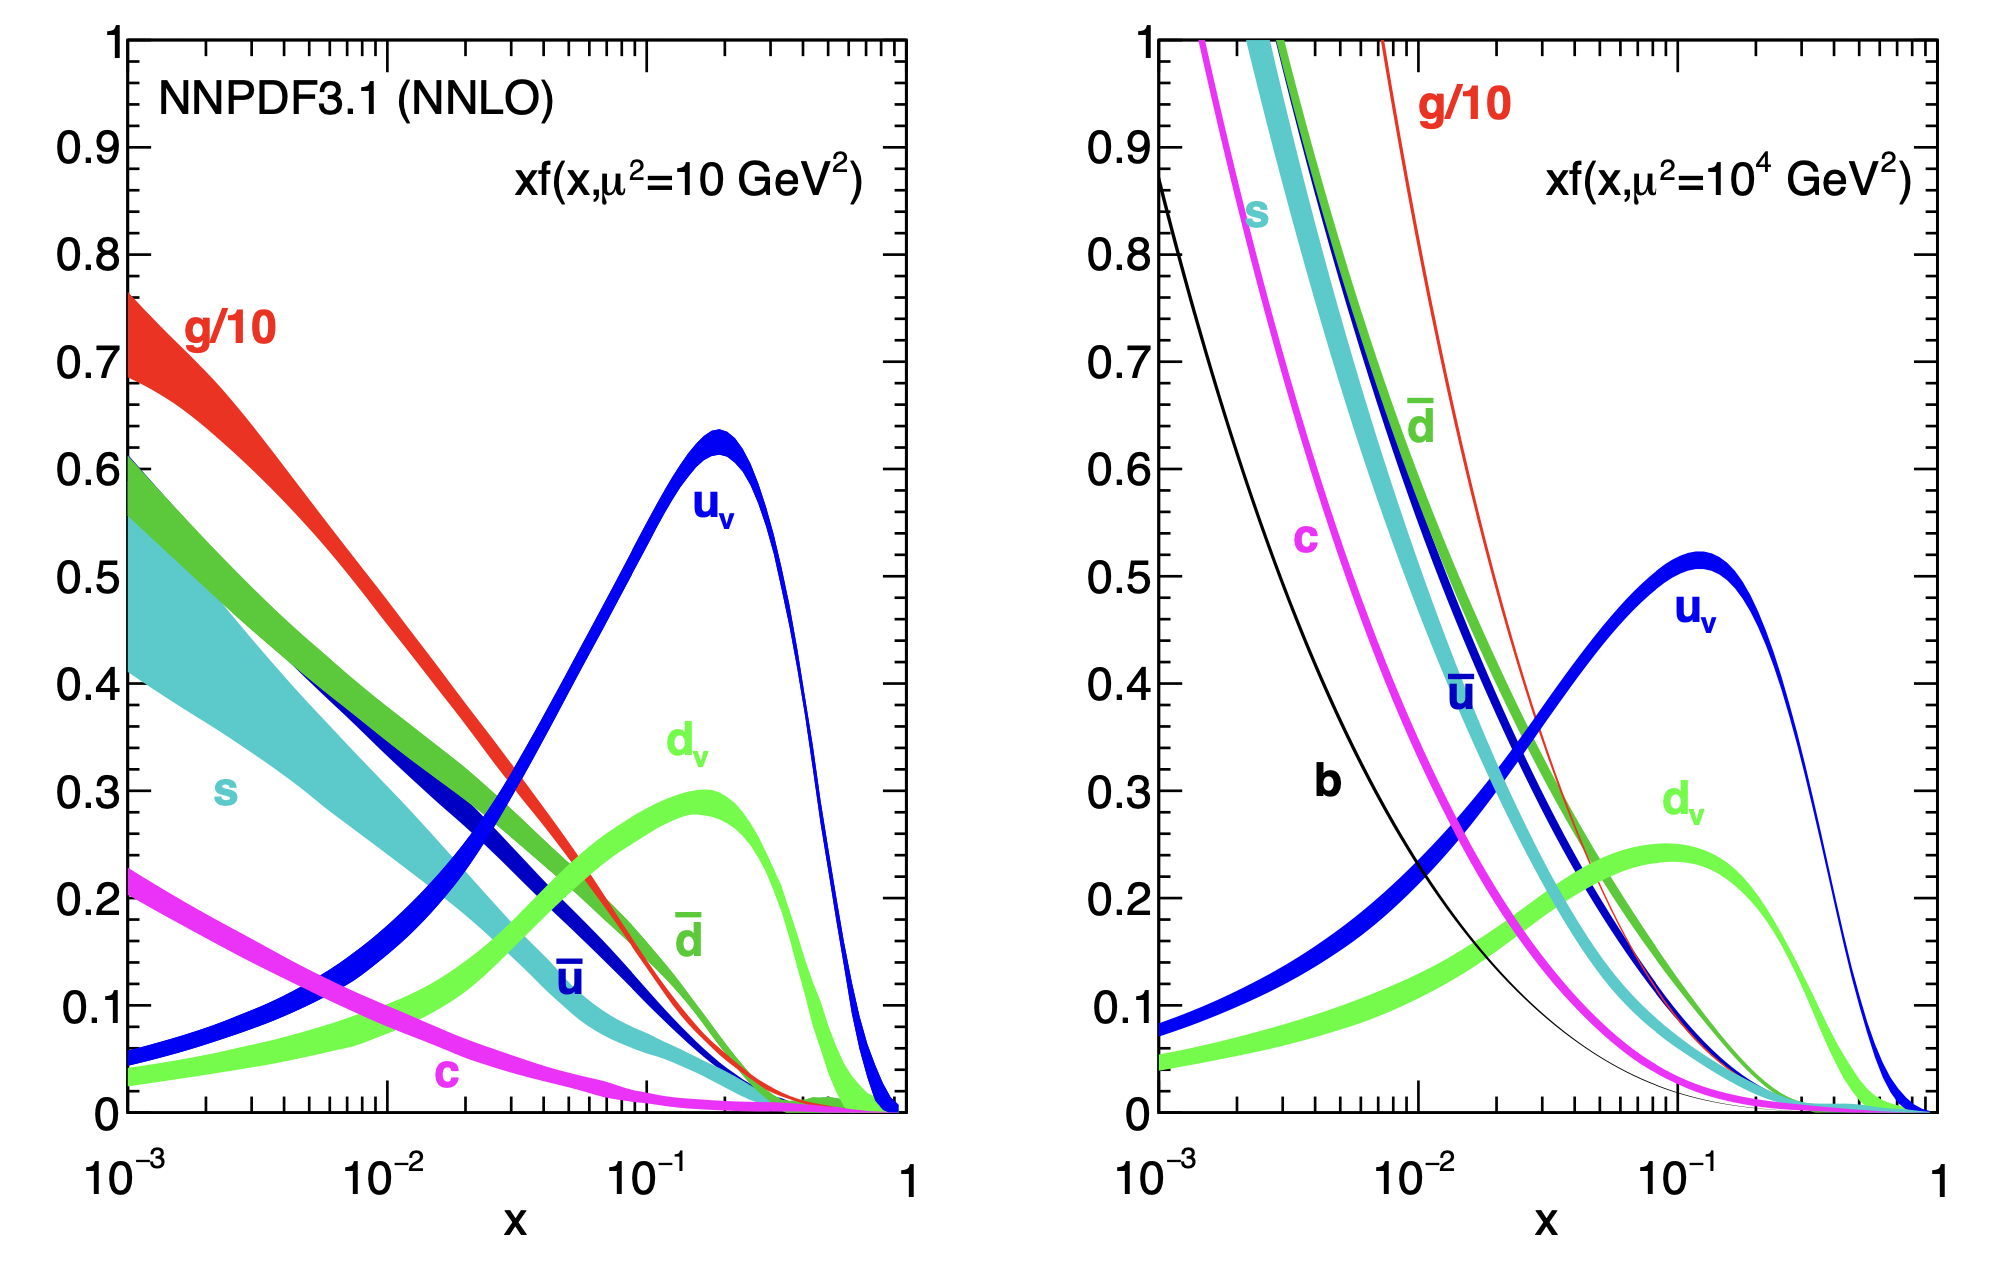
\includegraphics[width=0.95\textwidth]{protonPDFs}
\caption{Gluon and quark PDFs for the proton obtained in NNLO NNPDF3.1 analysis \cite{Ball_2017} at scale $\mu_F^2=10\,GeV^2$ (left) and $\mu_F^2=10^4\,GeV^2$ (right).}
\end{center}
\end{figure}

Gluon and sea quark distributions grow at small $x$, in particular gluon dominates at small longitudinal momentum fraction. Differently to what typically observed in elementary scattering processes, cross sections in hadron colliders increase with the energy. Indeed, we need smaller $x$ in order to produce the same mass state and the cross section grows due to the behavior of PDFs at small $x$.\\
For example, the Higgs production ($m_H\simeq 125\,GeV$) in a collision at $14\,TeV$ is dominated by gluons because, from kinematical considerations, the needed momentum fraction is $x\simeq 10^{-2}$. For this reason, the interaction between two gluons through a quark loop in order to produce the Higgs boson is the main channel for the production of this scalar particle. This process is known as the \textit{gluon gluon fusion} (ggF).\\

After the hard collision, the QCD products undergo a \textit{jet fragmentation process} due to the confinement property of strong interactions. Indeed, the signals in the detector are hadrons with high transverse momentum forming jets.\\
Firstly, soft radiations are emitted from final states of the hard scattering process. The probability of no gluon emissions above some transverse momentum is encoded in the Sudakov form factor which is used to generate the gluon distribution by Monte Carlo (MC) methods. In order to complete a real description of an event simulation, we have to include the hadronisation. Only a color-neutral collection of partons can be observed as an isolate system, then the MC event generators should implement this process. Currently, the most used implementations are based on string \cite{Andersson:1983ia} or cluster \cite{Chahal:2022rid} hadronisation models.\\
\newpage

The parton level cross section $\hat \sigma$ describes the hard scattering and is related to the fundamental interactions between elementary fields. This prediction can be calculated perturbatively because of the asymptotic freedom of QCD. The cross section is related to the squared matrix element,
\begin{align*}
	\hat \sigma(f_1 f_2 \rightarrow X)=\frac{\mathcal{S}}{2 \hat s} \int \dd \Pi_n \, \delta^{(4)}\left(\text{total momentum}\right) \left| \mathcal{A}(f_1 f_2 \rightarrow X)\right|^2,
\end{align*}
where $\mathcal{S}$ is a symmetry factor related to the identical particles in the final state and $\hat s$ is the center of mass energy for the parton process. We have to integrate over the Lorentz invariant phase space measure for the $n$ outgoing particles which are in the set $X$ and have momenta $q_i$,
$$
	\int \dd \Pi_n = \prod_i \int \frac{\dd^3 q_i}{2E_i (2\pi)^3}.
$$
The scattering amplitude $\mathcal{A}(f_1 f_2 \rightarrow X)$ is the fundamental ingredient which describes the interaction between the elementary particles. It represents a bridge between the QFT model and the phenomenology. In order to compute the amplitude, according to the traditional approach we should start from the Lagrangian, extract the Feynman rules for propagators and interaction vertices, compute all the allowed Feynman diagrams and sum together. The number of diagrams quickly increases with the number of external asymptotic states and with the number of loops. Furthermore, in squaring the amplitude, we have to compute quantum interferences between Feynman diagrams and this increases the complexity of the calculation.\\
Firstly, we can fix the polarization of the asymptotic states, namely the helicity for massless particles. The complexity is reduced because different helicity configurations do not interfere in the squared amplitude. Then we have to compute only a sum of squared helicity amplitudes,
\begin{align*}
	\left| \mathcal{A}(a+\dots \rightarrow b+\dots)\right|^2= \sum_{h_a, h_b, \dots} | \mathcal{A}(a^{h_a} +\dots \rightarrow b^{h_b} +\dots)|^2.
\end{align*}
Surprising structures of helicity amplitudes were found indeed they are simpler than the expectation from a sum of many Feynman diagrams. The complexity of helicity amplitudes depends on how much they violate the helicity conservation. The simplest structures are observed in the subset of not-vanishing helicity amplitudes which describe the processes with the maximal helicity violation, known as MHV amplitudes. In 1986, Parke and Taylor \cite{Parke:1986gb} predicted the structure of MHV amplitudes in gauge theories for an arbitrary number of gluons in terms of rational functions of kinematic invariants.\\
Moreover, the unitarity of the theory shows a connection between the discontinuity of loop amplitudes and on-shell amplitudes with lower levels of precision.
Modern techniques have been developed in order to compute one-loop and two-loop amplitudes using generalisations of the unitarity approach. One of the main reasons of the complexity of traditional computations is related to gauge redundancy. Feynman diagrams are not individually invariants differently to the result, then strong cancellations arise only when we sum together all the contributions. On-shell methods use tree-level amplitude as the building blocks for predictions of higher precision level, then they fully exploit the gauge invariance of the theory.\\

The cross section for the Higgs boson ggF production is currently known at next-to-next-to-next leading order ($\text{N}^3\text{LO}$) in QCD corrections \cite{Anastasiou_2015}. NNLO is the current level of precision of QCD corrections for the Higgs production in association with a jet \cite{Boughezal_2015}. The complexity of the computation increases with additional jets indeed for the Higgs production with two jets only NLO QCD corrections was computed \cite{an_Deurzen_2013}. These predictions are calculated in the Higgs Effective Field Theory (HEFT) in which the dominant contribution to ggF, the top-quark loop, is integrated out in the limit of infinite top mass $m_t$. This method reduces the number of loops we have to compute by one, but it is necessary a good control of the validity of this approximation. NLO predictions with the full top-mass effects are computed for the Higgs+jet production \cite{Harlander_2012, Jones_2018}. HEFT seems to works because the Higgs mass is below $2m_t$, which is the case of phenomenological interest. However, the quality of the heavy-top limit is limited by effects on Higgs' transverse momentum $p_{t,H}$: HEFT is a good approximation for $p_{t,H}<200 GeV$ as one can see in the Figure [\ref{fig:pt}]. 
\begin{figure}[H]
\begin{center}
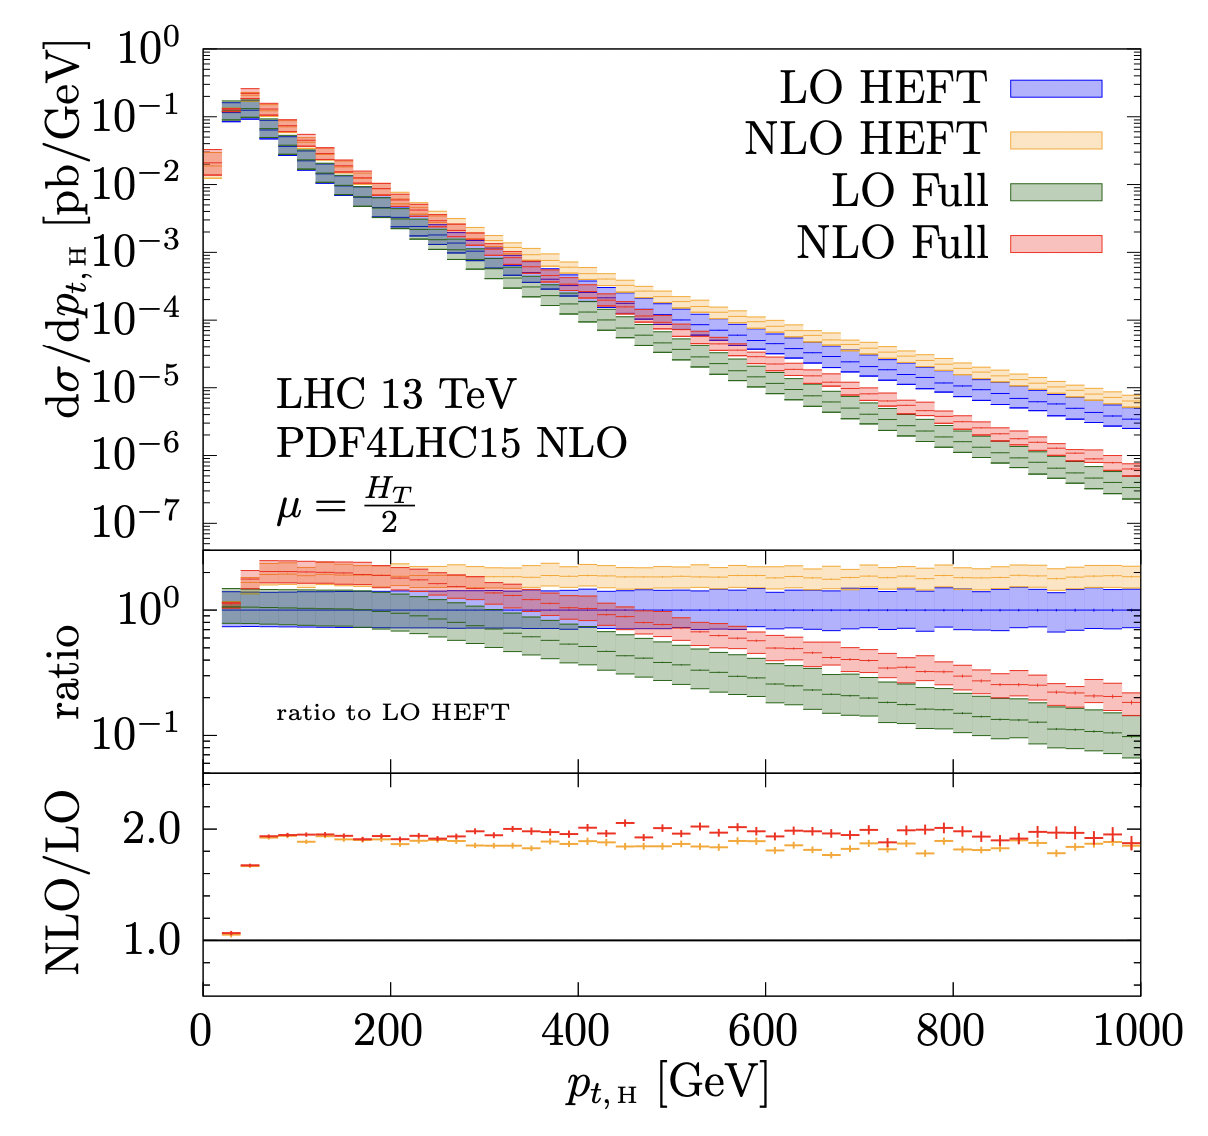
\includegraphics[width=0.6\textwidth]{Higgspt}
\caption{Higgs boson transverse momentum spectrum in QCD LO and QCD NLO for the Higgs+jet production. Comparison between the HEFT predictions and the results with the full top-mass dependence. For $p_t<200 GeV$ we observe a good agreement between the two approaches. \cite{Jones_2018}}
\label{fig:pt}
\end{center}
\end{figure}

In order to improve the level of precision for Higgs plus two jets, QCD two-loop virtual corrections represent a fundamental ingredient in NNLO computations. The desired two-loop amplitude $\mathcal{A}(gg\rightarrow Hgg)$ is not currently known in the HEFT. In an interesting version of the effective field theory, we can decompose the Higgs into two scalar fields $\phi$ and $\phi^\dagger$ whose interactions with gluons are endowed with self-dual properties. On-shell $\phi$ plus gluon amplitudes show simpler structures, in particular the MHV tree amplitude has the same form of Parke-Taylor formula.\\

In Chapter [\ref{onshellamp}], we review the spinor helicity formalism and some on-shell methods at tree and loop level. Led by the analogy between $\phi$+gluon and pure QCD MHV amplitudes, Chapter [\ref{secYM}] is devoted to the study of known one-loop and two-loop amplitudes in the all-plus sector of Yang-Mills. This represents an interesting background to learn the generalised unitarity methods in four dimensions and cuts in generic dimensions.\\
In the next chapter, we introduce the self-dual Higgs theory and we will review some useful tree and one-loop amplitudes which describe the coupling between the self-dual Higgs ($\phi$) and gluons. Also for the study of these amplitudes we implement some on-shell techniques discussed in Chapter [\ref{onshellamp}].\\
In Chapter [\ref{ch:cuts}], we compute the discontinuities of the two-loop amplitude which involves the self-dual Higgs field ($\phi$) and four gluons with positive helicity. The cut-constructible part of this amplitude represents the original result of this project.\\
In the first appendix we report the notations and the expressions for the one-loop scalar integrals.\\
In App. [\ref{appC}], we describe the computation of quadruple cuts, a generalised unitarity method applied to investigate the box contributions in the amplitude.\\
App. [\ref{phi+3g}] is devoted to the computation of the discontinuities for the amplitude at lower multiplicity considering the self-dual Higgs and only three gluons. These could be useful as a preliminary introduction for the cut computations before studying the more challenging case in Chapter [\ref{ch:cuts}]. The computation is necessary in order to check the collinear limit of the $\phi$ plus four gluon amplitude.

%\input{theory}

%% Appendix
%% ========s.

\appendix
\chapter{Scalar integrals with one or two external masses} \label{appB}
We summarise the one-loop scalar integrals with massless internal lines which we need in the computations of the project. These integrals are well-known, both analytically and numerically \cite{Ellis_2008}.
\section{Bubbles}
\begin{align*}
	I_2(s_\phi)=\left[
\begin{tikzpicture}[scale=0.8, transform shape, baseline=(current  bounding  box.center)]
     \begin{feynman}
    \vertex (x);
    \vertex[right=of x] (y);
    \path (x) ++ (180:1.5) node[vertex, label=left:$\phi$] (a);
    \path (y) ++ (-40:1.9) node[vertex] (b);
    \path (y) ++ (-20:1.9) node[vertex] (c);
    \path (y) ++ (20:1.9) node[vertex] (d);
    \path (y) ++ (40:1.9) node[vertex] (e);
    \diagram*{
        (x) --[half left, momentum=\(k\)] (y),
        (x) --[half right, rmomentum'=\(k+p_\phi\)] (y),
        (a) -- [very thick] (x),
        (y.-60) -- (b),
        (y.-30) --(c),
        (y.30) --(d),
        (y.60) -- (e),
    };
    \end{feynman}
    \end{tikzpicture}\right]=\frac{\mu^{4-d}}{i c_\Gamma}\int \frac{\dd^d k}{(2\pi)^d} \frac{1}{(k^2+i\delta)((k+p_\phi)^2+i\delta)}
\end{align*}
The parameter $\mu$ is a reference scale which guarantees the correct dimensionality, $c_\Gamma$ is defined in (\ref{defcg}) and $\delta\rightarrow 0^+$ is the standard shift of the propagators. \\
After Wick rotation, we can compute the integral using a Feynman parametrization in terms of the parameter $x_1$. After a simple substitution, we have
\begin{align*}
I_2(s_\phi)
&=\frac{\mu^{2\epsilon}}{c_\Gamma}\int_0^1 \dd x_1 \int  \frac{\dd^d k'}{(2\pi)^d} \frac{1}{[-k'^2-x_1(1-x_1)s_\phi-i\delta]}\\
&=\frac{\mu^{2\epsilon}}{c_\Gamma}\frac{\Gamma(\epsilon)}{(4\pi)^{d/2}} \int_0^1 \dd x_1 \,[-x_1(1-x_1)s_\phi-i\delta]^{-\epsilon}=\frac{\mu^{2\epsilon}}{(-s_\phi-i\delta)^\epsilon}\left[\frac{1}{\epsilon}+2\right]+\mathcal{O}(\epsilon).
\end{align*}
\section{Triangles}
In this project we need the analytic expressions for the triangles with one or two external scales and massless inner particles. Considering the one-mass triangle, 
\begin{align*}
I_3^{1m}(s_\phi)=\left[
	\begin{tikzpicture}[baseline=(current bounding box.center)]
 	 \begin{feynman}
    		\diagram [scale=0.8, small,vertical=d to b] {
      			d2 []-- [rmomentum=\(p_2\)] b --   c
        			-- [rmomentum=\(k\)] d -- b,
			d3  [particle=\(\phi\)]-- [very thick] d,
      			d4 []-- [rmomentum=\(p_1\)] c,
   		 };
  	\end{feynman}
	\end{tikzpicture}\right]=\frac{\mu^{4-d}}{i c_\Gamma}\int \frac{\dd^D k}{(2\pi)^D} \frac{1}{(k^2+i\delta)((k-p_1)^2+i\delta)((k-p_1-p_2)^2+i\delta)}
\end{align*}
The computation is similar to the previous one. After Wick rotation, we use a Feynman parametrization introducing two independent variables $x_1$ and $x_2$ and we perform the angular and radial integration in $d$-dimensions,
\begin{align*}
	I_3^{1m}(s_\phi)&=\mu^{2\epsilon}  \,\Gamma(3) \,\int_0^1 \dd x_1 \int_0^{1-x_1}\dd x_2 \int \frac{\dd^d k}{(2\pi)^d}\frac{1}{[-(1-x_1-x_2)k^2-x_1(k-p_1)^2-x_2(k-p_1-p_2)^2]^3}\\
	&=\frac{\mu^{2\epsilon}}{\epsilon^2} \frac{(-s_\phi-i\delta)^{-\epsilon}}{s_\phi}.
\end{align*}
\newpage
Similarly, we can compute the two-mass triangle,
\begin{align*}
	I_3^{2m}(s_1,s_2)=\left[
	\begin{tikzpicture}[baseline=(current bounding box.center)]
 	 \begin{feynman}
    		\diagram [scale=0.8, small, vertical=d to b] {
      			d2 [particle=\(2\)]-- [very thick] b --  c
        			-- [] d -- [] b,
			d3  [particle=\(1\)]-- [very thick] d,
      			d4 []-- [] c,
   		 };
  	\end{feynman}
	\end{tikzpicture}\right]=\frac{(-s_1-i\delta)^{-\epsilon}-(-s_2-i\delta)^{-\epsilon}}{s_1-s_2}\frac{1}{\epsilon^2}.
\end{align*}
\section{Boxes}
We need the four point scalar integrals with an off-shell leg,
\begin{align*}
	&I_4^{1m}(s_{12},s_{23};s_{45})=\left[\begin{tikzpicture}[baseline=(current bounding box.center)]
 	 \begin{feynman}
    		\diagram [small, horizontal=b to d] {
      			a -- [] b
        			-- [] c
        			-- [] d -- [rmomentum=\(k\)] a,
			d3  [particle=\(4\)]-- [] b,
			d2 [particle=\(5\)]-- [] b,
      			d1 [particle=\(1\)]-- [] a,
      			d4 [particle=\(3\)]-- [] c,
      			d -- [] s [particle=\(2\)],
   		 };
    		%\coordinate (midpoint) at ($(b)!0.75!(d)$);
   		%\draw [dashed] ($(midpoint) + (0.75, 1.35)$) -- ($(midpoint) + (-1.6, -1.3)$);
  	\end{feynman}
	\end{tikzpicture}\right]=\frac{\mu^{4-d}}{ic_\Gamma}\int \frac{\dd^d k}{(2\pi)^d} \frac{1}{D[k]D[k-p_2]D[k-P_{23}]D[k+p_1]}\\
	&=\frac{2\mu^{2\epsilon}}{s_{12}s_{23}}\left[\frac{(-s_{12})^{-\epsilon}+(-s_{23})^{-\epsilon}-(-s_{4\phi})^{-\epsilon}}{\epsilon^2}-\text{Li}_2\left(1-\frac{s_{4\phi}}{s_{12}}\right)-\text{Li}_2\left(1-\frac{s_{4\phi}}{s_{23}}\right)-\frac{1}{2}\ln^2\left(\frac{s_{12}}{s_{23}}\right)-\frac{\pi^2}{6} \right]
\end{align*}
where $D[k]=k^2+i\delta$ and the correct analytical continuation of the integral is obtained by introducing the shift $s_{ij}\rightarrow s_{ij}+i\delta$.\\
The integral can be computed with a simple change of variables for the Feynman parameters \cite{Karplus:1950zz}.\\
The structure of the divergences can be easily understood by considering the soft limits \cite{Anastasiou:2018rib}. For example, if we consider the limit in which $k\rightarrow 0$, the integral becomes
$$
	\frac{\mu^{4-d}}{i c_\Gamma} \int \frac{\dd^d k}{(2\pi)^d} \frac{1}{(k^2+i\delta)(-2k\cdot p_2-i\delta)s_{23}(+2k \cdot p_1)}=\frac{I_3^{1m}(s_{12})}{s_{23}}=\frac{\mu^{2\epsilon}}{\epsilon^2}\frac{(-s_{12}-i\delta)^{-\epsilon}}{s_{12}s_{23}}.
$$
The remainder divergent contributions are obtained by considering the soft limit of the other propagators, imposing also the collinear limit $p_4\parallel p_5$ in the case of propagators attached to the off-shell leg.\\

The other box that we have to consider has two external off-shell legs in opposite corners. This is called two-mass easy box because the computation is easier than the integral with two adjacent massive legs \cite{1994}. Indeed in this case we can perform the same substitution used to compute the one-mass box.
\begin{align*}
&I_4^{2me}(s_{1\phi},s_{4\phi};s_{\phi},s_{23})=\left[\begin{tikzpicture}[baseline=(current bounding box.center)]
 	 \begin{feynman}
    		\diagram [small,horizontal=b to d] {
      			a -- [] b
        			-- [] c
        			-- [] d -- [rmomentum=\(k\)] a,
			d3  [particle=\(3\)]-- [] b,
			d2 [particle=\(2\)]-- [] b,
      			d1 [particle=\(1\)]-- [] a,
      			d4 [particle=\(4\)]-- [] c,
      			d -- [very thick] s [particle=\(\phi\)],
   		 };
    		%\coordinate (midpoint) at ($(b)!0.75!(d)$);
   		%\draw [dashed] ($(midpoint) + (0.75, 1.35)$) -- ($(midpoint) + (-1.6, -1.3)$);
  	\end{feynman}
	\end{tikzpicture}\right]=\frac{\mu^{4-d}}{ic_\Gamma} \int \frac{\dd^d k}{(2\pi)^d} \frac{1}{D[k]D[k-p_\phi]D[k-P_{4\phi}]D[k+p_1]}\\
	&=\frac{2\mu^{2\epsilon}}{s_{1\phi}s_{4\phi}-s_{23}s_\phi}\left[\left((-s_{1\phi})^{-\epsilon}+(-s_{4\phi})^{-\epsilon}-(-s_{23})^{-\epsilon}-(-s_{\phi})^{-\epsilon}\right)\frac{1}{\epsilon^2}-\text{Li}_2\left(1-\frac{s_{\phi}}{s_{1\phi}}\right)-\text{Li}_2\left(1-\frac{s_{\phi}}{s_{4\phi}}\right)\right.\\
	&\left.\hspace{0.2cm}-\text{Li}_2\left(1-\frac{s_{23}}{s_{1\phi}}\right)-\text{Li}_2\left(1-\frac{s_{23}}{s_{4\phi}}\right)+\text{Li}_2\left(1-\frac{s_{\phi}s_{23}}{s_{1\phi}s_{4\phi}}\right)-\frac{1}{2}\ln^2\left(\frac{s_{1\phi}}{s_{4\phi}}\right)\right]
\end{align*}
The infrared structure can be obtained by considering the soft and collinear limits as observed in the one-mass box.
%%% QUADRUPLE CUTS %%%
\chapter{Quadruple cuts} \label{appC}
We explicitly compute the coefficients in front of the four-point scalar integrals in the decomposition of the two-loop amplitude. 
We will refer to these integrals indicating Mandelstam variables $s$ and $t$ and the masses, using the convention introduced in App. [\ref{appB}]. The three possible scalar boxes potentially present in our amplitude are diagrammatically described as follows. Obviously, similar contributions can be also present considering cyclic permutations of the gluons.
\begin{align}
I^{2me}_4(s_{\phi4},s_{\phi 1};m_1^2=s_{23},m_3^2=s_{\phi})&=
\begin{tikzpicture}[baseline=(current bounding box.center)]
 	 \begin{feynman}
    		\diagram [horizontal=b to d] {
      			a -- [] b
        			-- [] c
        			-- [] d -- [] a,
			d3  [particle=\(3\)]-- [] b,
			d2 [particle=\(2\)]-- [] b,
      			d1 [particle=\(1\)]-- [] a,
      			d4 [particle=\(4\)]-- [] c,
      			d -- [very thick] s [particle=\(\phi\)],
   		 };
    		%\coordinate (midpoint) at ($(b)!0.75!(d)$);
   		%\draw [dashed] ($(midpoint) + (0.75, 1.35)$) -- ($(midpoint) + (-1.6, -1.3)$);
  	\end{feynman}
	\end{tikzpicture}	\label{sbox:2me}\\
	I^{2mh}_4(s_{14},s_{\phi 1};m_1^2=s_{23},m_2^2=s_{\phi})&=
\begin{tikzpicture}[baseline=(current bounding box.center)]
 	 \begin{feynman}
    		\diagram [horizontal=b to d] {
      			a -- [] b
        			-- [] c
        			-- [] d -- [] a,
			d3  [particle=\(3\)]-- [] b,
			d2 [particle=\(2\)]-- [] b,
      			d1 [particle=\(\phi\)]-- [very thick] a,
      			d4 [particle=\(4\)]-- [] c,
      			d -- [] s [particle=\(1\)],
   		 };
    		%\coordinate (midpoint) at ($(b)!0.75!(d)$);
   		%\draw [dashed] ($(midpoint) + (0.75, 1.35)$) -- ($(midpoint) + (-1.6, -1.3)$);
  	\end{feynman}
	\end{tikzpicture}	 \label{sbox:2mh}\\
	I^{1m}_4(s_{14},s_{12};m^2=s_{3\phi})&=
\begin{tikzpicture}[baseline=(current bounding box.center)]
 	 \begin{feynman}
    		\diagram [horizontal=b to d] {
      			a -- [] b
        			-- [] c
        			-- [] d -- [] a,
			d3  [particle=\(3\)]-- [] b,
			d2 [particle=\(\phi\)]-- [very thick] b,
      			d1 [particle=\(2\)]-- [] a,
      			d4 [particle=\(4\)]-- [] c,
      			d -- [] s [particle=\(1\)],
   		 };
    		%\coordinate (midpoint) at ($(b)!0.75!(d)$);
   		%\draw [dashed] ($(midpoint) + (0.75, 1.35)$) -- ($(midpoint) + (-1.6, -1.3)$);
  	\end{feynman}
	\end{tikzpicture}	 \label{sbox:1m}
\end{align}
We have to study three different topologies in order to extract the coefficient in front of the two-mass easy box (\ref{sbox:2me}), the two-mass hard box (\ref{sbox:2mh}) and the four-point integral with an off-shell leg ( \ref{sbox:1m}).
\section{First sector with a one-loop $\phi$+gluon sub-amplitude}
We have to compute the quadruple cuts for the three possible four-point configurations imposing the four on-shell constraints for the inner gluons and studying all the possible helicity organizations of the sub-amplitudes. We start considering the first sector in which the $\phi$+gluon sub-amplitude is considered at one-loop level.
\subsubsection{Easy two-mass box}
We start considering the following quadruple cut in the two-mass easy configuration.
\begin{center}
\tikzfeynmanset{ myblob/.style={ shape=circle, typeset=$\bigcirc$,
draw=black, } }
\feynmandiagram [] {
a [particle=\(\phi\)] -- [scalar] t1 [myblob] -- [gluon, momentum=\(\ell_2\)] t2 [blob] -- [gluon,momentum=\(\ell_3\)] t3  [blob] -- [gluon, momentum=\(\ell_4\)] t4 [blob] -- [gluon, momentum=\(\ell_1\)] t1, t2 -- [gluon] p1 [particle=\(1^+\)],
t3 -- [gluon] p2 [particle=\(2^+\)], t3 -- [gluon] p3 [particle=\(3^+\)], t4 -- [gluon] p4 [particle=\(4^+\)],
};
\end{center}
The loop momenta are
$$
	\left\{\ell_1,\ \ell_2,\ \ell_3,\ \ell_4\right\}=\left\{\ell_1,\ \ell_1-p_\phi,\ \ell_1-p_\phi-p_1,\ \ell_1+p_4\right\}.
$$
We impose the on-shell conditions $\ell_i^2=0$ and we obtain
\begin{align*}
	&\left\{\ell_1^2=0,\ \ell_1\cdot p_\phi=\frac{m_H^2}{2},\ \ell_1\cdot p_4=0,\ \ell_1\cdot p_{\phi1}=\frac{s_{\phi1}}{2}\right\},\\
	&\left\{\ell_1^2=0,\ \ell_1\cdot p_\phi=\frac{m_H^2}{2},\ \ell_1\cdot p_4=0,\ \ell_1\cdot p_{1}=\frac{s_{\phi1}-m_H^2}{2}\right\}. \numthis \label{eq:4cphicond}
\end{align*}
We consider the following decomposition of the loop momentum,
$$
	\ell_1^\mu=a_1 p_1^\mu+ a_4 p_4^\mu +d_1 \frac{\langle 1\sigma^\mu 4]}{2}+d_4\frac{\langle 4\sigma^\mu 1]}{2}
$$
where $a_1, a_4, d_1, d_4$ are coefficients we determine using on-shell conditions (\ref{eq:4cphicond}).\\We start considering the constraints
\begin{align*}
	&\ell_1\cdot p_4=a_1 p_1 \cdot p_4=0 \Rightarrow a_1=0 \\
	&\ell_1\cdot p_1=a_4 p_4 \cdot p_1=\frac{s_{\phi1}-m_H^2}{2} \Rightarrow a_4=\frac{s_{\phi1}-m_H^2}{s_{41}}.
\end{align*}
Now we want to impose the condition $\ell_1^2=0$,
\begin{align*}
	&a_1 \ell_1 \cdot p_1+a_4 \ell_1\cdot p_4+d_1 \frac{\langle 1\ell_1 4]}{2}+d_4\frac{\langle 4 \ell_1 1]}{2}=0\\
	&2a_1 a_4(\ell_1\cdot p_4)-2d_1d_4 p_{4}\cdot p_1=0\\
	&d_1d_4=a_1a_2=0 \Rightarrow d_1=0 \text{ or } d_4=0.
\end{align*}
We have two possible solutions and the last constraint on the product $\ell_1\cdot p_\phi$ fixes the remainder non-vanishing coefficient. In conclusion we have the solutions,
\begin{align*}
	&\ell_1^{(1)}=a_4p_4^\mu +d_1\frac{\langle1\sigma^\mu4]}{2} \text{ with } \begin{cases}
		a_4=\frac{s_{\phi1}-s_\phi}{s_{41}}\\d_1=\frac{1}{\langle 1\phi 4]}\left(s_\phi-\frac{(s_{\phi1}-s_\phi)(s_{\phi4}-s_\phi)}{s_{41}}\right)
	\end{cases},\\
	&\ell_1^{(2)}=a_4p_4^\mu +d_4\frac{\langle4\sigma^\mu1]}{2} \text{ with } \begin{cases}
		a_4=\frac{s_{\phi1}-s_\phi}{s_{41}}\\d_4=\frac{1}{\langle 4\phi 1]}\left(s_\phi-\frac{(s_{\phi1}-s_\phi)(s_{\phi4}-s_\phi)}{s_{41}}\right)
	\end{cases}.	\numthis \label{solveasyquadruplekin}
\end{align*}
Using the property $2\ell_1^\mu=\langle \ell_1|\sigma^\mu|\ell_1]$, we can write the spinors of the solutions in the following way.
\begin{align}
	&\begin{cases}
		|\ell_1^{(1)}\rangle=a_4|4\rangle+d_1|1\rangle\\
		|\ell_1^{(1)}]=|4]
	\end{cases}\\
	&\begin{cases}
		|\ell_1^{(2)}\rangle=|4\rangle\\
		|\ell_1^{(2)}]=a_4|4]+d_4|1]
	\end{cases}	\label{eq:spin2}
\end{align}
After the kinematic considerations, we can study the quadruple cut of the two-loop amplitude which corresponds to the sum over the allowed helicity configurations of the products with trees and one-loop factors. There is only one allowed helicity configuration which has a non-vanishing tree-level four gluon amplitude. 
%In addition to the two positive external gluons, we need the negative helicity for the two internal particles connected to the concerned sub-amplitude represented in the following figure with a violet vertex. This fact completely fixes the helicity of all the gluons.
\definecolor{asparagus}{rgb}{0.53, 0.66, 0.42}
\begin{center}
\tikzfeynmanset{ myblob/.style={ shape=circle, typeset=$\bigcirc$,
draw=black, } }
\feynmandiagram [] {
a [particle=\(\phi\)] -- [scalar] t1 [myblob, label={[orange]180:\(+\)}, label={[asparagus]0:\(+\)}] -- [gluon, asparagus] t2 [blob, label={[asparagus]90:\(-\)}, label={[blue]-90:\(+\)}] -- [gluon, blue] t3  [blob, violet, label={[blue]0:\(-\)}, label={[red]180:\(-\)}] -- [gluon, red] t4 [blob, label={[red]-90:\(+\)}, label={[orange]90:\(-\)}] -- [gluon, orange] t1, t2 -- [gluon] p1 [particle=\(1^+\)],
t3 -- [gluon] p2 [particle=\(2^+\)], t3 -- [gluon] p3 [particle=\(3^+\)], t4 -- [gluon] p4 [particle=\(4^+\)],
};
\end{center}
We only have to compute the following contribution,
\begin{align*}
	c_{2me}(\ell_1)\coloneqq&A^{tree}(2^+,3^+,\ell_4^-,(-\ell_3)^-) A^{tree}(4^+,(-\ell_4)^+, \ell_1^-) \\&A^{1L}(\phi;(-\ell_1)^+\ell_2^+)A^{tree}(1^+,(-\ell_2)^-\ell_3^+)\\
	=&\frac{\langle \ell_4 \ell_3\rangle^3}{\langle 23 \rangle \langle 3\ell_4 \rangle \langle \ell_3 2\rangle}\frac{[\ell_4 4]^3}{[4\ell_1][\ell_1\ell_4]}\frac{-2s_\phi^2}{\langle \ell_1 \ell_2\rangle\langle \ell_2\ell_1\rangle}\frac{[1\ell_3]^3}{[\ell_3\ell_2][\ell_2 1]}\\
	=&\frac{2s_\phi^2}{\langle 23\rangle}\frac{[4\ell_4\ell_3 1]^3}{[4\ell_1\ell_2 1]\langle 3\ell_4\ell_1\ell_2\ell_3 2\rangle}=\frac{-2 s_\phi^2}{\langle 12 \rangle \langle 23 \rangle\langle 34 \rangle\langle 41 \rangle} \langle 14\ell_1 \phi 1]
\end{align*}
We immediately observe that $c_{2me}(\ell_1^{(1)})=0$: this is due to the relation $|\ell_1^{(1)}]=|4]$.\\Using the second solution and in particular the spinors (\ref{eq:spin2}), we can compute the only non-trivial contribution,
\begin{align*}
	c_{2me}(\ell_1^{(2)})&=A^{1L}(\phi;1^+,2^+,3^+,4^+) \langle 14\ell_1^{(2)}]\langle \ell_1^{(2)} \phi 1]\\
	&=A^{1L}(\phi;1^+,2^+,3^+,4^+) \left(s_{14}s_\phi-(s_{\phi 1}-s_\phi)(s_{\phi 4}-s_\phi)\right).
\end{align*}

Now we are able to extract the coefficient in front of the box integral with massless inner lines and two external masses $s_\phi$ and $s_{23}$ at diagonally opposite corners.
To connect the desired coefficients with the generalized unitarity cuts, it is useful to introduce the following vector, orthogonal to three given Lorentz vectors $p_a,p_b,p_c$,
$$
	\omega^\mu(p_a,p_b,p_c)=N_\omega\left(\langle a\sigma^\mu b]\langle b c a]-\langle b \sigma^\mu a]\langle acb]\right),
$$
where $N_\omega$ represents a normalization constant.\\
From the Section [\ref{sec:ISPs}], we know that a general decomposition of a scalar box integral is
$$
	\int \frac{\dd^d k}{(2\pi)^d}\frac{\Delta(k)}{D_0D_1D_2D_3},\ \  \begin{cases}
		\Delta(k)=d_1+d_2 (k\cdot n )\\
		{D_i}=\text{ propagators}
	\end{cases}
$$
The contribution proportional to $(k\cdot n)$ is a spurious term that vanishes after the integration. If we fix the generic direction $n$ in order to be equal to the vector $\omega^\mu(p_1,p_4,p_\phi)$, we have
\begin{align*}
	\mathcal{D}_{2me}(\ell_1^{(1)})&=d_1^{(2me)}+d_2^{(2me)}(\ell_1^{(1)}\cdot \omega)\equiv c_{2me}(\ell_1^{(1)})\\
	\mathcal{D}_{2me}(\ell_1^{(2)})&=d_1^{(2me)}+d_2^{(2me)}(\ell_1^{(2)}\cdot \omega)=d_1^{(2me)}-d_2^{(2me)}(\ell_1^{(1)}\cdot \omega)\equiv c_{2me}(\ell_1^{(2)}).
\end{align*}
Therefore the coefficient in front of the integrated object $I_4^{2me}(s_{\phi4},s_{1\phi};s_{23},s_{\phi})$ is
\begin{align}
	d_1^{(2me)}&=\frac{1}{2}\left(c_{2me}(\ell_1^{(1)})+c_{2me}(\ell_1^{(2)})\right)	\label{eq:coeffquad}\\
	&=\frac{1}{2}A^{1L}(\phi;1^+,2^+,3^+,4^+) \left(s_{14}s_\phi-(s_{\phi 1}-s_\phi)(s_{\phi 4}-s_\phi)\right).	\label{eq:2meboxcoef}
\end{align}
\subsubsection{Hard two-mass box}
An other possible configuration, that we can study through quadruple cuts, includes two external masses at adjacent corners.
\begin{center}
\tikzfeynmanset{ myblob/.style={ shape=circle, typeset=$\bigcirc$,
draw=black, } }
\feynmandiagram [horizontal'=p4 to t2] {
a [particle=\(\phi\)] -- [scalar] t1 [myblob] -- [gluon, momentum=\(\ell_2\)] t2 [blob] -- [gluon, momentum=\(\ell_3\)] t3  [blob] -- [gluon, momentum=\(\ell_4\)] t4 [blob] -- [gluon, momentum=\(\ell_1\)] t1, t2 -- [gluon] p1 [particle=\(2^+\)],
t2 -- [gluon] p2 [particle=\(1^+\)], t3 -- [gluon] p3 [particle=\(3^+\)], t4 -- [gluon] p4 [particle=\(4^+\)],
};
\end{center}
In this case, the loop momenta are
$$
	\left\{\ell_1,\ \ell_2,\ \ell_3,\ \ell_4\right\}=\left\{\ell_1,\ \ell_1-p_\phi,\ \ell_1+p_4+p_3,\ \ell_1+p_4\right\}.
$$
We choose the following parametrization of the loop momentum $\ell_1$,
$$
	\ell_1^\mu=a_3 p_3^\mu+a_4 p_4^\mu +d_3 \frac{\langle 3 \sigma^\mu 4]}{2}+d_4 \frac{\langle 4 \sigma^\mu 3]}{2}.
$$
The quadruple cut requires the on-shell conditions $\ell_i^2=0$ and, using these constraints, we find the solutions,
\begin{align}
	&\ell_1^{(1)}=-p_4^\mu +d_3\frac{\langle3\sigma^\mu4]}{2} \ \ \text{with} \ \ d_3=\frac{s_{4\phi}}{\langle 3\phi4]}, \label{eq:sol1h}\\
	&\ell_1^{(2)}=-p_4^\mu +d_4\frac{\langle4\sigma^\mu3]}{2} \ \ \text{with} \ \ d_4=\frac{s_{4\phi}}{\langle4\phi 3]}.
\end{align}
Cutting the two-loop amplitude, we have only the following contribution due to the fact that the tree-level four gluon amplitude with two external positive gluons requires the negative helicity for the other two particles.
\begin{align*}
	c_{2mh}(\ell_1)\coloneqq&A^{tree}(3^+,(-\ell_3)^+,\ell_4^-) A^{tree}(4^+,(-\ell_4)^+, \ell_1^-) \\&A^{1L}(\phi;(-\ell_1)^+\ell_2^+)A^{tree}(1^+,2^+,\ell_3^-,(-\ell_2)^-)\\
	=&\frac{[3\ell_3]^3}{[\ell_3\ell_4][\ell_4 3]]}\frac{[4\ell_4]^3}{[\ell_4\ell_1][\ell_1 4]}\frac{-2s_\phi^2}{\langle \ell_1\ell_2\rangle\langle\ell_2\ell_1\rangle}\frac{\langle \ell_3\ell_2\rangle^3}{\langle 12 \rangle\langle 2\ell_3 \rangle \langle \ell_2 1 \rangle}
\end{align*}
Remembering that $\ell_4=\ell_1+p_4$, from the solution (\ref{eq:sol1h}) we find the expressions for the spinors associated to the gluon with momenta $\ell_1^{(1)}$ and $\ell_4^{(1)}$:
\begin{align}
	\begin{cases}
		|\ell_1^{(1)}\rangle=-|4\rangle+d_3|3\rangle \\
		|\ell_1^{(1)}]=|4]
	\end{cases} \ \Rightarrow 
	\begin{cases}
		|\ell_4^{(1)}\rangle=d_3|3\rangle \\
		|\ell_4^{(1)}]=|4]
	\end{cases}
	\label{quadA}.
\end{align}
The relation $|\ell_4^{(1)}]=|4]$ shows us that the anti-MHV amplitude $A^{tree}(4^+,(-\ell_4)^+, \ell_1^-)$ vanishes if we consider the first solution, therefore
$
	c_{2mh}(\ell_1^{(1)})=0
$.\\
Similar considerations hold for the second solution, in fact the spinors associated to the momenta $\ell_1^{(2)}$ and $\ell_3^{(2)}=\ell_1^{(2)}+p_3+p_4$ are
\begin{align}
	\begin{cases}
		|\ell_1^{(2)}\rangle=|4\rangle \\
		|\ell_1^{(2)}]=-|4]+d_4|3]
	\end{cases} \ \Rightarrow 
	\begin{cases}
		|\ell_3^{(2)}\rangle=|4\rangle+\frac{1}{d_4}|3\rangle \\
		|\ell_3^{(2)}]=d_4|4]
	\end{cases}.
	\label{quadB}
\end{align}
The last relation implies that $$A^{tree}(3^+,(-\ell_3)^+,\ell_4^-)=0\  \Rightarrow \ c_{2mh}(\ell_3^{(2)})=0.$$
In conclusion the coefficient investigated using this quadruple cut vanishes and therefore in this sector we observe the absence of a contribution proportional to the integral $I_{4}^{2mh}(s_{34},s_{4\phi};s_{12},s_\phi)$.
\subsubsection{One-mass box}
The last configuration we have to consider is the following one-mass box.
\begin{center}
\tikzfeynmanset{ myblob/.style={ shape=circle, typeset=$\bigcirc$,
draw=black, } }
\feynmandiagram [vertical=t1 to p3] {
a [particle=\(1^+\)] -- [gluon] t1 [myblob] -- [gluon, momentum'=\(\ell_2\)] t2 [blob] -- [gluon,momentum'=\(\ell_3\)] t3  [blob] -- [gluon, momentum'=\(\ell_4\)] t4 [blob] -- [gluon, momentum'=\(\ell_1\)] t1, t1 -- [scalar] p1 [particle=\(\phi\)], t3 -- [gluon] p3 [particle=\(3^+\)], t2 -- [gluon] p2 [particle=\(2^+\)], t4 -- [gluon] p4 [particle=\(4^+\)],
};
\end{center}
If we express $\ell_1$ in the decomposition
$$
	\ell_1^\mu=a_3 p_3^\mu +a_4 p_4^\mu +d_3\frac{\langle 3 \sigma^\mu 4]}{2}+d_4 \frac{\langle 4 \sigma^\mu 3]}{2},
$$
we can determine the coefficients to satisfy the on-shell constraints,
\begin{align*}
	&\left\{\ell_1,\ \ell_2,\ \ell_3,\ \ell_4\right\}=\left\{\ell_1,\ \ell_1-p_\phi-p_1,\ \ell_1+p_3+p_4,\ \ell_1+p_4\right\}=\{0,0,0,0\}.
\end{align*}
We find two solutions,
\begin{align}
	&\ell_1^{(1)}=-p_4^\mu +d_3\frac{\langle3\sigma^\mu4]}{2} \ \ \text{with} \ \ d_3=\frac{s_{\phi1}-s_{24}-s_{34}}{\langle 324]}, \\
	&\ell_1^{(2)}=-p_4^\mu +d_4\frac{\langle4\sigma^\mu3]}{2} \ \ \text{with} \ \ d_4=\frac{s_{\phi1}-s_{24}-s_{34}}{\langle423]}.
\end{align}
We have to study the possible helicity configurations: the non-trivial possibilities are represented by the following diagrams.
\begin{center}
\tikzfeynmanset{ myblob/.style={ shape=circle, typeset=$\bigcirc$,
draw=black} }
\scalebox{0.88}{
\begin{tikzpicture}
  \begin{feynman}
    \diagram [vertical=t1 to p3] {
a [particle=\(1^+\), label=-90:\(\hspace{-2.3cm}(A)\)] -- [gluon] t1 [myblob, label={[purple]0:\(-\)}, label={[text=orange]180:\(+\)}] -- [gluon, orange] t2 [blob, magenta, label={[orange]90:\(-\)}, label={[teal]-90:\(+\)}] -- [gluon, teal] t3  [blob, magenta, label={[teal]180:\(-\)}, label={[violet]0:\(+\)}] -- [gluon, violet] t4 [blob, magenta, label={[violet]-90:\(-\)}, label={[purple]90:\(+\)}] -- [gluon,purple] t1, t1 -- [scalar] p1 [particle=\(\phi\)], t3 -- [gluon] p3 [particle=\(3^+\)], t2 -- [gluon] p2 [particle=\(2^+\)], t4 -- [gluon] p4 [particle=\(4^+\)],
};
\end{feynman}
\end{tikzpicture}
}
\scalebox{0.88}{
\feynmandiagram [vertical=t1 to p3] {
a [particle=\(1^+\), label=-90:\(\hspace{-2.3cm}(B)\)] -- [gluon] t1 [myblob, label={[purple]0:\(+\)}, label={[text=orange]180:\(-\)}] -- [gluon, orange] t2 [blob, magenta, label={[orange]90:\(+\)}, label={[teal]-90:\(-\)}] -- [gluon, teal] t3  [blob, magenta, label={[teal]180:\(+\)}, label={[violet]0:\(-\)}] -- [gluon, violet] t4 [blob, magenta, label={[violet]-90:\(+\)}, label={[purple]90:\(-\)}] -- [gluon,purple] t1, t1 -- [scalar] p1 [particle=\(\phi\)], t3 -- [gluon] p3 [particle=\(3^+\)], t2 -- [gluon] p2 [particle=\(2^+\)], t4 -- [gluon] p4 [particle=\(4^+\)],
};
}
\scalebox{0.88}{
\feynmandiagram [vertical=t1 to p3] {
a [particle=\(1^+\), label=-90:\(\hspace{-2.3cm}(C)\)] -- [gluon] t1 [myblob, label={[purple]0:\(+\)}, label={[text=orange]180:\(+\)}] -- [gluon, orange] t2 [blob, magenta, label={[orange]90:\(-\)}, label={[teal]-90:\(+\)}] -- [gluon, teal] t3  [blob, magenta, label={[teal]180:\(-\)}, label={[violet]0:\(+\)}] -- [gluon, violet] t4 [blob, cyan, label={[violet]-90:\(-\)}, label={[purple]90:\(-\)}] -- [gluon,purple] t1, t1 -- [scalar] p1 [particle=\(\phi\)], t3 -- [gluon] p3 [particle=\(3^+\)], t2 -- [gluon] p2 [particle=\(2^+\)], t4 -- [gluon] p4 [particle=\(4^+\)],
};
}
\\
\scalebox{0.88}{
\feynmandiagram [vertical=t1 to p3] {
a [particle=\(1^+\), label=-90:\(\hspace{-2.3cm}(D)\)] -- [gluon] t1 [myblob, label={[purple]0:\(+\)}, label={[text=orange]180:\(+\)}] -- [gluon, orange] t2 [blob, cyan, label={[orange]90:\(-\)}, label={[teal]-90:\(-\)}] -- [gluon, teal] t3  [blob, magenta, label={[teal]180:\(+\)}, label={[violet]0:\(-\)}] -- [gluon, violet] t4 [blob, magenta, label={[violet]-90:\(+\)}, label={[purple]90:\(-\)}] -- [gluon,purple] t1, t1 -- [scalar] p1 [particle=\(\phi\)], t3 -- [gluon] p3 [particle=\(3^+\)], t2 -- [gluon] p2 [particle=\(2^+\)], t4 -- [gluon] p4 [particle=\(4^+\)],
};
}
\scalebox{0.88}{
\feynmandiagram [vertical=t1 to p3] {
a [particle=\(1^+\), label=-90:\(\hspace{-2.3cm}(E)\)] -- [gluon] t1 [myblob, label={[purple]0:\(+\)}, label={[text=orange]180:\(+\)}] -- [gluon, orange] t2 [blob, magenta, label={[orange]90:\(-\)}, label={[teal]-90:\(+\)}] -- [gluon, teal] t3  [blob, cyan, label={[teal]180:\(-\)}, label={[violet]0:\(-\)}] -- [gluon, violet] t4 [blob, magenta, label={[violet]-90:\(+\)}, label={[purple]90:\(-\)}] -- [gluon,purple] t1, t1 -- [scalar] p1 [particle=\(\phi\)], t3 -- [gluon] p3 [particle=\(3^+\)], t2 -- [gluon] p2 [particle=\(2^+\)], t4 -- [gluon] p4 [particle=\(4^+\)],
};
}
\hspace{2.1cm}
\feynmandiagram[small, vertical=s to t]{
	u -- [white] u2 -- [white] u3 -- [white]  s [blob, magenta, label={0:\(=\text{ anti-MHV}\)}] -- [white]  t [blob, cyan, label={0:\(=\text{ MHV}\)}],
};
\end{center}
If we consider the first solution in which the spinors are
\begin{align*}
	\begin{cases}
	|\ell_1^{(1)}]\propto|\ell_4^{(1)}]\propto|4]\\
	|\ell_4^{(1)}\rangle\propto|\ell_3^{(1)}\rangle\propto|3\rangle
	\end{cases},
\end{align*}
we immediately observe that:
\begin{enumerate}
\item the diagrams $(A)$ and $(C)$ vanish, indeed
	$$A^{tree}(3^+,(-\ell_3)^-,\ell_4^+) = 
	\feynmandiagram[inline=(v.base),small,vertical=v to a]{
		a [particle=\(3^+\)] -- [gluon] v [blob, magenta, label={180:\(-\)}, label={0:\(+\)}] -- [gluon, rmomentum'=\(\ell_3\)] b,
		v -- [gluon, momentum=\(\ell_4\)] c,
	};
	\propto [3\ell_4^{(1)}]^3=0;$$
\item the diagrams $(B)$ and $(D)$ are zero due to the relation 
	$$A^{tree}(4^+,(-\ell_4)^+,\ell_1^-) = 
	\feynmandiagram[inline=(v.base),small,horizontal=v to a]{
		a [particle=\(4^+\)] -- [gluon] v [blob, magenta, label={-90:\(+\)}, label={90:\(-\)}] -- [gluon, rmomentum'=\(\ell_4\)] b,
		v -- [gluon, momentum=\(\ell_1\)] c,
	};
	\propto [ \ell_4^{(1)} 4 ]^3=0;$$
\item the diagram $(E)$ vanishes because of the presence of the following factor:
	$$A^{tree}(3^+,(-\ell_3)^-,\ell_4^-) = 
	\feynmandiagram[inline=(v.base),small,vertical=v to a]{
		a [particle=\(3^+\)] -- [gluon] v [blob, cyan, label={180:\(-\)}, label={0:\(-\)}] -- [gluon, rmomentum'=\(\ell_3\)] b,
		v -- [gluon, momentum=\(\ell_4\)] c,
	};
	\propto \langle \ell_3^{(1)}\ell_4^{(1)}\rangle^3=0.$$
\end{enumerate}
Therefore we have no contributions considering the first solution $\ell_1^{(1)}$.\\
For the second solution, we observe that $|\ell_4^{(2)}]\propto|\ell_3^{(2)}]\propto|3]$.
These relations simplify the calculation because four diagrams are zero due to the following vanishing sub-amplitudes.
\begin{align*}
	&\feynmandiagram[inline=(v.base),small,vertical=v to a]{
		a [particle=\(3^+\)] -- [gluon] v [blob, magenta, label={180:\(-\)}, label={0:\(+\)}] -- [gluon, rmomentum'=\(\ell_3\)] b,
		v -- [gluon, momentum=\(\ell_4\)] c,
	};
	\propto [3\ell_4^{(2)}]^3=0 \Rightarrow \begin{cases}
	(A)=0\\ (C)=0
	\end{cases}\\
	&\feynmandiagram[inline=(v.base),small,vertical=v to a]{
		a [particle=\(3^+\)] -- [gluon] v [blob, magenta, label={180:\(+\)}, label={0:\(-\)}] -- [gluon, rmomentum'=\(\ell_3\)] b,
		v -- [gluon, momentum=\(\ell_4\)] c,
	};
	\propto [3\ell_3^{(2)}]^3=0 \Rightarrow \begin{cases}(B)=0\\ (D)=0 \end{cases}\\
\end{align*}
The only non-trivial contribution is represented by the diagram with the gluon $3^+$ associated to a MHV vertex $(E)$,
\begin{align*}
	c_{1m}(\ell_1)&=A^{tree}(3^+,\ell_4^-,(-\ell_3)^-)A^{tree}((-\ell_4)^+,4^+,\ell_1^-)A^{1L}(\phi;1^+,(-\ell_1)^+,\ell_2^+)A^{tree}((-\ell_2)^-,2^+,\ell_3^+)\\
	&=\frac{\langle \ell_4\ell_3\rangle^3}{\langle \ell_3 3 \rangle\langle 3 \ell_4 \rangle}\frac{[\ell_4 4]^3}{[4\ell_1][\ell_1\ell_4]}\frac{-2s_\phi^2}{\langle \ell_2 \ell_1 \rangle \langle \ell_1 1 \rangle \langle 1 \ell_2 \rangle}\frac{[2\ell_3]^3}{[\ell_3\ell_2][\ell_2 2]}.
\end{align*}
Using the momentum conservation laws together with some simple spinor algebra, we obtain
$$
	c_{1m}(\ell_1)=\frac{-2m_H^4}{\langle 21\rangle}\frac{[34]\langle \ell_4\ell_3\rangle^2 [\ell_4 4][2 \ell_3]}{\langle 3 \ell_4 \rangle \langle 1 \ell_4 \rangle [\ell_1\ell_4]\langle \ell_1 \ell_3 \rangle}.
$$
Now we explicitly use the spinors of the second solution $\ell_1^{(2)}$ and we find
\begin{align*}
	c_{1m}(\ell_1^{(2)})=\frac{-2s_\phi^2}{\langle 21 \rangle}\frac{[34][23]}{\langle 41 \rangle}=-s_{34}s_{23}A^{1L}(\phi;1^+2^+3^+4^+).
\end{align*}
As shown in the easy two-mass case (\ref{eq:coeffquad}), the desired coefficient is the arithmetic average of the results from the two solutions of the loop momentum:
\begin{equation}
	d_1^{1m}=\frac{1}{2}\left(c_{1m}(\ell_1^{(1)})+c_{1m}(\ell_1^{(2)})\right)=-\frac{1}{2}s_{34}s_{23}A^{1L}(\phi;1^+,2^+,3^+,4^+)	\label{eq:d11m}
\end{equation}
\subsubsection{Summary of the results}
We have finished to compute the possible quadruple cuts in this sector with a one-loop $\phi$ amplitude.\\
We obtain two non-vanishing contributions in the amplitude proportional to the one-mass box and the two-mass easy four-point integral. In the two-loop amplitude, the following terms are present considering the cyclic permutation of the external gluons,
\begin{align*}
	A^{1L}(\phi;1^+,2^+,3^+,4^+) \sum_{\sigma\in\mathbb{Z}_4} \left[-\frac{1}{2}s_{\sigma(3)\sigma(4)}s_{\sigma(2)\sigma(3)} I_4^{1m}(s_{\sigma(2)\sigma(3)},s_{\sigma(3)\sigma(4)};s_{\sigma(1)\phi})\right.\\ \left.+\frac{1}{2}\left(s_{\sigma(1)\sigma(4)}s_\phi-(s_{\phi \sigma(1)}-s_\phi)(s_{\phi \sigma(4)}-s_\phi)\right)I_4^{2me}(s_{\phi\sigma(4)},s_{\sigma(1)\phi};s_{\sigma(2)\sigma(3)},s_\phi)
	\right].
\end{align*}
On the contrary, we observed the absence of two-mass hard scalar boxes in our amplitude in this sector with a one-loop self-dual Higgs sub-amplitude.

\section{Second sector with a one-loop YM sub-amplitude}
As observe in the first sector, in principle we can have three configurations (\ref{sbox:2me}, \ref{sbox:2mh}, \ref{sbox:1m}) due to the presence of five asymptotic states with one external mass. We will consider the possible helicity configurations of the inner gluons and compute the product of the sub-amplitudes. Connecting these expressions with the coefficient in front of the scalar boxes, we will deduce the weight of the two-mass easy four-point integral in the two-loop amplitude and we will demonstrate the absence of other boxes in this sector with a one-loop YM sub-amplitude.
\subsubsection{Easy two-mass box}
Let us start computing the quadruple cut in the configuration of two external masses at opposite corners. In principle, one can consider three different possibilities because there are three sub-amplitudes with only gluons and each of these can be considered at one-loop level, but the only non-trivial configuration is the following one.
\columnratio{0.4}
\begin{paracol}{2}
\begin{center}
\tikzfeynmanset{ myblob/.style={ shape=circle, typeset=$\bigcirc$,
draw=black, } }
\feynmandiagram [] {
a [particle=\(\phi\)] -- [scalar] t1 [blob, label={[purple]180:\(-\)}, label={[orange]0:\(-\)}] -- [gluon, orange] t2 [blob, label={[orange]90:\(+\)}, label={[teal]-90:\(-\)}] -- [gluon, teal] t3  [myblob, label={[teal]0:\(+\)}, label={[violet]180:\(+\)}] -- [gluon, violet] t4 [blob, label={[violet]-90:\(-\)}, label={[purple]90:\(+\)}] -- [gluon, momentum'={[black]\(\ell_1\)}, purple] t1, t2 -- [gluon] p1 [particle=\(1^+\)],
t3 -- [gluon] p2 [particle=\(2^+\)], t3 -- [gluon] p3 [particle=\(3^+\)], t4 -- [gluon] p4 [particle=\(4^+\)],
};
\end{center}
\switchcolumn
Indeed, the only non vanishing $\phi+2g$ amplitude requires negative helicity (\ref{phi2g}) and, according to the non-vanishing condition of three gluon vertices, this completely fixes the helicity of all internal gluons. If we choose a different position for the one-loop gluon sub-amplitude, we can see the presence of the four gluon amplitude $A^{tree}(2^+,3^+,+,\pm)$ which nullifies the contribution.\\
Established what the only relevant loop configuration is for this quadruple cut, we can compute the discontinuity keeping in mind the definition of loop momenta,
$$
	\left\{\ell_1,\ \ell_2,\ \ell_3,\ \ell_4\right\}=\left\{\ell_1,\ \ell_1-p_\phi,\ \ell_1-p_\phi-p_1,\ \ell_1+p_4\right\},
$$
and the on-shell solutions already computed [\ref{solveasyquadruplekin}].
\end{paracol}
Doing the quadruple cut, we need to consider the following product of sub-amplitudes,
\begin{align*}
	c'_{2me}(\ell_1)\coloneqq &A^{1L}(2^+,3^+,\ell_4^+,(-\ell_3)^-)A^{tree}(4^+,\ell_1^+,(-\ell_4)^-)\\
	&A^{tree}(\phi;\ell_2^-,(-\ell_1)^-)A^{tree}(1^+,\ell_3^-,(-\ell_2)^+)\\
	%=&\frac{1}{3}\frac{[\ell_4(-\ell_3)][23]}{\langle \ell_4 (-\ell_3)\rangle \langle 23 \rangle}\frac{[4\ell_1]^3}{[\ell_1\ell_4][\ell_4 4]}\left(-\langle \ell_2\ell_1 \rangle^2\right)\frac{[\ell_2 1]^3}{[\ell_3 \ell_2][1\ell_3]}\\
	=&\frac{1}{3}\frac{[\ell_4\ell_3][23]}{\langle \ell_4 \ell_3\rangle \langle 23 \rangle}\frac{[4\ell_1]^3}{[\ell_1\ell_4][\ell_4 4]} \langle\ell_2\ell_1 \rangle^2\frac{[\ell_2 1]^3}{[\ell_3 \ell_2][1\ell_3]}
\end{align*}
where we carefully used the analytic continuation of spinors (\ref{analcont_spinors}).\\
Using a simple spinor algebra, we can do the following simplifications:
\begin{align*}
	c'_{2me}(\ell_1)&=\frac{[\ell_4\ell_3][23][4\ell_1]^3\langle \ell_1 \ell_2 1]^2[\ell_2 1]}{3\langle \ell_4 (\ell_2-1)\ell_2] \langle 23 \rangle[\ell_1\ell_4][\ell_4 4][1\ell_3]}\\
	&=\frac{[\ell_4\ell_3][23][4\ell_1]^3\langle \ell_1 (\ell_1-\phi) 1]\langle \ell_1(\ell_3+1)1][\ell_2 1]}{-3\langle \ell_4 1\rangle[1\ell_2] \langle 23 \rangle[\ell_1\ell_4][\ell_4 4][1\ell_3]}
	%&=\frac{-[\ell_4\ell_3][23][4\ell_1]^3\langle \ell_1 \phi 1]\langle \ell_1\ell_3\rangle[\ell_31]}{3\langle \ell_4 1\rangle\langle 23 \rangle[\ell_1\ell_4][\ell_4 4][1\ell_3]}\\
	=\frac{[23][4\ell_1]^3\langle \ell_1\phi1]\langle \ell_1 (\ell_4+P_{23})\ell_4][\ell_3 1]}{-3\langle 1(\ell_1+4)4]\langle 23 \rangle[\ell_1\ell_4][1 \ell_3]}\\
	%&=\frac{[23][4\ell_1]^2\langle \ell_1\phi1]\langle \ell_1 p_{23}\ell_4]}{3\langle 1\ell_1\rangle\langle 23 \rangle[\ell_1\ell_4]}=\frac{[23][4\ell_1\ell_1\phi1][4\ell_1 p_{23}\ell_4]}{3\langle 23 \rangle \langle 1 4 \rangle [4\ell_4]}\\
	&=\frac{[23][4\ell_4\ell_1\phi1][4\ell_4 P_{23}\ell_4]}{3\langle 23 \rangle \langle 1 4 \rangle [4\ell_4]}=\frac{[23][4\ell_4]}{3\langle 23 \rangle \langle 14 \rangle}\langle \ell_4\phi1]\langle \ell_4 P_{23}\ell_4].
\end{align*}
Now using the property
$$
	\langle \ell_4 P_{23} \ell_4]=(\ell_4+P_{23})^2-s_{23}=\ell_3^2-s_{23}=-s_{23},
$$
we obtain
$$
	c'_{2me}(\ell_1)=\frac{1}{3}\frac{[23]^2}{\langle 14 \rangle}[4\ell_4]\langle \ell_4 \phi 1].
$$
For the first solution $\ell_1^{(1)}$, we have $[4\ell_4]=0$, then $c'_{2me}(\ell_1^{(1)})$ vanishes. A non-trivial contribution comes from the second solution:
\begin{align*}
	c'_{2me}(\ell_1^{(2)})&=\frac{1}{3}\frac{[23]^2}{\langle 14 \rangle}d_4 [41]\langle 4\phi 1]=\frac{1}{3}\frac{[23]^2}{\langle 14 \rangle} s_{14}\left(s_\phi-\frac{(s_{\phi1}-s_{\phi})(s_{\phi4}-s_\phi)}{s_{14}}\right)\\
	&=\frac{1}{3}\frac{[23]^2}{\langle 14 \rangle^2}\left(-s_{1\phi}s_{4\phi}+s_\phi (s_{14}+s_{\phi1}+s_{4\phi}-s_\phi)\right)=\frac{1}{3}\frac{[23]^2}{\langle 14 \rangle^2}(-s_{1\phi}s_{4\phi}+s_\phi s_{23}).
\end{align*}
In conclusion in this sector with a one-loop YM sub-amplitude, the coefficient of the easy two-mass four-point integral $I_4^{2me}(s_{\phi4},s_{1\phi};s_{23},s_\phi)$ is
\begin{equation}
d'^{(2me)}_1=\frac{1}{2}\left(c'_{2me}(\ell_1^{(1)})+c'_{2me}(\ell_1^{(2)})\right)=\frac{1}{6}\frac{[23]^2}{\langle 1 4 \rangle^2}(-s_{1\phi}s_{4\phi}+s_\phi s_{23}).
\end{equation}
\subsubsection{Hard two-mass box}
For the easy two-mass box, we observed the presence of only one allowed configuration; similar considerations hold for the harder case: the tree-level $\phi$+gluon amplitude requires a negative helicity for the inner gluons, then the vertex with four gluon must have at least three positive gluons and therefore we have to consider the one-loop level for this four gluon sub-amplitude in order to obtain a non-trivial result.
\columnratio{0.4}
\begin{paracol}{2}
\begin{center}
\tikzfeynmanset{ myblob/.style={ shape=circle, typeset=$\bigcirc$,
draw=black, } }
\feynmandiagram [horizontal'=p4 to t2] {
a [particle=\(\phi\)] -- [scalar] t1 [blob, label={[purple]180:\(-\)}, label={[orange]0:\(-\)}] -- [gluon, orange] t2 [myblob, label={[orange]90:\(+\)}, label={[teal]-90:\(+\)}] -- [gluon, teal] t3  [blob, magenta, label={[teal]0:\(-\)}, label={[violet]180:\(+\)}] -- [gluon, violet] t4 [blob, magenta, label={[violet]-90:\(-\)}, label={[purple]90:\(+\)}] -- [gluon, purple, momentum'={[black]\(\ell_1\)}] t1, t2 -- [gluon] p1 [particle=\(2^+\)],
t2 -- [gluon] p2 [particle=\(1^+\)], t3 -- [gluon] p3 [particle=\(3^+\)], t4 -- [gluon] p4 [particle=\(4^+\)],
};
\end{center}
\switchcolumn
In the diagram, we explicitly represent the adjacent anti-MHV vertexes, then the contribution vanishes. In fact, we can consider the two kinematical solutions for the loop momentum $\ell_1$ using the on-shell conditions dictated by the quadruple cut [\ref{quadA}, \ref{quadB}] and we can observe that:
\begin{enumerate}
\item for the first solution $\ell_1^{(1)}$,
		$$A^{tree}(4^+,(-\ell_4)^+,\ell_1^-) 
	%\feynmandiagram[inline=(v.base),small,horizontal=a to v]{
	%	a [particle=\(4^+\)] -- [gluon] v [blob, magenta, label={-90:\(+\)}, label={90:\(-\)}] -- [gluon, momentum'=\(\ell_1\)] b,
	%	v -- [gluon, rmomentum=\(\ell_4\)] c,
	%};
	\propto [ \ell_4^{(1)} 4 ]^3=0;$$
\item considering the second solution $\ell_1^{(2)}$,
	$$A^{tree}(3^+,(-\ell_3)^-,\ell_4^+) 
	%\feynmandiagram[inline=(v.base),small,vertical=v to a]{
	%	a [particle=\(3^+\)] -- [gluon] v [blob, magenta, label={180:\(+\)}, label={0:\(-\)}] -- [gluon, momentum'=\(\ell_4\)] b,
	%	v -- [gluon, rmomentum=\(\ell_3\)] c,
	%};
	\propto [3\ell_4^{(2)}]^3=0.$$
\end{enumerate}
\end{paracol}
This explicitly shows us that, also in the sector with a one-loop YM sub-amplitude, the contribution proportional to the hard two-mass four-point integral is absent.
\subsubsection{One-mass box}
The last quadruple cut we need to consider is applied to the one-mass box configuration. Also in this case, we need to consider a one-loop pure gluon sub-amplitude and in principle we have three possible contributions. The self-dual Higgs is coupled with four gluons: one external with positive helicity and two inner gluons which must have negative helicity in order to obtain a non-vanishing tree amplitude. This completely fixes the helicity of the other inner legs, therefore we have to consider only three helicity configurations, one for each possible position of the one-loop sub-amplitude.\\
\tikzfeynmanset{ myblob/.style={ shape=circle, typeset=$\bigcirc$,
draw=black} }
\scalebox{0.9}{
\feynmandiagram [vertical=t1 to p3] {
a [particle=\(1^+\), label=-90:\(\hspace{-2.3cm}(A)\)] -- [gluon] t1 [blob, label={[purple]0:\(-\)}, label={[text=orange]180:\(-\)}] -- [gluon, orange] t2 [myblob, label={[orange]90:\(+\)}, label={[teal]-90:\(+\)}] -- [gluon, teal] t3  [blob, magenta, label={[teal]180:\(-\)}, label={[violet]0:\(+\)}] -- [gluon, violet] t4 [blob, magenta, label={[violet]-90:\(-\)}, label={[purple]90:\(+\)}] -- [gluon,purple, momentum={[black]\(\ell_1\)}] t1, t1 -- [scalar] p1 [particle=\(\phi\)], t3 -- [gluon] p3 [particle=\(3^+\)], t2 -- [gluon] p2 [particle=\(2^+\)], t4 -- [gluon] p4 [particle=\(4^+\)],
};
}
\scalebox{0.9}{
\feynmandiagram [vertical=t1 to p3] {
a [particle=\(1^+\), label=-90:\(\hspace{-2.3cm}(B)\)] -- [gluon] t1 [blob, label={[purple]0:\(-\)}, label={[text=orange]180:\(-\)}] -- [gluon, orange] t2 [blob, magenta, label={[orange]90:\(+\)}, label={[teal]-90:\(-\)}] -- [gluon, teal] t3  [blob, magenta, label={[teal]180:\(+\)}, label={[violet]0:\(-\)}] -- [gluon, violet] t4 [myblob, label={[violet]-90:\(+\)}, label={[purple]90:\(+\)}] -- [gluon,purple, momentum={[black]\(\ell_1\)}] t1, t1 -- [scalar] p1 [particle=\(\phi\)], t3 -- [gluon] p3 [particle=\(3^+\)], t2 -- [gluon] p2 [particle=\(2^+\)], t4 -- [gluon] p4 [particle=\(4^+\)],
};
}
\scalebox{0.9}{
\feynmandiagram [vertical=t1 to p3] {
a [particle=\(1^+\), label=-90:\(\hspace{-2.3cm}(C)\)] -- [gluon] t1 [blob, label={[purple]0:\(-\)}, label={[text=orange]180:\(-\)}] -- [gluon, orange] t2 [blob, magenta, label={[orange]90:\(+\)}, label={[teal]-90:\(-\)}] -- [gluon, teal] t3  [myblob, label={[teal]180:\(+\)}, label={[violet]0:\(+\)}] -- [gluon, violet] t4 [blob, magenta, label={[violet]-90:\(-\)}, label={[purple]90:\(+\)}] -- [gluon,purple, momentum={[black]\(\ell_1\)}] t1, t1 -- [scalar] p1 [particle=\(\phi\)], t3 -- [gluon] p3 [particle=\(3^+\)], t2 -- [gluon] p2 [particle=\(2^+\)], t4 -- [gluon] p4 [particle=\(4^+\)],
};
}
\\
We have represented the only possible configurations which do not have tree-level three-gluon amplitudes with all-plus particles. One can show that the contributions $(A)$ and $(B)$ vanish when we consider the two on-shell solutions $\ell_1^{(1)}$ and $\ell_1^{(2)}$, in fact they present two adjacent anti-MHV vertexes. But there is a general observation that immediately proves the absence of one-mass boxes in our amplitude in this sector: the three diagrams required a one-loop all-plus three gluon vertex, but we can show that $A^{nL}(a^+,b^+,c^+)=0$.\\
To prove this statement we use special three-point kinematics and little group scaling \cite{2014}. If three light-like vectors satisfy the momentum conservation $p_a^\mu+p_b^\mu+p_c^\mu=0$, then one product between $[ab]$ and $\langle ab \rangle$ must vanish due to the relation
$$
	\langle ab \rangle [b a]=2p_a\cdot p_b=(p_a+p_b)^2=p_c^2=0.
$$
Supposing $[ab]$ different to zero, the condition $$[ ab c\rangle=[ a(-a-c) c\rangle=0$$ implies $\langle bc\rangle=0$ and a similar observation holds to the square product $\langle ac\rangle=0$ considering the spinor structure $[ bac\rangle$. This shows that an on-shell three-point amplitude with massless particles can only depend on either angle or square brackets. If we suppose that the amplitude can be written in terms of square brackets, we can write the result in the following form
$$
	A(a^{h_a},b^{h_b},c^{h_c})=\xi\ [ab]^{x_{ab}}[ac]^{x_{ac}}[bc]^{x_{bc}}.
$$
If we consider the little group scaling 
$$
	|p\rangle\rightarrow t |p\rangle, \ \ \ |p]\rightarrow t^{-1}|p]
$$
which does not change the momentum $p^\mu=\tfrac{1}{2}\langle p|\sigma^\mu |p]$, an amplitude with massless spin-1 particles transforms homogeneously with weight $-2h_i$ where $h_i=\pm 1$ is the helicity of the $i-$th particle. In fact this changing is inherited from the beaviour of polarization vectors $\epsilon_\pm^\mu(p;q)$. Applying the little group scaling separately for the three momenta, one can find the relation between the exponents and the helicity of the external gluons obtaining
$$
	A(a^{h_a},b^{h_b},c^{h_c})=\xi\ [ab]^{h_a+h_b-h_c}[ac]^{h_a+h_c-h_b}[bc]^{h_b+h_c-h_a}.
$$
In our case with all-plus gluons, using basic principles and independently from the loop-level we have
$$
	A(a^+,b^+,c^+)=\xi\, [ab][ac][bc]
$$
Using dimensional analysis, the  color-ordered three-gluon amplitude must have mass dimension $1$, therefore the parameter $\xi$ must have a mass-dimension $-2$. We need to understand if in our theory a constant $\xi$ with this dimensional property can emerge. We observe that Bose-symmetry requires that the coupling must be associated with antisymmetric structure constants, therefore the natural term which can produce this amplitude is $\Tr \left(\tensor{G}{^\mu_{\nu}}\tensor{G}{^\nu_{\lambda}}\tensor{G}{^\lambda_{\mu}}\right)$ which is a dimension-6 operator. However we do not have this object in our Lagrangian which only contains the YM structure and the effective 5-dimension operators which describes the couplings between gluons and scalars.\\
This shows that at any loop level the all-plus three gluon amplitude is zero: as a consequence, all the possible contributions in this quadruple cut vanish and the coefficient of the one-mass four-point integral is zero in this sector, contrary to what observed in the cut-constructible pieces with a one-loop $\phi$ amplitude.
\subsubsection{Summary of the results}
From the quadruple cuts, we found a four-point contribution in the cut-constructible part of this sector which is proportional to the two-mass easy box. We obtained
\begin{align*}
	\frac{1}{3}\frac{[23]^2}{\langle 14 \rangle^2} (-s_{1\phi}s_{4\phi}+s_\phi s_{23})I_4^{2me}(s_{\phi 4},s_{1\phi};s_{23},s_\phi)
\end{align*}
and similar contributions can be observed applying a cyclic permutation of the gluons.\\
Studying the allowed helicity configurations for the sub-amplitudes involved in the computation of the two-mass hard contribution and the one-mass four-point coefficient, we demonstrated the absence of other boxes in this sector. Although the lack of the hard configuration was already seen in the previous sector, we also observed the absence of contributions proportional to the one-mass four-point integral in the current sector. This fact is due to the vanishing behavior of the one-loop three gluon amplitude in the all-plus configuration.

\chapter{Cut constructible pieces of the two-loop $\phi+3g^+$ amplitude} \label{phi+3g}
The cut-constructible part of the self-dual Higgs plus three gluon amplitude is
\begin{align*}
A^{2L}_{cc}(\phi;1^+,2^+,3^+)=&\, A^{1L}(\phi;1^+,2^+,3^+)\sum_{\sigma\in \mathbb{Z}_3} d_{\sigma(i)} I_{4}^{1m}(s_{\phi\sigma(i)},s_{\phi\sigma(i+2)};s_\phi)\\&+A^{1L}(\phi;1^+,2^+,3^+)\sum_{\sigma\in \mathbb{Z}_3} c_{\sigma(1)} I_{3,\sigma(1)}^{2m}(s_{\phi\sigma(i)},s_{\phi}) -\frac{1}{3} A^{1L}(\phi;1^+2^+3^+)\, I_2(s_\phi)
\end{align*}
where
\begin{align*}
	d_{\sigma(i)}=-\frac{1}{2}s_{\phi \sigma(i)}s_{\phi\sigma(i+2)}, \hspace{0.5cm}c_{\sigma(i)}=s_{\phi\sigma(i)}-s_\phi.
\end{align*}
We can extract the divergent part which is consistent with the general structure,
\begin{align*}
	\left[A^{2L}_{cc}(\phi;1^+,2^+,3^+)\right]_{IR+UV}=\left[-\frac{1}{\epsilon^2}\sum_{i=1}^3 \left(-s_{i,i+1}\right)^{-\epsilon}-\frac{1}{3\epsilon}\right].
\end{align*}
The remainder part comes from the finite contribution of one-mass boxes and the bubble integral. We obtain
\begin{align*}
	\left[A^{2L}_{cc}(\phi;1^+2^+3^+)\right]_{finite}=A^{1L}(\phi;1^+2^+3^+)\left[2\,\text{Li}_2\left(1-\frac{s_\phi}{s_{12}}\right)+2\,\text{Li}_2\left(1-\frac{s_\phi}{s_{23}}\right)+2\,\text{Li}_2\left(1-\frac{s_\phi}{s_{31}}\right) \right.\\ \left.
+\frac{1}{2}\ln^2\frac{s_{12}}{s_{23}}+\frac{1}{2}\ln^2\frac{s_{23}}{s_{31}}+\frac{1}{2}\ln^2\frac{s_{31}}{s_{12}}+\frac{\pi^2}{2}-\frac{1}{3}\left(2+\ln\left(\frac{\mu_R^2}{-s_\phi}\right)\right)\right].
\end{align*}
In the following sections there are some details about the computation. Similarly to the case of four gluons, we divide the double cuts into two sectors according to the different perturbative level of sub-amplitudes.
\section{Cuts with a one-loop $\phi$+gluon sub-amplitude}
\begin{tabularx}{\linewidth}{XX}
\vspace{-1cm}
\begin{equation}	\tag{dcut A3} 	
    \begin{aligned}	\label{dcut A3}
\tikzfeynmanset{ myblob/.style={ shape=circle, typeset=$\bigcirc$,
draw=black, } }
\begin{tikzpicture}
  \begin{feynman}
    \diagram [scale=0.85, horizontal=b to c] {
      b [blob] --  [white] db -- [white] c [myblob], %uso solo per distanziare i due blob, ma essendo bianchi verranno ricoperti
      b -- [white] ds -- [white] c,
      a [particle=\(2^+\)] -- [gluon] b
        -- [gluon, half left, out=60, in=120, rmomentum=\(\ell_1\)] c
        -- [gluon, half left, in=120, out=60, rmomentum=\(\ell_2\)] b ,
      d1 [particle=\(1^+\)] -- [gluon] b,
      d3 [particle=\(3^+\)]-- [gluon] b,
      c -- [scalar] d [particle=\(\phi\)],
    };

    %% Find the midpoint, which is halfway between b and c.
    \coordinate (midpoint) at ($(b)!0.5!(c)$);
    %% Draw a line starting 2 units above the midpoint, and ending 2 units below
    %% the midpoint.
    \draw [dashed] ($(midpoint) + (0, 1.9)$) -- ($(midpoint) + (0, -1.9)$);
  \end{feynman}
\end{tikzpicture}
\end{aligned}	
\end{equation}
&
\vspace{-1cm}

\begin{equation}	\tag{dcut B3} 	
    \begin{aligned}	\label{dcut B3} 	
\tikzfeynmanset{ myblob/.style={ shape=circle, typeset=$\bigcirc$,
draw=black, } }
\begin{tikzpicture}
  \begin{feynman}
    \diagram [scale=0.95, horizontal=b to c] {
      b [blob] --  [white] db -- [white] c [myblob], %uso solo per distanziare i due blob, ma essendo bianchi verranno ricoperti
      b -- [white] ds -- [white] c,
      a [particle=\(3^+\)] -- [gluon] b
        -- [gluon, half left, out=60, in=120, rmomentum=\(\ell_1\)] c
        -- [gluon, half left, in=120, out=60, rmomentum=\(\ell_2\)] b ,
      d1 [particle=\(2^+\)] -- [gluon] b,
      c -- [scalar] d [particle=\(\phi\)],
      c -- [gluon] d2 [particle=\(1^+\)],
    };
    %% Find the midpoint, which is halfway between b and c.
    \coordinate (midpoint) at ($(b)!0.5!(c)$);
    %% Draw a line starting 2 units above the midpoint, and ending 2 units below
    %% the midpoint.
    \draw [dashed] ($(midpoint) + (0, 1.9)$) -- ($(midpoint) + (0, -1.9)$);
  \end{feynman}
\end{tikzpicture}
\end{aligned}
\end{equation}
\end{tabularx}
In $s_\phi$-channel (\ref{dcut A3}), the integrand for the double cut is
\begin{align*}
	A^{2L}_{int}|_{\text{dcut A3}}&=A^{1L}(\phi;\ell_1^+,(-\ell_2)^+)\frac{\langle \ell_1 \ell_2 \rangle^3}{\langle 12 \rangle \langle 23 \rangle \langle 3 \ell_1 \rangle \langle \ell_2 1 \rangle}.
\end{align*}
Using (\ref{1Lphi}) and reconstructing the scalar product of momenta at denominator, we obtain
\begin{align*}
	A^{2L}_{int}|_{\text{dcut A3}}=A^{1L}(\phi;1^+,2^+,3^+)\frac{\tr_-(13\ell_1 \ell_2)}{\langle 3 \ell_1 3]\langle 1 \ell_2 1]}.
\end{align*}
We can expand the trace and isolate the integrand of scalar functions. At the integral level, we achieve the following result,
\begin{align*}
	\int \dd \Phi_2 A^{2L}_{int}|_{\text{dcut A3}}&=A^{1L}(\phi;1^+,2^+,3^+) \left[\frac{1}{2}(-s_{1\phi} s_{3\phi}) I_4^{1m}(s_{1\phi},s_{3\phi};s_\phi)|_{s_\phi\text{-cut}}\right.\\
	&\hspace{0.5cm}\left.+ \frac{1}{2}(s_{1\phi}-s_\phi)I_3^{2m}(s_{1\phi},s_\phi)|_{s_\phi\text{-cut}}+ \frac{1}{2}(s_{3\phi}-s_{\phi})I_3^{2m}(s_{3\phi},s_\phi)|_{s_\phi\text{-cut}}\right].
\end{align*}
In $s_{\phi1}$-channel, the double cut (\ref{dcut B3}) can be easily computed using Schouten identity.
\begin{align*}
	A^{2L}_{int}|_{\text{dcut B3}}&=A^{1L}(\phi;1^+,\ell_1^+,(-\ell_2)^+)\frac{\langle \ell_1 \ell_2 \rangle^3}{\langle 23 \rangle \langle 3 \ell_1 \rangle \langle \ell_2 2 \rangle}\\
	&=A^{1L}(\phi;1^+,2^+,3^+)\left(\frac{\langle 1 \ell_2 \rangle}{\langle \ell_1 1 \rangle}+\frac{\langle \ell_2 3 \rangle}{\langle \ell_1 3 \rangle}\right)\left(\frac{\langle 1 \ell_1 \rangle}{\langle \ell_2 1 \rangle}+\frac{\langle \ell_1 2 \rangle}{\langle \ell_2 2 \rangle}\right).
\end{align*}
After the multiplication, we can reconstruct the propagators at denominators inserting antiholomorphic spinor products. This process produces traces at numerator which can be expanded. The computation is similar to the double cut described in Section [\ref{sec:dcutB}].
\begin{align*}
	\int \dd \Phi_2 A^{2L}_{int}|_{\text{dcut B3}}&=A^{1L}(\phi;1^+,2^+,3^+)\left[\frac{1}{2}(-s_{1\phi}s_{3\phi})I_4^{1m}(s_{1\phi},s_{3\phi};s_\phi)|_{s_{\phi1}\text{-cut}}+\right.\\
	&\hspace{0.5cm}\left.\frac{1}{2}(-s_{1\phi}s_{2\phi})I_4^{1m}(s_{1\phi},s_{2\phi};s_\phi)|_{s_{\phi1}\text{-cut}} +2\frac{1}{2}(s_{1\phi}-s_\phi) I_3^{2m}(s_{1\phi},s_\phi)|_{s_{\phi1}\text{-cut}}\right].
\end{align*}
The self-dual Higgs is unordered and this is the motivation of the presence of two boxes with a different configuration of gluons.
We do not observe the presence of contributions in this channel that cannot be investigated in the previous one. In conclusion, from this sector we only have one-mass boxes and two-mass triangles.
\section{Cuts with a one-loop YM sub-amplitude}
\begin{tabularx}{\linewidth}{XX}
\vspace{-1cm}
\begin{equation}	\tag{dcut C3} 
    \begin{aligned}
\tikzfeynmanset{ myblob/.style={ shape=circle, typeset=$\bigcirc$,
draw=black, } }
\begin{tikzpicture}
  \begin{feynman}
    \diagram [ horizontal=b to c] {
      b [myblob] --  [white] db -- [white] c [blob], %uso solo per distanziare i due blob, ma essendo bianchi verranno ricoperti
      b -- [white] ds -- [white] c,
      a [particle=\(3^+\)] -- [gluon] b
        -- [gluon, half left, out=60, in=120, rmomentum=\(\ell_1\)] c
        -- [gluon, half left, in=120, out=60, rmomentum=\(\ell_2\)] b ,
      d1 [particle=\(2^+\)] -- [gluon] b,
      c -- [scalar] d [particle=\(\phi\)],
      c -- [gluon] d2 [particle=\(1^+\)],
    };
	\label{sphi1}
    %% Find the midpoint, which is halfway between b and c.
    \coordinate (midpoint) at ($(b)!0.5!(c)$);
    %% Draw a line starting 2 units above the midpoint, and ending 2 units below
    %% the midpoint.
    \draw [dashed] ($(midpoint) + (0, 1.8)$) -- ($(midpoint) + (0, -1.8)$);
  \end{feynman}
\end{tikzpicture}
\end{aligned}
\end{equation}
&
\vspace{-1cm}
\begin{equation}	\tag{dcut D3}
    \begin{aligned}
\tikzfeynmanset{ myblob/.style={ shape=circle, typeset=$\bigcirc$,
draw=black, } }
\begin{tikzpicture}
  \begin{feynman}
    \diagram [scale=0.9, horizontal=b to c] {
      b [myblob] --  [white] db -- [white] c [blob], %uso solo per distanziare i due blob, ma essendo bianchi verranno ricoperti
      b -- [white] ds -- [white] c,
      a [particle=\(2^+\)] -- [gluon] b
        -- [gluon, half left, out=60, in=120, momentum=\(\ell_1\)] c
        -- [gluon, half left, in=120, out=60, momentum=\(\ell_2\)] b ,
      d1 [particle=\(1^+\)] -- [gluon] b,
      d3 [particle=\(3^+\)]-- [gluon] b,
      c -- [scalar] d [particle=\(\phi\)],
    };

    %% Find the midpoint, which is halfway between b and c.
    \coordinate (midpoint) at ($(b)!0.5!(c)$);
    %% Draw a line starting 2 units above the midpoint, and ending 2 units below
    %% the midpoint.
    \draw [dashed] ($(midpoint) + (0, 1.8)$) -- ($(midpoint) + (0, -1.8)$);
  \end{feynman}
\end{tikzpicture}
\end{aligned}	
\end{equation}
\end{tabularx}
In $s_{\phi 1}$-channel, the product of sub-amplitude is
\begin{align*}
	A^{2L}_{int}|_{\text{dcut C3}}&=A^{tree}(\phi;\ell_1^+,(-\ell_2)^+,1^+)\,A^{1L}((-\ell_1)^+,\ell_2^+,2^+,3^+)\\
	&=\left[\frac{\langle \ell_1 \ell_2 \rangle^3}{\langle 1 \ell_1 \rangle \langle \ell_2 1 \rangle}\right] \left[ \frac{1}{3}\frac{[\ell_1\ell_2][23]}{\langle \ell_1 \ell_2 \rangle\langle 23 \rangle}\right]=\frac{1}{3}[23]^2 \frac{\langle \ell_1 \ell_2 \rangle}{\langle \ell_1 1 \rangle \langle 1 \ell_2 \rangle}.
\end{align*}
We can simplify the integrand showing that the contribution is spurious. Using Schouten identity, we obtain the following simplifications,
\begin{align*}
	A^{2L}_{int}|_{\text{dcut C3}}&=\frac{1}{3}\frac{[23]^2}{\langle 12 \rangle}\left(\frac{-\langle \ell_1 1 \rangle \langle 2 \ell_2 \rangle-\langle \ell_1 2 \rangle \langle \ell_2 1 \rangle}{\langle \ell_1 1 \rangle \langle 1 \ell_2 \rangle}\right)=\\
	&=\frac{1}{3} \frac{[23]^2}{\langle 12 \rangle} \left(-\frac{\langle 2 \ell_2 \rangle}{\langle 1 \ell_2 \rangle}+\frac{\langle 2 \ell_1 \rangle}{\langle 1 \ell_1 \rangle}\right)=\frac{1}{3} \frac{[23]^2}{\langle 12 \rangle} \left(-\frac{\langle 2 \ell_2 1]}{\langle 1 \ell_2 1]}+\frac{\langle 2 \ell_1 1]}{\langle 1 \ell_1 1 ]}\right)\\
	&=\frac{1}{3} \frac{[23]^2}{\langle 12 \rangle} \left(-\frac{\langle 2 \phi 1]}{\langle 1 \phi 1]}+\frac{\langle 2 \phi 1]}{\langle 1 \phi 1 ]}\right)=0.
\end{align*}
The last passage can be shown using the explicit integrand reduction of 3-pts tensor integrals. The derivation is equivalent to the reduction done in Section [\ref{sec:sphi1_2ndsec}] in order to prove the property (\ref{sub3}). For example, let us consider
$$
	\frac{\langle 2 \ell_2 1 ]}{\langle 1 \ell_2 1]}=\langle 2| \left[\ell_2^\mu \left(
	\begin{tikzpicture}[baseline=(current bounding box.center)]
 	 \begin{feynman}
    		\diagram [scale=0.65,vertical=c to d] {
      			d2 [particle=\(3\)]-- b -- [momentum={\tiny\(\ell_1\)}] c
        			-- [momentum={\tiny\(\ell_2+p_1\)}] d -- [momentum={[label distance=-3.5pt]\tiny\(\ell_2\)}] b,
			d3  [particle=\(2\)]-- [] b,
      			d4 [particle=\(\phi\)]-- [] c,
      			d -- [] s [particle=\(1\)],
   		 };
    		\coordinate (midpoint) at ($(b)!0.5!(d)$);
		\coordinate (midpoint2) at ($(c)!0.5!(d)$);
   		\draw [dashed] ($(midpoint) + (0, 1.25)$) to ($(midpoint) + (0, -0.75)$);
  	\end{feynman}
	\end{tikzpicture} \right) \right]\gamma_\mu |1].
$$
We introduce the propagators,
\begin{align*}
	&D_1=\ell_1^2 \overset{\text{(cut)}}{=} 0,\\
	&D_2=\ell_2^2 \overset{\text{(cut)}}{=} 0,\\
	&D_3=(\ell_2+p_1)^2.
\end{align*}
In order to reduce the tensor triangle, we can decompose the loop momentum in a basis characterised by $p_1$, $p_\phi$ and two orthogonal vectors $\omega_1$ and $\omega_2$,
$$
	\ell_2^\mu=\alpha p_1^\mu + \beta p_\phi^\mu + \gamma \omega_1^\mu + \delta \omega_2^\mu.
$$
After the contraction with the spinors, the only non-vanishing contribution is proportional to $p_\phi$. Hence, we are interested in the coefficient $\beta$ which can be written in terms of propagators,
\begin{align*}
	&p_1 \cdot \ell_2=  \frac{1}{2} D_3 = \beta p_1 \cdot p_\phi, \hspace{0.5cm}\beta=\frac{D_3}{\langle 1 \phi 1]}.
\end{align*}
Since the numerator $D_3$ cancels the same contribution at denominator of the three-point integrand, we obtain a bubble contribution,
$$
	\frac{\langle 2 \ell_2 1 ]}{\langle 1 \ell_2 1]}=\langle 2| \left[ \beta p_\phi^\mu \left(
	\frac{1}{D_3} \right) \right]\gamma_\mu |1] = \langle 2 | \frac{p_\phi^\mu}{\langle 1 \phi 1]} \gamma_\mu |1]=\frac{\langle 2 \phi 1]}{\langle 1 \phi 1]}.
$$

We have computed the last double cut in $s_\phi$-channel with the help of Mathematica in order to manage the different addends which come from the one-loop five gluon amplitude. We have applied the same techniques used in Section [\ref{sec:sphi1_3rdsec}]. The use of momentum conservation and Schouten identities helps us to isolate combinations of spinors with loop momenta which can be easily computed through Gamma technology and tensor reductions. We have decomposed the result in terms of scalar integrals and we observed the absence of boxes and triangles in this channel. We only have a contribution proportional to the bubble $I_2(s_\phi)$.
Due to the absence of color of the $\phi$ field, we sum over the three possible configurations of gluons and we obtain a coefficient proportional to the one-loop amplitude,
$$
	-\frac{1}{3} A^{1L}(\phi;1^+,2^+,3^+) I_2(s_\phi).
$$



%% ====================s.

\backmatter

\bibliographystyle{JHEP}
\bibliography{refs}

\end{document}

%% ====================s.